\PassOptionsToPackage{unicode=true}{hyperref} % options for packages loaded elsewhere
\PassOptionsToPackage{hyphens}{url}
%
\documentclass[paper=6in:9in,pagesize=pdftex,headinclude=on,footinclude=on,10pt]{scrbook}
\usepackage{lmodern}
\usepackage{amssymb,amsmath}
\usepackage{ifxetex,ifluatex}
\usepackage{fixltx2e} % provides \textsubscript
\ifnum 0\ifxetex 1\fi\ifluatex 1\fi=0 % if pdftex
  \usepackage[T1]{fontenc}
  \usepackage[utf8]{inputenc}
  \usepackage{textcomp} % provides euro and other symbols
\else % if luatex or xelatex
  \usepackage{unicode-math}
  \defaultfontfeatures{Ligatures=TeX,Scale=MatchLowercase}
    \setmonofont[Mapping=tex-ansi,Scale=0.66]{Source Code Pro}
\fi
% use upquote if available, for straight quotes in verbatim environments
\IfFileExists{upquote.sty}{\usepackage{upquote}}{}
% use microtype if available
\IfFileExists{microtype.sty}{%
\usepackage[]{microtype}
\UseMicrotypeSet[protrusion]{basicmath} % disable protrusion for tt fonts
}{}
\IfFileExists{parskip.sty}{%
\usepackage{parskip}
}{% else
\setlength{\parindent}{0pt}
\setlength{\parskip}{6pt plus 2pt minus 1pt}
}
\usepackage{hyperref}
\hypersetup{
            pdftitle={Elementarz programisty},
            pdfauthor={Jakub Nowosad},
            pdfborder={0 0 0},
            breaklinks=true}
\urlstyle{same}  % don't use monospace font for urls
\usepackage[top=1.6cm, bottom=2cm, left=2cm, right=2cm]{geometry}
\usepackage{color}
\usepackage{fancyvrb}
\newcommand{\VerbBar}{|}
\newcommand{\VERB}{\Verb[commandchars=\\\{\}]}
\DefineVerbatimEnvironment{Highlighting}{Verbatim}{commandchars=\\\{\}}
% Add ',fontsize=\small' for more characters per line
\usepackage{framed}
\definecolor{shadecolor}{RGB}{248,248,248}
\newenvironment{Shaded}{\begin{snugshade}}{\end{snugshade}}
\newcommand{\AlertTok}[1]{\textcolor[rgb]{0.94,0.16,0.16}{#1}}
\newcommand{\AnnotationTok}[1]{\textcolor[rgb]{0.56,0.35,0.01}{\textbf{\textit{#1}}}}
\newcommand{\AttributeTok}[1]{\textcolor[rgb]{0.77,0.63,0.00}{#1}}
\newcommand{\BaseNTok}[1]{\textcolor[rgb]{0.00,0.00,0.81}{#1}}
\newcommand{\BuiltInTok}[1]{#1}
\newcommand{\CharTok}[1]{\textcolor[rgb]{0.31,0.60,0.02}{#1}}
\newcommand{\CommentTok}[1]{\textcolor[rgb]{0.56,0.35,0.01}{\textit{#1}}}
\newcommand{\CommentVarTok}[1]{\textcolor[rgb]{0.56,0.35,0.01}{\textbf{\textit{#1}}}}
\newcommand{\ConstantTok}[1]{\textcolor[rgb]{0.00,0.00,0.00}{#1}}
\newcommand{\ControlFlowTok}[1]{\textcolor[rgb]{0.13,0.29,0.53}{\textbf{#1}}}
\newcommand{\DataTypeTok}[1]{\textcolor[rgb]{0.13,0.29,0.53}{#1}}
\newcommand{\DecValTok}[1]{\textcolor[rgb]{0.00,0.00,0.81}{#1}}
\newcommand{\DocumentationTok}[1]{\textcolor[rgb]{0.56,0.35,0.01}{\textbf{\textit{#1}}}}
\newcommand{\ErrorTok}[1]{\textcolor[rgb]{0.64,0.00,0.00}{\textbf{#1}}}
\newcommand{\ExtensionTok}[1]{#1}
\newcommand{\FloatTok}[1]{\textcolor[rgb]{0.00,0.00,0.81}{#1}}
\newcommand{\FunctionTok}[1]{\textcolor[rgb]{0.00,0.00,0.00}{#1}}
\newcommand{\ImportTok}[1]{#1}
\newcommand{\InformationTok}[1]{\textcolor[rgb]{0.56,0.35,0.01}{\textbf{\textit{#1}}}}
\newcommand{\KeywordTok}[1]{\textcolor[rgb]{0.13,0.29,0.53}{\textbf{#1}}}
\newcommand{\NormalTok}[1]{#1}
\newcommand{\OperatorTok}[1]{\textcolor[rgb]{0.81,0.36,0.00}{\textbf{#1}}}
\newcommand{\OtherTok}[1]{\textcolor[rgb]{0.56,0.35,0.01}{#1}}
\newcommand{\PreprocessorTok}[1]{\textcolor[rgb]{0.56,0.35,0.01}{\textit{#1}}}
\newcommand{\RegionMarkerTok}[1]{#1}
\newcommand{\SpecialCharTok}[1]{\textcolor[rgb]{0.00,0.00,0.00}{#1}}
\newcommand{\SpecialStringTok}[1]{\textcolor[rgb]{0.31,0.60,0.02}{#1}}
\newcommand{\StringTok}[1]{\textcolor[rgb]{0.31,0.60,0.02}{#1}}
\newcommand{\VariableTok}[1]{\textcolor[rgb]{0.00,0.00,0.00}{#1}}
\newcommand{\VerbatimStringTok}[1]{\textcolor[rgb]{0.31,0.60,0.02}{#1}}
\newcommand{\WarningTok}[1]{\textcolor[rgb]{0.56,0.35,0.01}{\textbf{\textit{#1}}}}
\usepackage{longtable,booktabs}
% Fix footnotes in tables (requires footnote package)
\IfFileExists{footnote.sty}{\usepackage{footnote}\makesavenoteenv{longtable}}{}
\usepackage{graphicx,grffile}
\makeatletter
\def\maxwidth{\ifdim\Gin@nat@width>\linewidth\linewidth\else\Gin@nat@width\fi}
\def\maxheight{\ifdim\Gin@nat@height>\textheight\textheight\else\Gin@nat@height\fi}
\makeatother
% Scale images if necessary, so that they will not overflow the page
% margins by default, and it is still possible to overwrite the defaults
% using explicit options in \includegraphics[width, height, ...]{}
\setkeys{Gin}{width=\maxwidth,height=\maxheight,keepaspectratio}
% Make links footnotes instead of hotlinks:
\DeclareRobustCommand{\href}[2]{#2\footnote{\url{#1}}}
\setlength{\emergencystretch}{3em}  % prevent overfull lines
\providecommand{\tightlist}{%
  \setlength{\itemsep}{0pt}\setlength{\parskip}{0pt}}
\setcounter{secnumdepth}{5}
% Redefines (sub)paragraphs to behave more like sections
\ifx\paragraph\undefined\else
\let\oldparagraph\paragraph
\renewcommand{\paragraph}[1]{\oldparagraph{#1}\mbox{}}
\fi
\ifx\subparagraph\undefined\else
\let\oldsubparagraph\subparagraph
\renewcommand{\subparagraph}[1]{\oldsubparagraph{#1}\mbox{}}
\fi

% set default figure placement to htbp
\makeatletter
\def\fps@figure{htbp}
\makeatother

\usepackage{float} %H
\usepackage{booktabs}
\usepackage{polski}
\usepackage{pdfpages}
\usepackage{array} %kableExtra::column_spec(2, width = "20em")
\usepackage{amsthm}
\makeatletter
\def\thm@space@setup{%
  \thm@preskip=8pt plus 2pt minus 4pt
  \thm@postskip=\thm@preskip
}
\makeatother

% adds bibliography to the toc
\usepackage[nottoc,notlot,notlof]{tocbibind}

% adds rmdblocks
\usepackage{framed,color}
\definecolor{shadecolor}{RGB}{255,255,255}

\renewcommand{\textfraction}{0.05}
\renewcommand{\topfraction}{0.8}
\renewcommand{\bottomfraction}{0.8}
\renewcommand{\floatpagefraction}{0.75}
\ifxetex
  \usepackage{letltxmacro}
  \setlength{\XeTeXLinkMargin}{1pt}
  \LetLtxMacro\SavedIncludeGraphics\includegraphics
  \def\includegraphics#1#{% #1 catches optional stuff (star/opt. arg.)
    \IncludeGraphicsAux{#1}%
  }%
  \newcommand*{\IncludeGraphicsAux}[2]{%
    \XeTeXLinkBox{%
      \SavedIncludeGraphics#1{#2}%
    }%
  }%
\fi

\makeatletter
\newenvironment{kframe}{%
\medskip{}
\setlength{\fboxsep}{.8em}
 \def\at@end@of@kframe{}%
 \ifinner\ifhmode%
  \def\at@end@of@kframe{\end{minipage}}%
  \begin{minipage}{\columnwidth}%
 \fi\fi%
 \def\FrameCommand##1{\hskip\@totalleftmargin \hskip-\fboxsep
 \colorbox{shadecolor}{##1}\hskip-\fboxsep
     % There is no \\@totalrightmargin, so:
     \hskip-\linewidth \hskip-\@totalleftmargin \hskip\columnwidth}%
 \MakeFramed {\advance\hsize-\width
   \@totalleftmargin\z@ \linewidth\hsize
   \@setminipage}}%
 {\par\unskip\endMakeFramed%
 \at@end@of@kframe}
\makeatother

\makeatletter
\@ifundefined{Shaded}{
}{\renewenvironment{Shaded}{\begin{kframe}}{\end{kframe}}}
\makeatother

\newenvironment{rmdblock}[1]
  {
  \begin{itemize}
  \renewcommand{\labelitemi}{
    \raisebox{-.7\height}[0pt][0pt]{
      {\setkeys{Gin}{width=3em,keepaspectratio}\includegraphics{images/#1}}
    }
  }
  \setlength{\fboxsep}{1em}
  \begin{kframe}
  \item
  }
  {
  \end{kframe}
  \end{itemize}
  }
\newenvironment{rmdinfo}
  {\begin{rmdblock}{compass}}
  {\end{rmdblock}}

\let\oldmaketitle\maketitle
\AtBeginDocument{\let\maketitle\relax}
\usepackage{booktabs}
\usepackage{longtable}
\usepackage{array}
\usepackage{multirow}
\usepackage{wrapfig}
\usepackage{float}
\usepackage{colortbl}
\usepackage{pdflscape}
\usepackage{tabu}
\usepackage{threeparttable}
\usepackage{threeparttablex}
\usepackage[normalem]{ulem}
\usepackage{makecell}
\usepackage[]{natbib}
\bibliographystyle{apalike}

\title{Elementarz programisty}
\providecommand{\subtitle}[1]{}
\subtitle{Wstęp do programowania używając R}
\author{Jakub Nowosad}
\date{}

\begin{document}
\maketitle

\thispagestyle{empty}
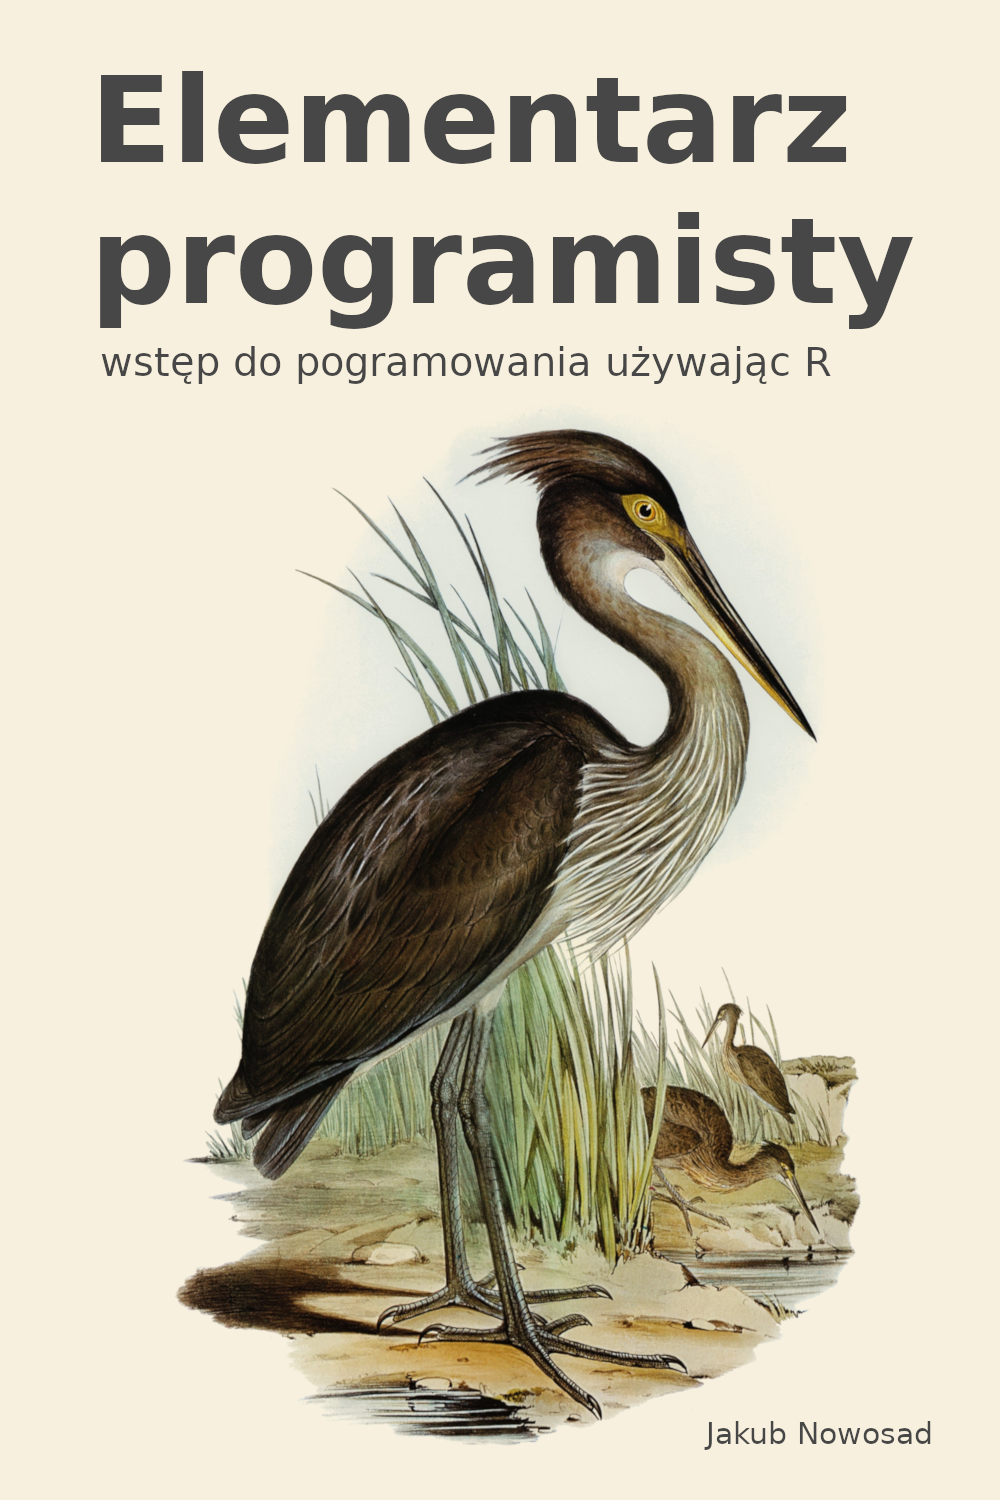
\includepdf{cover/cover_hr.png}

\let\maketitle\oldmaketitle
\maketitle

\thispagestyle{empty}
\vspace*{\fill}
Wydanie pierwsze, Poznań 2020 \\
Space A \\
Książka wydana na licencji Creative Commons BY \& SA \\
Więcej informacji \url{http://nowosad.github.io/elp/} \\
\\
\\
{\large ISBN: 978-83-953296-1-9}

{
\setcounter{tocdepth}{1}
\tableofcontents
}
\hypertarget{o-ksiux105ux17cce}{%
\chapter*{O książce}\label{o-ksiux105ux17cce}}
\addcontentsline{toc}{chapter}{O książce}

\textbf{Elementarz programisty: Wstęp do programowania używając R} ma na celu wprowadzenie do podstaw działania w języku R.
W pierwszej części, ``Podstawy'', opisuje ona w jaki sposób wykonywać proste operacje w R, czym są obiekty oraz jak tworzyć funkcje, które je przetwarzają.
Ta część zawiera także omówienie podstawowych narzędzi pozwalających na sterowanie przepływem informacji, takich jak wyrażenia warunkowe i pętle, metod działania na tekście, oraz sposobów wczytywania i zapisywania plików w różnych formatach.
Druga część, ``Narzędzia'', buduje na wiedzy zdobytej w części pierwszej i rozszerza ją.
Zawiera ona informacje na temat tworzenia funkcji przyjaznych użytkownikom oraz to w jaki sposób tworzyć odpowiednie komunikaty błędów, ostrzeżeń czy wiadomości.
W tej części następuje prezentacja metod analizy kodu, takich jak testy jednostkowe, benchmarking i profiling oraz sposobów rozwiązywania problemów z kodem używając technik debugowania.
Pokazanie są także możliwości łączenia R z innymi językami programowania C++ i Python.
Oprócz informacji ściśle powiązanych z R, \textbf{Elementarz programisty} ma także rozdział poświęcony systemom kontroli wersji - uniwersalnym narzędziom używanym przez programistów różnych języków.
Część ``Narzędzia'' kończy rozdział integrujący wiedzę z całej książki w postaci omówienia kolejnych kroków dotyczących tworzenia pakietów R.
\textbf{Elementarz programisty} zawiera też szereg praktycznych porad oraz wiele odnośników do dodatkowych materiałów, takich jak książki, blogi, kursy, czy strony internetowe.
Wszystkie rozdziały w tej książce dodatkowo zawierają zadania, które pozwalają na sprawdzenie i utrwalenie wiedzy.
Książka ta jest przeznaczona zarówno dla osób bez znajomości języków programowania, jak też dla osób, które znają inne języki programowania, ale są zainteresowane poznaniem języka R.
Uzyskana wiedza z tej książki daje podstawy do wykorzystywania R do różnorodnych celów, od analizy danych i opracowań statystycznych, poprzez tworzenie wykresów i wizualizacji, kończąc na aplikacjach specyficznych dla danej dziedziny.

Aktualna wersja książki znajduje się pod adresem \url{https://nowosad.github.io/elp/}.
Jeżeli używasz tej książki, zacytuj ją jako:

\begin{itemize}
\tightlist
\item
  Nowosad, J., (2020). Elementarz programisty: wstęp do programowania używając R. Poznań: Space A. Online: \url{https://nowosad.github.io/elp/}. ISBN: 978-83-953296-1-9
\end{itemize}

Zachęcam również do zgłaszania wszelkich uwag, błędów, pomysłów oraz komentarzy na stronie \url{https://github.com/nowosad/elp/issues}.

Ta książka jest dostępna na licencji Creative Commons Uznanie autorstwa - Użycie niekomercyjne - Bez utworów zależnych 4.0 Międzynarodowe.

\hypertarget{wymagania-wstux119pne}{%
\section*{Wymagania wstępne}\label{wymagania-wstux119pne}}
\addcontentsline{toc}{section}{Wymagania wstępne}

Do odtworzenia przykładów oraz do wykonania zadań zawartych w tej książce konieczne jest posiadanie aktualnej wersji \textbf{R}.
Pod adresem \url{https://cloud.r-project.org/} można znaleźć~instrukcje instalacji R dla systemów Windows, Mac OS i Linux.

W niektórych rozdziałach użyte zostanie zintegrowane środowisko programistyczne \textbf{RStudio}.
Można je zainstalować korzystając ze strony \url{https://www.rstudio.com/products/rstudio/download/\#download}.

Aspekty dotyczące kontroli wersji zostaną omówione używając oprogramowania \textbf{Git}.
Zalecanym sposobem instalacji Git na Windows jest wersja ze strony \url{https://gitforwindows.org/}.
Instrukcja instalacji na system Mac OS znajduje się~pod adresem \url{https://happygitwithr.com/install-git.html\#macos}.
Wersję Linuxową można zainstalować używając poniższej linii kodu:

\begin{verbatim}
# Ubuntu
sudo apt install git
\end{verbatim}

\begin{verbatim}
# Fedora
sudo dnf install git
\end{verbatim}

\hypertarget{styl-ksiux105ux17cki}{%
\section*{Styl książki}\label{styl-ksiux105ux17cki}}
\addcontentsline{toc}{section}{Styl książki}

W całej książce stosowana jest konwencja, w której \texttt{fun()} oznacza funkcje, \texttt{obi} oznacza nazwy obiektów, nazwy zmiennych oraz argumentów funkcji, a \texttt{sci/} oznacza ścieżki do plików.
Wszystkie pakiety użyte w tej książce oznaczane są pogrubioną czcionką - \textbf{pak}.

Tekst na szarym tle przedstawia blok kodu.
Może on zawierać komentarze (rozpoczynające się of znaku \texttt{\#}), kod oraz wynik jego użycia (rozpoczynające się od znaków \texttt{\#\textgreater{}}).

\begin{Shaded}
\begin{Highlighting}[]
\CommentTok{# komentarz}
\NormalTok{kod}
\CommentTok{#> wynik użycia kodu}
\end{Highlighting}
\end{Shaded}

Dodatkowo, ikona kompasu przedstawia dodatkowe informacje, alternatywne sposoby użycia funkcji, czy też~wskazówki.

\begin{rmdinfo}
Tutaj może znaleźć~się~dodatkowa informacja, alternatywny sposób użycia funkcji, czy też~wskazówka.
\end{rmdinfo}

\hypertarget{podziux119kowania}{%
\section*{Podziękowania}\label{podziux119kowania}}
\addcontentsline{toc}{section}{Podziękowania}

Książka została stworzona w R \citep{R-base} z wykorzystaniem pakietów \textbf{bookdown} \citep{R-bookdown}, \textbf{rmarkdown} \citep{R-rmarkdown}, \textbf{knitr} \citep{R-knitr} oraz programu \href{http://pandoc.org/}{Pandoc}.

Rysunek na okładce książki ``Great-billed Heron (Ardea rectirostris)'' został stworzony przez Elizabeth Gould do książki Birds of Australia Johna Goulda i został udostępniony na licencji CC0 1.0.

Ikony użyte w tej książce zostały stworzone przez Freepik z www.flaticon.com na licencji CC 3.0 BY.

\hypertarget{wprowadzenie}{%
\chapter{Wprowadzenie}\label{wprowadzenie}}

Żyjemy obecnie w epoce trzeciej rewolucji przemysłowej\footnote{Niektórzy wydzielają już nawet obecny czas jako czwartą rewolucję przemysłową - \url{https://en.wikipedia.org/wiki/Industry_4.0}.}, zwanej inaczej rewolucją cyfrową.
Jest ona powiązana z przejściem z technologii mechanicznych i analogowych na technologie elektroniczne i cyfrowe.
W tej epoce nastąpiło stworzenie i rozpowszechnieniem się komputerów, co w efekcie spowodowało szerokie zmiany społeczno-ekonomiczne.
Wiele z tych zmian jest pozytywnych, ale istnieją również zmiany negatywne, bądź też takie które trudno jednoznacznie ocenić.
Przykładowo, wyraźną korzyścią społeczną jest znacznie ułatwiony dostęp do informacji.
Jednocześnie taki dostęp powoduje sytuację~określaną jako przeciążenie informacją (ang. \emph{information overload}), w której występuje zbyt wielka ilość informacji aby podjąć właściwą decyzję lub zrozumieć sens danego tematu.

Rozwój technologiczny spowodował też transformację produkcji przemysłowej i zmiany gospodarcze.
Firmy zajmujące się~technologiami informacyjnymi, tj. Microsoft, Apple, czy Google, są obecnie jednymi z najbardziej dochodowych przedsiębiorstw, a twórca platformy Amazon, Jeff Bezos, jest najbogatszym człowiekiem świata\footnote{\url{https://en.wikipedia.org/wiki/The_World\%27s_Billionaires\#2018}}.
Wiele z tych technologii nie byłoby możliwych bez programowania.
Programowanie, w znacznym uproszczeniu, to proces tworzenia serii instrukcji, które informują komputer jak wykonać pewne zadanie.
Ta seria instrukcji jest zazwyczaj zapisywana na komputerze w postaci tekstu w wybranym języku programowania.
Co w takim razie powoduje, że programowanie ma tak istotny wpływ na wiele elementów codziennego życia?

Programowanie cechuje kilka unikatowych możliwości.
Po pierwsze, programowanie i jego efekty można w prosty sposób powielać niemal w nieskończoność.
Wcześniej stworzenie pewnego towaru opierało się o ograniczone zasoby, takie jak surowce naturalne.
Nie możliwe było wykucie zbroi raz, a następnie natychmiastowe powielenie jej wiele razy i sprzedanie jej wielu kopii.
We współczesnym świecie, jedna aplikacja może być sprzedana (lub rozpowszechniona) wiele razy, a często większy nacisk kładzie się na rozbudowę i ulepszanie istniejących popularnych aplikacji niż tworzenie nowych\footnote{Efektem tego jest też coraz większa popularność modeli subskrypcyjnych - \url{https://en.wikipedia.org/wiki/Subscription_business_model}.}.
Ułatwia to też budowę nowych rozwiązań na podstawie już istniejących\footnote{\url{https://en.wikipedia.org/wiki/Standing_on_the_shoulders_of_giants}}.
Współcześnie programowanie umożliwia wykonywanie trylionów (10\textsuperscript{18}) operacji arytmetycznych na sekundę\footnote{Przecięty człowiek jest w stanie wykonać około pół operacji na sekundę - \url{https://en.wikipedia.org/wiki/Computer_performance_by_orders_of_magnitude}.}.
Pozwala to na znaczne zwiększenie wydajności dostępnych rozwiązań (np. księgowość), otwiera możliwość praktycznego wykorzystania istniejących idei (np. modele klimatu), lub też~tworzenia nowych pomysłów (np. internet).
Inną cechą programowania jest też jego prosta możliwość automatyzacji powtarzanych czynności oraz ułatwiona powtarzalność (ang. \emph{reproducibility}).
Posiadając kod źródłowy danego oprogramowania lub skrypt wykonujący analizę danych, możliwe jest odtworzenie tego wyniku przez inną osobę na drugim końcu świata, lub też przez siebie samego po paru miesiącach.
Ostatnią cechą programowania jest jego uniwersalność.
Jest ono wykorzystywane w transporcie, przemyśle, nauce, rozrywce i wielu innych strefach życia.
W efekcie zrozumienie i znajomość języków programowania jest cenną~umiejętnością~we współczesnym świecie.

\hypertarget{mity-programistyczne}{%
\section{Mity programistyczne}\label{mity-programistyczne}}

Programowanie komputerowe ma obecnie już~długą historię - pierwszy język programowania Plankalkül powstał w latach 1943-1945\footnote{\url{https://en.wikipedia.org/wiki/Plankalk\%C3\%BCl}}.
Fortran, stworzony w roku 1957, jest nadal używany współcześnie do wielu celów, między innymi wymagających dużej wydajności obliczeń hydrologicznych, prognozowania pogody czy modelowania klimatu.
Programowanie ewoluowało i nadal ewoluuje wraz z rozwojem dostępności i możliwości komputerów, ale także wraz ze zmieniającymi się~potrzebami.
Pojawiły się nowe paradygmaty programowania oraz wiele nowych języków.
W tym samym czasie narosło również wiele mitów dotyczących programowania\footnote{Zobacz porównanie oczekiwań i rzeczywistej pracy programisty na \url{https://www.youtube.com/watch?v=HluANRwPyNo}.}.

Jednym z mitów jest to, że programowanie polega tylko siedzeniu przed ekranem komputera i wpisywaniu do niego kolejnych linii kodu.
Jest to oczywiście istotna część pracy programistycznej, ale prawdopodobnie nie jest ona nawet dominująca w przeciętym dniu programisty.
Wcześniej konieczne jest zastanowienie się jaki problem rozwiązujemy oraz zaprojektowanie możliwego rozwiązania tego problemu.
Stworzony kod może okazać się być nieprzystępny dla użytkownika, słabo zoptymalizowany, lub nawet błędny.
Dlatego też innym ważnym elementem jest testowanie kodu w celu wyłapania potencjalnych problemów.
Innym aspektem programowania jest tworzenie dokumentacji.
Żaden program nie może zachęcić do siebie użytkowników, jeżeli nie będą oni w stanie zrozumieć jak on działa.
Dokumentacja jest też cenna dla twórców programu, szczególnie kiedy konieczne jest użycie czy modyfikacja programu kilka miesięcy po jego ostatnim użyciu.
Programy komputerowe są też zazwyczaj w dużej sieci powiązań z już istniejącymi bibliotekami czy oprogramowaniem.
Zmiana w tych bibliotekach czy oprogramowaniu może skutkować nie zawsze oczekiwanymi zmianami w stworzonym programie.
Częścią programowania jest również~utrzymywanie istniejącego kodu źródłowego oraz jego ulepszanie.
Programiści do swojej pracy wykorzystują też~odpowiednie wspierające ich narzędzia, takie jak edytory kodu źródłowego, debugery, zintegrowane środowiska programistyczne czy systemy kontroli wersji.

Mitem również jest przekonanie, że programowanie to męskie zajęcie.
Bierze się ono z obecnej na rynku pracy struktury, w której około 75\% programistów to mężczyźni a tylko 25\% to kobiety.
Ta struktura jednak nie jest odzwierciedleniem jakichś~wrodzonych umiejętności.
Za pierwszego programistę często uważa się Adę Lovelace, angielskiego matematyka i poetkę\footnote{\url{https://en.wikipedia.org/wiki/Ada_Lovelace}}.
To ona w 1843 opublikowała pierwszy program komputerowy.
Jej algorytm do obliczenia liczb Bernoulliego nie został jednak przetestowany, ponieważ urządzenie do tych obliczeń (zwane maszyną analityczną\footnote{\url{https://en.wikipedia.org/wiki/Analytical_Engine}}) nie zostało skonstruowane.
Ponad wiek później, gdy istniały już techniczne możliwości tworzenia komputerów, programowanie było uważane za kobiecy zawód\footnote{\url{https://www.history.com/news/coding-used-to-be-a-womans-job-so-it-was-paid-less-and-undervalued}} (Rycina \ref{fig:marghamil}).
Z uwagi na szereg czynników społecznych i historycznych\footnote{\url{http://www.smbc-comics.com/?id=1883}}, w latach 1970 nastąpiło odwrócenie proporcji w tym zawodzie.
Obecnie podejmowanych jest szereg inicjatyw, które mają na celu zachęcić kobiety do programowania.
Wśród nich można wymienić działania organizacji \href{https://rladies.org/}{R-Ladies}, \href{https://www.pyladies.com/}{PyLadies}, \href{https://girlsjs.pl/}{girls.js}, czy \href{http://wimlds.org/}{Women in Machine Learning \& Data Science}.
Mit programisty mężczyzny jest też powiązany z wymienionym kilka akapitów niżej mitem samotnego programisty.



\begin{figure}[ht]

{\centering 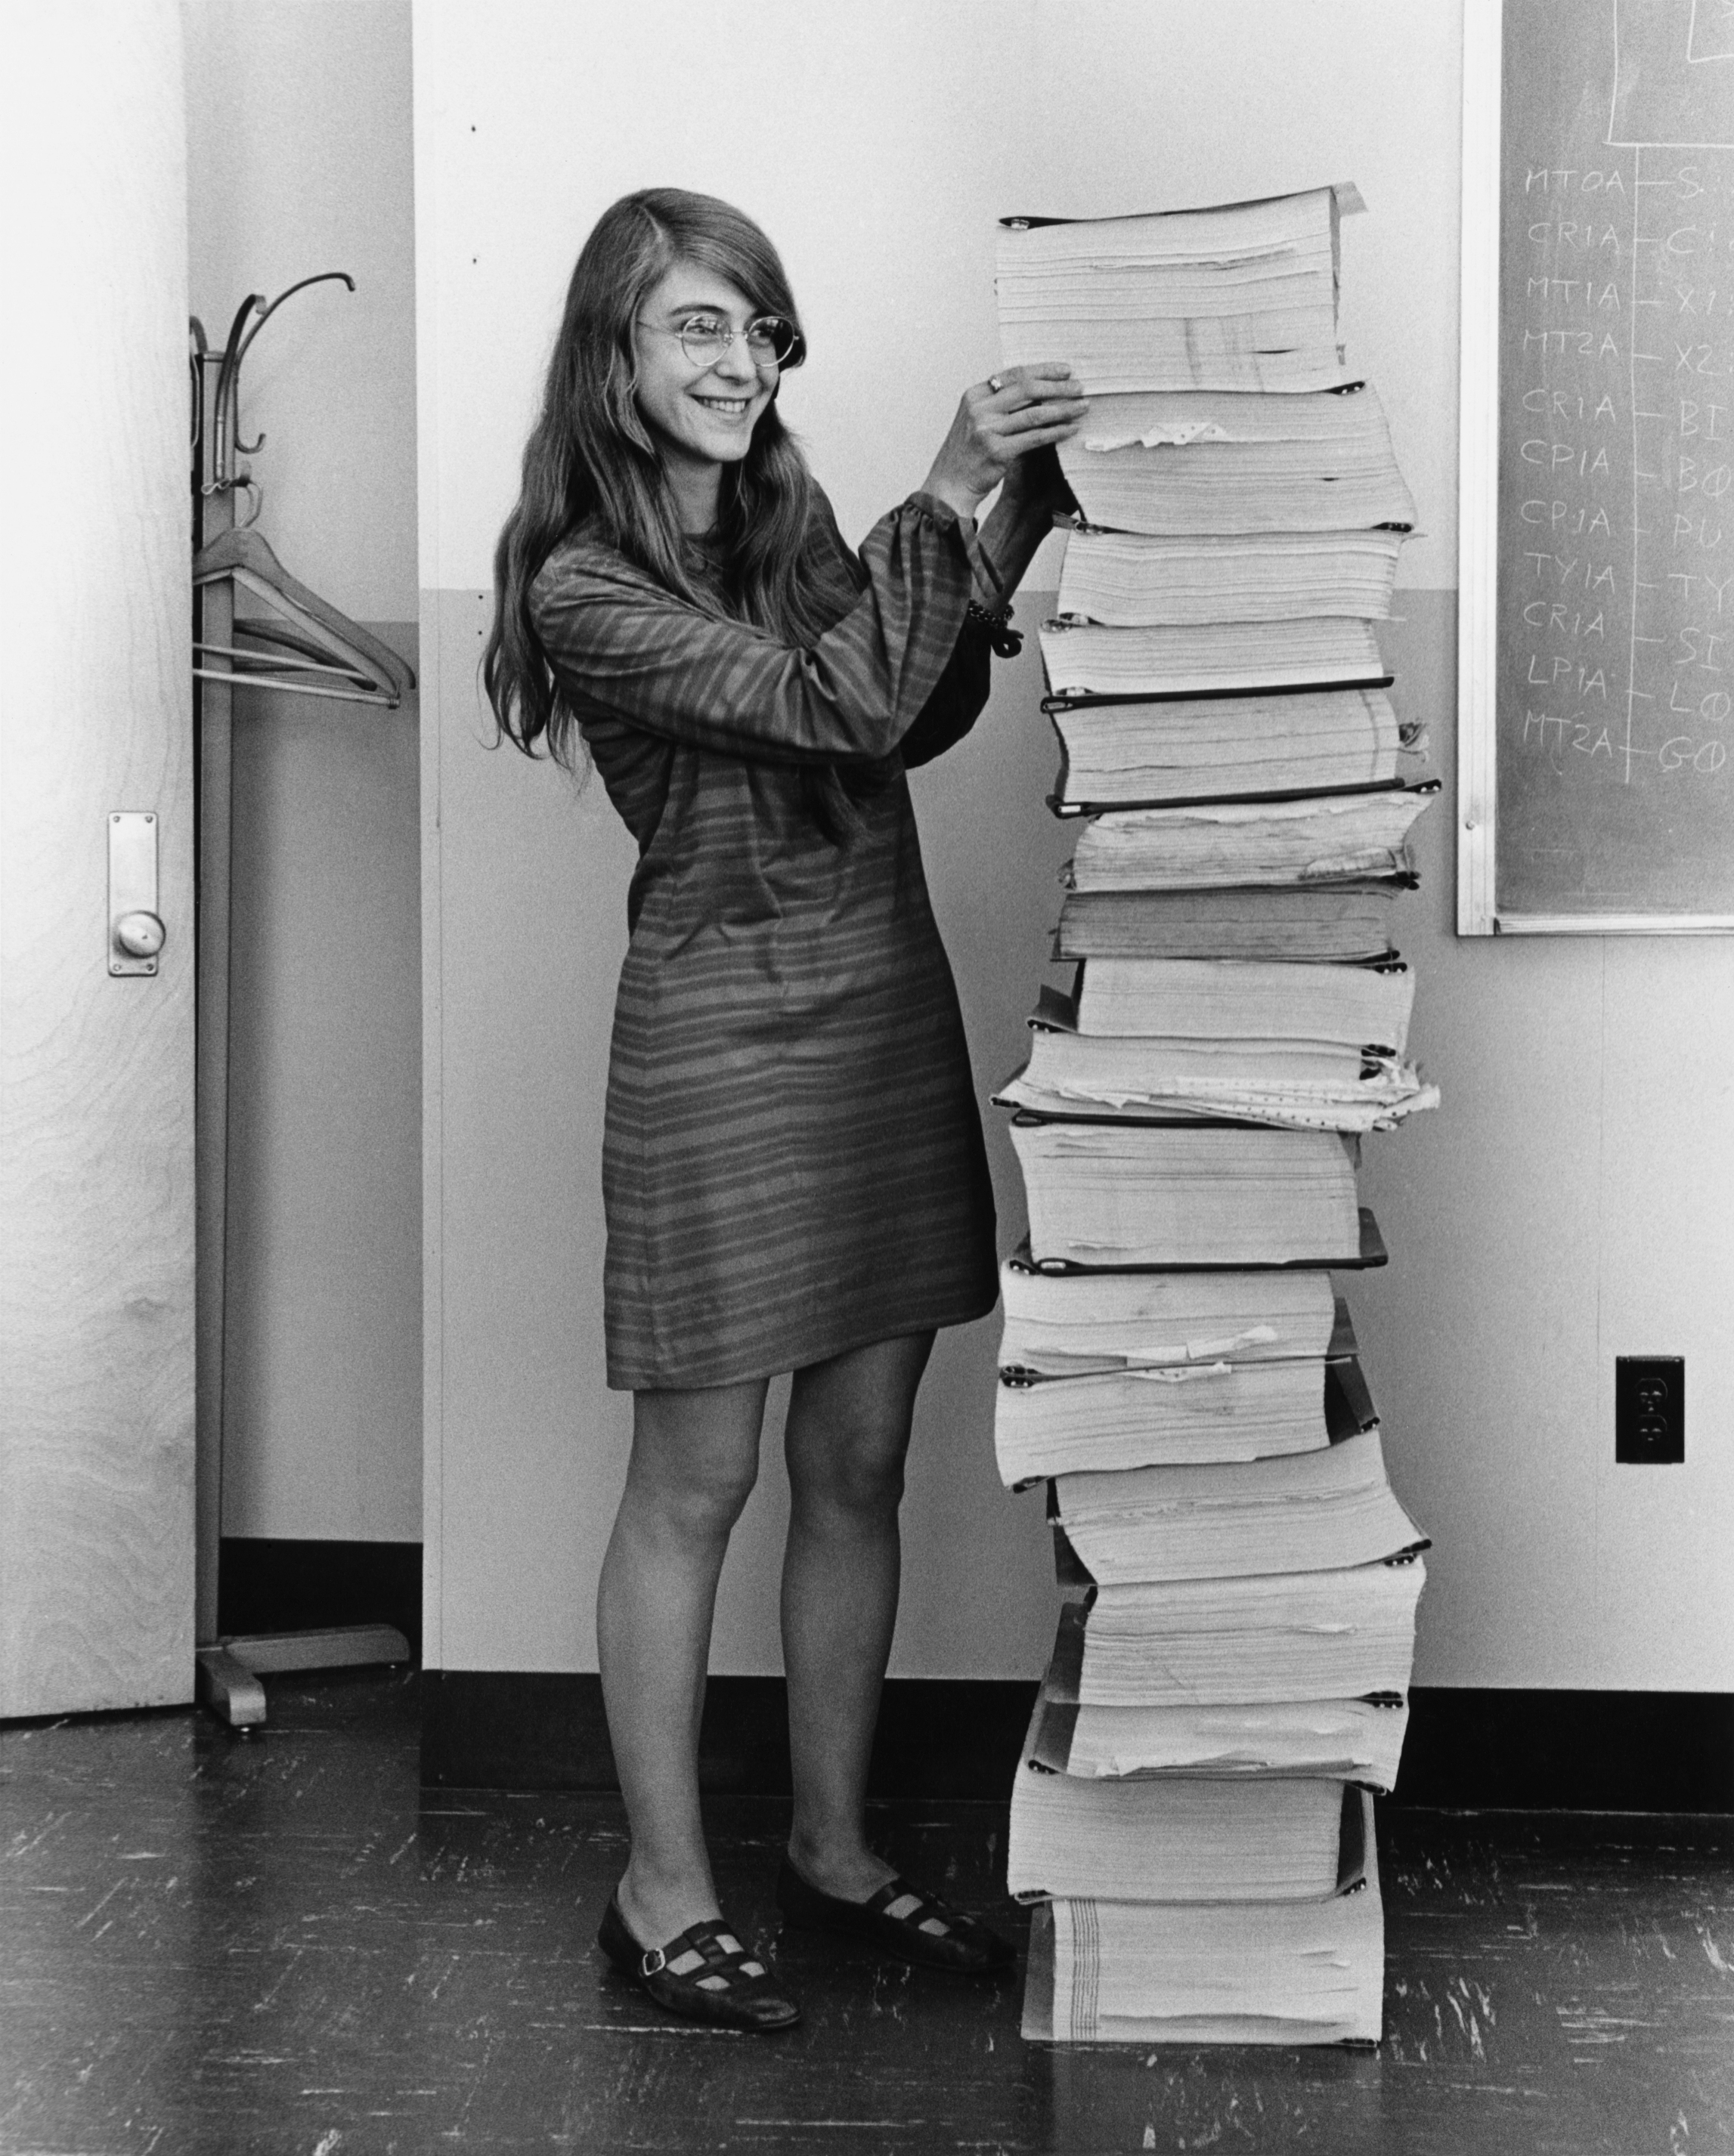
\includegraphics[width=0.8\linewidth]{images/margaret-hamilton} 

}

\caption{Margaret Hamilton stojąca w 1969 roku obok wydruków oprogramowania, które on i jej zespół stworzył na potrzeby misji Apollo. Źródło: \url{https://commons.wikimedia.org/wiki/File:Margaret_Hamilton_-_restoration.jpg}}\label{fig:marghamil}
\end{figure}

Kolejny jest mit wielkiego produktu.
Oznacza on, że po nauczeniu się~podstaw danego języka programowanie, jest się od razu w stanie stworzyć bardzo złożony program, np. nowy system operacyjny, skomplikowaną aplikację na telefon, czy grę komputerową.
W rzeczywistości takie produkty zazwyczaj opierają się o tysiące godzin pracy wielu programistów.
Dodatkowo, nie są one tworzone od podstaw, ale używając szeregu dostępnych narzędzi, bibliotek i innych rozwiązań.
Celem pisania kodu, więc nie powinno być stworzenie od zera bardzo złożonej aplikacji, lecz odpowiednie użycie istniejących rozwiązań.
Jednocześnie pisanie złożonego oprogramowania wymaga uzyskania niezbędnego doświadczenia.
Mit wielkiego produktu wiąże się również z wymienionym w kolejnym akapicie mitem samotnego programisty.

W popkulturze osoba, która potrafi programować spędza czas samotnie, gwałtownie wpisując kolejne linie kodu do komputera w ciemnym pokoju.
W rzeczywistości jednak większość profesjonalnych programistów pracuje w zespołach, których członkowie pracują nad różnymi aspektami tego samego problemu.
Pisanie programów często wymaga współpracy różnych osób, dlatego też umiejętność pracy w grupie jest coraz istotniejsza.
Warto dodać, że współpraca nad pisaniem programów nie musi odbywać się w jednym pokoju czy budynku.
Ze względu na charakter takiej pracy i możliwości technologiczne, wiele formalnych i nieformalnych grup pracuje zdalnie nad projektami.
Wiele przykładów takich zachowań można znaleźć przyglądając się~otwartemu oprogramowaniu (ang. \emph{open-source software}) na platformie GitHub (np. \url{https://github.com/trending/r}).

W poprzednim akapicie celowo użyłem stwierdzenia ``osoba, która potrafi programować'' zamiast ``programista''.
Jest to kolejny powszechny mit, że każda osoba która potrafi stworzyć program musi od razu zostać pełnoetatowym programistą.
Pisanie programów jest narzędziem, które ma wspomóc twórcę w pewnym celu.
Jednym z celów może być zostanie profesjonalnym deweloperem stron internetowych, aplikacji mobilnych, gier komputerowych, itd.
Nie jest to jednak jedyny cel - programowanie może być, na przykład przydatnym narzędziem w analizie danych\footnote{Wiąże się~to z popularnym na Zachodzie terminem \href{https://en.wikipedia.org/wiki/Data_science}{data science}, który łączy programowanie, analizę danych i wiedzę dziedzinową.}.
Umiejętności programistyczne są wykorzystywane przez ekonomistów, biologów, geografów i osób z wielu innych dziedzin.
Dodatkowo, podstawowe aspekty programowania są bardzo cenne w zawodach, w których ważna jest częsta współpraca z programistami.

Kolejny mitem jest mit programisty geniusza.
W tym micie programują tylko osoby, która ma nadludzką pamięć oraz wyróżniającą wiedzę matematyczną.
Oczywiście, takie cechy przydają się~w programowaniu, ale nie są do niego wymagane.
W programowaniu częściej od dobrej pamięci przydaje się umiejętność szybkiego znalezienia rozwiązania czy odpowiedzi na problem w internecie.
Programista nie musi znać na pamięć setek różnych poleceń i funkcji, ważne że umie je zidentyfikować.
Natomiast zamiast głębokiej wiedzy matematycznej do większości zadań programistycznych wystarczy podstawowa znajomość algebry.
Z tym mitem wiąże się~też inna kwestia - założenia że ten programista geniusz posiadł całą wiedzę programistyczną.
Podobnie jak nauka języka obcego, nauka języka programowania wymaga dużo pracy i czasu.
Dodatkowo, języki programowania czy techniki programowania zmieniają się~znacznie częściej niż języki naturalne, dlatego też częścią programowania jest ciągłe uczenie się.

Ostatni mit natomiast mówi o tym, że dla każdego problemu programistycznego istnieje tylko jedno najlepsze rozwiązanie.
Jeden problem można zazwyczaj rozwiązać na dziesiątki różnych sposobów.
Wynika to z tego, że wiele aspektów programowania opiera się~o personalne preferencje, np. wybór danego języka programowania, używanych bibliotek, czy stylu pisania kodu.
W efekcie zazwyczaj nie możliwe jest jednoznaczne określenie, które rozwiązanie jest lepsze, szczególnie jeżeli wiele rozwiązań ma podobną wydajność.
Istnieje jednak kilka reguł, z którymi zgadza się~większość programistów.
Pierwsza z nich mówi, że wolny działający kod jest lepszy niż szybki niedziałający kod\footnote{Parafrazując Donalda Kuntha ``We should forget about small efficiencies, say about 97\% of the time: premature optimization is the root of all evil. Yet we should not pass up our opportunities in that critical 3\%.''}.
Kolejna opiera się~o zasadę DRY (nie powtarzaj się, ang. \emph{Don't Repeat Yourself}), zalecającą unikanie różnego rodzaju powtórzeń wykonywanych przy programowaniu, np. używania tych samych fragmentów kodu w wielu miejscach.
Ostatnia reguła mówi, żeby tworzyć pisać programy w sposób modularny, czyli taki w którym każda funkcja spełnia tylko jedno i nie więcej zadanie, a złożone funkcje składają się z szeregu prostych funkcji.

\hypertarget{jezyki-programowania}{%
\section{Języki programowania}\label{jezyki-programowania}}

Głównym sposobem przekazywania instrukcji do komputera jest użycie języków programowania.
Pozwalają one na precyzyjny zapis zadań, które następnie mają zostać wykonane przez komputer.
Języki programowania składają się ze zbioru reguł syntaktycznych (składni) oraz semantyki.
Składnia (forma) mówi o tym jakie symbole są dostępne w danym języku oraz jak te symbole mogą być łączone w większe struktury.
Semantyka (treść) natomiast definiuje znaczenie poszczególnych symboli.

W przeciwieństwie do języków naturalnych, języki programowania wymagają wysokiej precyzji.
Mówiąc w języku naturalnym możemy popełnić jakiś błąd (np. gramatyczny czy składniowy) i nadal być łatwo zrozumianym przez otoczenie.
Języki programowania nie akceptują takich błędów i nie są w stanie wykonać danego polecenia.
Obecnie istnieją tysiące\footnote{\url{http://codelani.com/lists/languages.html}} języków programowania i każdego roku powstają nowe.
Nie ma wśród nich jednego najlepszego, uniwersalnego języka programowania i w najbliższej przyszłości ten stan się~nie zmieni.
Jest to związane z bardzo szerokim zastosowaniem programowania w wielu dziedzinach czy problemach, które mają od siebie zupełnie różne wymagania.
Przykładowe wymagania mogą~dotyczyć np. szybkości wykonywanych obliczeń, łatwości pisania kodu, stabilności języka programowania, czy celu obliczeń.
Do tego dochodzą również rożne kwestie historyczne i społeczne, jak na przykład preferowanie danego języka programowania przez osoby w danej branży.
Obecnie wśród najpopularniejszych języków programowania można wymienić takie języki jak Java, C, Python, C++, Visual Basic .NET, JavaScript, C\#, PHP, SQL, Objective-C, język asemblera, Perl, czy R.
Języki programowania można podzielić na wiele różnych grup w zależności od przyjętych kryteriów.
Poniżej wyjaśnionych jest kilka możliwych podziałów języków programowania.

Jednym z nich jest sposób wykonywania kodu - to czy kod w danym języku jest kompilowany czy też interpretowany.
Kompilacja kodu (np. C czy Java) polega na jego tłumaczeniu do postaci języka maszynowego.
W efekcie zapewnia to wysoką wydajność programu, ale za to kod jest ściśle powiązany z daną platformą sprzętową.
Programowanie w językach kompilowanych jest zazwyczaj bardziej złożone i trudniejsze w nich jest odnajdywanie błędów (tzw. debugging).
Interpretowane języki programowania (np. R czy Python), często również nazywane językami skryptowymi, charakteryzuje to,
że w momencie uruchomienia kod jest zamieniany na postać zrozumiałą dla komputera i od razu wykonywany.
W efekcie można szybko zobaczyć efekt zmian.
Wadą tego typu języków jest ich zmniejszona wydajność w porównany do języków kompilowanych.

Innym powszechnym podziałem języków programowania jest ich rozróżnianie na podstawie poziomu.
Tutaj można wyróżnić języki od niskiego poziomu do wysokiego poziomu.
Na najniższym poziomie jest język maszynowy, czyli taki w którym zapis programu wyrażony jest w postaci liczb binarnych.
Powyżej są umieszczony jest język asemblera, w którym program jest zapisany poprzez serię instrukcji.
Na najwyższym poziomie stawia się języki, które są wspomagane przez kompilator albo interpreter.

Języki programowania można też rozróżnić ze względu na paradygmat programowania.
Definiuje on w jaki sposób w danym języku wykonywany jest przepływ sterowania czy też jak kod jest organizowany.
Dwa podstawowe paradygmaty programowania to programowanie imperatywne i deklaratywne.
Programowanie imperatywne (np. Fortran, C) opisuje proces wykonywania kodu jako sekwencję instrukcji zmieniających stan programu.
Obejmuje ono inne paradygmaty, jak na przykład programowanie proceduralne czy obiektowe.
Programowanie deklaratywne skupia się natomiast na warunkach jakie musi spełniać końcowe rozwiązanie, a nie na sekwencji kroków do jego stworzenia.
W skład tej grupy wchodzi, między innymi, programowanie funkcyjne czy matematyczne.
Niektóre języki mogą być zaklasyfikowane do kilku paradygmatów.
Przykładowo R wspiera zarówno paradygmat funkcyjny, ale zawiera też możliwości programowania obiektowego.

\hypertarget{r}{%
\section{R}\label{r}}

W tej książce wprowadzenie do programowania opiera się o język \href{https://www.r-project.org/}{R} (Rycina \ref{fig:rlogo}).

\begin{figure}[H]

{\centering 
\includegraphics[width=0.25\linewidth]{images/Rlogo} 

}

\caption{Logo języka programowania R.}\label{fig:rlogo}
\end{figure}

Wynika to z szeregu zalet tego języka:

\begin{itemize}
\tightlist
\item
  R jest bezpłatnym, otwartym oprogramowaniem, który można uruchomić na różnych systemach operacyjnych (Windows, Mac OS i Linux), zarówno na komputerach osobistych jak i na dużych klastrach obliczeniowych.
  W efekcie nie ma on finansowej bariery rozpoczęcia pracy, a kod napisany na jednym komputerze można również przenieść i uruchomić na innym sprzęcie.
\item
  R jest językiem interpretowalnym, czyli wykonanie w nim komend nie wymaga kompilacji.
  Ten aspekt ułatwia szybsze zrozumienie działania tego języka.
\item
  R posiada wiele wbudowanych narzędzi analizy i wizualizacji danych.
  Pozwala to na relatywnie szybkie osiąganie wymiernych efektów z korzystania z tego języka.
\item
  R posiada tysiące dodatkowych rozszerzeń (zwanych pakietami) pozwalających na, między innymi, przetwarzanie różnorodnych danych, ich wizualizację, czy zaawansowane modelowanie.
  Oficjalnym portalem zawierającym dodatkowe pakiety R jest \href{https://cran.r-project.org/}{CRAN}.
\item
  R ma przyjazną społeczność użytkowników tego języka, zarówno online jak i spotykających się na żywo na tzw. meetupach.
\item
  W celu ułatwienia pracy z R powstało również zintegrowane środowisko programistyczne RStudio, które wspomaga pisanie i analizę kodu w R.
\item
  R został zaprojektowany jako narzędzie ułatwiające komunikację między różnymi językami programowania, głównie C oraz Fortran\footnote{\url{https://www.youtube.com/watch?v=_hcpuRB5nGs}}.
  Obecnie R pozwala na łatwe łączenie kodu pochodzącego również z takich języków jak C++, Python, JavaScript, itd.
\item
  R jest używany przez wiele małych firm, jak i wielkich korporacji, wliczając w to BBC, Facebook, Google, Microsoft, Mozilla, Netflix, T-Mobile, czy Uber\footnote{\url{https://github.com/ThinkR-open/companies-using-r}}.
\end{itemize}

Oczywiście, uniwersalny i idealny język nie istnieje:

\begin{itemize}
\tightlist
\item
  R jest językiem interpretowalnym, czyli wykonanie w nim komend nie wymaga kompilacji.
  W efekcie R nie jest najszybszym językiem programowania.
\item
  Podobnie jak wiele innych języków, również R zawiera wiele niekonsekwencji, wynikających z wieloletniej ewolucji tego języka.
  W efekcie istnieje wiele specjalnych przypadków czy wyjątków, które warto znać \citep{burns2012r}.
\end{itemize}

Ta książka skupia się~na prezentacji głównym konceptów programistycznych używając języka R.
W sekcji \ref{resources} można znaleźć listę różnorodnych materiałów, książek, blogów, kursów, czy serwisów ułatwiających i wspomagających naukę R.
Istnieje także wiele wprowadzających materiałów do nauki innych języków.
Przykładowo, osoby zainteresowane nauką Pythona mogą skorzystać z istniejących książek (\citet{gries2017practical} oraz \citet{guzdial2016introduction}), czy też kursów \href{http://swcarpentry.github.io/python-novice-inflammation/}{Software Carpentry} oraz \href{https://www.python-course.eu/python3_course.php}{Python Course}.
W pracy programistycznej przydaje się również często znajomość linii komend.
Tutaj również można użyć materiałów z kursu \href{https://swcarpentry.github.io/shell-novice/}{Software Carpentry} lub książki \href{https://seankross.com/the-unix-workbench/}{The Unix Workbench} \citep{krossUnixWorkbench2017}.

\hypertarget{zadania}{%
\section{Zadania}\label{zadania}}

\begin{enumerate}
\def\labelenumi{\arabic{enumi})}
\tightlist
\item
  Pomyśl do czego jesteś w stanie wykorzystać programowanie w swoim życiu zawodowym lub prywatnym?
\item
  Zastanów się nad mitami związanymi z programowaniem.
  Czy jesteś w stanie wskazać jakieś mity nie wymienione powyżej?
\item
  Wybierz trzy języki programowania z listy wymienionej w tym rozdziale i poszukaj informacji o nich.
  Do czego są one stosowane?
  Jakie mają wady i zalety?
\end{enumerate}

\hypertarget{part-podstawy}{%
\part{Podstawy}\label{part-podstawy}}

\hypertarget{ergosum}{%
\chapter{Start R}\label{ergosum}}

Wykonywanie kodu w języku interpretowalnym, jakim jest R, może odbywać się~poprzez wpisanie polecenia w oknie konsoli (zwanej też terminalem) i jego uruchomienie\footnote{To jest tzw. tryb interaktywny.
  Istnieje również tryb skryptowy, o którym więcej informacji można znaleźć w kolejnym rozdziale.}.
Komendy są najpierw sprawdzanie pod kontekstem ich poprawności.
Polega to na określeniu, np. czy podana funkcja lub inny obiekt istnieje, czy nie zostały użyte niedozwolone znaki, lub czy wszystkie nawiasy czy cudzysłowy zostały zamknięte.
Języki programowania są w tym aspekcie bardziej bezwzględne niż języki naturalne - nie potrafią one zrozumieć wyrażeń zawierających nawet niewielkie błędy takie jak, np. użycie dużej litery zamiast małej.

\hypertarget{wyraux17cenia}{%
\section{Wyrażenia}\label{wyraux17cenia}}

Podstawowe działania arytmetyczne, dodawanie, odejmowane, mnożenie i dzielenie, są również często używane w wielu językach programowania.
Dla każdej z tych operacji istnieje odpowiedni operator w R.
Operatorem dodawania jest \texttt{+}.

\begin{Shaded}
\begin{Highlighting}[]
\DecValTok{2} \OperatorTok{+}\StringTok{ }\DecValTok{2}
\CommentTok{#> [1] 4}
\end{Highlighting}
\end{Shaded}

Operatorem odejmowania jest \texttt{-}.

\begin{Shaded}
\begin{Highlighting}[]
\DecValTok{1} \OperatorTok{-}\StringTok{ }\DecValTok{3}
\CommentTok{#> [1] -2}
\end{Highlighting}
\end{Shaded}

Operatorem mnożenia jest \texttt{*}.

\begin{Shaded}
\begin{Highlighting}[]
\DecValTok{5} \OperatorTok{*}\StringTok{ }\DecValTok{5}
\CommentTok{#> [1] 25}
\end{Highlighting}
\end{Shaded}

Operatorem dzielenia jest \texttt{/}.

\begin{Shaded}
\begin{Highlighting}[]
\DecValTok{42} \OperatorTok{/}\StringTok{ }\DecValTok{5}
\CommentTok{#> [1] 8.4}
\end{Highlighting}
\end{Shaded}

Wszystkie powyższe operacje można wykonać poprzez ich wpisanie w oknie konsoli R i naciśnięcie klawisza Enter.

\hypertarget{obiekty}{%
\section{Obiekty}\label{obiekty}}

\begin{quote}
``Dwa slogany są pomocne w zrozumieniu obliczeń w R: 1. Wszystko co istnieje jest obiektem. 2. Wszystko co się dzieje jest wywołaniem funkcji.'' John Chambers
\end{quote}

Powyższy cytat sugeruje dwa najważniejsze elementy języka R: obiekty i funkcje.
Zrozumienie w jaki sposób się je tworzy i zmienia będzie w związku z tym, konieczną wiedzą osób piszących w tym języku.

\hypertarget{operator-przypisania}{%
\subsection{Operator przypisania}\label{operator-przypisania}}

Nadanie wartości do obiektu wykonuje się używając operatora przypisania\footnote{Jest to pewne uproszczenie - \url{https://adv-r.hadley.nz/names-values.html\#binding-basics}.}.
R posiada trzy operatory przypisania, które mają niemal identyczne działanie\footnote{Więcej informacji na temat różnic w działaniu tych operatorów można znaleźć na stronie \url{https://stackoverflow.com/questions/1741820/what-are-the-differences-between-and-in-r}.}: \texttt{=}, \texttt{\textless{}-}, \texttt{-\textgreater{}}.
Warto wybrać jeden z tych operatorów i konsekwentnie używać go pisząc kod.
W tej książce jako główny operator przypisania będzie używany znak \texttt{=}.

W poniższej linii stworzony jest nowy obiekt, o nazwie \texttt{x}, który zawiera wartość \texttt{7}.

\begin{Shaded}
\begin{Highlighting}[]
\NormalTok{x =}\StringTok{ }\DecValTok{7}
\end{Highlighting}
\end{Shaded}

Można to sprawdzić wpisując nazwę tego obiektu.

\begin{Shaded}
\begin{Highlighting}[]
\NormalTok{x}
\CommentTok{#> [1] 7}
\end{Highlighting}
\end{Shaded}

Operatory przypisania może również posłużyć do nadania wartości z jednego obiektu do drugiego.
Poniżej nowy obiekt \texttt{y} przyjmuje wartość od obiektu \texttt{x}.

\begin{Shaded}
\begin{Highlighting}[]
\NormalTok{y =}\StringTok{ }\NormalTok{x}
\NormalTok{y}
\CommentTok{#> [1] 7}
\end{Highlighting}
\end{Shaded}

Język R przechowuje i przetwarza wszystkie obiekty w pamięci komputera (RAM).
Wpływa to na zwiększoną wydajność i elastyczność obliczeń, ale jednocześnie powoduje to ograniczenie wielkości obiektów na jakich można pracować.
Istnieje równocześnie \href{https://bookdown.org/rdpeng/RProgDA/working-with-large-datasets.html}{szereg strategii} jak postępować z większymi zbiorami danych, które nie mieszczą się~w RAMie \citep{pengMasteringSoftwareDevelopment2017}.

\hypertarget{dzialania-na-obiektach}{%
\subsection{Działania na obiektach}\label{dzialania-na-obiektach}}

Każdy stworzony obiekt w R może być następnie używany do kolejnych operacji, a w efekcie też tworzenia nowych obiektów.
W poniższych czterech przypadkach obiekt \texttt{x} został przetworzony używając operatorów dodawania, odejmowania, mnożenia oraz dzielenia, a jako wyniki tych obliczeń powstały nowe obiekty.

\begin{Shaded}
\begin{Highlighting}[]
\NormalTok{z1 =}\StringTok{ }\NormalTok{x }\OperatorTok{+}\StringTok{ }\DecValTok{3}
\NormalTok{z1}
\CommentTok{#> [1] 10}
\NormalTok{z2 =}\StringTok{ }\NormalTok{x }\OperatorTok{-}\StringTok{ }\DecValTok{5}
\NormalTok{z2}
\CommentTok{#> [1] 2}
\NormalTok{z3 =}\StringTok{ }\NormalTok{x }\OperatorTok{*}\StringTok{ }\DecValTok{2}
\NormalTok{z3}
\CommentTok{#> [1] 14}
\NormalTok{z4 =}\StringTok{ }\NormalTok{x }\OperatorTok{/}\StringTok{ }\DecValTok{4}
\NormalTok{z4}
\CommentTok{#> [1] 1.75}
\end{Highlighting}
\end{Shaded}

\begin{rmdinfo}
Część języków programowania, np. C, wymaga zadeklarowania zmiennej przed jej użyciem poprzez podanie jej typu i nazwy.
Wybór typu zmiennej w tych językach może mieć widoczne konsekwencje.
Przykładowo, jeżeli obiekt \texttt{x} zostanie zadeklarowany jako liczba całkowita (integer), wynikiem dzielenia \texttt{x\ /\ 4} będzie \texttt{1} zamiast \texttt{1.75}.
\end{rmdinfo}

Działania na obiektach mogą też się odbywać używając innych operatorów oraz różnorodnych funkcji.
Przykładowo, operator zapisywany jako \texttt{\%\%} to modulo, którego celem jest określanie reszty z dzielenia.

\begin{Shaded}
\begin{Highlighting}[]
\NormalTok{z5 =}\StringTok{ }\NormalTok{x }\OperatorTok\StringTok{ }\DecValTok{3}
\NormalTok{z5}
\CommentTok{#> [1] 1}
\end{Highlighting}
\end{Shaded}

Operator \texttt{\%/\%} przedstawia dzielenie całkowite.

\begin{Shaded}
\begin{Highlighting}[]
\NormalTok{z6 =}\StringTok{ }\NormalTok{x }\OperatorTok\StringTok{ }\DecValTok{3}
\NormalTok{z6}
\CommentTok{#> [1] 2}
\end{Highlighting}
\end{Shaded}

Operator \texttt{\^{}} natomiast wykonuje podniesienie wartości obiektu do wybranej potęgi.

\begin{Shaded}
\begin{Highlighting}[]
\NormalTok{z7 =}\StringTok{ }\NormalTok{x}\OperatorTok{^}\DecValTok{2}
\NormalTok{z7}
\CommentTok{#> [1] 49}
\end{Highlighting}
\end{Shaded}

Odwrotnością potęgowania jest pierwiastkowanie.
W R nie istnieje do tego celu specjalny operator, ale zawiera on funkcję \texttt{sqrt()}.

\begin{Shaded}
\begin{Highlighting}[]
\NormalTok{z8 =}\StringTok{ }\KeywordTok{sqrt}\NormalTok{(x)}
\NormalTok{z8}
\CommentTok{#> [1] 2.65}
\end{Highlighting}
\end{Shaded}

Często używaną funkcją w R jest też \texttt{c()}.
Ta funkcja łączy krótsze wektory w dłuższe wektory.

\begin{Shaded}
\begin{Highlighting}[]
\NormalTok{z9 =}\StringTok{ }\KeywordTok{c}\NormalTok{(z2, z4, z8)}
\NormalTok{z9}
\CommentTok{#> [1] 2.00 1.75 2.65}
\end{Highlighting}
\end{Shaded}

\begin{rmdinfo}
Operatory użyte w tym rozdziale, np. \texttt{+}, \texttt{*}, \texttt{\^{}}, \texttt{\%\%} to też są funkcje, ale zapisane w skrótowej formie ułatwiającej z nimi pracę.
Te operatory można też użyć jako normalne funkcje poprzez dodanie znaku zwanego grawisem - ``\texttt{\textasciigrave{}}'', np. \texttt{2\ +\ 2} można też~zapisać jako \texttt{\textasciigrave{}+\textasciigrave{}(2,\ 2)}.
\end{rmdinfo}

\hypertarget{ide}{%
\section{IDE}\label{ide}}

Zintegrowane środowisko programistyczne (ang. \emph{Integrated Development Environment}, IDE) to program ułatwiający pisanie kodu.
Zawiera on wiele użytecznych funkcjonalności, takich jak wbudowany edytor i konsola, podświetlanie składni, automatyczne uzupełnianie kodu, itd.
Bez IDE kod musi być pisany w jednym programie, a następnie kopiowany i uruchamiany w innym.

Do popularnych IDE dla R należą:

\begin{itemize}
\tightlist
\item
  RStudio
\item
  Emacs + ESS
\item
  vim + Nvim-R
\item
  Visual Studio + RTVS
\end{itemize}

W tej książce będzimy korzystać z pierwszego z nich.
RStudio to zintegrowane środowisko programistyczne pierwotnie stworzone dla R.

\begin{rmdinfo}
RStudio to nie jest to samo co R.
R jest językiem programowania, podczas gdy RStudio to aplikacja ułatwiająca pisanie kodu.
Możliwe jest używanie R bez RStudio, ale RStudio bez R nie pełni już~swojej roli.
Częstą analogią~jest porównanie samochodowe, w którym R jest opisywany jako silnik a RStudio jako deska rozdzielcza.
\end{rmdinfo}

\begin{figure}[H]

{\centering 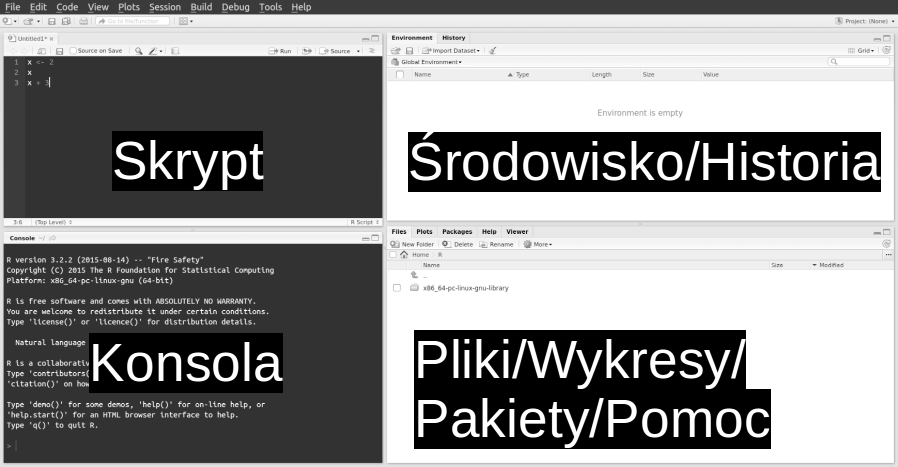
\includegraphics[width=\textwidth]{images/rstudio-ide} 

}

\caption{Okno RStudio z opisaną funkcjonalnością każdej z jego części.}\label{fig:rstudioimage}
\end{figure}

Typowa praca w RStudio często polega na wpisywaniu poleceń do pliku tekstowego widocznego w części skryptowej (rycina \ref{fig:rstudioimage}), a następnie wykonywaniu kolejnych linii kodu w oknie konsoli używając skrótu klawiaturowego CTRL+ENTER (więcej przydatnych skrótów klawiaturowych można znaleźć w tabeli \ref{tab:rstudiosk}).
Efektem wykonywania funkcji może być powstanie nowych obiektów, które można zobaczyć w oknie ``środowiska'' lub też wyświetlenie grafik, które można zobaczyć w oknie ``wykresu'' (rycina \ref{fig:rstudioimage}).

Dobrą praktyką pracy z R w RStudio jest też używanie projektów RStudio (ang. \emph{RStudio projects}).
Projekt jest to folder zawierający wszystkie skrypty i pozostałe pliki powiązane z jakimś zadaniem (np. analizą danych, czy stworzeniem nowego pakietu R).
Ułatwia on przenoszenie kodu pomiędzy różnymi komputerami, a także daje dostęp do szeregu dodatkowych możliwości w RStudio.

Aby stworzyć pierwszy projekt RStudio, należy:

\begin{enumerate}
\def\labelenumi{\arabic{enumi}.}
\tightlist
\item
  Kliknąć \texttt{File\ -\textgreater{}\ New\ Project}.
\item
  Wybrać \texttt{New\ Directory}.
\item
  Wybrać \texttt{New\ Project}.
\item
  Podać nazwę nowego projektu, np. ``programowanie1'' oraz wybrać miejsce na dysku, gdzie ma się~nowy projekt znajdować.
\item
  Jeżeli możliwe, to wybrać też~opcję \texttt{Create\ a\ git\ repository}.
\item
  Kliknąć \texttt{Create\ Project}.
\end{enumerate}

W ten sposób zostanie utworzony nowy folder wraz z plikiem o nazwie projektu z rozszerzeniem \texttt{.Rproj}, np. \texttt{programowanie1.Rproj}.
Ten folder staje się też od razu folderem roboczym (więcej na ten temat znajdziesz w rozdziale \ref{io}).
Otwarcie wcześniej stworzonego projektu ma miejsce poprzez uruchomienie pliku z rozszerzeniem \texttt{.Rproj} lub też wybór projektu w prawym górnym rogu RStudio.

\begin{table}

\caption{\label{tab:rstudiosk}Podstawowe skróty klawiaturowe w RStudio}
\centering
\begin{tabular}[t]{>{\raggedright\arraybackslash}p{12em}>{\raggedright\arraybackslash}p{18em}}
\toprule
Skrót & Wyjaśnienie\\
\midrule
Ctrl+Enter & Wykonuje wybraną linię kodu w skrypcie R\\
Tab & Uzupełnia kod (podaje pasujące możliwości)\\
F1 & Wyświetla plik pomocy dla wybranej funkcji\\
Ctrl+Shift+C & Ustawia wybrane linie jako komentarz/odkomentuj fragment kodu\\
strzałka Góra/Dół (w oknie konsoli) & Wybiera wcześniej wpisany kod\\
\addlinespace
Esc & Przerywa niedokończoną operację\\
Shift+Alt+K & Wyświetla listę skrótów klawiaturowych\\
\bottomrule
\end{tabular}
\end{table}

\hypertarget{styl}{%
\section{Styl}\label{styl}}

Języki programowania pozwalają na napisanie dokładnie tego samego kodu na wiele sposobów.
Przykładowo \texttt{z1\ =\ x\ +\ 3} ma identyczne działanie jak \texttt{z1=x+3}.
Styl pisania kodu obejmuje, między innymi, sposoby nazywania obiektów, stosowania odstępów czy wcięć, czy też pisania komentarzy.
Przyjęcie wybranego stylu pozwala na ułatwienie czytania i zrozumienia kodu oraz zmniejszenie szans na powstawanie w nim błędów.

Poniżej znajdują się podstawowe porady dotyczące stylu pisania kodu.
Więcej wskazówek można znaleźć na w \href{https://style.tidyverse.org/}{poradniku stylu RStudio} oraz \href{https://google.github.io/styleguide/Rguide.xml}{poradniku stylu Google}.
Oba te poradniki nie są identyczne i czasami zawierają sprzeczne porady.
Najważniejsze jest, aby wybrać jeden odpowiadający piszącemu kod styl i się~go konsekwentnie trzymać.

\hypertarget{nazwy-obiektow}{%
\subsection{Nazwy obiektów}\label{nazwy-obiektow}}

Istnieje wiele konwencji nazywania obiektów\footnote{\url{https://en.wikipedia.org/wiki/Naming_convention_(programming)}}.
Najczęściej używaną konwencją w R jest tzw. \href{https://en.wikipedia.org/wiki/Snake_case}{``snake case''}.
Polega ona na tworzeniu nazw obiektów składających się ze słów połączonych znakiem podkreślenia (\texttt{\_}).
Ważne, żeby nazwy obiektów ułatwiały zrozumienie ich zawartości.

\begin{Shaded}
\begin{Highlighting}[]
\CommentTok{# obiekt}
\NormalTok{bok_a}
\NormalTok{bok_b}

\CommentTok{# funkcja}
\NormalTok{pole_prostokata}
\end{Highlighting}
\end{Shaded}

Nazwa obiektu nie może zaczynać się od liczby, ani nie może używać specjalnych symboli, tj. \texttt{\^{}}, \texttt{!}, \texttt{\$}, \texttt{@}, \texttt{+}, \texttt{-}, \texttt{/}, czy \texttt{*}.
Dodatkowo należy uważać, żeby nowa nazwa obiektu nie nadpisała istniejącego obiektu lub funkcji.
Nie powinno nazywać się obiektów tak jak istniejące funkcje, np. \texttt{c}, \texttt{t}, \texttt{table}, itd.

\hypertarget{odstux119py}{%
\subsection{Odstępy}\label{odstux119py}}

Odstępy pełnią bardzo ważną funkcję przy pisaniu kodu, podobnie jak odstępy przy pisaniu tekstu.
Wyobraź sobie czytanie powieści, w której nie ma żadnych odstępów między słowami czy rozdziałami.
Często mówi się, że ``kod musi oddychać'' - odstępy zwiększają czytelność kodu i pozwalają na jego szybsze zrozumienie oraz ułatwiają naprawienie występujących błędów.

Odstępy można uzyskać poprzez użycie spacji.
Spacje powinny być użyte po przecinkach, ale nigdy przed nimi.
Dodatkowo, większość operatorów (np. \texttt{=}, \texttt{+}, \texttt{-}, \texttt{==}) powinna być otoczona przez spacje.

\begin{Shaded}
\begin{Highlighting}[]
\CommentTok{# Zalecane}
\NormalTok{srednia =}\StringTok{ }\KeywordTok{mean}\NormalTok{(wartosc, }\DataTypeTok{na.rm =} \OtherTok{TRUE}\NormalTok{)}
\NormalTok{pole =}\StringTok{ }\NormalTok{bok_a }\OperatorTok{*}\StringTok{ }\NormalTok{bok_b}

\CommentTok{# Niewskazane}
\NormalTok{srednia=}\KeywordTok{mean}\NormalTok{ ( wartosc,}\DataTypeTok{na.rm=}\OtherTok{TRUE}\NormalTok{ ) }
\NormalTok{pole=bok_a}\OperatorTok{*}\NormalTok{bok_b}
\end{Highlighting}
\end{Shaded}

Spacje należy również używać do tworzenia wcięć - każde z nich powinno się składać z dwóch spacji.

\begin{Shaded}
\begin{Highlighting}[]
\CommentTok{# Zalecane}
\NormalTok{moja_funkcja =}\StringTok{ }\ControlFlowTok{function}\NormalTok{(x, y, z)\{}
\NormalTok{  pod =}\StringTok{ }\NormalTok{y }\OperatorTok{/}\StringTok{ }\NormalTok{z}
\NormalTok{  wynik =}\StringTok{ }\NormalTok{x }\OperatorTok{*}\StringTok{ }\NormalTok{pod}
\NormalTok{  wynik}
\NormalTok{\}}

\CommentTok{# Niewskazane}
\NormalTok{moja_funkcja =}\StringTok{ }\ControlFlowTok{function}\NormalTok{(x, y, z)\{}
\NormalTok{pod =}\StringTok{ }\NormalTok{y }\OperatorTok{/}\StringTok{ }\NormalTok{z}
\NormalTok{wynik =}\StringTok{ }\NormalTok{x }\OperatorTok{*}\StringTok{ }\NormalTok{pod}
\NormalTok{wynik}
\NormalTok{\}}
\end{Highlighting}
\end{Shaded}

Warto także ograniczać długość każdej linii kodu, żeby nie przekraczała ona ok. 80 znaków.
Dzięki temu możliwe jest szybkie przeczytanie kodu czy też jego wydrukowanie.

\begin{Shaded}
\begin{Highlighting}[]
\CommentTok{# Zalecane}
\NormalTok{bardzo_wazny_wynik =}\StringTok{ }\KeywordTok{moja_bardzo_wazna_funkcja}\NormalTok{(}\StringTok{"pierwszy argument"}\NormalTok{,}
                                               \DataTypeTok{b =} \StringTok{"drugi argument"}\NormalTok{, }
                                               \DataTypeTok{c =} \StringTok{"trzeci argument"}\NormalTok{)}

\CommentTok{# Niewskazane}
\NormalTok{bardzo_wazny_wynik =}\StringTok{ }\KeywordTok{moja_bardzo_wazna_funkcja}\NormalTok{(}\StringTok{"pierwszy argument"}\NormalTok{, }\StringTok{"drugi argument"}\NormalTok{, }\StringTok{"trzeci argument"}\NormalTok{)}
\end{Highlighting}
\end{Shaded}

\hypertarget{komentarze}{%
\subsection{Komentarze}\label{komentarze}}

Komentarze służą do wyjaśniania istotnych elementów kodu.
Do komentowania w języku R służy operator \texttt{\#}.

\begin{Shaded}
\begin{Highlighting}[]
\CommentTok{# Mój komentarz}
\end{Highlighting}
\end{Shaded}

\hypertarget{nazwy-plikuxf3w}{%
\subsection{Nazwy plików}\label{nazwy-plikuxf3w}}

Nazwy plików powinny spełniać trzy wymagania - być~łatwe (i) do odczytania przez komputer, (ii) do odczytania przez człowieka, (iii) do posortowania.

Nazwy plików nie powinny zawierać spacji, znaków specjalnych (np. !, \%, *), znaków diakrytycznych (np. ć, Ł, ź).
Warto też aby nazwy plików składały się tylko z małych liter.

\begin{Shaded}
\begin{Highlighting}[]
\CommentTok{# Zalecane}
\NormalTok{obliczanie}\OperatorTok{-}\NormalTok{sredniej.R}
\NormalTok{pomiary}\OperatorTok{-}\NormalTok{temperatury.csv}

\CommentTok{# Niewskazane}
\NormalTok{Obliczanie Średniej.R}
\NormalTok{pomiaryTemperatury}\OperatorTok{!}\NormalTok{.csv}
\end{Highlighting}
\end{Shaded}

Podobnie jak nazwy obiektów, również nazwy plików powinny opisywać ich zawartość.

\begin{Shaded}
\begin{Highlighting}[]
\CommentTok{# Zalecane}
\NormalTok{obliczanie}\OperatorTok{-}\NormalTok{sredniej.R}
\NormalTok{pomiary}\OperatorTok{-}\NormalTok{temperatury.csv}

\CommentTok{# Niewskazane}
\NormalTok{kod.R}
\NormalTok{dane.csv}
\end{Highlighting}
\end{Shaded}

Dodatkowo wskazane jest dodanie wartości numerycznych przed nazwą pliku, jeżeli pliki mają jakąś kolejność.

\begin{Shaded}
\begin{Highlighting}[]
\CommentTok{# Zalecane}
\DecValTok{01}\NormalTok{_przygotowanie}\OperatorTok{-}\NormalTok{danych.R}
\DecValTok{02}\NormalTok{_obliczanie}\OperatorTok{-}\NormalTok{sredniej.R}

\CommentTok{# Niewskazane}
\NormalTok{przygotowanie}\OperatorTok{-}\NormalTok{danych.R}
\NormalTok{obliczanie}\OperatorTok{-}\NormalTok{sredniej.R}
\end{Highlighting}
\end{Shaded}

\begin{rmdinfo}
Kodowanie znaków (ang. \emph{character encodings}) jest to sposób sposób prezentacji znaków.
Istnieje szereg różnych standardów kodowania znaków.
Standard ASCII przyporządkowuje liczbom z zakresu 0-127 litery alfabetu angielskiego, cyfry, znaki przestankowe i inne symbole oraz polecenia.
Firma Microsoft stworzyła dodatkowo cały szereg standardów dla różnych języków.
Przykładowo do obsługi języków środkowoeuropejskich istnieje wersja oznaczona jako Windows-1250 (lub CP1250).
Alternatywnie do systemu Microsoftu powstał też~zbiór standardów ISO, przykładowo ISO-8859-2 dla języków środkowoeuropejskich.
W efekcie oznacza to, że otworzenie tekstu z innego komputera, na komputerze z ``polskim'' kodowaniem znaków może spowodować pojawienie się~tzw. ``krzaczków''.
Aby uniknąć takiej sytuacji powstał system kodowania UTF-8, który zawiera w sobie ponad milion różnych znaków.
Jest on obecnie zalecanym standardem na całym świecie.
\end{rmdinfo}

\hypertarget{daty}{%
\subsection{Daty}\label{daty}}

Istnieje wiele sposobów zapisu dat\footnote{\url{https://xkcd.com/1179/}}, co może powodować różnorodne problemy przy programowaniu oraz analizie danych.
Z ratunkiem w tej kwestii przychodzi norma \href{https://en.wikipedia.org/wiki/ISO_8601}{ISO 8601}, która definiuje daty kalendarzowe jako \emph{YYYY-MM-DD}, czyli \emph{ROK-MIESIĄC-DZIEŃ}.

\begin{Shaded}
\begin{Highlighting}[]
\CommentTok{# Zalecane}
\DecValTok{2019-06-02}

\CommentTok{# Niewskazane}
\NormalTok{wszelkie inne}
\end{Highlighting}
\end{Shaded}

\hypertarget{resources}{%
\section{Dodatkowe materiały}\label{resources}}

Polskie książki:

\begin{itemize}
\tightlist
\item
  \url{http://www.biecek.pl/R/} \citep{biecekPrzewodnikPoPakiecie2014}
\item
  \url{http://www.gagolewski.com/publications/programowanier/} \citep{gagolewski2016programowanie}
\item
  \url{https://helion.pl/ksiazki/jezyk-r-kompletny-zestaw-narzedzi-dla-analitykow-danych-hadley-wickham-garrett-grolemund,jezrko.htm\#format/d} \citep{wickham2016r}
\item
  \url{https://helion.pl/ksiazki/wydajne-programowanie-w-r-praktyczny-przewodnik-po-lepszym-programowaniu-gillespie-colin-lovelace-robin,a_0491.htm\#format/d} \citep{gillespie2016efficient}
\item
  \url{https://bookdown.org/nowosad/Geostatystyka/} \citep{nowosadGeostatystyka2019}
\item
  \url{http://www.enwo.pl/przetwarzanie/index.html} \citep{czerneckiMetodyPrzetwarzaniaDanych2018}
\end{itemize}

Angielskie książki:

\begin{itemize}
\tightlist
\item
  \url{https://rstudio-education.github.io/hopr/} \citep{grolemund2014hands}
\item
  \url{https://r4ds.had.co.nz/} \citep{wickham2016r}
\item
  \url{https://csgillespie.github.io/efficientR/} \citep{gillespie2016efficient}
\item
  \url{https://rstats.wtf/} \citep{rstatswtf}
\item
  \url{https://adv-r.hadley.nz} \citep{wickham2014advanced}
\item
  \url{https://geocompr.robinlovelace.net/} \citep{lovelace2019geocomputation}
\end{itemize}

Blogi:

\begin{itemize}
\tightlist
\item
  Agregator blogów dotyczących R - \url{https://www.r-bloggers.com/}
\item
  Polski blog opisujący kwestie analizy danych w R, wizualizacji, oraz edukacji - \url{http://smarterpoland.pl/}
\item
  Polski blog pokazujący zastosowanie R do analizy i wizualizacji danych - \url{http://szychtawdanych.pl/}
\end{itemize}

Kursy:

\begin{itemize}
\tightlist
\item
  Polskie tłumaczenie pakietu R służącego do nauki tego języka - \url{https://github.com/dabrze/swirl}
\item
  Lista kursów dotyczących R na platformie Coursera - \url{https://www.coursera.org/courses?query=r}
\item
  Lista kursów dotyczących R na platformie edX - \url{https://www.edx.org/course?search_query=r}
\end{itemize}

\begin{rmdinfo}
Pisanie kodu oraz jego dokumentowanie opiera się~w znacznym stopniu na wprowadzaniu znaków na klawiaturze do komputera.
Warto jest więc aby robić to w sposób \href{https://csgillespie.github.io/efficientR/introduction.html\#touch-typing}{efektywny}, czyli taki w którym używamy wszystkich palców u rąk a nasz wzrok nie jest skupiony na klawiaturze.
Takie pisanie nazwa się~pisaniem bezwzrokowym (ang. \emph{touch typing}).
Pisanie bezwzrokowe ma szereg reguł, które wymagają przestawienia się~ze starych nawyków oraz pewnego treningu.
Na szczęście istnieje wiele internetowych zasobów, które ułatwiają naukę takiego pisania, między innymi strona \href{https://www.typingclub.com/}{TypingClub}.
\end{rmdinfo}

Serwisy internetowe:

\begin{itemize}
\tightlist
\item
  Wyszukiwarki internetowe są nieocenionym narzędziem wspierającym programowanie - \url{https://rseek.org/}, \url{https://duckduckgo.com/}, \url{https://www.google.com/}, \url{https://www.bing.com/}, itd.
\item
  Serwis społecznościowy zawierający pytania i odpowiedzi dotyczące różnych języków programowania w tym R - \url{https://stackoverflow.com}.
  Pytania dotyczące R można znaleźć~pod adresem \url{https://stackoverflow.com/questions/tagged/r}.
  Przed zadaniem nowego pytania warto wyszukać czy nie zostało ono zadane wcześniej a następnie przeczytać wątek dotyczący tworzenia nowych pytań - \url{https://stackoverflow.com/questions/5963269/how-to-make-a-great-r-reproducible-example}
\item
  Twitter jest miejscem, w którym można znaleźć zarówno nowości z języka R, jak również odpowiedzi na pytania dotyczące tego języka - \url{https://twitter.com/}.
  Kwestie związane z R są opatrzone hasztagiem \texttt{\#rstats}, natomiast kwestie przestrzenne w R są opisywane hasztagami \texttt{\#rspatial} oraz \texttt{\#geocompr}
\item
  Elektroniczny biuletyn R Weekly zbierający co tydzień nowości związane z r - \url{https://rweekly.org/}
\item
  Lista emailowa dotycząca R - \url{https://stat.ethz.ch/mailman/listinfo/r-help}
\item
  Lista emailowa dotycząca kwestii przestrzennych w R - \url{https://stat.ethz.ch/mailman/listinfo/r-sig-geo}
\item
  Forum dotyczące kwestii R i RStudio - \url{https://community.rstudio.com/}
\end{itemize}

Meetups (spotkania początkujących i zaawansowanych użytkowników R):

\begin{itemize}
\tightlist
\item
  Poznań - \url{https://www.meetup.com/pl-PL/Poznan-R-User-Group-PAZUR/}
\item
  Warszawa - \url{https://www.meetup.com/pl-PL/Spotkania-Entuzjastow-R-Warsaw-R-Users-Group-Meetup/}
\item
  Wrocław - \url{https://www.meetup.com/Wroclaw-R-Users-Group/}
\item
  Kraków - \url{https://www.meetup.com/erkakrakow/}
\item
  Trójmiasto - \url{https://www.meetup.com/Trojmiejska-Grupa-Entuzjastow-R/}
\end{itemize}

\hypertarget{zadania}{%
\section{Zadania}\label{zadania}}

Rozwiązując poniższe zadania oraz pozostałe zadania z tej książki staraj się~stosować do stylu podanego w sekcji \ref{styl}.

\begin{enumerate}
\def\labelenumi{\arabic{enumi})}
\tightlist
\item
  Przejrzyj poniższą listę poleceń.
  Spróbuj określić uzyskane wyniki bez wykonywania kodu w R.
\end{enumerate}

\begin{Shaded}
\begin{Highlighting}[]
\NormalTok{x =}\StringTok{ }\DecValTok{7}
\NormalTok{y =}\StringTok{ }\DecValTok{-2}
\NormalTok{x }\OperatorTok{+}\StringTok{ }\DecValTok{3}
\NormalTok{y }\OperatorTok{-}\StringTok{ }\DecValTok{5}
\NormalTok{x }\OperatorTok{*}\StringTok{ }\DecValTok{2}
\NormalTok{y }\OperatorTok{/}\StringTok{ }\DecValTok{4}
\NormalTok{x }\OperatorTok\StringTok{ }\DecValTok{3}
\NormalTok{x }\OperatorTok\StringTok{ }\DecValTok{3}
\NormalTok{y }\OperatorTok{^}\StringTok{ }\DecValTok{2}
\NormalTok{y }\OperatorTok{^}\StringTok{ }\NormalTok{x}
\end{Highlighting}
\end{Shaded}

\begin{enumerate}
\def\labelenumi{\arabic{enumi})}
\setcounter{enumi}{1}
\item
  Jedziesz na krótkie wakacje i planujesz na nie zabrać 500 EUR.
  Aktualny kurs kupna EUR wynosi 4,31.
  Ile PLN musisz wydać?
  Wylicz to w R.
\item
  Masz trapez o długości podstaw \texttt{a\ =\ 5} i \texttt{b\ =\ 6} oraz wysokości \texttt{h\ =\ 3}.
  Stwórz nowy obiekt \texttt{pole\_trapezu}, który zawiera obliczone pole tego trapezu.
\item
  Wraz z grupą znajomych planujesz zamówić pizzę z dostawą i macie na to przeznaczonych 50 PLN.
  Pizza o średnicy 30 cm kosztuje 23,5 PLN, a pizza o średnicy 50 cm kosztuje 50 PLN.
  Wylicz w R, czy bardziej opłaca się kupno dwóch małych pizz czy jednej dużej.
\item
  Przejrzyj linki zawarte w tym rozdziale, w szczególności R-bloggers i R Weekly.
  Znajdź jeden lub dwa przykłady zastosowania R, które uważasz za ciekawe lub interesujące.
\end{enumerate}

\hypertarget{funkcje}{%
\chapter{Funkcje}\label{funkcje}}

Funkcje to programy, który przyjmują pewne argumenty, przetwarzają je i zwracają jakiś wynik.
Są one zbudowane z dostępnych elementów języka programowania jak i też z innych dostępnych funkcji.
Funkcje mogą służyć do wielu celów, od prostych odliczeń arytmetycznych, poprzez przetwarzanie tekstu, tworzenie wykresów i map, aż do bardziej złożonych i specjalistycznych procedur.
Ich celem jest ułatwienie pracy programistycznej i zwiększenie czytelności kodu.
Zamiast wielokrotnie powtarzać te same linie kodu, możliwe jest napisanie funkcji raz, a następnie użycie jej wiele razy.

\hypertarget{struktura-funkcji}{%
\section{Struktura funkcji}\label{struktura-funkcji}}

Funkcje są reprezentowane w R jako specjalne obiekty, które można uruchomić poprzez dodanie do ich nazwy nawiasów okrągłych.
Przykładowo, funkcja \texttt{mean()} wylicza średnią.
Może ona przyjąć kilka różnych argumentów, czyli pewnych obiektów lub parametrów wejściowych.
W poniższym przykładzie do funkcji \texttt{mean()} zostały podane dwa argumenty (rycina \ref{fig:funstr}).
Pierwszy argument nazywa się \texttt{x} i przyjmuje on wektor numeryczny \texttt{economics\$pop}, drugi argument nazywa się \texttt{na.rm} i został on ustalony na \texttt{TRUE}.

\begin{figure}[H]

{\centering 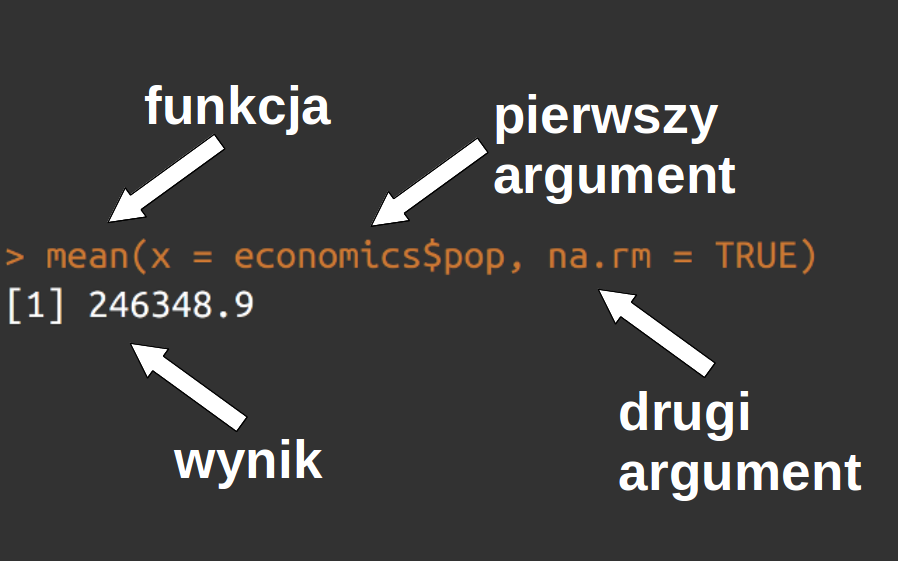
\includegraphics[width=0.8\linewidth]{images/funkcje} 

}

\caption{Przykład struktury funkcji w R.}\label{fig:funstr}
\end{figure}

W efekcie działania funkcji otrzymano wynik - \texttt{246348.9} - który jest średnią wartością w zadanym wektorze.

\hypertarget{wbudowane-funkcje}{%
\section{Wbudowane funkcje}\label{wbudowane-funkcje}}

R posiada wiele wbudowanych funkcji, które znacznie ułatwiają wykonywanie bardziej złożonych operacji.
Pierwsze z funkcji, w tym \texttt{c()}, zostały już poznane w sekcji \ref{dzialania-na-obiektach}.
Ta funkcja pozwala na łączenie kolejnych obiektów rozdzielonych przecinkami.
Poniższy obiekt, \texttt{x} jest w efekcie wektorem zawierającym trzy wartości \texttt{8.2}, \texttt{10.3} oraz \texttt{12.0}.

\begin{Shaded}
\begin{Highlighting}[]
\NormalTok{x =}\StringTok{ }\KeywordTok{c}\NormalTok{(}\FloatTok{8.2}\NormalTok{, }\FloatTok{10.3}\NormalTok{, }\FloatTok{12.0}\NormalTok{)}
\NormalTok{x}
\CommentTok{#> [1]  8.2 10.3 12.0}
\end{Highlighting}
\end{Shaded}

Wyliczenie średniej z tych trzech wartości wymaga ich zsumowania, a następnie podzielenia uzyskanej wartości przez liczbę wartości.

\begin{Shaded}
\begin{Highlighting}[]
\NormalTok{(}\FloatTok{8.2} \OperatorTok{+}\StringTok{ }\FloatTok{10.3} \OperatorTok{+}\StringTok{ }\FloatTok{12.0}\NormalTok{) }\OperatorTok{/}\StringTok{ }\DecValTok{3}
\CommentTok{#> [1] 10.2}
\end{Highlighting}
\end{Shaded}

W przypadku jednak, gdy chcemy dodać czwartą, piątą, itd. wartość należy zmieniać kod w co najmniej dwóch miejscach.
Konieczne jest dodanie nowej wartości do zsumowania, a następnie zmianę wartości określającej liczbę elementów.

Zamiast tych dwóch operacji, można wykonać tylko jedną zmianę w obiekcie \texttt{x}, a następnie przetworzyć go używając funkcji wbudowanych w R - \texttt{sum()} oraz \texttt{length()}.
Pierwsza z nich sumuje wartości z wektora, druga natomiast zwraca liczbę elementów w wektorze.

\begin{Shaded}
\begin{Highlighting}[]
\KeywordTok{sum}\NormalTok{(x) }\OperatorTok{/}\StringTok{ }\KeywordTok{length}\NormalTok{(x)}
\CommentTok{#> [1] 10.2}
\end{Highlighting}
\end{Shaded}

Powyższy kod można też dalej uprościć, poprzez użycie wbudowanej w R funkcji do liczenia średniej - \texttt{mean()}.

\begin{Shaded}
\begin{Highlighting}[]
\KeywordTok{mean}\NormalTok{(x)}
\CommentTok{#> [1] 10.2}
\end{Highlighting}
\end{Shaded}

Jej użycie powoduje, że wystarczy wykonać tylko jedną zmianę w obiekcie \texttt{x}, aby uzyskać poprawny wynik, a dodatkowo napisanie tego obliczenia wymaga napisania znacznie krótszego kodu.

Funkcje można używać w celu wyświetlenia oczekiwanego rezultatu, ale także, aby na podstawie wyniku funkcji tworzyć nowe obiekty, takie jak \texttt{y} poniżej.

\begin{Shaded}
\begin{Highlighting}[]
\NormalTok{y =}\StringTok{ }\KeywordTok{mean}\NormalTok{(x)}
\NormalTok{y}
\CommentTok{#> [1] 10.2}
\end{Highlighting}
\end{Shaded}

\hypertarget{kolejnosc-funkcji}{%
\section{Kolejność wykonywania funkcji}\label{kolejnosc-funkcji}}

Wykonywanie funkcji w R odbywa się linia po linii, od góry do dołu.

\begin{Shaded}
\begin{Highlighting}[]
\NormalTok{a =}\StringTok{ }\DecValTok{4}
\NormalTok{b =}\StringTok{ }\DecValTok{5}
\NormalTok{a2 =}\StringTok{ }\NormalTok{a}\OperatorTok{^}\DecValTok{2}
\NormalTok{b2 =}\StringTok{ }\NormalTok{b}\OperatorTok{^}\DecValTok{2}
\end{Highlighting}
\end{Shaded}

R pozwala na dwa podstawowe sposoby łączenia działania wielu funkcji\footnote{Istnieje też szereg dodatkowych sposobów, wśród których najpopularniejszy polega na używaniu operatora \texttt{\%\textgreater{}\%} z pakietu \textbf{magrittr} \citep{R-magrittr}.}.
Pierwszy z nich polega na tworzeniu pośrednich obiektów jako wyników działania pojedynczych funkcji.

\begin{Shaded}
\begin{Highlighting}[]
\NormalTok{suma_a2b2 =}\StringTok{ }\KeywordTok{sum}\NormalTok{(a2, b2)}
\NormalTok{przekatna =}\StringTok{ }\KeywordTok{sqrt}\NormalTok{(suma_a2b2)}
\NormalTok{przekatna}
\CommentTok{#> [1] 6.4}
\end{Highlighting}
\end{Shaded}

Drugi sposób opiera się o zagnieżdżanie funkcji.
W tej sytuacji najpierw wykonywana jest funkcja w środku, na następnie kolejne funkcje coraz bliżej brzegu.

\begin{Shaded}
\begin{Highlighting}[]
\NormalTok{przekatna =}\StringTok{ }\KeywordTok{sqrt}\NormalTok{(}\KeywordTok{sum}\NormalTok{(a2, b2))}
\NormalTok{przekatna}
\CommentTok{#> [1] 6.4}
\end{Highlighting}
\end{Shaded}

\hypertarget{dokumentacja-funkcji}{%
\section{Dokumentacja funkcji}\label{dokumentacja-funkcji}}

Każda wbudowana funkcja w R posiada swoją dokumentację\footnote{Niektóre zbiory danych również posiadają swoje pliki pomocy.}.
Można ją wyświetlić poprzez dodanie znaku zapytania przed nazwą funkcji, a następnie wykonanie tej linii kodu.

\begin{Shaded}
\begin{Highlighting}[]
\NormalTok{?mean}
\end{Highlighting}
\end{Shaded}

Alternatywnie, w RStudio możliwe jest użycie skrótu F1 gdy kursor znajduje się na nazwie funkcji.

Dokumentacja każdej funkcji, zwana inaczej plikiem pomocy, ma zazwyczaj podobną strukturę.

\begin{itemize}
\tightlist
\item
  W lewym górnym rogu znajduje się nazwa funkcji (\texttt{mean}) oraz nazwa pakietu z którego dana funkcja pochodzi (\texttt{base}).
\item
  Poniżej znajduje się tytuł funkcji oraz jej krótki opis.
\item
  Kolejnym elementem jest budowa funkcji (\emph{Usage}), która skrótowo opisuje z jakich argumentów składa się dana funkcja.
  Np. funkcja \texttt{mean()} przyjmuje argument \texttt{x}, \texttt{trim}, oraz \texttt{na.rm}.
  Dla argumentów \texttt{trim} oraz \texttt{na.rm} są także ustalone ich domyślne wartości.
  Dodatkowo, widoczny jest argument w postaci wielokropka (\texttt{...}).
\item
  Argumenty funkcji są również wypisane oraz skrótowo wyjaśnione.
  Przykładowo, \texttt{x} musi być~obiektem R o typie numerycznym (który łączy typ liczb całkowitych i zmiennoprzecinkowych), logicznym, \texttt{date}, \texttt{date-time}, lub \texttt{time\ interval}.
\item
  Część~\emph{Value} (lub \emph{Details}) opisuje szczegóły wykonywanej funkcji.
\item
  Inne możliwe elementy to np. \emph{References} odnoszący się do artykułu czy książki opisującej daną funkcję lub metodę, czy też~\emph{See also} zawierający odnośniki do innych, podobnych funkcji.
\item
  Jeden z najważniejszych elementów pliku pomocy znajduje się na samym końcu - są to przykłady (\emph{Examples}).
  Jeżeli nie jesteśmy pewni jak dana funkcja działa warto zacząć od skopiowania przykładów a następnie ich wykonania.
\end{itemize}

Czytanie dokumentacji wymaga pewnej wprawy i doświadczenia.
Nie bój się używać innych źródeł pomocy (zobacz sekcję \ref{resources}), jeżeli potrzebujesz zrozumieć działanie danej funkcji.

\hypertarget{pakiety}{%
\section{Pakiety}\label{pakiety}}

Pakiet to zorganizowany zbiór funkcji, który rozszerza możliwości R.
Pakiety oprócz kodu zawierają szereg dodatkowych istotnych elementów, takich jak:

\begin{itemize}
\tightlist
\item
  Informacja o wersji pakietu, jego twórcach, zależnościach, czy licencji
\item
  Dokumentacja
\item
  Przykładowe dane
\item
  Testy kodu
\end{itemize}

Pakiety R mogą być przechowywane i instalowane z wielu miejsc w internecie.
Istnieje jednak jedno centralne repozytorium (CRAN, ang. \emph{the Comprehensive R Archive Network}), które zawiera oficjalne wersje pakietów R.
Wersje deweloperskie (rozwojowe) często można znaleźć~na platformie \href{https://github.com/}{GitHub}.

Do instalacji pakietu w R z repozytorium CRAN służy wbudowana funkcja \texttt{install.packages()}, np:

\begin{Shaded}
\begin{Highlighting}[]
\KeywordTok{install.packages}\NormalTok{(}\StringTok{"stringr"}\NormalTok{) }\CommentTok{#instalacja pakietu stringr}
\end{Highlighting}
\end{Shaded}

Zainstalowanie pakietu w R z platformy GitHub jest możliwe używając, np. funkcji \texttt{install\_github()} z pakietu \textbf{remotes}.

\begin{Shaded}
\begin{Highlighting}[]
\CommentTok{# install.packages("remotes")}
\NormalTok{remotes}\OperatorTok{::}\KeywordTok{install_github}\NormalTok{(}\StringTok{"tidyverse/stringr"}\NormalTok{)}
\end{Highlighting}
\end{Shaded}

W przypadku instalacji pakietu w R z platformy GitHub należy podać nazwę użytkownika lub organizacji, która tworzy ten pakiet (np. powyżej \texttt{tidyverse}) oraz nazwę pakietu (np. powyżej \texttt{stringr}) oddzielone znakiem \texttt{/}.

Podobnie jak instalowanie programów na komputerze - zainstalowanie pakietu odbywa się tylko jeden raz.

\begin{rmdinfo}
Istnieją dwa główne formy, w których rozpowszechniane są pakiety R - postać źródłowa (ang. \emph{source packages}) i postać binarna (ang. \emph{binary packages}).
Postać źródłowa zawiera kod źródłowy pakietu, który musi zostać następnie skompilowany na komputerze użytkownika.
Skompilowanie pakietu na podstawie kodu źródłowego może wymagać posiadania odpowiednich bibliotek na komputerze, np. \href{https://cran.r-project.org/bin/windows/Rtools/}{Rtools} dla systemu Windows czy też narzędzia Xcode dla Mac OS.
Dodatkowo, instalacja w ten sposób zabiera więcej czasu.
Postać binarna została już wcześniej skompilowana na zewnętrznym komputerze (np. w repozytorium CRAN)
Jest ona dostępna dla systemów Windows i Mac OS.
Niestety, nie wszystkie pakiety (lub ich wersje) posiadają postać binarną i wymagana jest ich kompilacja.
\end{rmdinfo}

Użycie wybranego pakietu wymaga dołączenia go do R za pomocą funkcji \texttt{library()}.
Dołączenie wybranych pakietów do R robimy po każdym uruchomieniu R.

\begin{Shaded}
\begin{Highlighting}[]
\KeywordTok{library}\NormalTok{(stringr)}
\end{Highlighting}
\end{Shaded}

W przypadku, gdy chcemy użyć zewnętrznej funkcji, ale nie dołączyliśmy odpowiedniego pakietu, pojawi się~błąd o treści \texttt{could\ not\ find\ function\ "nazwa\_funkcji"}.

\begin{Shaded}
\begin{Highlighting}[]
\KeywordTok{str_sub}\NormalTok{(}\StringTok{"chronologia"}\NormalTok{, }\DataTypeTok{start =} \DecValTok{1}\NormalTok{, }\DataTypeTok{end =} \DecValTok{6}\NormalTok{)}
\CommentTok{#> Error in str_sub("chronologia", start = 1, end = 6) : }
\CommentTok{#>  could not find function "str_sub"}
\end{Highlighting}
\end{Shaded}

Istnieją dwa możliwe rozwiązania powyższego problemu.
Po pierwsze możliwe jest dołączenie pakietu poprzez \texttt{library(stringr)}.
Po drugie można bezpośrednio zdefiniować z jakiego pakietu pochodzi konkretna funkcja używając nazwy pakietu i operatora \texttt{::}.

\begin{Shaded}
\begin{Highlighting}[]
\NormalTok{stringr}\OperatorTok{::}\KeywordTok{str_sub}\NormalTok{(}\StringTok{"chronologia"}\NormalTok{, }\DataTypeTok{start =} \DecValTok{1}\NormalTok{, }\DataTypeTok{end =} \DecValTok{6}\NormalTok{)}
\CommentTok{#> [1] "chrono"}
\end{Highlighting}
\end{Shaded}

\begin{rmdinfo}
Operator \texttt{::} może być też pomocny w przypadku, gdy kilka pakietów ma funkcję o tej samej nazwie.
Wówczas, aby kod został poprawnie wykonany, warto podać nie tylko nazwę funkcji ale też nazwę pakietu z jakiego ona pochodzi.
\end{rmdinfo}

\hypertarget{algorytmy}{%
\section{Algorytmy}\label{algorytmy}}

Algorytm to zbiór kroków prowadzących do uzyskania określonego celu.
Algorytmy można porównać do przepisu kucharskiego, w którym opisany jest szereg czynności aby uzyskać konkretną potrawę.
Podobnie jak w przepisie kucharskim, algorytmy wymagają posiadania odpowiednich składników - danych wejściowych w o pewnej strukturze.

Tworzenie nowych algorytmów często zaczyna się od narysowania schematu procedury działania lub też pseudokodu.
Kolejnym krokiem jest zapisanie tego algorytmu w wybranym języku lub językach programowania w formie skryptu (sekcja \ref{tworzenie-skryptow}) lub funkcji (sekcja \ref{budowanie-funkcji}).

\hypertarget{tworzenie-skryptow}{%
\section{Tworzenie skryptów}\label{tworzenie-skryptow}}

Skrypt w R to plik testowy z rozszerzeniem \texttt{.R}, który zawiera szereg linii kodu w celu uzyskania konkretnego efektu.
Może on zawierać zaledwie kilka jak i setki linii kodu w zależności od złożoności postawionego problemu.
Zobaczmy jak wyglądają skrypty na prostym przykładzie - przeliczania wartości temperatury w stopniach ze skali Fahrenheita na skalę Celsjusza.
Otrzymaliśmy informację, że w ``mieście A'' temperatura w stopniach Fahrenheita wynosi 75.

\begin{Shaded}
\begin{Highlighting}[]
\NormalTok{miasto_a_f =}\StringTok{ }\DecValTok{75}
\end{Highlighting}
\end{Shaded}

Pierwszym naszym krokiem powinno być~dowiedzenie się jaka jest relacja pomiędzy skalą Fahrenheita na skalą Celsjusza.

\[T_{Celsjusz} = \frac{T_{Fahrenheit} - 32}{1.8}\]

Następnie powyższy wzór można przepisać do postaci kodu w języku R oraz podstawić do niego wartość temperatury w stopniach Fahrenheita w mieście A.
Ostatnim etapem jest wyświetlenie uzyskanego wyniku - temperatura w mieście A wynosi ok. 24 stopnie Celsjusza.

\begin{Shaded}
\begin{Highlighting}[]
\NormalTok{miasto_a_c =}\StringTok{ }\NormalTok{(miasto_a_f }\OperatorTok{-}\StringTok{ }\DecValTok{32}\NormalTok{) }\OperatorTok{/}\StringTok{ }\FloatTok{1.8}
\NormalTok{miasto_a_c}
\CommentTok{#> [1] 23.9}
\end{Highlighting}
\end{Shaded}

Powyższe kroki można również zapisać do pliku tekstowego.

\begin{Shaded}
\begin{Highlighting}[]
\CommentTok{# plik przeliczanie-temp.R}
\NormalTok{miasto_a_f =}\StringTok{ }\DecValTok{75}
\NormalTok{miasto_a_c =}\StringTok{ }\NormalTok{(miasto_a_f }\OperatorTok{-}\StringTok{ }\DecValTok{32}\NormalTok{) }\OperatorTok{/}\StringTok{ }\FloatTok{1.8}
\NormalTok{miasto_a_c}
\end{Highlighting}
\end{Shaded}

Co można zrobić jeżeli mamy więcej podobnych pomiarów, które chcemy wykonać?
Najprostszą opcją jest użycie kopiuj/wklej i powielenie tego samego kodu, a później naniesienie małych zmian, np. nazw obiektów.

\begin{Shaded}
\begin{Highlighting}[]
\NormalTok{miasto_a_f =}\StringTok{ }\DecValTok{75}
\NormalTok{miasto_b_f =}\StringTok{ }\DecValTok{110}
\NormalTok{miasto_c_f =}\StringTok{ }\DecValTok{0}
\NormalTok{miasto_a_c =}\StringTok{ }\NormalTok{(miasto_a_f }\OperatorTok{-}\StringTok{ }\DecValTok{32}\NormalTok{) }\OperatorTok{/}\StringTok{ }\FloatTok{1.8}
\NormalTok{miasto_b_c =}\StringTok{ }\NormalTok{(miasto_b_f }\OperatorTok{-}\StringTok{ }\DecValTok{32}\NormalTok{) }\OperatorTok{/}\StringTok{ }\FloatTok{1.8}
\NormalTok{miasto_c_c =}\StringTok{ }\NormalTok{(miasto_c_f }\OperatorTok{-}\StringTok{ }\DecValTok{32}\NormalTok{) }\OperatorTok{/}\StringTok{ }\FloatTok{1.8}
\end{Highlighting}
\end{Shaded}

Powyższe podejście jest poprawne, ale ma ono kilka wad:

\begin{itemize}
\tightlist
\item
  Łatwo jest o popełnienie jakiegoś prostego błędu lub literówki podczas adaptacji kodu (np. można zapomnieć zmienić nazwę jakiejś zmiennej).
\item
  Jeżeli obliczenia zajmują więcej niż kilka linii kodu - wówczas kopiowanie go znacznie powiększa tworzony skrypt i utrudnia jego czytelność.
\item
  Poprawienie kodu w przypadku zauważenia błędu w procedurze obliczeniowej jest czasochłonne.
\end{itemize}

To podejście jest też niezgodne z jedną z najważniejszych reguł w programowaniu - regułą DRY (Nie powtarzaj się, ang. \emph{Don't Repeat Yourself}).
Zamiast tworzenia skryptu w oparciu o kopiuj/wklej lepiej pomyśleć nad zbudowaniem odpowiedniej funkcji\footnote{\citet{wickham2016r} radzą tworzyć nowe funkcje, gdy ten sam kod powtarza się~co najmniej trzy razy.}.

\hypertarget{budowanie-funkcji}{%
\section{Budowanie funkcji}\label{budowanie-funkcji}}

Funkcje pozwalają na automatyzację często używanych obliczeń.
Formalnie funkcje składają się z trzech elementów: listy argumentów (ang. \emph{formals}), ciała funkcji (ang. \emph{body}) oraz środowiska (ang. \emph{environment}).
Pierwsze dwa elementy ustala twórca funkcji, natomiast środowisko jest określane na podstawie tego, gdzie dana funkcja została zdefiniowana.
Dodatkowo każda funkcja ma swoją nazwę.

\begin{Shaded}
\begin{Highlighting}[]
\NormalTok{moja_funkcja =}\StringTok{ }\ControlFlowTok{function}\NormalTok{(x, y, z)\{}
\NormalTok{  pod =}\StringTok{ }\NormalTok{y }\OperatorTok{/}\StringTok{ }\NormalTok{z}
\NormalTok{  wynik =}\StringTok{ }\NormalTok{x }\OperatorTok{*}\StringTok{ }\NormalTok{pod}
\NormalTok{  wynik}
\NormalTok{\}}
\end{Highlighting}
\end{Shaded}

Lista argumentów wymienia obiekty wejściowe funkcji.

\begin{Shaded}
\begin{Highlighting}[]
\KeywordTok{formals}\NormalTok{(moja_funkcja)}
\CommentTok{#> $x}
\CommentTok{#> }
\CommentTok{#> }
\CommentTok{#> $y}
\CommentTok{#> }
\CommentTok{#> }
\CommentTok{#> $z}
\end{Highlighting}
\end{Shaded}

Ciało zawiera kod danej funkcji.

\begin{Shaded}
\begin{Highlighting}[]
\KeywordTok{body}\NormalTok{(moja_funkcja)}
\CommentTok{#> \{}
\CommentTok{#>     pod = y/z}
\CommentTok{#>     wynik = x * pod}
\CommentTok{#>     wynik}
\CommentTok{#> \}}
\end{Highlighting}
\end{Shaded}

Środowisko określa, gdzie dana funkcja jest zlokalizowana.

\begin{Shaded}
\begin{Highlighting}[]
\KeywordTok{environment}\NormalTok{(moja_funkcja)}
\CommentTok{#> <environment: R_GlobalEnv>}
\end{Highlighting}
\end{Shaded}

Przykładowa funkcja odpowiadająca problemowi z poprzedniej sekcji może wyglądać w poniższy sposób:

\begin{Shaded}
\begin{Highlighting}[]
\NormalTok{konwersja_temp =}\StringTok{ }\ControlFlowTok{function}\NormalTok{(temperatura_f)\{}
\NormalTok{    (temperatura_f }\OperatorTok{-}\StringTok{ }\DecValTok{32}\NormalTok{) }\OperatorTok{/}\StringTok{ }\FloatTok{1.8}
\NormalTok{\}}
\end{Highlighting}
\end{Shaded}

Nowa funkcja nazywa się \texttt{konwersja\_temp()} oraz posiada tylko jeden argument \texttt{temperatura\_f}.
Ciało funkcji zawiera natomiast wzór potrzebny do obliczeń przepisany do R.
Ważne jest to, że obiekt użyty wewnątrz funkcji (\texttt{temperatura\_f}) jest taki sam jak wejściowy argument.

Po stworzeniu funkcji warto sprawdzić czy jej działanie odpowiada naszym oczekiwaniom.

\begin{Shaded}
\begin{Highlighting}[]
\KeywordTok{konwersja_temp}\NormalTok{(}\DecValTok{75}\NormalTok{)}
\CommentTok{#> [1] 23.9}
\KeywordTok{konwersja_temp}\NormalTok{(}\DecValTok{110}\NormalTok{)}
\CommentTok{#> [1] 43.3}
\KeywordTok{konwersja_temp}\NormalTok{(}\DecValTok{0}\NormalTok{)}
\CommentTok{#> [1] -17.8}
\KeywordTok{konwersja_temp}\NormalTok{(}\KeywordTok{c}\NormalTok{(}\DecValTok{0}\NormalTok{, }\DecValTok{75}\NormalTok{, }\DecValTok{110}\NormalTok{))}
\CommentTok{#> [1] -17.8  23.9  43.3}
\end{Highlighting}
\end{Shaded}

\hypertarget{komunikaty}{%
\section{Komunikaty}\label{komunikaty}}

Oprócz wyniku danej operacji R może wyświetlić kilka rodzajów komunikatów.
Trzy podstawowe z nich to:

\begin{enumerate}
\def\labelenumi{\arabic{enumi}.}
\tightlist
\item
  Błędy (ang. \emph{errors})
\item
  Ostrzeżenia (ang. \emph{warnings})
\item
  Wiadomości (ang. \emph{messages})
\end{enumerate}

Błędy oznaczają, że wykonanie danej funkcji nie może być kontynuowane i przerwane jest jej działanie.
Przykładowo, w poniższym kodzie podjęta została próba wyliczenia logarytmu naturalnego z tekstu \texttt{"abecadło"}.
Takie obliczenie nie jest możliwe, w efekcie pojawił się~komunikat błędu a kod nie został wykonany.

\begin{Shaded}
\begin{Highlighting}[]
\KeywordTok{log}\NormalTok{(}\StringTok{"abecadło"}\NormalTok{)}
\CommentTok{#> Error in log("abecadło"): non-numeric argument to mathematical function}
\end{Highlighting}
\end{Shaded}

Ostrzeżenia zazwyczaj występują kiedy nastąpił jakiś~problem z wykonaniem funkcji, ale jej działanie mogło być dokończone.
Często sugerują one użytkownikowi, aby dokładnie przyjrzał się wykonywanej funkcji i upewnił się czy na pewno ustala on odpowiednie wartości dla argumentów funkcji.
Poniżej została podjęta próba wyliczenia logarytmu naturalnego dla wartości ujemnej.
W efekcie pojawił się komunikat błędu, który mówi, że w wyniku zostały stworzone wartości \texttt{NaN} (ang. \emph{Not a Number}).

\begin{Shaded}
\begin{Highlighting}[]
\KeywordTok{log}\NormalTok{(}\OperatorTok{-}\DecValTok{1}\NormalTok{)}
\CommentTok{#> Warning in log(-1): NaNs produced}
\CommentTok{#> [1] NaN}
\end{Highlighting}
\end{Shaded}

Wiadomości pojawiają się, aby przekazać użytkownikowi jakąś informację.

\begin{Shaded}
\begin{Highlighting}[]
\KeywordTok{inna_funkcja}\NormalTok{(}\DecValTok{15}\NormalTok{)}
\CommentTok{#> Chcę ciebie o czymś poinformować.}
\CommentTok{#> [1] 2.71}
\end{Highlighting}
\end{Shaded}

Opis tworzenia komunikatów błędu, ostrzeżenia i wiadomości można znaleźć~w rozdziale \ref{zlozone-funkcje}.

\hypertarget{zadania}{%
\section{Zadania}\label{zadania}}

\begin{enumerate}
\def\labelenumi{\arabic{enumi})}
\tightlist
\item
  Zobacz jak wygląda plik pomocy funkcji \texttt{mean()}.
  Wykonaj zawarte w nim przykłady.
  Co przedstawiają uzyskane wyniki?
\item
  Zainstaluj pakiet \textbf{magrittr}.
  Spróbuj użyć operatora \texttt{\%\textgreater{}\%} z tego pakietu na przykładzie z sekcji \ref{kolejnosc-funkcji} dotyczącym wyliczania przekątnej prostokąta.
\item
  Stwórz nowy plik skryptu R nazywający się \texttt{01\_zadania-funkcje.R}.
  W tym pliku, stwórz nowy obiekt \texttt{poznan}, który przyjmuje wartość~\texttt{8.4}, napisz przeliczenie wartości tego obiektu ze stopni Celsjusza na stopnie Fahrenheita, a następnie wyświetl uzyskany wynik.
  Uwaga: pamiętaj o ustawieniu odpowiedniego kodowania znaków dla tego nowego pliku.
\item
  Stwórz nową funkcję, która służy do przeliczania wartości ze stopni Celsjusza na stopnie Fahrenheita.
  Jak nazwiesz taką funkcję?
\item
  Stwórz nową funkcję, która służy do przeliczania wartości z mil lądowych na kilometry.
  Jak nazwiesz taką funkcję?
\item
  Stwórz nową funkcję, która służy do przeliczania wartości z metrów na sekundę na kilometry na godzinę.
  Jak nazwiesz taką funkcję?
\item
  Stwórz nową funkcję, która służy do przeliczania wartości z metrów na sekundę na mile lądowe na godzinę.
  Jak nazwiesz taką funkcję?
\item
  Stwórz nową funkcję, która służy do wyliczania pola trapezu na podstawie długości podstaw oraz wysokości trapezu.
  Jak nazwiesz taką funkcję?
\item
  Wykonaj poniższy kod.
  Co oznacza uzyskany wynik?
\end{enumerate}

\begin{Shaded}
\begin{Highlighting}[]
\KeywordTok{mean}\NormalTok{()}
\end{Highlighting}
\end{Shaded}

\begin{enumerate}
\def\labelenumi{\arabic{enumi})}
\setcounter{enumi}{9}
\tightlist
\item
  Wykonaj poniższy kod.
  Co oznacza uzyskany wynik?
\end{enumerate}

\begin{Shaded}
\begin{Highlighting}[]
\KeywordTok{mean}\NormalTok{(}\StringTok{"abecadło"}\NormalTok{)}
\end{Highlighting}
\end{Shaded}

\begin{enumerate}
\def\labelenumi{\arabic{enumi})}
\setcounter{enumi}{10}
\tightlist
\item
  Wykonaj poniższy kod.
  Co oznacza uzyskany wynik?
\end{enumerate}

\begin{Shaded}
\begin{Highlighting}[]
\KeywordTok{mean}\NormalTok{(}\KeywordTok{sqrt}\NormalTok{())}
\end{Highlighting}
\end{Shaded}

\begin{enumerate}
\def\labelenumi{\arabic{enumi})}
\setcounter{enumi}{11}
\tightlist
\item
  Wykonaj poniższy kod.
  Co oznacza uzyskany wynik?
\end{enumerate}

\begin{Shaded}
\begin{Highlighting}[]
\KeywordTok{str_length}\NormalTok{(}\StringTok{"abecadło"}\NormalTok{)}
\end{Highlighting}
\end{Shaded}

\begin{enumerate}
\def\labelenumi{\arabic{enumi})}
\setcounter{enumi}{12}
\tightlist
\item
  Wykonaj poniższy kod.
  Co oznacza uzyskany wynik?
\end{enumerate}

\begin{Shaded}
\begin{Highlighting}[]
\NormalTok{u =}\StringTok{ }\DecValTok{2}
\NormalTok{z =}\StringTok{ }\DecValTok{3} \OperatorTok{+}\StringTok{ }\NormalTok{v}
\NormalTok{v =}\StringTok{ }\DecValTok{7}
\end{Highlighting}
\end{Shaded}

\hypertarget{warunki}{%
\chapter{Wyrażenia warunkowe}\label{warunki}}

Języki programowania opierają się o dwa podstawowe narzędzia pozwalające na sterowanie przepływem operacji.
Są to wyrażenia warunkowe oraz pętle.
Wyrażenia warunkowe są głównym tematem tego rozdziału, natomiast pętle oraz ich alternatywy są omówione w rozdziale \ref{petle}.
Celem wyrażeń warunkowych jest wykonywanie różnego zadania w zależności od danych wejściowych.

\hypertarget{warunki-1}{%
\section{Warunki}\label{warunki-1}}

Wyrażenie \texttt{if} opiera się o spełnienie (lub niespełnienie) danego warunku.
Jeżeli dany warunek jest spełniony, kod wewnątrz wyrażenia \texttt{if()} jest wykonywany.
W przeciwnym razie cały blok kodu jest pomijany.

\begin{Shaded}
\begin{Highlighting}[]
\ControlFlowTok{if}\NormalTok{ (warunek)\{}
\NormalTok{  jeżeli warunek spełniony to wykonaj operację}
\NormalTok{\}}
\end{Highlighting}
\end{Shaded}

Wyrażenie \texttt{if} oczekuje, że warunek jest wektorem logicznym o długości jeden, tj. takim który przyjmuje wartość \texttt{TRUE} lub \texttt{FALSE}.
Istnieje szereg sposób uzyskania wektora logicznego w R, jednym z nich jest zastosowanie porównania wartości.

W poniższym przykładzie wyrażenie \texttt{if()} sprawdza czy wartość~obiektu \texttt{temperatura} jest wyższa niż 0.
W przypadku, gdy ten warunek jest spełniony (czyli przyjmuje \texttt{TRUE}), wyświetlany jest tekst \texttt{"Dodatnia"}.

\begin{Shaded}
\begin{Highlighting}[]
\NormalTok{temperatura =}\StringTok{ }\FloatTok{5.4}
\ControlFlowTok{if}\NormalTok{ (temperatura }\OperatorTok{>}\StringTok{ }\DecValTok{0}\NormalTok{) \{}
  \StringTok{"Dodatnia"}
\NormalTok{\}}
\CommentTok{#> [1] "Dodatnia"}
\end{Highlighting}
\end{Shaded}

W przeciwnym razie, gdy warunek nie jest spełniony (czyli ma wartość \texttt{FALSE}), kod wewnątrz warunku nie jest wykonywany.

\begin{Shaded}
\begin{Highlighting}[]
\NormalTok{temperatura =}\StringTok{ }\DecValTok{-11}
\ControlFlowTok{if}\NormalTok{ (temperatura }\OperatorTok{>}\StringTok{ }\DecValTok{0}\NormalTok{) \{}
  \StringTok{"Dodatnia"}
\NormalTok{\}}
\end{Highlighting}
\end{Shaded}

\begin{rmdinfo}
Warunek \texttt{if} można też tworzyć w uproszczonej formie:

\texttt{if\ (warunek)\ spelniony\ else\ niespelniony}
\end{rmdinfo}

\hypertarget{warunki-zagnieux17cdux17cone}{%
\section{Warunki zagnieżdżone}\label{warunki-zagnieux17cdux17cone}}

Działanie wyrażenia \texttt{if} może być połączone z dodatkowymi wyrażeniami \texttt{else\ if} oraz \texttt{else}.
Te dwa wyrażenia wymagają najpierw wywołania wyrażenia \texttt{if()}.
Jeżeli warunek w wyrażeniu \texttt{if()} jest równy \texttt{TRUE} to wykonywany jest kod w nim zawarty, a następnie obliczenie jest kończone.
W przypadku, gdy wyrażenie \texttt{if()} otrzyma wartość \texttt{FALSE}, to kod w nim zawarty nie jest wykonywany, a następuje przejście do kolejnego wyrażenia, np. \texttt{else\ if()} w poniższym przypadku.

\begin{Shaded}
\begin{Highlighting}[]
\NormalTok{temperatura =}\StringTok{ }\FloatTok{8.8}
\ControlFlowTok{if}\NormalTok{ (temperatura }\OperatorTok{>}\StringTok{ }\DecValTok{0}\NormalTok{) \{}
  \StringTok{"Dodatnia"}
\NormalTok{\} }\ControlFlowTok{else} \ControlFlowTok{if}\NormalTok{ (temperatura }\OperatorTok{<}\StringTok{ }\DecValTok{0}\NormalTok{) \{}
  \StringTok{"Ujemna"}
\NormalTok{\} }\ControlFlowTok{else}\NormalTok{ \{}
  \StringTok{"Zero"}
\NormalTok{\}}
\CommentTok{#> [1] "Dodatnia"}
\end{Highlighting}
\end{Shaded}

Wyrażenie \texttt{else\ if()} różni się od \texttt{else} tym, że wymaga ono określenia jaki warunek ma być spełniony.
W przypadku \texttt{else} wyliczane są wszystkie przypadki, które nie spełniają wcześniejszych warunków.

\hypertarget{operatory-poruxf3wnania}{%
\section{Operatory porównania}\label{operatory-poruxf3wnania}}

W tabeli \ref{tab:operators} można znaleźć listę podstawowych operatorów porównania.
Ich celem jest sprawdzanie pewnego warunku i zwrócenie wartości \texttt{TRUE} lub \texttt{FALSE}.

\begin{table}

\caption{\label{tab:operators}Operatory porównania.}
\centering
\begin{tabular}[t]{ll}
\toprule
Operator & Wyjaśnienie\\
\midrule
== & Równy\\
!= & Nie równy\\
\%in\% & Zawiera się w\\
>, < & Większy/Mniejszy niż\\
>=, <= & Większy/Mniejszy niż lub równy\\
\bottomrule
\end{tabular}
\end{table}

Wyrażenie \texttt{if()} oczekuje wektora logicznego o długości jeden.
Często jednak efektem porównania może być wektor o większej długości.
Przykładowo, porównanie operatorem \texttt{==} daje w wyniku wektor o długości trzy, a porównanie z użyciem \texttt{\%in\%} skutkuje wektorem o długości jeden.

\begin{Shaded}
\begin{Highlighting}[]
\NormalTok{x =}\StringTok{ }\DecValTok{1}
\NormalTok{y =}\StringTok{ }\KeywordTok{c}\NormalTok{(}\DecValTok{1}\NormalTok{, }\DecValTok{2}\NormalTok{, }\DecValTok{3}\NormalTok{)}
\NormalTok{x }\OperatorTok{==}\StringTok{ }\NormalTok{y}
\CommentTok{#> [1]  TRUE FALSE FALSE}
\NormalTok{x }\OperatorTok\StringTok{ }\NormalTok{y}
\CommentTok{#> [1] TRUE}
\end{Highlighting}
\end{Shaded}

Sterowanie tym, żeby uzyskany wynik miał oczekiwaną długość jeden może się odbywać też z pomocą operatorów logicznych i funkcji pomocniczych (tabela \ref{tab:operators2}).

\begin{table}

\caption{\label{tab:operators2}Operatory logiczne i funkcje pomocniczne.}
\centering
\begin{tabular}[t]{ll}
\toprule
Operator & Wyjaśnienie\\
\midrule
! & Negacja (nie)\\
\&\& & Koniunkcja (i)\\
|| & Alternatywa (lub)\\
all & Wszystkie\\
any & Którykolwiek\\
\bottomrule
\end{tabular}
\end{table}

Pozwalają one na sprawdzenie czy wszystkie (\texttt{all()}) lub którykolwiek (\texttt{any()}) z elementów obiektu przyjmuje wartość~\texttt{TRUE}.

\begin{Shaded}
\begin{Highlighting}[]
\NormalTok{x =}\StringTok{ }\DecValTok{1}
\NormalTok{y =}\StringTok{ }\KeywordTok{c}\NormalTok{(}\DecValTok{1}\NormalTok{, }\DecValTok{2}\NormalTok{, }\DecValTok{3}\NormalTok{)}
\KeywordTok{all}\NormalTok{(x }\OperatorTok{==}\StringTok{ }\NormalTok{y)}
\CommentTok{#> [1] FALSE}
\KeywordTok{any}\NormalTok{(x }\OperatorTok{==}\StringTok{ }\NormalTok{y)}
\CommentTok{#> [1] TRUE}
\end{Highlighting}
\end{Shaded}

Możliwe jest też łączenie bardziej złożonych zapytań używając operatora ``i'' (\texttt{\&\&}) oraz operatora ``lub'' (\texttt{\textbar{}\textbar{}}).

\begin{Shaded}
\begin{Highlighting}[]
\NormalTok{x =}\StringTok{ }\DecValTok{1}
\NormalTok{y =}\StringTok{ }\KeywordTok{c}\NormalTok{(}\DecValTok{1}\NormalTok{, }\DecValTok{2}\NormalTok{, }\DecValTok{3}\NormalTok{)}
\NormalTok{z =}\StringTok{ }\DecValTok{4}
\NormalTok{(x }\OperatorTok\StringTok{ }\NormalTok{y) }\OperatorTok{||}\StringTok{ }\OperatorTok{!}\NormalTok{(z }\OperatorTok\StringTok{ }\NormalTok{y)}
\CommentTok{#> [1] TRUE}
\end{Highlighting}
\end{Shaded}

Powyżej nastąpiło sprawdzenie czy element z obiektu \texttt{x} znajduje się w obiekcie \texttt{y}, a następnie czy element z obiektu \texttt{z} nie znajduje się w obiekcie \texttt{y}.
Po wykonaniu ich sprawdzeń nastąpiło ich połączenie używając operatora \texttt{\textbar{}\textbar{}}, który daje wartość~\texttt{TRUE}, gdy chociaż jedno z zapytań jest prawdziwe.

\begin{rmdinfo}
W R istnieją dwa dodatkowe operatory logiczne \texttt{\&} i \texttt{\textbar{}}, które są zwektoryzowaną wersją operatorów \texttt{\&\&} i \texttt{\textbar{}\textbar{}}.
Pierwsze dwa porównują wszystkie elementy zadanych wektorów i ich wynikiem może być wektor o długości większej niż 1.
Operatory \texttt{\&\&} i \texttt{\textbar{}\textbar{}} porównują tylko pierwszy element każdego wektora, a w efekcie zawsze zwracają tylko jedną wartość.
Dodatkowo, to one są zazwyczaj używane w wyrażeniach warunkowych.
\end{rmdinfo}

\hypertarget{wwwf}{%
\section{Wyrażenia warunkowe w funkcjach}\label{wwwf}}

Wyrażenia warunkowe są często używanym elementem przy tworzeniu funkcji.
Pozwalają one na nie tylko na określanie tego w jaki sposób dana funkcja zadziała, ale też~pełnią rolę w sprawdzaniu czy do funkcji zostały wprowadzone poprawne argumenty.

Celem poniższej funkcji \texttt{pogoda()} jest wyświetlenie pewnego tekstu w zależności od podanej wartości argumentu \texttt{temperatura}.
Pierwszym warunkiem, który można sprawdzić jest określenie czy użytkownik wprowadził do funkcji w postaci argumentu oczekiwany typ danych (więcej o typach danych można dowiedzieć się w rozdziale \ref{proste-obiekty}).
W tym przypadku typ numeryczny jest oczekiwany, co można sprawdzić używając funkcji \texttt{is.numeric()}, która zwraca \texttt{TRUE} dla danych numerycznych i \texttt{FALSE} dla każdych innych.

\begin{Shaded}
\begin{Highlighting}[]
\NormalTok{pogoda =}\StringTok{ }\ControlFlowTok{function}\NormalTok{(temperatura)\{}
  \ControlFlowTok{if}\NormalTok{ (}\KeywordTok{is.numeric}\NormalTok{(temperatura))\{}
    \KeywordTok{cat}\NormalTok{(}\KeywordTok{paste}\NormalTok{(}\StringTok{"Dzisiaj jest"}\NormalTok{, temperatura, }\StringTok{"stopni Celsjusza."}\NormalTok{))}
\NormalTok{  \}}
\NormalTok{\}}
\KeywordTok{pogoda}\NormalTok{(}\DecValTok{10}\NormalTok{)}
\CommentTok{#> Dzisiaj jest 10 stopni Celsjusza.}
\KeywordTok{pogoda}\NormalTok{(}\OperatorTok{-}\DecValTok{20}\NormalTok{)}
\CommentTok{#> Dzisiaj jest -20 stopni Celsjusza.}
\KeywordTok{pogoda}\NormalTok{(}\StringTok{"nie wiem"}\NormalTok{)}
\end{Highlighting}
\end{Shaded}

Efekt działania powyższej funkcji jest teraz zależy od wejściowego typu danych - jeżeli podana jest wartość numeryczna zwracany jest tekst, a jeżeli ten warunek nie jest spełniony to nic się~nie dzieje.

Warto, aby tworzona funkcja obsługiwała najczęściej potencjalnie używane rodzaje danych wejściowych.
W tym przypadku, warto dodać wyrażenie \texttt{else}, którego efektem jest kolejny tekst sugerujący, że funkcja została wykonana, ale w inny sposób.

\begin{Shaded}
\begin{Highlighting}[]
\NormalTok{pogoda =}\StringTok{ }\ControlFlowTok{function}\NormalTok{(temperatura)\{}
  \ControlFlowTok{if}\NormalTok{ (}\KeywordTok{is.numeric}\NormalTok{(temperatura))\{}
    \KeywordTok{cat}\NormalTok{(}\KeywordTok{paste}\NormalTok{(}\StringTok{"Dzisiaj jest"}\NormalTok{, temperatura, }\StringTok{"stopni Celsjusza."}\NormalTok{))}
\NormalTok{  \} }\ControlFlowTok{else}\NormalTok{ \{}
    \KeywordTok{cat}\NormalTok{(}\StringTok{"Dzisiaj nie mamy pomiarów temperatury."}\NormalTok{)}
\NormalTok{  \}}
\NormalTok{\}}
\KeywordTok{pogoda}\NormalTok{(}\DecValTok{10}\NormalTok{)}
\CommentTok{#> Dzisiaj jest 10 stopni Celsjusza.}
\KeywordTok{pogoda}\NormalTok{(}\OperatorTok{-}\DecValTok{20}\NormalTok{)}
\CommentTok{#> Dzisiaj jest -20 stopni Celsjusza.}
\KeywordTok{pogoda}\NormalTok{(}\StringTok{"nie wiem"}\NormalTok{)}
\CommentTok{#> Dzisiaj nie mamy pomiarów temperatury.}
\end{Highlighting}
\end{Shaded}

Wyrażenia warunkowe można też wielokrotnie zagnieżdżać wewnątrz zdefiniowanej funkcji.

\begin{Shaded}
\begin{Highlighting}[]
\NormalTok{pogoda =}\StringTok{ }\ControlFlowTok{function}\NormalTok{(temperatura)\{}
  \ControlFlowTok{if}\NormalTok{ (}\KeywordTok{is.numeric}\NormalTok{(temperatura))\{}
    \KeywordTok{cat}\NormalTok{(}\KeywordTok{paste}\NormalTok{(}\StringTok{"Dzisiaj jest"}\NormalTok{, temperatura, }\StringTok{"stopni Celsjusza.}\CharTok{\textbackslash{}n}\StringTok{"}\NormalTok{))}
    \ControlFlowTok{if}\NormalTok{ (temperatura }\OperatorTok{<}\StringTok{ }\DecValTok{5}\NormalTok{)\{}
      \KeywordTok{cat}\NormalTok{(}\StringTok{"Ubierz się ciepło!"}\NormalTok{)}
\NormalTok{    \}}
\NormalTok{  \} }\ControlFlowTok{else}\NormalTok{ \{}
    \KeywordTok{cat}\NormalTok{(}\StringTok{"Dzisiaj nie mamy pomiarów temperatury."}\NormalTok{)}
\NormalTok{  \}}
\NormalTok{\}}
\KeywordTok{pogoda}\NormalTok{(}\DecValTok{10}\NormalTok{)}
\CommentTok{#> Dzisiaj jest 10 stopni Celsjusza.}
\KeywordTok{pogoda}\NormalTok{(}\OperatorTok{-}\DecValTok{20}\NormalTok{)}
\CommentTok{#> Dzisiaj jest -20 stopni Celsjusza.}
\CommentTok{#> Ubierz się ciepło!}
\KeywordTok{pogoda}\NormalTok{(}\StringTok{"nie wiem"}\NormalTok{)}
\CommentTok{#> Dzisiaj nie mamy pomiarów temperatury.}
\end{Highlighting}
\end{Shaded}

Przykładowo, powyżej komunikat \texttt{"Ubierz\ się\ ciepło!"} jest wyświetlany w momencie, gdy spełnione zostaną dwa warunki - najpierw wejściowy obiekt \texttt{temperatura} musi być typu numerycznego, a następnie wartość tego obiektu musi być niższa niż 5.

\hypertarget{zadania}{%
\section{Zadania}\label{zadania}}

\begin{enumerate}
\def\labelenumi{\arabic{enumi})}
\tightlist
\item
  Spójrz na poniższe przykłady, ale ich nie wykonuj.
  Co będzie wynikiem działania każdego z tych przykładów?
\end{enumerate}

\begin{Shaded}
\begin{Highlighting}[]
\NormalTok{liczby =}\StringTok{ }\KeywordTok{c}\NormalTok{(}\DecValTok{1}\NormalTok{, }\DecValTok{2}\NormalTok{)}
\NormalTok{liczby }\OperatorTok{==}\StringTok{ }\DecValTok{1}          \CommentTok{#1}
\NormalTok{liczby }\OperatorTok{!=}\StringTok{ }\DecValTok{1}          \CommentTok{#2}
\NormalTok{liczby }\OperatorTok\StringTok{ }\DecValTok{1}        \CommentTok{#3}
\KeywordTok{all}\NormalTok{(liczby }\OperatorTok\StringTok{ }\DecValTok{1}\NormalTok{)   }\CommentTok{#4}
\KeywordTok{any}\NormalTok{(liczby }\OperatorTok\StringTok{ }\DecValTok{1}\NormalTok{)   }\CommentTok{#5}
\end{Highlighting}
\end{Shaded}

\begin{enumerate}
\def\labelenumi{\arabic{enumi})}
\setcounter{enumi}{1}
\tightlist
\item
  Spójrz na cztery poniższe przykłady, ale ich nie wykonuj.
  Co będzie wynikiem działania każdego z tych przykładów?
\end{enumerate}

\begin{Shaded}
\begin{Highlighting}[]
\NormalTok{(}\KeywordTok{c}\NormalTok{(}\DecValTok{1}\NormalTok{, }\DecValTok{2}\NormalTok{) }\OperatorTok{>}\StringTok{ }\DecValTok{0}\NormalTok{) }\OperatorTok{&}\StringTok{  }\NormalTok{(}\KeywordTok{c}\NormalTok{(}\OperatorTok{-}\DecValTok{1}\NormalTok{, }\DecValTok{2}\NormalTok{) }\OperatorTok{>}\StringTok{ }\DecValTok{0}\NormalTok{) }\CommentTok{#1}
\NormalTok{(}\KeywordTok{c}\NormalTok{(}\DecValTok{1}\NormalTok{, }\DecValTok{2}\NormalTok{) }\OperatorTok{>}\StringTok{ }\DecValTok{0}\NormalTok{) }\OperatorTok{&&}\StringTok{ }\NormalTok{(}\KeywordTok{c}\NormalTok{(}\OperatorTok{-}\DecValTok{1}\NormalTok{, }\DecValTok{2}\NormalTok{) }\OperatorTok{>}\StringTok{ }\DecValTok{0}\NormalTok{) }\CommentTok{#2}
\NormalTok{(}\KeywordTok{c}\NormalTok{(}\DecValTok{1}\NormalTok{, }\DecValTok{2}\NormalTok{) }\OperatorTok{>}\StringTok{ }\DecValTok{0}\NormalTok{) }\OperatorTok{|}\StringTok{  }\NormalTok{(}\KeywordTok{c}\NormalTok{(}\OperatorTok{-}\DecValTok{1}\NormalTok{, }\DecValTok{2}\NormalTok{) }\OperatorTok{>}\StringTok{ }\DecValTok{0}\NormalTok{) }\CommentTok{#3}
\NormalTok{(}\KeywordTok{c}\NormalTok{(}\DecValTok{1}\NormalTok{, }\DecValTok{2}\NormalTok{) }\OperatorTok{>}\StringTok{ }\DecValTok{0}\NormalTok{) }\OperatorTok{||}\StringTok{ }\NormalTok{(}\KeywordTok{c}\NormalTok{(}\OperatorTok{-}\DecValTok{1}\NormalTok{, }\DecValTok{2}\NormalTok{) }\OperatorTok{>}\StringTok{ }\DecValTok{0}\NormalTok{) }\CommentTok{#4}
\end{Highlighting}
\end{Shaded}

\begin{enumerate}
\def\labelenumi{\arabic{enumi})}
\setcounter{enumi}{2}
\tightlist
\item
  Napisz funkcję, która przyjmuje trzy zmienne logiczne \texttt{x}, \texttt{y} i \texttt{z}.
  Jeżeli tylko jedna lub trzy ze zmiennych ma wartość \texttt{TRUE} wyświetl tekst \texttt{"Nieparzysta\ liczba."}, natomiast jeżeli dwie zmienne mają wartość \texttt{TRUE} wyświetl tekst \texttt{"Parzysta\ liczba."}
\item
  Napisz funkcję, która przyjmuje dwie zmienne numeryczne \texttt{x} i \texttt{y}.
  Jeżeli wszystkie wartości zmiennej \texttt{x} są większe od \texttt{y} wyświetl tekst \texttt{"Zwycięstwo."}, a w przeciwnym razie wyświetl tekst \texttt{"Porażka."}.
\item
  Napisz funkcję, która przyjmuje dwie zmienne numeryczne \texttt{populacja} i \texttt{powierzchnia}.
  Jeżeli wartości gęstości zaludnienia (liczba osób na jednostkę powierzchni) jest wyższa niż 123 wyświetl tekst \texttt{"Wartość\ powyżej\ średniej\ dla\ Polski."}.
\end{enumerate}

\hypertarget{proste-obiekty}{%
\chapter{Proste obiekty}\label{proste-obiekty}}

Obiekty w R można podzielić na proste (homogeniczne) i złożone (heterogeniczne).
Do podstawowych prostych obiektów należą wektory atomowe (ang. \emph{vector}) i macierze (ang. \emph{matrix}), natomiast listy (ang. \emph{list}) i ramki danych (ang. \emph{data frame}) to obiekty złożone.

W tym rozdziale skupimy się na wektorach atomowych, dla uproszczenia nazywanych dalej po prostu wektorami.
Pozostałe podstawowe typy obiektów są omówione w rozdziale \ref{zlozone-obiekty}.
Więcej informacji na temat podstawowych typów obiektów można znaleźć~w rozdziale \href{https://adv-r.hadley.nz/vectors-chap.html}{``Vectors''} książki Advanced R \citep{wickham2014advanced}.

\hypertarget{wektory}{%
\section{Wektory}\label{wektory}}

Wektory są podstawowymi elementami, które pozwalają na budowanie bardziej złożonych rodzajów obiektów.
Wektor może przyjmować jeden z czterech podstawowych typów\footnote{Istnieją też~dwa kolejne podstawowe typy wektorów, złożone (ang. \emph{complex}) oraz surowe (ang. \emph{raw}) ale są one bardzo rzadko używane.}:

\begin{enumerate}
\def\labelenumi{\arabic{enumi}.}
\tightlist
\item
  logiczny (ang. \emph{logical})
\end{enumerate}

\begin{Shaded}
\begin{Highlighting}[]
\NormalTok{wek_log =}\StringTok{ }\KeywordTok{c}\NormalTok{(}\OtherTok{TRUE}\NormalTok{, }\OtherTok{FALSE}\NormalTok{)}
\NormalTok{wek_log}
\CommentTok{#> [1]  TRUE FALSE}
\end{Highlighting}
\end{Shaded}

\begin{enumerate}
\def\labelenumi{\arabic{enumi}.}
\setcounter{enumi}{1}
\tightlist
\item
  liczba całkowita (ang. \emph{interger})
\end{enumerate}

\begin{Shaded}
\begin{Highlighting}[]
\NormalTok{wek_cal =}\StringTok{ }\KeywordTok{c}\NormalTok{(5L, }\OperatorTok{-}\NormalTok{7L)}
\NormalTok{wek_cal}
\CommentTok{#> [1]  5 -7}
\end{Highlighting}
\end{Shaded}

\begin{enumerate}
\def\labelenumi{\arabic{enumi}.}
\setcounter{enumi}{2}
\tightlist
\item
  liczba zmiennoprzecinkowa (ang. \emph{double})\footnote{Liczby zmiennoprzecinkowe mogą być~też reprezentowane poprzez notację naukową, np. 11111.2 może być zapisane jako 1.11112e4, a 0.00021 jako 2.1e-4.}
\end{enumerate}

\begin{Shaded}
\begin{Highlighting}[]
\NormalTok{wek_zmi =}\StringTok{ }\KeywordTok{c}\NormalTok{(}\FloatTok{5.3}\NormalTok{, }\FloatTok{-7.1}\NormalTok{)}
\NormalTok{wek_zmi}
\CommentTok{#> [1]  5.3 -7.1}
\end{Highlighting}
\end{Shaded}

\begin{enumerate}
\def\labelenumi{\arabic{enumi}.}
\setcounter{enumi}{3}
\tightlist
\item
  znakowy (ang. \emph{character})
\end{enumerate}

\begin{Shaded}
\begin{Highlighting}[]
\NormalTok{wek_zna =}\StringTok{ }\KeywordTok{c}\NormalTok{(}\StringTok{"kot"}\NormalTok{, }\StringTok{"pies"}\NormalTok{)}
\NormalTok{wek_zna}
\CommentTok{#> [1] "kot"  "pies"}
\end{Highlighting}
\end{Shaded}

Wektory przedstawiające liczby stałoprzecinkowe i zmiennoprzecinkowe są często łączone i wspólnie określane jako wektory numeryczne (ang. \emph{numeric}).

\begin{rmdinfo}
Wiele języków programowania posiada zmienne skalarne (tzw. skalary), czyli takie które mogą przyjmować tylko jedną wartość.
W R one nie występują, zamiast nich stosowane są wektory o długości jeden.
\end{rmdinfo}

Dodatkowo, istnieje wiele dodatkowych, rzadziej spotykane typów wektorów - czynnikowy (ang. \emph{factor}), dat (ang. \emph{date}) i czasu (ang. \emph{date-time}) (sekcje \ref{fac}, \ref{ate} i \ref{ime}).

\hypertarget{wux142aux15bciwoux15bci-wektoruxf3w}{%
\section{Właściwości wektorów}\label{wux142aux15bciwoux15bci-wektoruxf3w}}

Każdy wektor ma trzy właściwości - typ, długość i atrybuty.
Typ może być sprawdzony używając funkcji \texttt{typeof()}.

\begin{Shaded}
\begin{Highlighting}[]
\CommentTok{# typ}
\KeywordTok{typeof}\NormalTok{(wek_zmi)}
\CommentTok{#> [1] "double"}
\end{Highlighting}
\end{Shaded}

Celem funkcji \texttt{length()} jest sprawdzenie długości wektora, czyli tego z ilu wartości (elementów) się on składa.

\begin{Shaded}
\begin{Highlighting}[]
\CommentTok{# długość}
\KeywordTok{length}\NormalTok{(wek_zmi)}
\CommentTok{#> [1] 2}
\end{Highlighting}
\end{Shaded}

Atrybuty pozwalają na dodawanie nowych informacji do wektorów atomowych, a w efekcie dają też~możliwość tworzenia bardziej złożonych struktur (rozdział \ref{zlozone-obiekty}).

\begin{Shaded}
\begin{Highlighting}[]
\CommentTok{# atrybuty}
\KeywordTok{attributes}\NormalTok{(wek_zmi)}
\CommentTok{#> NULL}
\end{Highlighting}
\end{Shaded}

\hypertarget{pf-vector}{%
\section{Podstawowe funkcje}\label{pf-vector}}

Z racji bycia podstawowym typem obiektu w R, wektory są używane w bardzo dużej liczbie funkcji.
Kilka z podstawowych, często przydatnych funkcji jest podana i wyjaśniona poniżej.

Funkcja \texttt{str()} ma na celu wyświetlenie \textbf{str}uktury danych.
W przypadku wektorów oznacza to skrót od nazwy typu danych (\texttt{logi} - logiczny, \texttt{int} - stałoprzecinkowy, \texttt{num} - zmiennoprzecinkowy (numeryczny), \texttt{chr} - tekstowy), jego długość (np. \texttt{{[}1:2{]}} oznacza, że wektor ma dwa elementy), oraz kilka przykładowych wartości tego wektora.

\begin{Shaded}
\begin{Highlighting}[]
\KeywordTok{str}\NormalTok{(wek_cal)}
\CommentTok{#>  int [1:2] 5 -7}
\end{Highlighting}
\end{Shaded}

Funkcja \texttt{names()} wyświetla nazwy przypisane kolejnym elementom wektora.

\begin{Shaded}
\begin{Highlighting}[]
\KeywordTok{names}\NormalTok{(wek_zna)}
\CommentTok{#> NULL}
\end{Highlighting}
\end{Shaded}

W powyższym przypadku wektor \texttt{wek\_zna} nie miał żadnych nazw, w efekcie funkcja \texttt{names()} zwróciła \texttt{NULL} (więcej informacji na temat \texttt{NULL} można znaleźć w sekcji \ref{na}).
Oprócz wyświetlania nazw, funkcja \texttt{names()} daje też możliwość ich nadania.

\begin{Shaded}
\begin{Highlighting}[]
\KeywordTok{names}\NormalTok{(wek_zna) =}\StringTok{ }\KeywordTok{c}\NormalTok{(}\StringTok{"a"}\NormalTok{, }\StringTok{"b"}\NormalTok{)}
\NormalTok{wek_zna}
\CommentTok{#>      a      b }
\CommentTok{#>  "kot" "pies"}
\KeywordTok{names}\NormalTok{(wek_zna)}
\CommentTok{#> [1] "a" "b"}
\end{Highlighting}
\end{Shaded}

Funkcja \texttt{seq} ma na celu generowanie ciągów liczbowych\footnote{Uproszczeniem funkcji \texttt{seq} jest operator \texttt{:} (np. \texttt{1:10}). W jego przypadku wartości zawsze zmieniają się o jeden.}.
Pierwszym jego argumentem jest \texttt{from} czyli początkowa liczba w ciągu a drugi argument \texttt{to} oznacza maksymalną możliwą liczbę w ciągu.
Obie te liczby mogą być wektorami o długości jeden.
Dodatkowo ta funkcja wymaga zdefiniowania jeszcze jednego argumentu, np. \texttt{by} lub \texttt{length.out}.
Argument \texttt{by} określa co ile wartości w ciągu mają rosnąć od wartości początkowej.

\begin{Shaded}
\begin{Highlighting}[]
\KeywordTok{seq}\NormalTok{(}\DecValTok{1}\NormalTok{, }\DecValTok{365}\NormalTok{, }\DataTypeTok{by =} \DecValTok{7}\NormalTok{)}
\CommentTok{#>  [1]   1   8  15  22  29  36  43  50  57  64  71  78  85}
\CommentTok{#> [14]  92  99 106 113 120 127 134 141 148 155 162 169 176}
\CommentTok{#> [27] 183 190 197 204 211 218 225 232 239 246 253 260 267}
\CommentTok{#> [40] 274 281 288 295 302 309 316 323 330 337 344 351 358}
\CommentTok{#> [53] 365}
\end{Highlighting}
\end{Shaded}

Alternatywnie, argument \texttt{length.out} ustala jakiej długości ma być~wynikowy ciąg, a na podstawie tego tworzone są wartości w równych odstępach.

\begin{Shaded}
\begin{Highlighting}[]
\KeywordTok{seq}\NormalTok{(}\DecValTok{1}\NormalTok{, }\DecValTok{365}\NormalTok{, }\DataTypeTok{length.out =} \DecValTok{10}\NormalTok{)}
\CommentTok{#>  [1]   1.0  41.4  81.9 122.3 162.8 203.2 243.7 284.1}
\CommentTok{#>  [9] 324.6 365.0}
\end{Highlighting}
\end{Shaded}

Funkcja \texttt{rep} służy powielaniu zadanej wartości podaną liczbę razy.
W poniższym przykładzie, wartość 11 jest powielona 4 razy.

\begin{Shaded}
\begin{Highlighting}[]
\KeywordTok{rep}\NormalTok{(}\DecValTok{11}\NormalTok{, }\DecValTok{4}\NormalTok{)}
\CommentTok{#> [1] 11 11 11 11}
\end{Highlighting}
\end{Shaded}

Ta funkcja działa też na różnego typu wektorach - logicznych, numerycznych, czy tekstowych.

\begin{Shaded}
\begin{Highlighting}[]
\KeywordTok{rep}\NormalTok{(wek_zna, }\DecValTok{4}\NormalTok{)}
\CommentTok{#>      a      b      a      b      a      b      a      b }
\CommentTok{#>  "kot" "pies"  "kot" "pies"  "kot" "pies"  "kot" "pies"}
\end{Highlighting}
\end{Shaded}

\hypertarget{dzialania-na-wektorach}{%
\section{Działania na wektorach}\label{dzialania-na-wektorach}}

Wiele podstawowych operacji w R jest zwektoryzowana.
Przykładowo, możliwe jest pomnożenie kolejnych elementów jednego wektora przez kolejne elementy drugiego wektora.

\begin{Shaded}
\begin{Highlighting}[]
\NormalTok{a =}\StringTok{ }\KeywordTok{c}\NormalTok{(}\DecValTok{1}\NormalTok{, }\DecValTok{2}\NormalTok{, }\DecValTok{3}\NormalTok{)}
\NormalTok{b =}\StringTok{ }\KeywordTok{c}\NormalTok{(}\DecValTok{3}\NormalTok{, }\DecValTok{5}\NormalTok{, }\DecValTok{10}\NormalTok{)}
\NormalTok{a }\OperatorTok{*}\StringTok{ }\NormalTok{b}
\CommentTok{#> [1]  3 10 30}
\end{Highlighting}
\end{Shaded}

Kod zapisany w powyższy sposób zajmuje niewiele miejsca i jest łatwy do odczytania.
Alternatywnie można by ten problem rozbić na podelementy i je wymnożyć.

\begin{Shaded}
\begin{Highlighting}[]
\NormalTok{a1 =}\StringTok{ }\DecValTok{1}
\NormalTok{a2 =}\StringTok{ }\DecValTok{2}
\NormalTok{a3 =}\StringTok{ }\DecValTok{3}
\NormalTok{b1 =}\StringTok{ }\DecValTok{3}
\NormalTok{b2 =}\StringTok{ }\DecValTok{5}
\NormalTok{b3 =}\StringTok{ }\DecValTok{10}
\NormalTok{a1 }\OperatorTok{*}\StringTok{ }\NormalTok{b1}
\CommentTok{#> [1] 3}
\NormalTok{a2 }\OperatorTok{*}\StringTok{ }\NormalTok{b2}
\CommentTok{#> [1] 10}
\NormalTok{a3 }\OperatorTok{*}\StringTok{ }\NormalTok{b3}
\CommentTok{#> [1] 30}
\end{Highlighting}
\end{Shaded}

Jak można szybko zaobserwować, mnożenie kolejnych elementów w ten sposób wymaga zapisania znacznie więcej kodu i jest trudniejsze do odczytania.
Jest jeszcze trzecia możliwość -- użycie pętli (rozdział \ref{petle}).

\begin{Shaded}
\begin{Highlighting}[]
\NormalTok{y =}\StringTok{ }\KeywordTok{numeric}\NormalTok{(}\DataTypeTok{length =} \DecValTok{3}\NormalTok{)}
\ControlFlowTok{for}\NormalTok{ (i }\ControlFlowTok{in} \DecValTok{1}\OperatorTok{:}\DecValTok{3}\NormalTok{)\{}
\NormalTok{  y[i] =}\StringTok{ }\NormalTok{a[i] }\OperatorTok{*}\StringTok{ }\NormalTok{b[i]}
\NormalTok{\}}
\NormalTok{y}
\CommentTok{#> [1]  3 10 30}
\end{Highlighting}
\end{Shaded}

Stworzony tak kod zajmuje mniej miejsca, ale nadal nie jest on bardzo łatwy do szybkiego zrozumienia.

Wektoryzacja ma też~inną zaletę - obliczenia wykonywane w ten sposób są szybkie.
W przypadku stosowania niektórych operacji, np. mnożenia czy dodawania, R wykorzystuje w tle (bez wiedzy użytkownika) zoptymalizowane funkcje zapisane w języku C lub Fortran.

W przypadku, gdy dwa wektory mają różną długość, wówczas następuje proces nazwany recyklingiem (ang. \emph{recycling}) - elementy krótszego wektora są powtarzane aż do momentu gdy osiągnie on taką samą długość jak ten dłuższy, a dopiero później następuje wykonanie wybranego działania.
W takiej sytuacji pojawi się~też~poniższy komunikat ostrzeżenia.

\begin{Shaded}
\begin{Highlighting}[]
\NormalTok{a =}\StringTok{ }\KeywordTok{c}\NormalTok{(}\DecValTok{1}\NormalTok{, }\DecValTok{2}\NormalTok{, }\DecValTok{3}\NormalTok{)}
\NormalTok{d =}\StringTok{ }\KeywordTok{c}\NormalTok{(}\DecValTok{3}\NormalTok{, }\DecValTok{5}\NormalTok{)}
\NormalTok{a }\OperatorTok{*}\StringTok{ }\NormalTok{d}
\CommentTok{#> Warning in a * d: longer object length is not a multiple}
\CommentTok{#> of shorter object length}
\CommentTok{#> [1]  3 10  9}
\end{Highlighting}
\end{Shaded}

Więcej informacji na temat wektoryzowania kodu można znaleźć~w rozdziale \ref{petle}.

\hypertarget{na}{%
\section{Brakujące wartości}\label{na}}

Wyobraź sobie, że wykonujesz codziennie o 12:00 pomiar temperatury.

\begin{Shaded}
\begin{Highlighting}[]
\NormalTok{temperatura =}\StringTok{ }\KeywordTok{c}\NormalTok{(}\FloatTok{8.2}\NormalTok{, }\FloatTok{10.3}\NormalTok{, }\FloatTok{12.0}\NormalTok{)}
\end{Highlighting}
\end{Shaded}

Czwartego dnia twój termometr się popsuł i nie można było wykonać pomiaru.
Co należałoby w takim razie zrobić?
Można by pominąć ten pomiar, naprawić termometr i wykonać pomiar kolejnego dnia.
Wówczas jednak mielibyśmy cztery wartości dla pięciu dni.
Inną możliwą opcją byłoby użycie wartości, która stałaby się kodem wartości brakujących, np. 999.
Problemem tego rozwiązania jest to w jaki sposób należałoby, np. wyliczyć średnią w tym obiekcie.

\begin{Shaded}
\begin{Highlighting}[]
\NormalTok{temperatura =}\StringTok{ }\KeywordTok{c}\NormalTok{(}\FloatTok{8.2}\NormalTok{, }\FloatTok{10.3}\NormalTok{, }\FloatTok{12.0}\NormalTok{, }\DecValTok{999}\NormalTok{)}
\end{Highlighting}
\end{Shaded}

Najlepszą opcją byłoby wykorzystanie wbudowanego oznaczenia wartości brakujących w R - \texttt{NA}.

\begin{Shaded}
\begin{Highlighting}[]
\NormalTok{temperatura =}\StringTok{ }\KeywordTok{c}\NormalTok{(}\FloatTok{8.2}\NormalTok{, }\FloatTok{10.3}\NormalTok{, }\FloatTok{12.0}\NormalTok{, }\OtherTok{NA}\NormalTok{)}
\end{Highlighting}
\end{Shaded}

Zachowanie wartości \texttt{NA} (ang. \emph{Not Available}) jest bardzo intuicyjne.
Przykładowo, jeżeli nie znamy jakiejś wartości to jeżeli dodamy do niej 2 to również nie wiemy jaki mamy wynik.

\begin{Shaded}
\begin{Highlighting}[]
\OtherTok{NA} \OperatorTok{+}\StringTok{ }\DecValTok{2}
\CommentTok{#> [1] NA}
\end{Highlighting}
\end{Shaded}

Podobnie będzie w sytuacji, gdy chcemy wyliczyć średnią na podstawie wektora, który zawiera wartość \texttt{NA}.

\begin{Shaded}
\begin{Highlighting}[]
\KeywordTok{mean}\NormalTok{(temperatura)}
\CommentTok{#> [1] NA}
\end{Highlighting}
\end{Shaded}

W takich przypadkach najpierw należałoby usunąć wartość \texttt{NA} a następnie wyliczyć średnią z pozostałych wartości w tym wektorze.
Aby ułatwić taką operację w wielu funkcjach istnieje argument \texttt{na.rm}.
W momencie, gdy jest on ustalony na \texttt{TRUE}, to wszystkie przypadki \texttt{NA} są usuwane na potrzeby wyliczania średniej.

\begin{Shaded}
\begin{Highlighting}[]
\KeywordTok{mean}\NormalTok{(temperatura, }\DataTypeTok{na.rm =} \OtherTok{TRUE}\NormalTok{)}
\CommentTok{#> [1] 10.2}
\end{Highlighting}
\end{Shaded}

Do sprawdzenia czy w wektorze znajduje się wartość \texttt{NA} służy funkcja \texttt{is.na()}.

\begin{Shaded}
\begin{Highlighting}[]
\KeywordTok{is.na}\NormalTok{(temperatura)}
\CommentTok{#> [1] FALSE FALSE FALSE  TRUE}
\end{Highlighting}
\end{Shaded}

\begin{rmdinfo}
R posiada też kilka dodatkowych specjalnych obiektów, takich jak \texttt{NULL}, \texttt{NaN}, \texttt{Inf} oraz \texttt{-Inf}.
\texttt{NULL} ma długość zero i nie posiada żadnych atrybutów.
Może on posłużyć np. do usuwania kolumn w ramkach danych.
\texttt{NaN} (ang. \emph{Not a Number}) oznacza wartość, która nie jest zdefiniowaną lub nie może być reprezentowana w inny sposób, przykładowo \texttt{0/0}.
\texttt{Inf} i \texttt{-Inf} (ang. \emph{Infinity}) jest wynikiem obliczeń, które dały bardzo dużą wartość dodatnią lub ujemną, przykładowo \texttt{9\^{}999}.
\end{rmdinfo}

\hypertarget{wydzielanie}{%
\section{Wydzielanie}\label{wydzielanie}}

R posiada trzy podstawowe operatory wydzielania (ang. \emph{subsetting}) - \texttt{{[}{]}}, \texttt{{[}{[}{]}{]}} oraz \texttt{\$}, które działają w różny sposób w zależności od tego czy wydzielamy wektory, macierze, ramki danych czy listy.
W tym rozdziale skupimy się na wydzielaniu elementów z wektora przy użyciu operatora \texttt{{[}{]}}.
Więcej na temat wydzielania innych obiektów można znaleźć w rozdziale \ref{zlozone-obiekty}.

Wydzielanie wektorów używając operatora \texttt{{[}{]}} może odbywać się używając jednego z poniższych zapytań:

\begin{enumerate}
\def\labelenumi{\arabic{enumi}.}
\tightlist
\item
  Na podstawie pozycji.
\item
  Na podstawie wektora logicznego.
\item
  Na podstawie nazwy.
\item
  Używając elementu pustego.
\item
  Używając zera.
\end{enumerate}

W przypadku wydzielania na podstawie pozycji konieczne jest podanie wektora, który wskazuje numer elementów, które mają zostać wybrane.

\begin{Shaded}
\begin{Highlighting}[]
\NormalTok{temperatura[}\KeywordTok{c}\NormalTok{(}\DecValTok{1}\NormalTok{, }\DecValTok{3}\NormalTok{)]}
\CommentTok{#> [1]  8.2 12.0}
\end{Highlighting}
\end{Shaded}

Alternatywnie, możliwe jest też użycie znaku minus (\texttt{-}) przed definicją pozycji.
Wówczas wybrane zostaną wszystkie elementy wektora oprócz tych w podanych pozycjach.

\begin{Shaded}
\begin{Highlighting}[]
\NormalTok{temperatura[}\OperatorTok{-}\KeywordTok{c}\NormalTok{(}\DecValTok{2}\NormalTok{, }\DecValTok{4}\NormalTok{)]}
\CommentTok{#> [1]  8.2 12.0}
\end{Highlighting}
\end{Shaded}

Drugim sposobem jest użycie wektora logicznego.
W takim przypadku elementy określone jako prawda (\texttt{TRUE}) zostają wybrane.

\begin{Shaded}
\begin{Highlighting}[]
\NormalTok{temperatura[}\KeywordTok{c}\NormalTok{(}\OtherTok{TRUE}\NormalTok{, }\OtherTok{FALSE}\NormalTok{, }\OtherTok{TRUE}\NormalTok{, }\OtherTok{FALSE}\NormalTok{)]}
\CommentTok{#> [1]  8.2 12.0}
\end{Highlighting}
\end{Shaded}

Możliwe jest też stworzenie wektora logicznego poprzez wykonanie prostego zapytania.
Poniżej wybrano tylko te elementy wektora \texttt{temperatura}, gdzie wartość w wektorze \texttt{temperatura} była wyższa niż 10.

\begin{Shaded}
\begin{Highlighting}[]
\NormalTok{temperatura[temperatura }\OperatorTok{>}\StringTok{ }\DecValTok{10}\NormalTok{]}
\CommentTok{#> [1] 10.3 12.0   NA}
\end{Highlighting}
\end{Shaded}

Wydzielanie na podstawie nazwy wymaga aby elementy w wektorze były nazwane.

\begin{Shaded}
\begin{Highlighting}[]
\KeywordTok{names}\NormalTok{(temperatura) =}\StringTok{ }\KeywordTok{c}\NormalTok{(}\StringTok{"Poniedziałek"}\NormalTok{, }\StringTok{"Wtorek"}\NormalTok{, }\StringTok{"Środa"}\NormalTok{, }\StringTok{"Czwartek"}\NormalTok{)}
\NormalTok{temperatura}
\CommentTok{#> Poniedziałek       Wtorek        Środa     Czwartek }
\CommentTok{#>          8.2         10.3         12.0           NA}
\end{Highlighting}
\end{Shaded}

Następnie wybór elementów odbywa się poprzez podanie nazw wybranych elementów.

\begin{Shaded}
\begin{Highlighting}[]
\NormalTok{temperatura[}\KeywordTok{c}\NormalTok{(}\StringTok{"Wtorek"}\NormalTok{, }\StringTok{"Czwartek"}\NormalTok{)]}
\CommentTok{#>   Wtorek Czwartek }
\CommentTok{#>     10.3       NA}
\end{Highlighting}
\end{Shaded}

Czwartą metodą jest zapytanie w oparciu o pusty element.
W przypadku prostych obiektów, efektem takiego wydzielania jest oryginalny wektor.
Ta metoda jest jednak bardzo użyteczna dla obiektów złożonych, takich jak macierze czy ramki danych (rozdział \ref{zlozone-obiekty}).

\begin{Shaded}
\begin{Highlighting}[]
\NormalTok{temperatura[]}
\CommentTok{#> Poniedziałek       Wtorek        Środa     Czwartek }
\CommentTok{#>          8.2         10.3         12.0           NA}
\end{Highlighting}
\end{Shaded}

Ostatnią metodą jest użycie zera.
W efekcie zostanie zwrócony wektor o długości zero, ale zachowujący oryginalne właściwości, jak np. bycie wektorem numerycznym (\texttt{numeric}) poniżej.
Takie zachowanie może być przydatne podczas tworzenia nowych obiektów w oparciu o już istniejące.

\begin{Shaded}
\begin{Highlighting}[]
\NormalTok{temperatura[}\DecValTok{0}\NormalTok{]}
\CommentTok{#> named numeric(0)}
\end{Highlighting}
\end{Shaded}

\hypertarget{wip-vector}{%
\section{Wydzielanie i przypisanie}\label{wip-vector}}

Wydzielanie elementów może mieć kilka dodatkowych zastosowań oprócz wyświetlania wybranych wartości.
Kolejną możliwością jest tworzenie nowych obiektów na podstawie wydzieleń.
W takich sytuacjach działa każda z metod wyjaśnionych w powyższej sekcji, np. wydzielenie przez nazwę.

\begin{Shaded}
\begin{Highlighting}[]
\NormalTok{temperatura_pon =}\StringTok{ }\NormalTok{temperatura[}\StringTok{"Poniedziałek"}\NormalTok{]}
\NormalTok{temperatura_pon}
\CommentTok{#> Poniedziałek }
\CommentTok{#>          8.2}
\end{Highlighting}
\end{Shaded}

Dodatkowo, wydzielanie może przyjmować bardziej złożoną postać.
Poniżej nastąpiło stworzenie nowego obiektu \texttt{temperatura\_10} składającego się z wszystkich elementów wektora \texttt{temperatura}, których wartość jest wyższa od 10 i nie jest \texttt{NA}.

\begin{Shaded}
\begin{Highlighting}[]
\NormalTok{temperatura_}\DecValTok{10}\NormalTok{ =}\StringTok{ }\NormalTok{temperatura[temperatura }\OperatorTok{>}\StringTok{ }\DecValTok{10} \OperatorTok{&}\StringTok{ }\OperatorTok{!}\KeywordTok{is.na}\NormalTok{(temperatura)]}
\NormalTok{temperatura_}\DecValTok{10}
\CommentTok{#> Wtorek  Środa }
\CommentTok{#>   10.3   12.0}
\end{Highlighting}
\end{Shaded}

\hypertarget{mo-vector}{%
\section{Modyfikowanie obiektów}\label{mo-vector}}

Trzecim zastosowaniem wydzielania jest modyfikowanie obiektów.
Poprzez wydzielenie możliwe jest wskazanie, które elementy wektora mają być zamienione i na jakie wartości.
Przykładowo, wektor \texttt{temperatura} zawiera cztery wartości nazwane kolejnymi dniami tygodnia.
W tym wektorze \texttt{"Czwartek"} posiada wartość~brakującą \texttt{NA}.

\begin{Shaded}
\begin{Highlighting}[]
\NormalTok{temperatura}
\CommentTok{#> Poniedziałek       Wtorek        Środa     Czwartek }
\CommentTok{#>          8.2         10.3         12.0           NA}
\NormalTok{temperatura[}\StringTok{"Czwartek"}\NormalTok{]}
\CommentTok{#> Czwartek }
\CommentTok{#>       NA}
\end{Highlighting}
\end{Shaded}

Aby zamienić wartość tego elementu należy go wydzielić a następnie przypisać temu elementowi nową wartość.
Efektem jest trwała zmiana obiektu \texttt{temperatura}.

\begin{Shaded}
\begin{Highlighting}[]
\NormalTok{temperatura[}\StringTok{"Czwartek"}\NormalTok{] =}\StringTok{ }\FloatTok{9.1}
\NormalTok{temperatura[}\StringTok{"Czwartek"}\NormalTok{]}
\CommentTok{#> Czwartek }
\CommentTok{#>      9.1}
\NormalTok{temperatura}
\CommentTok{#> Poniedziałek       Wtorek        Środa     Czwartek }
\CommentTok{#>          8.2         10.3         12.0          9.1}
\end{Highlighting}
\end{Shaded}

\hypertarget{lpto-vector}{%
\section{Łączenie podstawowych typów obiektów}\label{lpto-vector}}

Właściwością wektora jest to, że może on przyjmować tylko jeden typ.
Przykładowo poniżej wyświetlony jest wektor logiczny przyjmujący wartość \texttt{FALSE}.

\begin{Shaded}
\begin{Highlighting}[]
\KeywordTok{c}\NormalTok{(}\OtherTok{FALSE}\NormalTok{)}
\CommentTok{#> [1] FALSE}
\end{Highlighting}
\end{Shaded}

Co stanie się, gdy będziemy chcieli taki wektor połączyć z wektorem innego typu, np. numerycznego czy tekstowego?
Próba stworzenia obiektu składającego się z wielu typów spowoduje wymuszenie (ang. \emph{coercion}) do najbliższego możliwego typu.
Odbywa się to zgodnie z zasadą: logiczny -\textgreater{} liczba całkowita -\textgreater{} liczba zmiennoprzecinkowa -\textgreater{} znakowy.

Łącząc wektor logiczny i liczby całkowitej otrzyma się wektor składający się z liczb całkowitych, gdzie \texttt{FALSE} zostanie zamienione na \texttt{0}.

\begin{Shaded}
\begin{Highlighting}[]
\KeywordTok{c}\NormalTok{(}\OtherTok{FALSE}\NormalTok{, 2L)}
\CommentTok{#> [1] 0 2}
\end{Highlighting}
\end{Shaded}

Łączenie wektorów logicznego, liczby całkowitej i liczby zmiennoprzecinkowej w efekcie da wektor zmiennoprzecinkowy.

\begin{Shaded}
\begin{Highlighting}[]
\KeywordTok{c}\NormalTok{(}\OtherTok{FALSE}\NormalTok{, 2L, }\FloatTok{3.1}\NormalTok{)}
\CommentTok{#> [1] 0.0 2.0 3.1}
\end{Highlighting}
\end{Shaded}

W sytuacji, gdy którykolwiek element będzie tekstem, cały wektor zostaje zamieniony na tekst.

\begin{Shaded}
\begin{Highlighting}[]
\KeywordTok{c}\NormalTok{(}\OtherTok{FALSE}\NormalTok{, 2L, }\FloatTok{3.1}\NormalTok{, }\StringTok{"kot"}\NormalTok{)}
\CommentTok{#> [1] "FALSE" "2"     "3.1"   "kot"}
\end{Highlighting}
\end{Shaded}

\hypertarget{zmiana-typuxf3w-obiektuxf3w}{%
\section{Zmiana typów obiektów}\label{zmiana-typuxf3w-obiektuxf3w}}

Do zmiany typu obiektu\footnote{Taka operacja często jest określana jako rzutowanie.} służą funkcje \texttt{as.logical()}, \texttt{as.integer()}, \texttt{as.double()}, oraz \texttt{as.character()}.

\begin{Shaded}
\begin{Highlighting}[]
\KeywordTok{as.logical}\NormalTok{(}\KeywordTok{c}\NormalTok{(}\StringTok{"FALSE"}\NormalTok{, }\StringTok{"TRUE"}\NormalTok{)) }\CommentTok{# znakowy na logiczny}
\CommentTok{#> [1] FALSE  TRUE}
\KeywordTok{as.integer}\NormalTok{(}\KeywordTok{c}\NormalTok{(}\StringTok{"3"}\NormalTok{, }\StringTok{"2"}\NormalTok{)) }\CommentTok{# znakowy na liczba całkowita }
\CommentTok{#> [1] 3 2}
\KeywordTok{as.double}\NormalTok{(}\KeywordTok{c}\NormalTok{(3L, 2L)) }\CommentTok{# liczba całkowita na liczba zmiennoprzecinkowa}
\CommentTok{#> [1] 3 2}
\KeywordTok{as.character}\NormalTok{(}\KeywordTok{c}\NormalTok{(3L, 2L)) }\CommentTok{# liczba całkowita na znakowy}
\CommentTok{#> [1] "3" "2"}
\end{Highlighting}
\end{Shaded}

Do sprawdzenia czy dany obiekt należy do wybranego typu służą funkcje \texttt{is.logical()}, \texttt{is.integer()},\texttt{is.double()}, oraz \texttt{is.character()}.

\hypertarget{fac}{%
\section{Wektory czynnikowe}\label{fac}}

Wektory czynnikowe służą do przechowywania informacji o pewnych kategoriach.
Mogą to być, na przykład, wielokrotnie powtórzone nazwy miast czy krajów, czy też określenia płci w danych statystycznych.
Wektory czynnikowe wspomagają określanie wartości dla kolejnych grup o tej samej nazwie.

\begin{Shaded}
\begin{Highlighting}[]
\NormalTok{tekst =}\StringTok{ }\KeywordTok{c}\NormalTok{(}\StringTok{"Poznań"}\NormalTok{, }\StringTok{"Kraków", "}\NormalTok{Warszawa}\StringTok{", "}\NormalTok{Poznań}\StringTok{")}
\end{Highlighting}
\end{Shaded}

Zamiana wektora tekstowego na czynnikowy odbywa się z użyciem funkcji \texttt{as.factor()}.

\begin{Shaded}
\begin{Highlighting}[]
\NormalTok{czynn =}\StringTok{ }\KeywordTok{as.factor}\NormalTok{(tekst)}
\NormalTok{czynn}
\CommentTok{#> [1] Poznań   Kraków   Warszawa Poznań  }
\CommentTok{#> Levels: Kraków Poznań Warszawa}
\end{Highlighting}
\end{Shaded}

Wektory czynnikowe są wewnętrznie w R reprezentowane jako wartości stałoprzecinkowe.
Dodatkowo, posiadają one pewne informacje zaszyte w atrybutach, w tym wartości wszystkich kategorii oraz stwierdzenie posiadanej klasy {[}\^{}Posiadanie atrybutu \texttt{class} zamienia je w tak zwane obiekty S3, które zachowują się inaczej niż normalne wektory atomowe.{]}.

\begin{Shaded}
\begin{Highlighting}[]
\KeywordTok{typeof}\NormalTok{(czynn)}
\CommentTok{#> [1] "integer"}
\KeywordTok{length}\NormalTok{(czynn)}
\CommentTok{#> [1] 4}
\KeywordTok{attributes}\NormalTok{(czynn)}
\CommentTok{#> $levels}
\CommentTok{#> [1] "Kraków"   "Poznań"   "Warszawa"}
\CommentTok{#> }
\CommentTok{#> $class}
\CommentTok{#> [1] "factor"}
\end{Highlighting}
\end{Shaded}

Możliwa jest również zamiana w drugą stronę - z wektora czynnikowego na wektor tekstowy używając funkcji \texttt{as.character()}.

\begin{Shaded}
\begin{Highlighting}[]
\NormalTok{tekst2 =}\StringTok{ }\KeywordTok{as.character}\NormalTok{(czynn)}
\NormalTok{tekst2}
\CommentTok{#> [1] "Poznań"   "Kraków"   "Warszawa" "Poznań"}
\end{Highlighting}
\end{Shaded}

\hypertarget{ate}{%
\section{Wektory dat}\label{ate}}

R ma wbudowaną reprezentację dat w postaci klasy \texttt{Date}.

\begin{Shaded}
\begin{Highlighting}[]
\NormalTok{dzis =}\StringTok{ }\KeywordTok{Sys.Date}\NormalTok{()}
\NormalTok{dzis}
\CommentTok{#> [1] "2020-09-10"}
\end{Highlighting}
\end{Shaded}

Pomimo tego, że powyżej data jest wyświetlona jako tekst (zwróć uwagę na cudzysłowy), wewnętrznie w R jest ona reprezentowana jako wartość zmiennoprzecinkowa.

\begin{Shaded}
\begin{Highlighting}[]
\KeywordTok{typeof}\NormalTok{(dzis)}
\CommentTok{#> [1] "double"}
\KeywordTok{length}\NormalTok{(dzis)}
\CommentTok{#> [1] 1}
\KeywordTok{attributes}\NormalTok{(dzis)}
\CommentTok{#> $class}
\CommentTok{#> [1] "Date"}
\end{Highlighting}
\end{Shaded}

Sprawdzenie tej wartości możliwe jest poprzez użycie funkcji \texttt{unclass()}.

\begin{Shaded}
\begin{Highlighting}[]
\KeywordTok{unclass}\NormalTok{(dzis)}
\CommentTok{#> [1] 18515}
\end{Highlighting}
\end{Shaded}

Wynik, 18515, oznacza liczbę dni od 1970-01-01.\footnote{\url{https://en.wikipedia.org/wiki/Unix_time}}
W tej reprezentacji dni przed 1970-01-01 określane wewnętrznie są poprzez wartości ujemne.

\begin{Shaded}
\begin{Highlighting}[]
\NormalTok{stara_data =}\StringTok{ }\KeywordTok{as.Date}\NormalTok{(}\StringTok{"1912-04-13"}\NormalTok{)}
\KeywordTok{unclass}\NormalTok{(stara_data)}
\CommentTok{#> [1] -21082}
\end{Highlighting}
\end{Shaded}

Tworzenie wektora dat odbywa się używając funkcji \texttt{as.Date()}.

\begin{Shaded}
\begin{Highlighting}[]
\NormalTok{daty =}\StringTok{ }\KeywordTok{as.Date}\NormalTok{(}\KeywordTok{c}\NormalTok{(}\StringTok{"2011-02-02"}\NormalTok{, }\StringTok{"2011-02-03"}\NormalTok{))}
\NormalTok{daty}
\CommentTok{#> [1] "2011-02-02" "2011-02-03"}
\end{Highlighting}
\end{Shaded}

Funkcja \texttt{as.Date()} oczekuje podanych wartość w postaci \emph{YYYY-MM-DD} (wyjaśnienie można znaleźć w sekcji \ref{daty}), ale możliwe jest również wymuszenie innej postaci danych wejściowych poprzez użycie argumentu \texttt{format}.

\hypertarget{ime}{%
\section{Wektory czasu}\label{ime}}

W R istnieją również wbudowane reprezentacje dat i godzin (inaczej zwane data-czas, ang. \emph{date-times}).
Najczęściej używaną jest klasa \texttt{POSIXct}, która jest wektorem przedstawiającym liczbę sekund of 1970-01-01.\footnote{Wyświetlenie aktualnego czasu jest możliwe używając funkcji \texttt{Sys.time()}.}

\begin{Shaded}
\begin{Highlighting}[]
\NormalTok{czas =}\StringTok{ }\KeywordTok{as.POSIXct}\NormalTok{(}\StringTok{"2011-02-02 10:33"}\NormalTok{, }\DataTypeTok{tz =} \StringTok{"CET"}\NormalTok{)}
\NormalTok{czas}
\CommentTok{#> [1] "2011-02-02 10:33:00 CET"}
\end{Highlighting}
\end{Shaded}

Wewnętrznie w R jest ona również reprezentowana jako wartość zmiennoprzecinkowa.

\begin{Shaded}
\begin{Highlighting}[]
\KeywordTok{typeof}\NormalTok{(czas)}
\CommentTok{#> [1] "double"}
\KeywordTok{length}\NormalTok{(czas)}
\CommentTok{#> [1] 1}
\KeywordTok{attributes}\NormalTok{(czas)}
\CommentTok{#> $class}
\CommentTok{#> [1] "POSIXct" "POSIXt" }
\CommentTok{#> }
\CommentTok{#> $tzone}
\CommentTok{#> [1] "CET"}
\end{Highlighting}
\end{Shaded}

Przykładowo, \texttt{"2011-02-02\ 10:33"} miało miejsce 1296639180 sekund od 1970-01-01.

\begin{Shaded}
\begin{Highlighting}[]
\KeywordTok{unclass}\NormalTok{(czas)}
\CommentTok{#> [1] 1.3e+09}
\CommentTok{#> attr(,"tzone")}
\CommentTok{#> [1] "CET"}
\end{Highlighting}
\end{Shaded}

Ważnym elementem reprezentacji czasu jest określenie strefy czasowej.
Można ją zdefiniować w funkcji \texttt{as.POSIXct()} używając argumentu \texttt{tz}, ale też można zmienić strefę czasową istniejącego wektora poprzez modyfikację jego atrybutów.
W poniższym przykładzie nastąpiła zmiana strefy czasowej z czasu środkowoeuropejskiego (\texttt{"CET"}) na czas pacyficzny \footnote{\url{https://en.wikipedia.org/wiki/List_of_tz_database_time_zones}}.

\begin{Shaded}
\begin{Highlighting}[]
\KeywordTok{attributes}\NormalTok{(czas)}\OperatorTok{$}\NormalTok{tzone =}\StringTok{ "America/Los_Angeles"}
\NormalTok{czas}
\CommentTok{#> [1] "2011-02-02 01:33:00 PST"}
\end{Highlighting}
\end{Shaded}

Więcej informacji na temat stref czasowych używanych w R można znaleźć~w pliku pomocy \texttt{?timezones}.

\begin{rmdinfo}
R posiada też dodatkowe klasy specjalne, np \texttt{POSIXlt} przechowująca informacje o dacie w postaci listy oraz \texttt{difftime} reprezentująca czas trwania.
\end{rmdinfo}

\hypertarget{zadania}{%
\section{Zadania}\label{zadania}}

\begin{enumerate}
\def\labelenumi{\arabic{enumi})}
\tightlist
\item
  Wykonujesz trzy razy dziennie (o godzinie 7:00, 15:00 i 23:00) pomiar temperatury.
  W ostatnich dwóch dniach (2019-03-11 i 2019-03-12) pomierzone wartości to 0, 5,2, 3,9, 4,1, 8,7, 5,3 stopni Celsjusza.
  Stwórz nowy wektor \texttt{pomiary} zawierający te wartości.
\item
  Nazwij kolejne elementy tego wektora używając kolejnych liter alfabetu.
\item
  Pomyśl jakie właściwości ma wektor \texttt{pomiary} - jaki ma typ, jaką ma długość, jakie ma atrybuty?
  Jeżeli jesteś przekonany co do odpowiedzi to sprawdź to pisząc odpowiedni kod.
\item
  Znajdź i wyświetl wartość \texttt{4.1} w wektorze \texttt{pomiary} używając kilku różnych sposobów wydzielania.
  Ile możliwości udało się Tobie znaleźć?
\item
  Znajdź automatycznie położenie najwyższej wartości wektora \texttt{pomiary} i na jej podstawie stwórz nowy obiekt \texttt{pomiary\_max}.
\item
  Wydziel wszystkie pomiary równe i niższe niż 5 stopni Celsjusza. Na ich podstawie stwórz nowy obiekt \texttt{pomiary\_n5}.
\item
  Inna osoba również wykonywała pomiary temperatury w tym samym czasie.
  Jej pomierzone wartości to -1.1, 4,2, 2,4, 3,1, 7,1, 4,2 stopni Celsjusza.
  Dołącz te wartości do obiektu \texttt{pomiary}.
\item
  Stwórz nowy wektor \texttt{nazwy\_stacji} zawierający nazwę Twojej stacji pomiarowej (\texttt{"Punkt\ 31"}) oraz stacji drugiej osoby (\texttt{"Stacja\ Thule"}), którego długość ma być równa długości wektora \texttt{pomiary}.
  Wektor \texttt{nazwy\_stacji} powinien być klasy czynnikowej.
\item
  Stwórz nowy wektor \texttt{daty\_pomiarow} zawierający rok, miesiąc i dzień pomiarów w wektorze \texttt{pomiary}.
\item
  Stwórz nowy wektor \texttt{czas\_pomiarow} zawierający datę i czas pomiarów w wektorze \texttt{pomiary}.
  Zdefiniuj też odpowiednią strefę czasową.
\item
  Stwórz nowy wektor \texttt{id\_pomiarow} zawierający kolejne liczby całkowite od 1 do liczby pomiarów w wektorze \texttt{pomiary}.
\item
  Zastanów się (bez wykonywania) co jest efektem działania poniższego kodu.
  Kiedy taka operacja mogłaby być konieczna?
\end{enumerate}

\begin{Shaded}
\begin{Highlighting}[]
\NormalTok{pomiary[}\DecValTok{3}\NormalTok{] =}\StringTok{ }\FloatTok{3.3}
\end{Highlighting}
\end{Shaded}

\begin{enumerate}
\def\labelenumi{\arabic{enumi})}
\setcounter{enumi}{12}
\tightlist
\item
  Zastanów się (bez wykonywania) co jest efektem działania poniższego kodu.
  Kiedy taka operacja mogłaby być konieczna?
\end{enumerate}

\begin{Shaded}
\begin{Highlighting}[]
\NormalTok{pomiary[pomiary }\OperatorTok{<=}\StringTok{ }\DecValTok{0}\NormalTok{] =}\StringTok{ }\OtherTok{NA}
\end{Highlighting}
\end{Shaded}

\begin{enumerate}
\def\labelenumi{\arabic{enumi})}
\setcounter{enumi}{13}
\tightlist
\item
  Zastanów się (bez wykonywania) co jest efektem działania poniższego kodu.
\end{enumerate}

\begin{Shaded}
\begin{Highlighting}[]
\NormalTok{wartosci1 =}\StringTok{ }\KeywordTok{as.character}\NormalTok{(}\KeywordTok{c}\NormalTok{(}\DecValTok{1}\NormalTok{, }\DecValTok{3}\NormalTok{, }\DecValTok{5}\NormalTok{))}
\KeywordTok{mean}\NormalTok{(wartosci1)}
\end{Highlighting}
\end{Shaded}

\begin{enumerate}
\def\labelenumi{\arabic{enumi})}
\setcounter{enumi}{14}
\tightlist
\item
  Zastanów się (bez wykonywania) co jest efektem działania poniższego kodu.
\end{enumerate}

\begin{Shaded}
\begin{Highlighting}[]
\NormalTok{wartosci2 =}\StringTok{ }\KeywordTok{as.numeric}\NormalTok{(}\KeywordTok{c}\NormalTok{(}\DecValTok{1}\NormalTok{, }\StringTok{"trzy"}\NormalTok{, }\DecValTok{5}\NormalTok{))}
\NormalTok{wartosci2}
\KeywordTok{mean}\NormalTok{(wartosci2)}
\end{Highlighting}
\end{Shaded}

\begin{enumerate}
\def\labelenumi{\arabic{enumi})}
\setcounter{enumi}{15}
\tightlist
\item
  Wykonaj poniższą funkcję.
  Następnie wydziel nowy wektor \texttt{pomiary2}, który nie zawiera wartości \texttt{NA}.
\end{enumerate}

\begin{Shaded}
\begin{Highlighting}[]
\NormalTok{pomiary[pomiary }\OperatorTok{<=}\StringTok{ }\DecValTok{0}\NormalTok{] =}\StringTok{ }\OtherTok{NA}
\end{Highlighting}
\end{Shaded}

\begin{enumerate}
\def\labelenumi{\arabic{enumi})}
\setcounter{enumi}{16}
\tightlist
\item
  Trzecia osoba również wykonywała pomiary temperatury w tym samym czasie.
  Przesłała ona Tobie taki wektor - \texttt{c(-5.2,\ 3.0,\ 1.1,\ "zaspałem",\ 6.4,\ 2.2)}.
  Jakiej klasy jest ten wektor a jaka powinna być jego klasa, aby możliwe było wykonywanie na niej obliczeń, np. wyliczanie średniej?
  Jak to można uzyskać?
\end{enumerate}

\hypertarget{tekst}{%
\chapter{Tekst}\label{tekst}}

Podstawowymi typami danych w R są wektory logiczne, numeryczne i znakowe (sekcja \ref{wektory}).
Pierwsze z nich przyjmują dwie formy - \texttt{TRUE} i \texttt{FALSE}, przez co istnieje pewna skończona liczba operacji, które można na nich wykonać.
Wektory numeryczne mogą przyjmować wiele form, ale najczęściej są one przetwarzanie używając podstawowych operacji arytmetycznych, takich jak dodawanie, odejmowanie, mnożenie czy dzielenie.
Wektory znakowe są natomiast najbardziej zróżnicowane - mogę przyjmować różne formy (nawet w zależności od przyjętego alfabetu), w tym pozwalają one także na przechowywanie wartości logicznych czy numerycznych.

Celem tego rozdziału jest przedstawienie najczęściej spotykanych operacji na tekście, takich jak jego wyszukiwanie, wydzielanie czy zamiana.
Więcej na temat przetwarzania tekstu można znaleźć w rozdziale \href{https://r4ds.had.co.nz/strings.html}{``Strings''} książki R for Data Science \citep{wickham2016r}.

\hypertarget{reprezentacja-tekstu}{%
\section{Reprezentacja tekstu}\label{reprezentacja-tekstu}}

Typ znakowy jest określany poprzez użycie cudzysłowu \texttt{"} lub \texttt{\textquotesingle{}}.
Ważne tutaj jest, aby rozpoczynać i kończyć tekst tym samym cudzysłowem.

\begin{verbatim}
t1 = "kot"
t2 = 'pies'
t3 = '"W teorii, teoria i praktyka są tym samym. W praktyce, nie są." - Yogi Berra'
\end{verbatim}

W momencie, gdy tekst nie będzie kończył się cudzysłowem, wykonanie kodu jest niemożliwe.
Wówczas zamiast znaku \texttt{\textgreater{}}, oznaczającego nową linię wykonywanego kodu, pojawi się znak \texttt{+}.
Oznacza on, że wykonanie kodu nie może zostać zakończone.

\begin{Shaded}
\begin{Highlighting}[]
\OperatorTok{>}\StringTok{ "Mój pierwszy alfabet}
\StringTok{+}
\StringTok{+}
\end{Highlighting}
\end{Shaded}

W takiej sytuacji należy nacisnąć klawisz Esc, aby przerwać wykonywanie operacji, a następnie poprawić wpisany kod.

\hypertarget{podstawowe-operacje-na-tekux15bcie}{%
\section{Podstawowe operacje na tekście}\label{podstawowe-operacje-na-tekux15bcie}}

Jedną z podstawowych operacji na wektorach znakowych jest ich łączenie.
Do tego celu służy funkcja \texttt{paste()}\footnote{Odpowiednikiem funkcji \texttt{paste()} w pakiecie \textbf{stringr} jest funkcja \texttt{str\_c()}}.

\begin{Shaded}
\begin{Highlighting}[]
\KeywordTok{paste}\NormalTok{(}\StringTok{"t"}\NormalTok{, }\StringTok{"o"}\NormalTok{, }\StringTok{" "}\NormalTok{, }\StringTok{"k"}\NormalTok{, }\StringTok{"o"}\NormalTok{, }\StringTok{"t"}\NormalTok{)}
\CommentTok{#> [1] "t o   k o t"}
\end{Highlighting}
\end{Shaded}

Efekt działania funkcji \texttt{paste()} jest jeden wektor tekstowy, który składa się z wejściowych wektorów oddzielonych domyślnie spacjami.
Funkcja \texttt{paste()} ma jednak również dodatkowy argument \texttt{sep}, który pozwala na dowolne określanie separatora.
Ostatnim argumentem tej funkcji jest \texttt{collapse}, który łączy elementy jednego wektora tekstowego.

R oferuje też uproszczoną postać tej funkcji o nazwie \texttt{paste0()}, w której nie ma znaku separatora.

\begin{Shaded}
\begin{Highlighting}[]
\KeywordTok{paste0}\NormalTok{(}\StringTok{"t"}\NormalTok{, }\StringTok{"o"}\NormalTok{, }\StringTok{" "}\NormalTok{, }\StringTok{"k"}\NormalTok{, }\StringTok{"o"}\NormalTok{, }\StringTok{"t"}\NormalTok{)}
\CommentTok{#> [1] "to kot"}
\end{Highlighting}
\end{Shaded}

Te funkcje są używane w sytuacjach, gdy chcemy połączyć stały, znany tekst, wraz z tekstem wprowadzanym przez użytkownika lub pochodzącym z innego źródła.
Poniżej stworzono dwie nowe zmienne \texttt{imie} i \texttt{wiek}, których treść złączono ze słowami \texttt{"ma"} i \texttt{"lat."}.

\begin{Shaded}
\begin{Highlighting}[]
\NormalTok{imie =}\StringTok{ "Olek"}
\NormalTok{wiek =}\StringTok{ }\DecValTok{77}
\NormalTok{tekst1 =}\StringTok{ }\KeywordTok{paste}\NormalTok{(imie, }\StringTok{"ma"}\NormalTok{, wiek, }\StringTok{"lat."}\NormalTok{)}
\NormalTok{tekst1}
\CommentTok{#> [1] "Olek ma 77 lat."}
\end{Highlighting}
\end{Shaded}

Takie konstrukcje są często używane w funkcjach.
Powyższy przykład można by przepisać jako:

\begin{Shaded}
\begin{Highlighting}[]
\NormalTok{lata =}\StringTok{ }\ControlFlowTok{function}\NormalTok{(imie, wiek)\{}
  \KeywordTok{paste}\NormalTok{(imie, }\StringTok{"ma"}\NormalTok{, wiek, }\StringTok{"lat."}\NormalTok{)}
\NormalTok{\}}
\KeywordTok{lata}\NormalTok{(}\StringTok{"Asia"}\NormalTok{, }\DecValTok{61}\NormalTok{)}
\CommentTok{#> [1] "Asia ma 61 lat."}
\end{Highlighting}
\end{Shaded}

Dodatkowo w R istnieje alternatywa dla \texttt{paste()} i \texttt{paste0()} w postaci funkcji \texttt{sprintf()}.

Kolejne podstawowe funkcje, \texttt{toupper()} i \texttt{tolower()} zamieniają cały istniejący tekst na taki który posiada tylko duże lub małe litery.

\begin{Shaded}
\begin{Highlighting}[]
\KeywordTok{toupper}\NormalTok{(tekst1)}
\CommentTok{#> [1] "OLEK MA 77 LAT."}
\KeywordTok{tolower}\NormalTok{(tekst1)}
\CommentTok{#> [1] "olek ma 77 lat."}
\end{Highlighting}
\end{Shaded}

Są one używane w sytuacjach, gdy posiadamy dane, w których jeden tekst jest podany w kilku formach i chcemy je ujednolicić.

R posiada też wiele innych wbudowanych funkcji do obsługi tekstu (np. \texttt{grep()}), ale istnieją też~specjalne pakiety poświęcone temu zagadnieniu, w tym pakiet \textbf{stringr} \citep{R-stringr}.

\begin{Shaded}
\begin{Highlighting}[]
\KeywordTok{library}\NormalTok{(stringr)}
\end{Highlighting}
\end{Shaded}

Większość funkcji tego pakietu zaczyna się od prefiksu \texttt{str\_} co ułatwia znajdowanie funkcji w tym pakiecie i zmniejsza szansę na nałożenie się~funkcji o takiej samej nazwie z innego pakietu.

Przykładową operacją na tekście jest jego sortowanie (czyli układanie alfabetycznie), do którego służy funkcja \texttt{str\_sort()}.

\begin{Shaded}
\begin{Highlighting}[]
\NormalTok{tekst2 =}\StringTok{ }\KeywordTok{c}\NormalTok{(}\StringTok{"czosnek"}\NormalTok{, }\StringTok{" hałas"}\NormalTok{, }\StringTok{"ćma "}\NormalTok{)}
\NormalTok{tekst2}
\CommentTok{#> [1] "czosnek" " hałas"  "ćma "}
\KeywordTok{str_sort}\NormalTok{(tekst2)}
\CommentTok{#> [1] " hałas"  "ćma "    "czosnek"}
\end{Highlighting}
\end{Shaded}

W powyższym przykładzie oczekiwalibyśmy ułożenia, w których \texttt{"hałas"} byłby na ostatnim miejscu.
Nie jest tak z powodu istnienia z przodu tego wyrazu znaku niedrukowalnego - spacji.
Aby usunąć spacje z przodu i tyłu tekstu można użyć funkcji \texttt{str\_trim()}.

\begin{Shaded}
\begin{Highlighting}[]
\NormalTok{tekst2 =}\StringTok{ }\KeywordTok{str_trim}\NormalTok{(tekst2)}
\NormalTok{tekst2}
\CommentTok{#> [1] "czosnek" "hałas"   "ćma"}
\end{Highlighting}
\end{Shaded}

W tej chwili możemy użyć funkcji \texttt{str\_sort()} jeszcze raz.

\begin{Shaded}
\begin{Highlighting}[]
\KeywordTok{str_sort}\NormalTok{(tekst2)}
\CommentTok{#> [1] "ćma"     "czosnek" "hałas"}
\end{Highlighting}
\end{Shaded}

Teraz \texttt{"hałas"} jest poprawnie na ostatnim miejscu, ale na pierwszej pozycji jest \texttt{"ćma"} zamiast \texttt{"czosnek"}.
Różne alfabety na świecie mają inne znaki oraz ich kolejność.
Domyślnie funkcja \texttt{str\_sort()} używa alfabetu angielskiego, co w efekcie powoduje niepoprawne ułożenie polskich znaków.
Do rozwiązania tego problemu służy argument \texttt{locale}, w którym można określić jaki alfabet ma być używany.

\begin{Shaded}
\begin{Highlighting}[]
\KeywordTok{str_sort}\NormalTok{(tekst2, }\DataTypeTok{locale =} \StringTok{"pl"}\NormalTok{)}
\CommentTok{#> [1] "czosnek" "ćma"     "hałas"}
\KeywordTok{str_sort}\NormalTok{(tekst2, }\DataTypeTok{locale =} \StringTok{"cs"}\NormalTok{)}
\CommentTok{#> [1] "ćma"     "czosnek" "hałas"}
\end{Highlighting}
\end{Shaded}

Powyżej można zobaczyć dwa przykłady - ułożenia tekstu według polskiego i czeskiego alfabetu\footnote{\url{https://en.wikipedia.org/wiki/Czech_orthography}}.

\hypertarget{wt}{%
\section{Wydzielanie tekstu}\label{wt}}

Częstym przypadkiem jest potrzeba wydzielenia tylko fragmentu tekstu.
W tej sekcji zostanie pokazane jak wydzielać tekst na podstawie pozycji, ale możliwe jest również wydzielanie tekstu na podstawie wzorca (zobacz sekcję \ref{wtregex}).
Wydzielanie na podstawie pozycji jest używane w sytuacjach, gdy struktura wejściowego tekstu jest nam znana i stabilna, np. gdy interesuje nas wybranie fragmentu tekstu z automatycznie generowanych raportów.

\begin{Shaded}
\begin{Highlighting}[]
\NormalTok{tekst1 =}\StringTok{ "Olek ma 77 lat."}
\end{Highlighting}
\end{Shaded}

W przypadku wydzielania tekstu na podstawie pozycji należy określić pozycję pierwszego i ostatniego znaku, który nas interesuje.
Można to zrobić na kilka sposobów.
Pierwszy z nich polega na określeniu położenia znaków od lewej strony, np. poniższy kod wybiera tekst rozpoczynający się~od 9 znaku i kończący się na znaku 15 włącznie.

\begin{Shaded}
\begin{Highlighting}[]
\KeywordTok{str_sub}\NormalTok{(tekst1, }\DataTypeTok{start =} \DecValTok{9}\NormalTok{, }\DataTypeTok{end =} \DecValTok{15}\NormalTok{)}
\CommentTok{#> [1] "77 lat."}
\end{Highlighting}
\end{Shaded}

Definiowanie pozycji może się też odbywać od prawej strony tekstu używając znaku \texttt{-}.

\begin{Shaded}
\begin{Highlighting}[]
\KeywordTok{str_sub}\NormalTok{(tekst1, }\DataTypeTok{start =} \DecValTok{9}\NormalTok{, }\DataTypeTok{end =} \DecValTok{-1}\NormalTok{)}
\CommentTok{#> [1] "77 lat."}
\end{Highlighting}
\end{Shaded}

W powyższym przykładzie wybierany jest tekst zaczynający się na 9 znaku a kończący na pierwszym znaku od końca włącznie.
Natomiast poniżej wybrany jest tekst zaczynający się na siódmym znaku od końca i kończący na pierwszym od końca włącznie.

\begin{Shaded}
\begin{Highlighting}[]
\KeywordTok{str_sub}\NormalTok{(tekst1, }\DataTypeTok{start =} \DecValTok{-7}\NormalTok{, }\DataTypeTok{end =} \DecValTok{-1}\NormalTok{)}
\CommentTok{#> [1] "77 lat."}
\end{Highlighting}
\end{Shaded}

\hypertarget{wyraux17cenia-regularne}{%
\section{Wyrażenia regularne}\label{wyraux17cenia-regularne}}

Sprawdzanie czy dany tekst występuje w wektorze można wykonać używając funkcji \texttt{str\_detect()}.

\begin{Shaded}
\begin{Highlighting}[]
\NormalTok{tekst3 =}\StringTok{ }\KeywordTok{c}\NormalTok{(}\StringTok{"Magdalena"}\NormalTok{, }\StringTok{"Lena"}\NormalTok{, }\StringTok{"1Lena.csv"}\NormalTok{, }\StringTok{"LLena"}\NormalTok{, }\StringTok{"Helena"}\NormalTok{, }\StringTok{"Anna"}\NormalTok{, }\StringTok{"99"}\NormalTok{)}
\end{Highlighting}
\end{Shaded}

W takim wypadku konieczne jest zdefiniowanie argumentu \texttt{pattern}, czyli wzorca tekstowego, który nas interesuje.
Aby znaleźć wszystkie wystąpienia (nawet fragmentaryczne) słowa \texttt{"Lena"} można użyć poniższego kodu.

\begin{Shaded}
\begin{Highlighting}[]
\KeywordTok{str_detect}\NormalTok{(tekst3, }\DataTypeTok{pattern =} \StringTok{"Lena"}\NormalTok{)}
\CommentTok{#> [1] FALSE  TRUE  TRUE  TRUE FALSE FALSE FALSE}
\end{Highlighting}
\end{Shaded}

Jego efektem będzie wektor logiczny wskazujący, które elementy zawierają wybrany wzorzec (\texttt{TRUE}) oraz które go nie zawierają (\texttt{FALSE}).
Wzorzec zdefiniowany w tej sposób jest czuły na wielkość znaków dlatego też zapytanie używając \texttt{"Lena"} da inny wynik niż takie używając \texttt{"lena"}.

\begin{Shaded}
\begin{Highlighting}[]
\KeywordTok{str_detect}\NormalTok{(tekst3, }\DataTypeTok{pattern =} \StringTok{"lena"}\NormalTok{)}
\CommentTok{#> [1]  TRUE FALSE FALSE FALSE  TRUE FALSE FALSE}
\end{Highlighting}
\end{Shaded}

W celu ułatwienia wyszukiwania złożonych fraz powstały wyrażenia regularne.
Wyrażenia regularne (ang. \emph{regular expressions}), często określane jako \emph{regex} to sposób opisywanie wzorców tekstu.
Używając wyrażeń regularnych możliwe jest wyszukiwanie, zamienianie, walidowanie i wydzielanie tekstu, który spełnia wymagane warunki.
Wyrażenia regularne są powszechnie używane w wyszukiwarkach internetowych, edytorach tekstu, oraz wielu językach programowania.

Wyrażenia regularne opierają się o stosowanie szeregu operatorów (metaznaków) wymienionych w tabeli \ref{tab:regexoperators}.

\begin{longtable}[]{@{}ll@{}}
\caption{\label{tab:regexoperators}Metaznaki w wyrażeniach regularnych.}\tabularnewline
\toprule
Operator & Wyjaśnienie\tabularnewline
\midrule
\endfirsthead
\toprule
Operator & Wyjaśnienie\tabularnewline
\midrule
\endhead
\^{} & Określa początek tekstu/linii\tabularnewline
\$ & Określa koniec testu/linii\tabularnewline
() & Grupowanie\tabularnewline
\textbar{} & Alternatywa (lub)\tabularnewline
{[}{]} & Wymienia dozwolone znaki\tabularnewline
{[}\^{}{]} & Wymienia niedozwolone znaki\tabularnewline
* & Poprzedni znak zostanie wybrany zero lub więcej razy\tabularnewline
+ & Poprzedni znak zostanie wybrany jeden lub więcej razy\tabularnewline
? & Poprzedni znak zostanie wybrany zero lub jeden raz\tabularnewline
\{n\} & Poprzedni znak zostanie wybrany n razy\tabularnewline
. & Jakikolwiek znak oprócz nowej linii (\textbackslash{}n)\tabularnewline
\textbackslash{} & Pozwala na użycie specjalnych znaków\tabularnewline
\bottomrule
\end{longtable}

Wymienione powyżej znaki (np. \texttt{\^{}} czy \texttt{.}) mają specjalne znaczenie.
W związku z tym, jeżeli chcemy wyszukać tekstu zawierającego specjalny znak, musimy użyć ukośnik wsteczny (\texttt{\textbackslash{}}, ang. \emph{backslash}).
Istnieje wiele dodatkowych znaków specjalnych, np. \texttt{\textbackslash{}n} - nowa linia, \texttt{\textbackslash{}t} - tabulator, \texttt{\textbackslash{}d} - każdy znak numeryczny (stałoprzecinkowy), \texttt{\textbackslash{}s} - znak niedrukowalny, np. spacja, tabulator, nowa linia.

Sprawdźmy działanie wyrażeń regularnych na kilku przykładach.
W pierwszym z nich określiliśmy nasz wzorzec jako \texttt{"\^{}L"}, co oznacza, że interesują nas tylko elementy wektora \texttt{tekst3} rozpoczynające się~od dużej litery \texttt{L}.

\begin{Shaded}
\begin{Highlighting}[]
\KeywordTok{str_detect}\NormalTok{(tekst3, }\DataTypeTok{pattern =} \StringTok{"^L"}\NormalTok{)}
\CommentTok{#> [1] FALSE  TRUE FALSE  TRUE FALSE FALSE FALSE}
\end{Highlighting}
\end{Shaded}

Do określenia zakończenia wzorca służy metaznak \texttt{\$}.
Poniżej wyszukano elementy, które kończą się na \texttt{ena}.

\begin{Shaded}
\begin{Highlighting}[]
\KeywordTok{str_detect}\NormalTok{(tekst3, }\DataTypeTok{pattern =} \StringTok{"ena$"}\NormalTok{)}
\CommentTok{#> [1]  TRUE  TRUE FALSE  TRUE  TRUE FALSE FALSE}
\end{Highlighting}
\end{Shaded}

Operatory \texttt{()} i \texttt{\textbar{}} można łączyć, aby zdefiniować alternatywy.
Przykładowo, interesują nas elementy, które kończą się na \texttt{ena} lub \texttt{nna}.

\begin{Shaded}
\begin{Highlighting}[]
\KeywordTok{str_detect}\NormalTok{(tekst3, }\DataTypeTok{pattern =} \StringTok{"(ena|nna)$"}\NormalTok{)}
\CommentTok{#> [1]  TRUE  TRUE FALSE  TRUE  TRUE  TRUE FALSE}
\end{Highlighting}
\end{Shaded}

W wyrażeniach regularnych można też stosować pewne skrótowe polecenia.
W poniższym przypadku interesują nas elementy, które zawierają jakiekolwiek znaki od małego \texttt{a} do małego \texttt{z} oraz dużego \texttt{A} do dużego \texttt{Z}.

\begin{Shaded}
\begin{Highlighting}[]
\KeywordTok{str_detect}\NormalTok{(tekst3, }\DataTypeTok{pattern =} \StringTok{"[a-zA-Z]"}\NormalTok{)}
\CommentTok{#> [1]  TRUE  TRUE  TRUE  TRUE  TRUE  TRUE FALSE}
\end{Highlighting}
\end{Shaded}

Podobnie można określać wartości numeryczne - np. tylko elementy zawierające wartości od \texttt{0} do \texttt{9}.

\begin{Shaded}
\begin{Highlighting}[]
\KeywordTok{str_detect}\NormalTok{(tekst3, }\DataTypeTok{pattern =} \StringTok{"[0-9]"}\NormalTok{)}
\CommentTok{#> [1] FALSE FALSE  TRUE FALSE FALSE FALSE  TRUE}
\end{Highlighting}
\end{Shaded}

Celem metaznaku \texttt{+} jest określenie, że poprzedni znak musi wystąpić jeden lub więcej razy.
Poniżej interesują nas tylko takie elementy, w których litera \texttt{L} występuje raz lub więcej.

\begin{Shaded}
\begin{Highlighting}[]
\KeywordTok{str_detect}\NormalTok{(tekst3, }\DataTypeTok{pattern =} \StringTok{"L+"}\NormalTok{)}
\CommentTok{#> [1] FALSE  TRUE  TRUE  TRUE FALSE FALSE FALSE}
\end{Highlighting}
\end{Shaded}

W wyrażeniach regularnych metaznak \texttt{\^{}} określa początek tekstu/linii, ale ma on też inne zastosowanie, gdy jest użyty w kwadratowym nawiasie.
Przykładowo \texttt{{[}\^{}L{]}} oznacza, że szukamy wszystkich elementów nie zawierających litery \texttt{L}.
W poniższym przykładzie nie interesują nas elementy, które zaczynają się od jednej lub więcej litery \texttt{L}.

\begin{Shaded}
\begin{Highlighting}[]
\KeywordTok{str_detect}\NormalTok{(tekst3, }\DataTypeTok{pattern =} \StringTok{"^[^L]+"}\NormalTok{)}
\CommentTok{#> [1]  TRUE FALSE  TRUE FALSE  TRUE  TRUE  TRUE}
\end{Highlighting}
\end{Shaded}

Metaznak \texttt{.} służy do określania jakikolwiek znaku, a ukośnik wsteczny (\texttt{\textbackslash{}}) służy do określania innych znaków specjalnych.
Dlatego też, jeżeli chcemy wyszukać elementów zawierających kropki (\texttt{.}) musimy połączyć ukośnik wsteczny z tym znakiem.

\begin{Shaded}
\begin{Highlighting}[]
\KeywordTok{str_detect}\NormalTok{(tekst3, }\DataTypeTok{pattern =} \StringTok{"\textbackslash{}."}\NormalTok{)}
\CommentTok{#> Error: '\textbackslash{}.' is an unrecognized escape in character string starting ""\textbackslash{}."}
\end{Highlighting}
\end{Shaded}

Powyższy przykład daje jednak komunikat błędu - aby użyć ukośnik wsteczny do zasygnalizowania, że interesuje nas kropka musimy wprowadzić go dwa razy\footnote{\url{https://xkcd.com/1638/}}.

\begin{Shaded}
\begin{Highlighting}[]
\KeywordTok{str_detect}\NormalTok{(tekst3, }\DataTypeTok{pattern =} \StringTok{"}\CharTok{\textbackslash{}\textbackslash{}}\StringTok{."}\NormalTok{)}
\CommentTok{#> [1] FALSE FALSE  TRUE FALSE FALSE FALSE FALSE}
\end{Highlighting}
\end{Shaded}

Celem funkcji \texttt{str\_detect()} jest wskazanie, który element spełnia dane zapytanie.
Do wydzielenia elementu służy funkcja \texttt{str\_subset()}.

\begin{Shaded}
\begin{Highlighting}[]
\KeywordTok{str_subset}\NormalTok{(tekst3, }\DataTypeTok{pattern =} \StringTok{"}\CharTok{\textbackslash{}\textbackslash{}}\StringTok{."}\NormalTok{)}
\CommentTok{#> [1] "1Lena.csv"}
\end{Highlighting}
\end{Shaded}

Umiejętności używania wyrażeń regularnych można trenować używając różnych zasobów internetowych, np. strony \url{https://regexr.com/}, \url{https://regex101.com/}, czy \url{https://regexcrossword.com/}.
Pomocne w zrozumieniu bardziej zaawansowanych elementów wyrażeń regularncych może być też prezentacja \href{https://www.youtube.com/watch?v=EkluES9Rvak}{Best of Fluent 2012: /Reg(exp)\{2\}lained/: Demystifying Regular Expressions} oraz książka Mastering Regular Expressions \citep{friedl2006mastering}.

\hypertarget{wtregex}{%
\section{Wydzielanie tekstu - regex}\label{wtregex}}

Innym często spotykanym problemem w pracy z tekstem jest posiadanie długiego elementu tekstowego, z którego chcemy tylko wydobyć pewien fragment.
W sekcji \ref{wt} używaliśmy do tego pozycji, ale możemy zastosować również wzorce do tego celu.

\begin{Shaded}
\begin{Highlighting}[]
\NormalTok{tekst_pomiary =}\StringTok{ "Wrocław: 23.5, Bydgoszcz: 12.7, Toruń: 11.1, Lublin: 14.3"}
\end{Highlighting}
\end{Shaded}

Wektor \texttt{tekst\_pomiary} zawiera tylko jeden element tekstowy, w którym wymienione są kolejne miasta i ich wartości.
Wyobraźmy sobie, że interesują nas tylko nazwy miast zawarte w powyższym wektorze.
Do wydzielania tekstu na podstawie wyrażeń regularnych służy funkcja \texttt{str\_extract()}.

\begin{Shaded}
\begin{Highlighting}[]
\KeywordTok{str_extract}\NormalTok{(tekst_pomiary, }\DataTypeTok{pattern =} \StringTok{"[a-zA-Z]*"}\NormalTok{)}
\CommentTok{#> [1] "Wroc"}
\end{Highlighting}
\end{Shaded}

Podaliśmy jako wzorzec wszystkie litery od małego \texttt{a} do małego \texttt{z} oraz dużego \texttt{A} do dużego \texttt{Z}.
Niestety w efekcie otrzymaliśmy tylko Wroc - taka definicja wzorca obejmuje tylko litery z angielskiego alfabetu.

Aby to naprawić możemy dodać do tego wzorca polskie litery.

\begin{Shaded}
\begin{Highlighting}[]
\KeywordTok{str_extract}\NormalTok{(tekst_pomiary, }\DataTypeTok{pattern =} \StringTok{"[a-zA-ZąćęłńóśźżĄĆĘŁŃÓŚŹŻ]*"}\NormalTok{)}
\CommentTok{#> [1] "Wrocław"}
\end{Highlighting}
\end{Shaded}

Tym razem otrzymaliśmy pełną nazwę pierwszego miasta, ale nie żadnego kolejnego.
Funkcja \texttt{str\_extract()} jest leniwa - po znalezieniu pierwszego pasującego fragmentu przestaje ona szukać dalej i przekazuje wynik.

Aby uzyskać wszystkie przypadki spełniające określony wzorzec należy użyć funkcji \texttt{str\_extract\_all()}.

\begin{Shaded}
\begin{Highlighting}[]
\KeywordTok{str_extract_all}\NormalTok{(tekst_pomiary, }\DataTypeTok{pattern =} \StringTok{"[a-zA-ZąćęłńóśźżĄĆĘŁŃÓŚŹŻ]*"}\NormalTok{)}
\CommentTok{#> [[1]]}
\CommentTok{#>  [1] "Wrocław"   ""          ""          ""         }
\CommentTok{#>  [5] ""          ""          ""          ""         }
\CommentTok{#>  [9] ""          "Bydgoszcz" ""          ""         }
\CommentTok{#> [13] ""          ""          ""          ""         }
\CommentTok{#> [17] ""          ""          "Toruń"     ""         }
\CommentTok{#> [21] ""          ""          ""          ""         }
\CommentTok{#> [25] ""          ""          ""          "Lublin"   }
\CommentTok{#> [29] ""          ""          ""          ""         }
\CommentTok{#> [33] ""          ""          ""}
\end{Highlighting}
\end{Shaded}

Efektem jej działania są wszystkie nazwy miast z wektora \texttt{tekst\_pomiary}, ale też wiele elementów pustych.
Dlaczego?
W powyższym wzorcu użyliśmy metaznaku \texttt{*}, który szuka wystąpienia zdefiniowanych znaków zero lub więcej razy.
Gdy napotkany jest zdefiniowany znak sprawdzane jest jego kolejne wystąpienie, aż do momentu, gdy pojawi się jakiś inny znak.
W efekcie zwrócony został np. \texttt{"Wrocław"}.
Metaznak \texttt{*} w przypadku, gdy zdefiniowanego znaku nie ma (wystąpił zero razy) zwraca pusty element.

Jeżeli interesują nas tylko fragmenty wektora zawierające tekst musimy użyć~metaznaku \texttt{+}.

\begin{Shaded}
\begin{Highlighting}[]
\KeywordTok{str_extract_all}\NormalTok{(tekst_pomiary, }\DataTypeTok{pattern =} \StringTok{"[a-zA-ZąćęłńóśźżĄĆĘŁŃÓŚŹŻ]+"}\NormalTok{)}
\CommentTok{#> [[1]]}
\CommentTok{#> [1] "Wrocław"   "Bydgoszcz" "Toruń"     "Lublin"}
\end{Highlighting}
\end{Shaded}

Wyobrażmy sobie, że otrzymaliśmy rozszerzoną wersję poprzednich danych, która tym razem zawiera dwa dodatkowe miasta - Gorzów Wielkopolski i Zieloną Górę.

\begin{Shaded}
\begin{Highlighting}[]
\NormalTok{tekst_pomiary2 =}\StringTok{ "Wrocław: 23.5, Bydgoszcz: 12.7, Toruń: 11.1, Lublin: 14.3, }
\StringTok{Gorzów Wielkopolski: 20, Zielona Góra: 19"}
\end{Highlighting}
\end{Shaded}

Nadal interesuje nas wydzielenie nazw miast, więc próbujemy użyć kodu, który stworzyliśmy powyżej.

\begin{Shaded}
\begin{Highlighting}[]
\KeywordTok{str_extract_all}\NormalTok{(tekst_pomiary2, }\DataTypeTok{pattern =} \StringTok{"[a-zA-ZąćęłńóśźżĄĆĘŁŃÓŚŹŻ]+"}\NormalTok{)}
\CommentTok{#> [[1]]}
\CommentTok{#> [1] "Wrocław"      "Bydgoszcz"    "Toruń"       }
\CommentTok{#> [4] "Lublin"       "Gorzów"       "Wielkopolski"}
\CommentTok{#> [7] "Zielona"      "Góra"}
\end{Highlighting}
\end{Shaded}

Niestety w efekcie otrzymujemy osiem elementów, gdzie \texttt{"Gorzów"} jest innym elementem niż \texttt{"Wielkopolski"}.
Zdefiniowany przez nas wzorzec nie brał pod uwagę możliwości wystąpienia spacji.
Możemy naprawić tę sytuację w poniższy sposób.

\begin{Shaded}
\begin{Highlighting}[]
\KeywordTok{str_extract_all}\NormalTok{(tekst_pomiary2, }
       \DataTypeTok{pattern =} \StringTok{"[a-zA-ZąćęłńóśźżĄĆĘŁŃÓŚŹŻ]+[}\CharTok{\textbackslash{}\textbackslash{}}\StringTok{s]?[a-zA-ZąćęłńóśźżĄĆĘŁŃÓŚŹŻ]*"}\NormalTok{)}
\CommentTok{#> [[1]]}
\CommentTok{#> [1] "Wrocław"             "Bydgoszcz"          }
\CommentTok{#> [3] "Toruń"               "Lublin"             }
\CommentTok{#> [5] "Gorzów Wielkopolski" "Zielona Góra"}
\end{Highlighting}
\end{Shaded}

Teraz szukamy wystąpienia liter co najmniej raz lub więcej (\texttt{+}), następnie wystąpienia spacji zero razy lub raz (\texttt{{[}\textbackslash{}\textbackslash{}s{]}?}) i kończymy na sprawdzeniu wystąpienia tekstu zero razy lub więcej (\texttt{*}).

Podobnie jak w każdym powyższym przypadku, efekt działania funkcji może być użyty do stworzenia nowego obiektu.

\begin{Shaded}
\begin{Highlighting}[]
\NormalTok{miasta_pomiary2 =}\StringTok{ }\KeywordTok{str_extract_all}\NormalTok{(tekst_pomiary2,}
       \DataTypeTok{pattern =} \StringTok{"[a-zA-ZąćęłńóśźżĄĆĘŁŃÓŚŹŻ]+[}\CharTok{\textbackslash{}\textbackslash{}}\StringTok{s]?[a-zA-ZąćęłńóśźżĄĆĘŁŃÓŚŹŻ]*"}\NormalTok{)}
\NormalTok{miasta_pomiary2}
\CommentTok{#> [[1]]}
\CommentTok{#> [1] "Wrocław"             "Bydgoszcz"          }
\CommentTok{#> [3] "Toruń"               "Lublin"             }
\CommentTok{#> [5] "Gorzów Wielkopolski" "Zielona Góra"}
\end{Highlighting}
\end{Shaded}

\hypertarget{zamiana-tekstu---regex}{%
\section{Zamiana tekstu - regex}\label{zamiana-tekstu---regex}}

Innym przykładem działania na tekście jest zamiana wybranych jego elementów.

\begin{Shaded}
\begin{Highlighting}[]
\NormalTok{tekst_pomiary3 =}\StringTok{ "Wrocław: 23.5, Bydgoszcz: 12.7, Toruń: 11.1, Lublin: 14.3"}
\end{Highlighting}
\end{Shaded}

Powyższy obiekt \texttt{tekst\_pomiary3} zawiera nazwy miast i wartości pomiarów przedstawione zgodnie z amerykańskim standardem, gdzie kropka oddziela wartości dziesiętne, a przecinek kolejne elementy.
Aby zamienić wybrany wzorzec w tekście (np. kropkę na przecinek) możemy użyć funkcji \texttt{str\_replace()}, w której podajemy obiekt tekstowy, szukany wzorzec oraz jego zamianę.

\begin{Shaded}
\begin{Highlighting}[]
\KeywordTok{str_replace}\NormalTok{(tekst_pomiary3, }
            \DataTypeTok{pattern =} \StringTok{"."}\NormalTok{, }
            \DataTypeTok{replacement =} \StringTok{","}\NormalTok{)}
\CommentTok{#> [1] ",rocław: 23.5, Bydgoszcz: 12.7, Toruń: 11.1, Lublin: 14.3"}
\end{Highlighting}
\end{Shaded}

Efekt działania tego kodu nie jest jednak zgodny z naszymi oczekiwaniami.
Zamiast zamiany wszystkich kropek na przecinki, nastąpiła zamiana pierwszego znaku w tekście (litery \texttt{W}) na przecinek.
Wynika to ze znaczenia metaznaku \texttt{.}, który reprezentuje jakikolwiek znak oprócz nowej linii.
Żeby naprawić tę sytuację musimy użyć ukośnika wstecznego.

\begin{Shaded}
\begin{Highlighting}[]
\KeywordTok{str_replace}\NormalTok{(tekst_pomiary3, }
            \DataTypeTok{pattern =} \StringTok{"}\CharTok{\textbackslash{}\textbackslash{}}\StringTok{."}\NormalTok{, }
            \DataTypeTok{replacement =} \StringTok{"}\CharTok{\textbackslash{}\textbackslash{}}\StringTok{,"}\NormalTok{)}
\CommentTok{#> [1] "Wrocław: 23,5, Bydgoszcz: 12.7, Toruń: 11.1, Lublin: 14.3"}
\end{Highlighting}
\end{Shaded}

Funkcja \texttt{str\_replace()}, podobnie jak \texttt{str\_extract()}, jest leniwa i zamienia tylko pierwsze wystąpienie wzorca.
Do zamiany wszystkich przypadków trzeba użyć funkcji \texttt{str\_replace\_all()}.

\begin{Shaded}
\begin{Highlighting}[]
\KeywordTok{str_replace_all}\NormalTok{(tekst_pomiary3, }
                \DataTypeTok{pattern =} \StringTok{"}\CharTok{\textbackslash{}\textbackslash{}}\StringTok{."}\NormalTok{, }
                \DataTypeTok{replacement =} \StringTok{"}\CharTok{\textbackslash{}\textbackslash{}}\StringTok{,"}\NormalTok{)}
\CommentTok{#> [1] "Wrocław: 23,5, Bydgoszcz: 12,7, Toruń: 11,1, Lublin: 14,3"}
\end{Highlighting}
\end{Shaded}

W przypadku, gdy interesuje nas zarówno zamiana kropek na przecinki oraz przecinków na średniki, musimy zacząć od tej drugiej zamiany.

\begin{Shaded}
\begin{Highlighting}[]
\NormalTok{tekst_pomiary4 =}\StringTok{ }\KeywordTok{str_replace_all}\NormalTok{(tekst_pomiary3,}
                                 \DataTypeTok{pattern =} \StringTok{"}\CharTok{\textbackslash{}\textbackslash{}}\StringTok{,"}\NormalTok{,}
                                 \DataTypeTok{replacement =} \StringTok{"}\CharTok{\textbackslash{}\textbackslash{}}\StringTok{;"}\NormalTok{)}
\end{Highlighting}
\end{Shaded}

Nowy obiekt \texttt{tekst\_pomiary4} oddziela kolejne miasta średnikami.
Teraz na jego podstawie możliwa jest zamiana kropek na przecinki w sposób opisany powyżej.

\begin{Shaded}
\begin{Highlighting}[]
\KeywordTok{str_replace_all}\NormalTok{(tekst_pomiary4, }
                \DataTypeTok{pattern =} \StringTok{"}\CharTok{\textbackslash{}\textbackslash{}}\StringTok{."}\NormalTok{, }
                \DataTypeTok{replacement =} \StringTok{"}\CharTok{\textbackslash{}\textbackslash{}}\StringTok{,"}\NormalTok{)}
\CommentTok{#> [1] "Wrocław: 23,5; Bydgoszcz: 12,7; Toruń: 11,1; Lublin: 14,3"}
\end{Highlighting}
\end{Shaded}

Funkcje jakie jak \texttt{str\_replace()} czy \texttt{str\_replace\_all()} mogą być też stosowane do usuwania fragmentów tekstu.
Do tego celu można zdefiniować wzorzec jaki chcemy usunąć, a jako jego zamianę tekst pusty (\texttt{""}).

\begin{Shaded}
\begin{Highlighting}[]
\KeywordTok{str_replace_all}\NormalTok{(tekst_pomiary4, }
                \DataTypeTok{pattern =} \StringTok{"[a-zA-ZąćęłńóśźżĄĆĘŁŃÓŚŹŻ]+"}\NormalTok{,}
                \DataTypeTok{replacement =} \StringTok{""}\NormalTok{)}
\CommentTok{#> [1] ": 23.5; : 12.7; : 11.1; : 14.3"}
\end{Highlighting}
\end{Shaded}

\hypertarget{wyszukiwanie-plikuxf3w}{%
\section{Wyszukiwanie plików}\label{wyszukiwanie-plikuxf3w}}

Umiejętności związane z obsługą wyrażeń regularnych przydają się też w przypadku wyszukiwania plików zawierających określony tekst w nazwie lub specyficzne rozszerzenie.
Jest to szczególnie przydatne, gdy posiadamy wiele plików na komputerze, które chcemy następnie przetwarzać w sposób automatyczny.

Do wyświetlania nazw plików znajdujących się w wybranym folderze służy funkcja \texttt{dir()}.
Przykładowo poniższa linia kodu wyświetla wszystkie pliki znajdujące się w folderze \texttt{"pliki"}\footnote{Folder o tej nazwie znajduje się w folderze roboczym.}.

\begin{Shaded}
\begin{Highlighting}[]
\KeywordTok{dir}\NormalTok{(}\StringTok{"pliki"}\NormalTok{)}
\CommentTok{#>  [1] "dane_meteo.csv"  "dane_meteo.rds" }
\CommentTok{#>  [3] "dane_meteo.xlsx" "dane_meteo2.csv"}
\CommentTok{#>  [5] "dokument.docx"   "kod.R"          }
\CommentTok{#>  [7] "list.txt"        "mapa.png"       }
\CommentTok{#>  [9] "obrazek.png"     "zdjecie.jpg"}
\end{Highlighting}
\end{Shaded}

W przypadku, gdy interesują nas tylko pliki o wybranym rozszerzeniu możemy użyć argumentu \texttt{pattern} i zdefiniować wzorzec.

\begin{Shaded}
\begin{Highlighting}[]
\KeywordTok{dir}\NormalTok{(}\StringTok{"pliki"}\NormalTok{, }\DataTypeTok{pattern =} \StringTok{"*}\CharTok{\textbackslash{}\textbackslash{}}\StringTok{.png$"}\NormalTok{)}
\CommentTok{#> [1] "mapa.png"    "obrazek.png"}
\end{Highlighting}
\end{Shaded}

W powyższym przykładzie zostaną wybrane tylko pliki o jakiejkolwiek nazwie, ale kończące się na rozszerzenie \texttt{.png}.
Metaznak \texttt{\$} użyty w tym przypadku zapobiega sytuacji, gdy tekst \texttt{.png} znajduje się w środku nazwy pliku.

Do znalezienia plików o kilku rozszerzeniach można użyć metaznaków \texttt{()} i \texttt{\textbar{}}.

\begin{Shaded}
\begin{Highlighting}[]
\KeywordTok{dir}\NormalTok{(}\StringTok{"pliki"}\NormalTok{, }\DataTypeTok{pattern =} \StringTok{"*}\CharTok{\textbackslash{}\textbackslash{}}\StringTok{.(png|jpg)$"}\NormalTok{)}
\CommentTok{#> [1] "mapa.png"    "obrazek.png" "zdjecie.jpg"}
\end{Highlighting}
\end{Shaded}

Domyślnie funkcja \texttt{dir()} pokazuje zawartość wybranego folderu, aby jednak poznać jego pełną ścieżkę względną należy określić argument \texttt{full.names} na \texttt{TRUE}.

\begin{Shaded}
\begin{Highlighting}[]
\KeywordTok{dir}\NormalTok{(}\StringTok{"pliki"}\NormalTok{, }\DataTypeTok{pattern =} \StringTok{"*}\CharTok{\textbackslash{}\textbackslash{}}\StringTok{.(png|jpg)$"}\NormalTok{, }\DataTypeTok{full.names =} \OtherTok{TRUE}\NormalTok{)}
\CommentTok{#> [1] "pliki/mapa.png"    "pliki/obrazek.png"}
\CommentTok{#> [3] "pliki/zdjecie.jpg"}
\end{Highlighting}
\end{Shaded}

\hypertarget{zadania}{%
\section{Zadania}\label{zadania}}

\begin{enumerate}
\def\labelenumi{\arabic{enumi})}
\tightlist
\item
  Plik tekstowy zawiera listę pomiarów, w której piąty i czwarty znak od końca oznacza symbol chemiczny pomierzonego pierwiastka, przykładowo:
\end{enumerate}

\begin{Shaded}
\begin{Highlighting}[]
\StringTok{"TERYT 18; podkarpackie; Rzeszów; 0.2 He; A"}
\StringTok{"TERYT 22; pomorskie;	Gdańsk; 12 C ; B"}
\end{Highlighting}
\end{Shaded}

Napisz kod, który będzie wydzielał symbole chemiczne pomierzonych pierwiastków.

\begin{enumerate}
\def\labelenumi{\arabic{enumi})}
\setcounter{enumi}{1}
\tightlist
\item
  Napisz funkcję nazywającą się \texttt{horoskop}, która przyjmuje dwa argumenty \texttt{imie} (pierwsze imię, tekst) oraz \texttt{miesiac} (miesiąc urodzin, liczba).
  Funkcja ma zwrócić tekst ``Osoba o imieniu `imie' będzie miała jutro szczęście.'' w przypadku, gdy argument \texttt{miesiac} jest liczbą parzystą oraz ``Osoba o imieniu `imie' będzie miała jutro nieszczęście.'' jeżeli argument \texttt{miesiac} jest liczbą nieparzystą.
\item
  Rozbuduj funkcję \texttt{horoskop} poprzez sprawdzenie pierwszej litery podanego imienia. Jeżeli pierwsza litera imienia to \texttt{K}, \texttt{M}, lub \texttt{Z} wówczas wyświetli się zawsze tekst ``Osoba o imieniu `imie' będzie miała jutro szczęście.'', bez względu na podany miesiąc.
\item
  Efektem zbierania pomiarów temperatury okazał być się plik tekstowy, który zawiera datę pomiaru oraz wartość.
  W jaki sposób możliwe jest wydzielenie tylko dat w takiej sytuacji?
  Poniżej znajduje się fragment przykładowych danych wejściowych.
\end{enumerate}

\begin{Shaded}
\begin{Highlighting}[]
\StringTok{"2019-03-11: 23.5, 19/03/12: 12.7, 2019.03.13: 11.1, 2019-marzec-14: 14.3"}
\end{Highlighting}
\end{Shaded}

\begin{enumerate}
\def\labelenumi{\arabic{enumi})}
\setcounter{enumi}{4}
\tightlist
\item
  Co należałoby zrobić, aby wydzielić tylko wartości pomiarów w powyższym przypadku?
  Stwórz nowy obiekt \texttt{wartosci} zawierający te pomiary.
  Jakiej klasy powinien być wyjściowy obiekt?
\item
  Posiadasz wektor \texttt{wsp} zawierający współrzędne geograficzne szeregu miast w formacie DMS (Stopnie, Minuty, Sekundy).
  Wydziel tylko wartości stopni z tej reprezentacji.
  Poniżej znajduje się fragment przykładowych danych wejściowych.
\end{enumerate}

\begin{Shaded}
\begin{Highlighting}[]
\NormalTok{wsp =}\StringTok{ }\KeywordTok{c}\NormalTok{(}\StringTok{"52°24′N 16°55′E"}\NormalTok{, }\StringTok{"53°08′07″N 23°08′44″E"}\NormalTok{, }\StringTok{"39°6′N 84°31′W"}\NormalTok{)}
\end{Highlighting}
\end{Shaded}

\begin{enumerate}
\def\labelenumi{\arabic{enumi})}
\setcounter{enumi}{6}
\tightlist
\item
  Stwórz funkcję, która przyjmując przykładowe dane z poprzedniego zadania zamieni współrzędne na format w postaci stopni dziesiętnych (np. \texttt{52°24′N} w formacie DMS to \texttt{52.4} w stopniach dziesiętnych).
\end{enumerate}

\hypertarget{zlozone-obiekty}{%
\chapter{Złożone obiekty}\label{zlozone-obiekty}}

W rozdziale \ref{proste-obiekty} omówiono wektory atomowe, które są obiektami jednowymiarowymi zawierającymi tylko jeden typ danych.
Ten rozdział jest poświęcony pozostałymi trzema podstawowymi klasami obiektów w R - macierzami, ramkami danych i listami (sekcje \ref{macierze}, \ref{df}, i \ref{listy}).

\hypertarget{macierze}{%
\section{Macierze}\label{macierze}}

Macierze (ang. \emph{matrix}), podobnie jak wektory, są obiektami homogenicznymi - jedna macierz może przyjmować dane tylko jednego typu.
Od wektorów różnią się jednak tym, że są dwuwymiarowe - wartości ułożone są w kolejnych wierszach i kolumnach.
Macierze są~używane do różnorodnych obliczeń matematycznych i statystycznych.
W uproszczeniu można o nich myśleć jako o reprezentacji komputerowej zdjęcia lub mapy.

\begin{rmdinfo}
W R istnieją też wielowymiarowe obiekty podobne do macierzy zwane matrycami (ang. \emph{array}).
\end{rmdinfo}

\hypertarget{tworzenie}{%
\subsection{Tworzenie}\label{tworzenie}}

Tworzenie macierzy odbywa się~poprzez użycie funkcji \texttt{matrix()}, która przyjmuje wartości wektora jako pierwszy argument, a następnie informacje o wymiarach w postaci liczby wierszy (\texttt{nrow}) i liczby kolumn (\texttt{ncol}).

\begin{Shaded}
\begin{Highlighting}[]
\NormalTok{macierz1 =}\StringTok{ }\KeywordTok{matrix}\NormalTok{(}\DecValTok{1}\OperatorTok{:}\DecValTok{12}\NormalTok{, }\DataTypeTok{nrow =} \DecValTok{4}\NormalTok{, }\DataTypeTok{ncol =} \DecValTok{3}\NormalTok{)}
\NormalTok{macierz1}
\CommentTok{#>      [,1] [,2] [,3]}
\CommentTok{#> [1,]    1    5    9}
\CommentTok{#> [2,]    2    6   10}
\CommentTok{#> [3,]    3    7   11}
\CommentTok{#> [4,]    4    8   12}
\end{Highlighting}
\end{Shaded}

Domyślnie w R wartości wpisywane są~do macierzy do kolejnych kolumn startując od lewej strony.
Możliwe jest jednak ustawienie argumentu \texttt{byrow\ =\ TRUE} co powoduje wpisywanie podanych wartości dla kolejnych wierszy zamiast kolejnych kolumn.

\begin{Shaded}
\begin{Highlighting}[]
\NormalTok{macierz2 =}\StringTok{ }\KeywordTok{matrix}\NormalTok{(}\DecValTok{1}\OperatorTok{:}\DecValTok{12}\NormalTok{, }\DataTypeTok{nrow =} \DecValTok{4}\NormalTok{, }\DataTypeTok{ncol =} \DecValTok{3}\NormalTok{, }\DataTypeTok{byrow =} \OtherTok{TRUE}\NormalTok{)}
\NormalTok{macierz2}
\CommentTok{#>      [,1] [,2] [,3]}
\CommentTok{#> [1,]    1    2    3}
\CommentTok{#> [2,]    4    5    6}
\CommentTok{#> [3,]    7    8    9}
\CommentTok{#> [4,]   10   11   12}
\end{Highlighting}
\end{Shaded}

\hypertarget{podstawowe-funkcje}{%
\subsection{Podstawowe funkcje}\label{podstawowe-funkcje}}

Sprawdzenie jakiej klasy jest podany obiekt odbywa się używając funkcji \texttt{class()}.

\begin{Shaded}
\begin{Highlighting}[]
\KeywordTok{class}\NormalTok{(macierz2)}
\CommentTok{#> [1] "matrix" "array"}
\end{Highlighting}
\end{Shaded}

Więcej informacji na temat obiektu można poznać używając funkcji \texttt{str()}.
Jej działanie na macierzy jest bardzo podobne do wyniku na wektorach (zobacz sekcję \ref{pf-vector}) - wyświetlony zostaje typ obiektu (np. \texttt{int}), jego wymiary (np. \texttt{{[}1:4,\ 1:3{]}}) i kilka przykładowych wartości (np. \texttt{1\ 4\ 7\ 10\ 2\ 5\ 8\ 11\ 3\ 6}).

\begin{Shaded}
\begin{Highlighting}[]
\KeywordTok{str}\NormalTok{(macierz2)}
\CommentTok{#>  int [1:4, 1:3] 1 4 7 10 2 5 8 11 3 6 ...}
\end{Highlighting}
\end{Shaded}

Macierz może przyjmować tylko jeden typ obiektów, co można sprawdzić używając funkcji \texttt{typeof()}.

\begin{Shaded}
\begin{Highlighting}[]
\KeywordTok{typeof}\NormalTok{(macierz2)}
\CommentTok{#> [1] "integer"}
\end{Highlighting}
\end{Shaded}

Wektory atomowe mają tylko jeden wymiar więc ich długość oznacza liczbę elementów i może być sprawdzona używając funkcji \texttt{length()}.
W przypadku macierzy możliwe jest dodatkowo sprawdzenie liczby występujących wierszy (\texttt{nrow}) i kolumn (\texttt{ncol}).

\begin{Shaded}
\begin{Highlighting}[]
\KeywordTok{nrow}\NormalTok{(macierz2)}
\CommentTok{#> [1] 4}
\KeywordTok{ncol}\NormalTok{(macierz2)}
\CommentTok{#> [1] 3}
\end{Highlighting}
\end{Shaded}

Domyślnie macierze nie zawierają nazw kolumn ani wierszy.

\begin{Shaded}
\begin{Highlighting}[]
\KeywordTok{colnames}\NormalTok{(macierz2)}
\CommentTok{#> NULL}
\end{Highlighting}
\end{Shaded}

Sprawdzenie czy dodanie nazw kolumn jest jednak możliwe używając funkcji \texttt{colnames()}.
Może to pozwolić w przyszłości na wydzielanie konkretnych wartości na podstawie nazw kolumn.

\begin{Shaded}
\begin{Highlighting}[]
\KeywordTok{colnames}\NormalTok{(macierz2) =}\StringTok{ }\KeywordTok{c}\NormalTok{(}\StringTok{"a"}\NormalTok{, }\StringTok{"b"}\NormalTok{, }\StringTok{"c"}\NormalTok{)}
\NormalTok{macierz2}
\CommentTok{#>       a  b  c}
\CommentTok{#> [1,]  1  2  3}
\CommentTok{#> [2,]  4  5  6}
\CommentTok{#> [3,]  7  8  9}
\CommentTok{#> [4,] 10 11 12}
\KeywordTok{colnames}\NormalTok{(macierz2)}
\CommentTok{#> [1] "a" "b" "c"}
\end{Highlighting}
\end{Shaded}

\hypertarget{wydzielanie}{%
\subsection{Wydzielanie}\label{wydzielanie}}

Podobnie jak w przypadku wektorów (rozdział \ref{proste-obiekty}), macierze można wydzielać używając operatora \texttt{{[}{]}}.
W tym wypadku odbywa się to jednak w oparciu o dwa indeksy - jeden dla wiersza, drugi dla kolumny - \texttt{{[}wiersz,\ kolumna{]}}.

Przykładowo, poniżej zostaną wybrane tylko wartości znajdujące się w pierwszy i drugim wierszy oraz pierwszej i trzeciej kolumnie.

\begin{Shaded}
\begin{Highlighting}[]
\NormalTok{macierz2[}\KeywordTok{c}\NormalTok{(}\DecValTok{1}\NormalTok{, }\DecValTok{2}\NormalTok{), }\KeywordTok{c}\NormalTok{(}\DecValTok{1}\NormalTok{, }\DecValTok{3}\NormalTok{)]}
\CommentTok{#>      a c}
\CommentTok{#> [1,] 1 3}
\CommentTok{#> [2,] 4 6}
\end{Highlighting}
\end{Shaded}

Do wydzielania macierzy czy ramek danych też często przydatne jest używanie elementu pustego.
Pozwala on na wybór wszystkich wartości w danym wymiarze.
Na poniższy przykładzie zostały wybrane wiersze jeden i dwa oraz, z uwagi na element pusty, wszystkie kolumny.

\begin{Shaded}
\begin{Highlighting}[]
\NormalTok{macierz2[}\KeywordTok{c}\NormalTok{(}\DecValTok{1}\NormalTok{, }\DecValTok{2}\NormalTok{), ]}
\CommentTok{#>      a b c}
\CommentTok{#> [1,] 1 2 3}
\CommentTok{#> [2,] 4 5 6}
\end{Highlighting}
\end{Shaded}

Element pusty można też zastosować do wybrania wszystkich wierszy.

\begin{Shaded}
\begin{Highlighting}[]
\NormalTok{macierz2[, }\KeywordTok{c}\NormalTok{(}\DecValTok{1}\NormalTok{, }\DecValTok{3}\NormalTok{)]}
\CommentTok{#>       a  c}
\CommentTok{#> [1,]  1  3}
\CommentTok{#> [2,]  4  6}
\CommentTok{#> [3,]  7  9}
\CommentTok{#> [4,] 10 12}
\end{Highlighting}
\end{Shaded}

Wszystkie pozostałe sposoby wydzielania opisane dla wektorów w sekcji \ref{wydzielanie} działają również na macierzach.
Możliwe jest więc używanie wektora logicznego czy nazw kolumn.

\begin{Shaded}
\begin{Highlighting}[]
\NormalTok{macierz2[, }\KeywordTok{c}\NormalTok{(}\OtherTok{TRUE}\NormalTok{, }\OtherTok{FALSE}\NormalTok{, }\OtherTok{TRUE}\NormalTok{)]}
\CommentTok{#>       a  c}
\CommentTok{#> [1,]  1  3}
\CommentTok{#> [2,]  4  6}
\CommentTok{#> [3,]  7  9}
\CommentTok{#> [4,] 10 12}
\NormalTok{macierz2[, }\KeywordTok{c}\NormalTok{(}\StringTok{"a"}\NormalTok{, }\StringTok{"c"}\NormalTok{)]}
\CommentTok{#>       a  c}
\CommentTok{#> [1,]  1  3}
\CommentTok{#> [2,]  4  6}
\CommentTok{#> [3,]  7  9}
\CommentTok{#> [4,] 10 12}
\end{Highlighting}
\end{Shaded}

\hypertarget{ux142ux105czenie}{%
\subsection{Łączenie}\label{ux142ux105czenie}}

Łączenie wektorów odbywa się używając jednej funkcji \texttt{c()}.
W przypadku macierzy występują jednak dwa wymiary - możliwe jest połączenie macierzy wierszami lub kolumnami.
W efekcie istnieją do tego dwie oddzielne funkcje \texttt{rbind()} i \texttt{cbind()}.

Pierwsza z nich łączy macierze wierszami, a liczba kolumn pozostaje niezmieniona.

\begin{Shaded}
\begin{Highlighting}[]
\NormalTok{macierz3 =}\StringTok{ }\KeywordTok{rbind}\NormalTok{(macierz1, macierz2)}
\NormalTok{macierz3}
\CommentTok{#>       a  b  c}
\CommentTok{#> [1,]  1  5  9}
\CommentTok{#> [2,]  2  6 10}
\CommentTok{#> [3,]  3  7 11}
\CommentTok{#> [4,]  4  8 12}
\CommentTok{#> [5,]  1  2  3}
\CommentTok{#> [6,]  4  5  6}
\CommentTok{#> [7,]  7  8  9}
\CommentTok{#> [8,] 10 11 12}
\end{Highlighting}
\end{Shaded}

Druga dokleja obiekty kolumnami bez zmiany liczby wierszy.

\begin{Shaded}
\begin{Highlighting}[]
\NormalTok{macierz4 =}\StringTok{ }\KeywordTok{cbind}\NormalTok{(macierz1, macierz2)}
\NormalTok{macierz4}
\CommentTok{#>              a  b  c}
\CommentTok{#> [1,] 1 5  9  1  2  3}
\CommentTok{#> [2,] 2 6 10  4  5  6}
\CommentTok{#> [3,] 3 7 11  7  8  9}
\CommentTok{#> [4,] 4 8 12 10 11 12}
\end{Highlighting}
\end{Shaded}

\begin{rmdinfo}
W przypadku, gdy chcemy połączyć kilka wektorów różnych typów działają dokładnie takie same reguły jak w przypadku wektorów atomowych (sekcja \ref{lpto-vector}).
\end{rmdinfo}

\hypertarget{df}{%
\section{Ramki danych}\label{df}}

Ramki danych (ang. \emph{data frame}) mają dużo podobieństw z macierzami.
Są to obiekty dwuwymiarowe, składające się z kolumn i wierszy.
Główną różnicą pomiędzy macierzą a ramką danych jest to, że pierwsza z nich przyjmuje tylko dane jednego typu, podczas gdy druga może się składać z danych rożnych typów.

Ramka danych jest zbudowana z kolumn (wektorów) o równej długości.
Ten typ obiektu jest głównie wykorzystywany do różnorodnej analizy danych.
Ramki danych przypominają w swojej strukturze arkusze kalkulacyjne czy bazy danych.

\hypertarget{tworzenie-1}{%
\subsection{Tworzenie}\label{tworzenie-1}}

Stworzenie nowej ramki danych możliwe jest używając funkcji \texttt{data.frame()}, w której podawane są nazwy kolejnych kolumn (np. \texttt{wek\_log}) oraz ich wartości (np. \texttt{c(TRUE,\ FALSE,\ FALSE)}).

\begin{Shaded}
\begin{Highlighting}[]
\NormalTok{ramka1 =}\StringTok{ }\KeywordTok{data.frame}\NormalTok{(}\DataTypeTok{wek_log =} \KeywordTok{c}\NormalTok{(}\OtherTok{TRUE}\NormalTok{, }\OtherTok{FALSE}\NormalTok{, }\OtherTok{FALSE}\NormalTok{),}
                    \DataTypeTok{wek_cal =} \KeywordTok{c}\NormalTok{(5L, }\OperatorTok{-}\NormalTok{7L, 12L), }
                    \DataTypeTok{wek_zmi =} \KeywordTok{c}\NormalTok{(}\FloatTok{5.3}\NormalTok{, }\FloatTok{-7.1}\NormalTok{, }\FloatTok{1.1}\NormalTok{), }
                    \DataTypeTok{wek_zna =} \KeywordTok{c}\NormalTok{(}\StringTok{"kot"}\NormalTok{, }\StringTok{"pies"}\NormalTok{, }\StringTok{"nosorożec"),}
\StringTok{                    stringsAsFactors = FALSE)}
\StringTok{ramka1}
\StringTok{#>   wek_log wek_cal wek_zmi   wek_zna}
\StringTok{#> 1    TRUE       5     5.3       kot}
\StringTok{#> 2   FALSE      -7    -7.1      pies}
\StringTok{#> 3   FALSE      12     1.1 nosorożec}
\end{Highlighting}
\end{Shaded}

W powyższym przykładzie, \texttt{ramka1} składa się z czterech kolumn o długości trzy.
Każda z tych kolumn ma inny typ - logiczny, liczby całkowitej, liczby zmiennoprzecinkowej oraz znakowy.
Domyślnie funkcja \texttt{data.frame} wykonuje jeszcze jedną operację w tle - zamienia ona wszystkie dane o typie znakowym na typ czynnikowy (sekcja \ref{fac}).
W większości przypadków nie jest to pożądane działanie - dlatego też warto wyłączyć tę konwersję używając argumentu \texttt{stringsAsFactors\ =\ FALSE}.

\begin{rmdinfo}
Obiekty klasy ramka danych są też zazwyczaj wynikiem wczytywania zewnętrznych plików do R, np. w formacie \texttt{.csv} czy \texttt{.xlsx}.
Więcej informacji na ten temat można znaleźć~w rozdziale \ref{io}.
\end{rmdinfo}

\hypertarget{podstawowe-funkcje-1}{%
\subsection{Podstawowe funkcje}\label{podstawowe-funkcje-1}}

Oficjalnie klasa ramki danych jest określana jako \texttt{data.frame}.

\begin{Shaded}
\begin{Highlighting}[]
\KeywordTok{class}\NormalTok{(ramka1)}
\CommentTok{#> [1] "data.frame"}
\end{Highlighting}
\end{Shaded}

Sprawdzenie struktury ramki danych pozwala na szybkie poznanie kilku rożnych cech wejściowego obiektu.
Pierwszą informacją jest klasa obiektu (\texttt{data.frame}), liczba wierszy (\texttt{3\ obs.} - trzy obserwacje) i liczba kolumn (\texttt{4\ variables} - cztery zmienne).
Następnie, dla kolejnych kolumn są określane ich nazwy, typy danych oraz przykładowe wartości.

\begin{Shaded}
\begin{Highlighting}[]
\KeywordTok{str}\NormalTok{(ramka1)}
\CommentTok{#> 'data.frame':	3 obs. of  4 variables:}
\CommentTok{#>  $ wek_log: logi  TRUE FALSE FALSE}
\CommentTok{#>  $ wek_cal: int  5 -7 12}
\CommentTok{#>  $ wek_zmi: num  5.3 -7.1 1.1}
\CommentTok{#>  $ wek_zna: chr  "kot" "pies" "nosorożec"}
\end{Highlighting}
\end{Shaded}

Podobnie jak w przypadku macierzy, ramki danych mają dwa wymiary, których długość można sprawdzić używając funkcji \texttt{nrow} i \texttt{ncol}.

\begin{Shaded}
\begin{Highlighting}[]
\KeywordTok{nrow}\NormalTok{(ramka1)}
\CommentTok{#> [1] 3}
\KeywordTok{ncol}\NormalTok{(ramka1)}
\CommentTok{#> [1] 4}
\end{Highlighting}
\end{Shaded}

W przeciwieństwie jednak do macierzy, ramki danych zawsze posiadają nazwy kolumn.

\begin{Shaded}
\begin{Highlighting}[]
\KeywordTok{colnames}\NormalTok{(ramka1)}
\CommentTok{#> [1] "wek_log" "wek_cal" "wek_zmi" "wek_zna"}
\end{Highlighting}
\end{Shaded}

Ich zmiana również jest możliwa używając funkcji \texttt{colnames()}.

\begin{Shaded}
\begin{Highlighting}[]
\KeywordTok{colnames}\NormalTok{(ramka1) =}\StringTok{ }\KeywordTok{c}\NormalTok{(}\StringTok{"log"}\NormalTok{, }\StringTok{"cal"}\NormalTok{, }\StringTok{"zmi"}\NormalTok{, }\StringTok{"zna"}\NormalTok{)}
\NormalTok{ramka1}
\CommentTok{#>     log cal  zmi       zna}
\CommentTok{#> 1  TRUE   5  5.3       kot}
\CommentTok{#> 2 FALSE  -7 -7.1      pies}
\CommentTok{#> 3 FALSE  12  1.1 nosorożec}
\KeywordTok{colnames}\NormalTok{(ramka1)}
\CommentTok{#> [1] "log" "cal" "zmi" "zna"}
\end{Highlighting}
\end{Shaded}

\hypertarget{wydzielanie-df}{%
\subsection{Wydzielanie}\label{wydzielanie-df}}

Do wydzielania elementów z ramki danych może służyć kilka narzędzi, między innymi, operator \texttt{\$}, operator \texttt{{[}{]}} oraz funkcja \texttt{subset()}.

Operator \texttt{\$} pozwala na wybranie zmiennej (kolumny) na podstawie jej nazwy.

\begin{Shaded}
\begin{Highlighting}[]
\NormalTok{ramka1}\OperatorTok{$}\NormalTok{zmi}
\CommentTok{#> [1]  5.3 -7.1  1.1}
\NormalTok{ramka1}\OperatorTok{$}\NormalTok{zna}
\CommentTok{#> [1] "kot"       "pies"      "nosorożec"}
\end{Highlighting}
\end{Shaded}

W efekcie otrzymywany jest jednak inna klasa - w powyższych przykładach są to wektory.

W przypadku ramek danych operator \texttt{{[}{]}} wymaga podania dwóch argumentów - jednego dla wierszy (obserwacji) oraz jednego dla kolumn (zmiennych) - \texttt{{[}wiersze,\ kolumny{]}}.

\begin{Shaded}
\begin{Highlighting}[]
\NormalTok{ramka1[}\KeywordTok{c}\NormalTok{(}\DecValTok{1}\NormalTok{, }\DecValTok{3}\NormalTok{), }\KeywordTok{c}\NormalTok{(}\DecValTok{1}\NormalTok{, }\DecValTok{2}\NormalTok{)]}
\CommentTok{#>     log cal}
\CommentTok{#> 1  TRUE   5}
\CommentTok{#> 3 FALSE  12}
\end{Highlighting}
\end{Shaded}

Do wydzielania można też wykorzystać operatory logiczne: \texttt{==}, \texttt{\%in\%}, \texttt{!=}, \texttt{\textgreater{}}, \texttt{\textgreater{}=}, \texttt{\textless{}}, \texttt{\textless{}=}, \texttt{\&}, \texttt{\textbar{}}.

\begin{Shaded}
\begin{Highlighting}[]
\NormalTok{ramka1[ramka1}\OperatorTok{$}\NormalTok{zmi }\OperatorTok{>}\StringTok{ }\DecValTok{0}\NormalTok{, }\KeywordTok{c}\NormalTok{(}\DecValTok{1}\NormalTok{, }\DecValTok{3}\NormalTok{)]}
\CommentTok{#>     log zmi}
\CommentTok{#> 1  TRUE 5.3}
\CommentTok{#> 3 FALSE 1.1}
\end{Highlighting}
\end{Shaded}

Powyżej wybrano tylko pierwszą i trzecią~kolumnę oraz wiersze, dla których kolumna \texttt{zmi} miała wartość wyższą niż 0.

Zapytania też można łączyć, np. wybierając tylko te wiersze gdzie wartość \texttt{cal} jest wyższa niż~6 lub niższa niż~-6.

\begin{Shaded}
\begin{Highlighting}[]
\NormalTok{ramka1[ramka1}\OperatorTok{$}\NormalTok{cal }\OperatorTok{>}\StringTok{ }\DecValTok{6} \OperatorTok{|}\StringTok{ }\NormalTok{ramka1}\OperatorTok{$}\NormalTok{cal }\OperatorTok{<}\StringTok{ }\DecValTok{-6}\NormalTok{, ]}
\CommentTok{#>     log cal  zmi       zna}
\CommentTok{#> 2 FALSE  -7 -7.1      pies}
\CommentTok{#> 3 FALSE  12  1.1 nosorożec}
\end{Highlighting}
\end{Shaded}

Poniżej wybrano natomiast wszystkie kolumny, ale tylko wiersz gdzie zmienna \texttt{zna} przyjęła wartość \texttt{"kot"}.

\begin{Shaded}
\begin{Highlighting}[]
\NormalTok{ramka1[ramka1}\OperatorTok{$}\NormalTok{zna }\OperatorTok{==}\StringTok{ "kot"}\NormalTok{, ]}
\CommentTok{#>    log cal zmi zna}
\CommentTok{#> 1 TRUE   5 5.3 kot}
\end{Highlighting}
\end{Shaded}

Aby wybrać więcej niż jedną zmienną należy użyć funkcji \texttt{\%in\%}.

\begin{Shaded}
\begin{Highlighting}[]
\NormalTok{ramka1[ramka1}\OperatorTok{$}\NormalTok{zna }\OperatorTok\StringTok{ }\KeywordTok{c}\NormalTok{(}\StringTok{"kot"}\NormalTok{, }\StringTok{"pies"}\NormalTok{), ]}
\CommentTok{#>     log cal  zmi  zna}
\CommentTok{#> 1  TRUE   5  5.3  kot}
\CommentTok{#> 2 FALSE  -7 -7.1 pies}
\end{Highlighting}
\end{Shaded}

Alternatywą do wydzielania ramek danych na podstawie zapytania logicznego jest użycie funkcji \texttt{subset()}.
Używając tej funkcji powyższe zapytanie można przestawić jako:

\begin{Shaded}
\begin{Highlighting}[]
\KeywordTok{subset}\NormalTok{(ramka1, zna }\OperatorTok\StringTok{ }\KeywordTok{c}\NormalTok{(}\StringTok{"kot"}\NormalTok{, }\StringTok{"pies"}\NormalTok{))}
\CommentTok{#>     log cal  zmi  zna}
\CommentTok{#> 1  TRUE   5  5.3  kot}
\CommentTok{#> 2 FALSE  -7 -7.1 pies}
\end{Highlighting}
\end{Shaded}

\begin{rmdinfo}
Podobnie jak w przypadku wektorów (sekcje \ref{wip-vector} i \ref{mo-vector}), wydzielanie ramek danych może służyć do wyświetlenia wybranych wartości, ale też~ich wydzielenia i przypisania oraz modyfikowania.
\end{rmdinfo}

\hypertarget{ux142ux105czenie-1}{%
\subsection{Łączenie}\label{ux142ux105czenie-1}}

Łączenie ramek danych przypomina łączenie macierzy używając funkcji \texttt{rbind()} i \texttt{cbind()}.
Jednocześnie należy pamiętać, że łączenie wierszy (\texttt{rbind()}) wymaga posiadania kolumn o tych samych nazwach w obu obiektach.

\begin{Shaded}
\begin{Highlighting}[]
\NormalTok{ramka2 =}\StringTok{ }\KeywordTok{data.frame}\NormalTok{(}\DataTypeTok{log =} \OtherTok{TRUE}\NormalTok{, }\DataTypeTok{cal =}\NormalTok{ 2L, }\DataTypeTok{zmi =} \FloatTok{2.3}\NormalTok{, }\DataTypeTok{zna =} \StringTok{"żółw"}\NormalTok{)}
\NormalTok{ramka2}
\CommentTok{#>    log cal zmi  zna}
\CommentTok{#> 1 TRUE   2 2.3 żółw}

\KeywordTok{rbind}\NormalTok{(ramka1, ramka2)}
\CommentTok{#>     log cal  zmi       zna}
\CommentTok{#> 1  TRUE   5  5.3       kot}
\CommentTok{#> 2 FALSE  -7 -7.1      pies}
\CommentTok{#> 3 FALSE  12  1.1 nosorożec}
\CommentTok{#> 4  TRUE   2  2.3      żółw}
\end{Highlighting}
\end{Shaded}

Ograniczeniem łącznia kolumn jest posiadanie tej samej długości każdej kolumny.

\begin{Shaded}
\begin{Highlighting}[]
\NormalTok{ramka3 =}\StringTok{ }\KeywordTok{data.frame}\NormalTok{(}\DataTypeTok{zmi2 =} \KeywordTok{c}\NormalTok{(}\FloatTok{4.3}\NormalTok{, }\FloatTok{2.6}\NormalTok{, }\FloatTok{7.4}\NormalTok{))}
\NormalTok{ramka3}
\CommentTok{#>   zmi2}
\CommentTok{#> 1  4.3}
\CommentTok{#> 2  2.6}
\CommentTok{#> 3  7.4}

\KeywordTok{cbind}\NormalTok{(ramka1, ramka3)}
\CommentTok{#>     log cal  zmi       zna zmi2}
\CommentTok{#> 1  TRUE   5  5.3       kot  4.3}
\CommentTok{#> 2 FALSE  -7 -7.1      pies  2.6}
\CommentTok{#> 3 FALSE  12  1.1 nosorożec  7.4}
\end{Highlighting}
\end{Shaded}

\begin{rmdinfo}
Funkcje \texttt{rbind()} i \texttt{cbind()} łączą obiekty nie zmieniając kolejności występujących w nich wartości.
Bardziej zaawansowanymi sposobami łączenia ramek danych są różnorodne operacje łączenia (ang. \emph{joins}), np. \texttt{left\_join()} czy \texttt{inner\_join()} z pakietu \textbf{dplyr}.
Więcej na ten temat można znaleźć~w rozdziale \href{https://r4ds.had.co.nz/relational-data.html}{``Relational data''} książki Advanced R \citep{wickham2014advanced}.
\end{rmdinfo}

\hypertarget{listy}{%
\section{Listy}\label{listy}}

Ostatnią podstawową klasą obiektów w R są listy (ang. \emph{list}).
Ta klasa pozwala na przechowywanie obiektów o różnych typach i różnej długości.

\hypertarget{tworzenie-2}{%
\subsection{Tworzenie}\label{tworzenie-2}}

Do tworzenia list służy funkcja \texttt{list()}, która przyjmuje jako argumenty kolejne obiekty, które mają się w niej znaleźć.

\begin{Shaded}
\begin{Highlighting}[]
\NormalTok{lista1 =}\StringTok{ }\KeywordTok{list}\NormalTok{(}\KeywordTok{c}\NormalTok{(}\OtherTok{TRUE}\NormalTok{, }\OtherTok{FALSE}\NormalTok{), }
              \KeywordTok{c}\NormalTok{(5L, }\OperatorTok{-}\NormalTok{7L),}
              \KeywordTok{c}\NormalTok{(}\FloatTok{5.3}\NormalTok{), }
              \KeywordTok{c}\NormalTok{(}\StringTok{"kot"}\NormalTok{, }\StringTok{"pies"}\NormalTok{, }\StringTok{"nosorożec"))}
\StringTok{lista1}
\StringTok{#> [[1]]}
\StringTok{#> [1]  TRUE FALSE}
\StringTok{#> }
\StringTok{#> [[2]]}
\StringTok{#> [1]  5 -7}
\StringTok{#> }
\StringTok{#> [[3]]}
\StringTok{#> [1] 5.3}
\StringTok{#> }
\StringTok{#> [[4]]}
\StringTok{#> [1] "}\NormalTok{kot}\StringTok{"       "}\NormalTok{pies}\StringTok{"      "}\NormalTok{nosorożec"}
\end{Highlighting}
\end{Shaded}

Przykładowa powyższa lista składa się z czterech elementów, o długości jeden, dwa lub trzy, i o różnorodnych typach danych.

Inną ważną właściwością list jest możliwość ich zagnieżdżania - jedna lista może przechowywać kolejną, która jest w stanie przechowywać następną\ldots{} Z tego powodu listy są czasami nazywane wektorami rekurencyjnymi.

\begin{Shaded}
\begin{Highlighting}[]
\NormalTok{zlozona_lista1 =}\StringTok{ }\KeywordTok{list}\NormalTok{(}\KeywordTok{list}\NormalTok{(}\KeywordTok{list}\NormalTok{(lista1)))}
\KeywordTok{str}\NormalTok{(zlozona_lista1)}
\CommentTok{#> List of 1}
\CommentTok{#>  $ :List of 1}
\CommentTok{#>   ..$ :List of 1}
\CommentTok{#>   .. ..$ :List of 4}
\CommentTok{#>   .. .. ..$ : logi [1:2] TRUE FALSE}
\CommentTok{#>   .. .. ..$ : int [1:2] 5 -7}
\CommentTok{#>   .. .. ..$ : num 5.3}
\CommentTok{#>   .. .. ..$ : chr [1:3] "kot" "pies" "nosorożec"}
\end{Highlighting}
\end{Shaded}

\hypertarget{podstawowe-funkcje-2}{%
\subsection{Podstawowe funkcje}\label{podstawowe-funkcje-2}}

Listy są przedstawiane jako klasa \texttt{list}.

\begin{Shaded}
\begin{Highlighting}[]
\KeywordTok{class}\NormalTok{(lista1)}
\CommentTok{#> [1] "list"}
\end{Highlighting}
\end{Shaded}

W ich wypadku funkcja \texttt{str()} wyświetla klasę (\texttt{List}), liczbę elementów w liście (\texttt{4}) oraz wypisuje kolejne elementy listy, ich typy, wymiary i przykładowe wartości.

\begin{Shaded}
\begin{Highlighting}[]
\KeywordTok{str}\NormalTok{(lista1)}
\CommentTok{#> List of 4}
\CommentTok{#>  $ : logi [1:2] TRUE FALSE}
\CommentTok{#>  $ : int [1:2] 5 -7}
\CommentTok{#>  $ : num 5.3}
\CommentTok{#>  $ : chr [1:3] "kot" "pies" "nosorożec"}
\end{Highlighting}
\end{Shaded}

Listy nie zawierają wierszy czy kolumn, dlatego do sprawdzenia liczby elementów w liście służy tylko funkcja \texttt{length()}.

\begin{Shaded}
\begin{Highlighting}[]
\KeywordTok{length}\NormalTok{(lista1)}
\CommentTok{#> [1] 4}
\end{Highlighting}
\end{Shaded}

Kolejne elementy znajdujące się w liście mogą przyjmować wybrane nazwy.
Można je sprawdzić czy zmienić używając funkcji \texttt{names()}.

\begin{Shaded}
\begin{Highlighting}[]
\KeywordTok{names}\NormalTok{(lista1) =}\StringTok{ }\KeywordTok{c}\NormalTok{(}\StringTok{"log"}\NormalTok{, }\StringTok{"cal"}\NormalTok{, }\StringTok{"zmi"}\NormalTok{, }\StringTok{"zna"}\NormalTok{)}
\NormalTok{lista1}
\CommentTok{#> $log}
\CommentTok{#> [1]  TRUE FALSE}
\CommentTok{#> }
\CommentTok{#> $cal}
\CommentTok{#> [1]  5 -7}
\CommentTok{#> }
\CommentTok{#> $zmi}
\CommentTok{#> [1] 5.3}
\CommentTok{#> }
\CommentTok{#> $zna}
\CommentTok{#> [1] "kot"       "pies"      "nosorożec"}
\KeywordTok{names}\NormalTok{(lista1)}
\CommentTok{#> [1] "log" "cal" "zmi" "zna"}
\end{Highlighting}
\end{Shaded}

\hypertarget{ux142ux105czenie-2}{%
\subsection{Łączenie}\label{ux142ux105czenie-2}}

Łączenie list może odbywać się na dwa podstawowe sposoby.
W pierwszym, używając funkcji \texttt{c()} następuje dołączenie elementów jednej listy do drugiej.

\begin{Shaded}
\begin{Highlighting}[]
\NormalTok{lista2 =}\StringTok{ }\KeywordTok{c}\NormalTok{(lista1, lista1)}
\KeywordTok{str}\NormalTok{(lista2)}
\CommentTok{#> List of 8}
\CommentTok{#>  $ log: logi [1:2] TRUE FALSE}
\CommentTok{#>  $ cal: int [1:2] 5 -7}
\CommentTok{#>  $ zmi: num 5.3}
\CommentTok{#>  $ zna: chr [1:3] "kot" "pies" "nosorożec"}
\CommentTok{#>  $ log: logi [1:2] TRUE FALSE}
\CommentTok{#>  $ cal: int [1:2] 5 -7}
\CommentTok{#>  $ zmi: num 5.3}
\CommentTok{#>  $ zna: chr [1:3] "kot" "pies" "nosorożec"}
\end{Highlighting}
\end{Shaded}

Efektem nadal jest jedna lista, ale składająca się z większej liczby elementów.

Drugim sposobem jest użycie funkcji \texttt{list()}.
W tym przypadku tworzona jest nowa, nadrzędna lista, która zawiera dwie wcześniejsze listy.

\begin{Shaded}
\begin{Highlighting}[]
\NormalTok{lista3 =}\StringTok{ }\KeywordTok{list}\NormalTok{(lista1, lista1)}
\KeywordTok{str}\NormalTok{(lista3)}
\CommentTok{#> List of 2}
\CommentTok{#>  $ :List of 4}
\CommentTok{#>   ..$ log: logi [1:2] TRUE FALSE}
\CommentTok{#>   ..$ cal: int [1:2] 5 -7}
\CommentTok{#>   ..$ zmi: num 5.3}
\CommentTok{#>   ..$ zna: chr [1:3] "kot" "pies" "nosorożec"}
\CommentTok{#>  $ :List of 4}
\CommentTok{#>   ..$ log: logi [1:2] TRUE FALSE}
\CommentTok{#>   ..$ cal: int [1:2] 5 -7}
\CommentTok{#>   ..$ zmi: num 5.3}
\CommentTok{#>   ..$ zna: chr [1:3] "kot" "pies" "nosorożec"}
\end{Highlighting}
\end{Shaded}

\hypertarget{wydzielanie-list}{%
\subsection{Wydzielanie}\label{wydzielanie-list}}

Wydzielanie list może mieć miejsce używając jednego z trzech operatorów - \texttt{{[}{]}}, \texttt{{[}{[}{]}{]}}, oraz \texttt{\$}.

Operator \texttt{{[}{]}} wydziela wybrane elementy z listy, ale jednocześnie dalej zwraca w wyniku obiekt klasy lista.
Wyobraź sobie, że masz torbę zawierający cztery przedmioty (\emph{listę zawierającą cztery elementy}) i chcesz zostawić w plecaku tylko pierwszy i drugi z nich.

\begin{Shaded}
\begin{Highlighting}[]
\NormalTok{lista4 =}\StringTok{ }\NormalTok{lista1[}\KeywordTok{c}\NormalTok{(}\DecValTok{1}\NormalTok{, }\DecValTok{2}\NormalTok{)]}
\NormalTok{lista4}
\CommentTok{#> $log}
\CommentTok{#> [1]  TRUE FALSE}
\CommentTok{#> }
\CommentTok{#> $cal}
\CommentTok{#> [1]  5 -7}
\KeywordTok{str}\NormalTok{(lista4)}
\CommentTok{#> List of 2}
\CommentTok{#>  $ log: logi [1:2] TRUE FALSE}
\CommentTok{#>  $ cal: int [1:2] 5 -7}
\end{Highlighting}
\end{Shaded}

W efekcie wynikowy obiekt nadal jest listą, ale z mniejszą liczbą elementów.

Do wydobycia wartości z listy służą operatory \texttt{{[}{[}{]}{]}} oraz \texttt{\$}.
Pierwszy z nich wydobywa wartości na podstawie ich położenia i w efekcie otrzymywany jest obiekt znajdujący się wewnątrz listy.
W poniższym przykładzie, wydzielany jest czwarty element z obiektu \texttt{lista1}.

\begin{Shaded}
\begin{Highlighting}[]
\NormalTok{lista5 =}\StringTok{ }\NormalTok{lista1[[}\DecValTok{4}\NormalTok{]]}
\NormalTok{lista5}
\CommentTok{#> [1] "kot"       "pies"      "nosorożec"}
\KeywordTok{str}\NormalTok{(lista5)}
\CommentTok{#>  chr [1:3] "kot" "pies" "nosorożec"}
\end{Highlighting}
\end{Shaded}

Czwarty element w \texttt{lista1} jest wektorem znakowym o długości trzy.
W przypadku, gdy wybrany element listy jest innej klasy to jest on również zwracany.
Poniżej drugi element \texttt{listy3} jest również listą - wyobraź to sobie jako wyciągnięcie jednej torby, która znajduje się wewnątrz innej.

\begin{Shaded}
\begin{Highlighting}[]
\NormalTok{lista6 =}\StringTok{ }\NormalTok{lista3[[}\DecValTok{2}\NormalTok{]]}
\NormalTok{lista6}
\CommentTok{#> $log}
\CommentTok{#> [1]  TRUE FALSE}
\CommentTok{#> }
\CommentTok{#> $cal}
\CommentTok{#> [1]  5 -7}
\CommentTok{#> }
\CommentTok{#> $zmi}
\CommentTok{#> [1] 5.3}
\CommentTok{#> }
\CommentTok{#> $zna}
\CommentTok{#> [1] "kot"       "pies"      "nosorożec"}
\KeywordTok{str}\NormalTok{(lista6)}
\CommentTok{#> List of 4}
\CommentTok{#>  $ log: logi [1:2] TRUE FALSE}
\CommentTok{#>  $ cal: int [1:2] 5 -7}
\CommentTok{#>  $ zmi: num 5.3}
\CommentTok{#>  $ zna: chr [1:3] "kot" "pies" "nosorożec"}
\end{Highlighting}
\end{Shaded}

Ostatni operator, \texttt{\$}, wydziela wartości na podstawie ich nazw.

\begin{Shaded}
\begin{Highlighting}[]
\NormalTok{lista1}\OperatorTok{$}\NormalTok{zna}
\CommentTok{#> [1] "kot"       "pies"      "nosorożec"}
\end{Highlighting}
\end{Shaded}

\hypertarget{zmiany-klas}{%
\section{Zmiany klas}\label{zmiany-klas}}

R ma też~szereg pomocniczych służących do zmian istniejących klas.
Te funkcje rozpoczynają się~od \texttt{as.} a następnie zawierają nazwę klasy do której chcemy przetworzyć wejściowy obiekt, np. \texttt{as.vector()}, \texttt{as.matrix()}, \texttt{as.data.frame()}, \texttt{as.list()}.

Działanie tych funkcji jednak jest bardzo różne w zależności o klasy wejściowego obiektu.
Zobaczmy to na przykładzie obiektu \texttt{macierz1}.

\begin{Shaded}
\begin{Highlighting}[]
\NormalTok{macierz1}
\CommentTok{#>      [,1] [,2] [,3]}
\CommentTok{#> [1,]    1    5    9}
\CommentTok{#> [2,]    2    6   10}
\CommentTok{#> [3,]    3    7   11}
\CommentTok{#> [4,]    4    8   12}
\KeywordTok{class}\NormalTok{(macierz1)}
\CommentTok{#> [1] "matrix" "array"}
\end{Highlighting}
\end{Shaded}

Jego zamiana na ramkę danych odbywa się używając funkcji \texttt{as.data.frame()}.
W efekcie nowy obiekt ma takie same wymiary (cztery wiersze i trzy kolumny) oraz te same wartości.
Zauważalną zmianą jest jednak automatyczne dodane nazw wierszy (\texttt{1}, \texttt{2}, \texttt{3}, \texttt{4}) i nazw kolumn (\texttt{V1}, \texttt{V2}, \texttt{V3}).

\begin{Shaded}
\begin{Highlighting}[]
\NormalTok{ramka_z_m1 =}\StringTok{ }\KeywordTok{as.data.frame}\NormalTok{(macierz1)}
\NormalTok{ramka_z_m1}
\CommentTok{#>   V1 V2 V3}
\CommentTok{#> 1  1  5  9}
\CommentTok{#> 2  2  6 10}
\CommentTok{#> 3  3  7 11}
\CommentTok{#> 4  4  8 12}
\KeywordTok{class}\NormalTok{(ramka_z_m1)}
\CommentTok{#> [1] "data.frame"}
\end{Highlighting}
\end{Shaded}

Zupełnie inny efekt będzie miało natomiast zamienienie macierzy i ramki danych na listy.

\begin{Shaded}
\begin{Highlighting}[]
\NormalTok{lista_z_m1 =}\StringTok{ }\KeywordTok{as.list}\NormalTok{(macierz1)}
\NormalTok{lista_z_r1 =}\StringTok{ }\KeywordTok{as.list}\NormalTok{(ramka_z_m1)}
\end{Highlighting}
\end{Shaded}

W pierwszym przypadku powstanie lista zawierająca dwanaście elementów.

\begin{Shaded}
\begin{Highlighting}[]
\KeywordTok{str}\NormalTok{(lista_z_m1)}
\CommentTok{#> List of 12}
\CommentTok{#>  $ : int 1}
\CommentTok{#>  $ : int 2}
\CommentTok{#>  $ : int 3}
\CommentTok{#>  $ : int 4}
\CommentTok{#>  $ : int 5}
\CommentTok{#>  $ : int 6}
\CommentTok{#>  $ : int 7}
\CommentTok{#>  $ : int 8}
\CommentTok{#>  $ : int 9}
\CommentTok{#>  $ : int 10}
\CommentTok{#>  $ : int 11}
\CommentTok{#>  $ : int 12}
\end{Highlighting}
\end{Shaded}

W drugim przypadku efektem będzie lista składająca się z trzech wektorów, które reprezentują kolejne kolumny z poprzedniej ramki danych.

\begin{Shaded}
\begin{Highlighting}[]
\KeywordTok{str}\NormalTok{(lista_z_r1)}
\CommentTok{#> List of 3}
\CommentTok{#>  $ V1: int [1:4] 1 2 3 4}
\CommentTok{#>  $ V2: int [1:4] 5 6 7 8}
\CommentTok{#>  $ V3: int [1:4] 9 10 11 12}
\end{Highlighting}
\end{Shaded}

\hypertarget{inne-klasy}{%
\section{Inne klasy obiektów}\label{inne-klasy}}

W tym oraz \ref{proste-obiekty} rozdziale zostały wymienione i opisane cztery podstawowe klasy obiektów w R - wektory atomowe, macierze, natomiast listy i ramki danych.
R zawiera jednak znacznie więcej klas obiektów, a co więcej - każda osoba może stworzyć swoją własną klasę obiektów (sekcja \ref{oop}).

Poniżej zostały stworzone trzy nowe wektory - znakowy (\texttt{wek\_tkt}), numeryczny (\texttt{wek\_num}) i dat (\texttt{wek\_dat}).

\begin{Shaded}
\begin{Highlighting}[]
\NormalTok{wek_tkt =}\StringTok{ }\KeywordTok{c}\NormalTok{(}\StringTok{"kot"}\NormalTok{, }\StringTok{"pies"}\NormalTok{, }\StringTok{"nosorożec")}
\StringTok{wek_num = c(4, 6, 8)}
\StringTok{wek_dat = as.Date(c("}\DecValTok{2019-04-10}\StringTok{", "}\DecValTok{2019-04-12}\StringTok{", "}\DecValTok{2019-04-14}\StringTok{"))}
\end{Highlighting}
\end{Shaded}

Czy można na nich wyliczyć średnią w ten sam sposób?
Raczej nie - wyliczenie średniej z tekstu nie jest jednoznacznie możliwe, wyliczenie średniej z wartości numerycznych powinno dać wartość numeryczną, a wyliczenie średniej z dat - również datę.

\begin{Shaded}
\begin{Highlighting}[]
\KeywordTok{mean}\NormalTok{(wek_tkt)}
\CommentTok{#> Warning in mean.default(wek_tkt): argument is not}
\CommentTok{#> numeric or logical: returning NA}
\CommentTok{#> [1] NA}
\KeywordTok{mean}\NormalTok{(wek_num)}
\CommentTok{#> [1] 6}
\KeywordTok{mean}\NormalTok{(wek_dat)}
\CommentTok{#> [1] "2019-04-12"}
\end{Highlighting}
\end{Shaded}

Powyższe wyniki są poprawne, ale każdy z nich zwraca inny rodzaj wyniku.
Jest to możliwe dzięki tzw. metodom (ang. \emph{methods}).
Metoda to sposób w jaki zachowuje się funkcja w zależności od tego jakiej klasy będzie obiekt wejściowy.

\begin{Shaded}
\begin{Highlighting}[]
\KeywordTok{methods}\NormalTok{(mean)}
\CommentTok{#> [1] mean.Date     mean.default  mean.difftime}
\CommentTok{#> [4] mean.POSIXct  mean.POSIXlt  mean.quosure*}
\CommentTok{#> see '?methods' for accessing help and source code}
\end{Highlighting}
\end{Shaded}

Przykładowo, funkcja \texttt{mean()} ma pięć metod:

\begin{itemize}
\tightlist
\item
  \texttt{.Date} - obsługującą daty
\item
  \texttt{.difftime} - obsługującą czas trwania
\item
  \texttt{.POSIXct} oraz \texttt{.POSIXlt} - obsługujące czas
\item
  \texttt{.default} - domyślna metoda
\end{itemize}

W momencie, gdy funkcja otrzyma jakiś obiekt, sprawdzana jest jego klasa i jeżeli istnieje metoda dla tego obiektu to wówczas jest ona używana.
Natomiast w sytuacji, gdy dla danej klasy obiektu nie ma istniejącej metody, używana jest domyślna metoda (\texttt{.default}).

Jak widać w powyższym przykładzie, nowe klasy obiektów oraz nowe metody są~tworzone, aby ułatwić pracę na innych niż domyślne strukturach danych.

\hypertarget{zadania}{%
\section{Zadania}\label{zadania}}

\begin{enumerate}
\def\labelenumi{\arabic{enumi})}
\tightlist
\item
  Stwórz trzy nowe macierze - \texttt{ma1}, \texttt{ma2}, \texttt{ma3} - składające się z trzech wierszy i czterech kolumn.
  Macierz \texttt{ma1} powinna zawierać wartości od 0 do 11, cała macierz \texttt{ma2} powinna składać się tylko z wartości 2, a macierz \texttt{ma3} powinna zawierać losowe wartości od 1 do 3 (w stworzeniu losowych wartości może pomóc funkcja \texttt{sample()}).
\item
  Wykonaj podstawowe operacje, takie jak dodawanie, odejmowanie, mnożenie i dzielenie używając macierzy \texttt{ma1} oraz \texttt{ma2}, a następnie macierzy \texttt{ma1} i \texttt{ma3}.
  Co jest efektem tych obliczeń?
  W jaki sposób działania arytmetyczne są wykonywane na macierzach w R?
\item
  Wydziel tylko pierwszy wiersz i ostatnią kolumnę macierzy \texttt{ma1}.
\item
  Znajdź wartości macierzy \texttt{ma3}, które są większe niż 2.
\item
  Połącz kolumnami macierz \texttt{ma1} i macierz \texttt{ma3} tworząc nowy obiekt \texttt{ma4}
\item
  Stwórz nową ramkę danych, \texttt{ra1}, która składa się z dwóch kolumn i trzech wierszy.
  Pierwsza kolumna \texttt{data} zawiera datę z dziś, wczoraj i przedwczoraj, a kolumna \texttt{miasto} zawiera nazwę miasta w którym się właśnie znajdujesz.
\item
  Stwórz nową ramkę danych, \texttt{ra2}, która również składa się z dwóch kolumn i trzech wierszy.
  Kolumna \texttt{tmin} zawiera wartości \texttt{5.3}, \texttt{4.6}, \texttt{2.9}, a kolumna \texttt{tmax} zawiera wartości \texttt{11.1}, \texttt{14.6}, \texttt{9}.
\item
  Połącz dwie stworzone ramki danych \texttt{ra1} i \texttt{ra2} tworząc obiekt \texttt{ra3}.
  Używając obiektu \texttt{ra3} wylicz średnią temperaturę dla każdego wiersza i wpisz ją w nową kolumnę \texttt{tmean}.
\item
  Zmień nazwę kolumny zawierającej wartości temperatury maksymalnej w obiekcie \texttt{ra3} na \texttt{"tmaks"}, a kolumny zawierającej wartości temperatury średniej na \texttt{"tsr"}.
\item
  Wyświetl tylko te daty dla których średnia temperatura była wyższa niż 8.
\item
  Stwórz nową listę, \texttt{li1}, która zawiera trzy elementy.
  Pierwszy element to wektor liczb od 10 do 0, drugi element to obiekt \texttt{ma4}, a trzeci element to obiekt \texttt{ra3}.
\item
  Wydziel z tej listy pierwszy element i nazwij go \texttt{wektor\_l}.
\item
  Wylicz średnią wartość z kolumny \texttt{"tsr"} z trzeciego elementu listy.
\item
  Zamień obiekt \texttt{ramka1} utworzony w tym rozdziale na macierz.
  Co jest efektem zamiany klasy?
\end{enumerate}

\hypertarget{petle}{%
\chapter{Powtarzanie}\label{petle}}

W sekcji \ref{jezyki-programowania} zostały wspomniane różne istniejące paradygmaty programowania.
Pętle \texttt{for} czy \texttt{while} (sekcje \ref{petla-for} i \ref{petla-while}) są przykładami programowania imperatywnego, gdzie program komputerowy postrzegany jest jako ciąg poleceń dla komputera.
Alternatywą do tego sposobu działania jest programowanie funkcyjne, w którym rozwiązanie pewnego problemu jest oparte o użycie lub stworzenie odpowiedniej funkcji (sekcja \ref{prog-fun}).
Język R pozwala na stosowanie zarówno paradygmatu imperatywnego jak i paradygmatu funkcyjnego\footnote{R również obsługuje paradygmat obiektowy.}.

\hypertarget{petla-for}{%
\section{Pętla for}\label{petla-for}}

Pęlta \texttt{for} jest jednym z najczęściej używanych wyrażeń w językach programowania\footnote{\url{https://en.wikipedia.org/wiki/For_loop}}, którego celem jest powtórzenie pewnej operacji o znaną liczbę razy.

\hypertarget{skux142adnia}{%
\subsection{Składnia}\label{skux142adnia}}

Pęlta \texttt{for} jest zbudowana z dwóch elementów: nagłówka określającego powtórzenia, oraz ciała zawierającego obliczenia.

\begin{Shaded}
\begin{Highlighting}[]
\ControlFlowTok{for}\NormalTok{ (element }\ControlFlowTok{in}\NormalTok{ wektor) \{}
\NormalTok{  przetwarzanie elementu}
\NormalTok{\}}
\end{Highlighting}
\end{Shaded}

\hypertarget{for-example}{%
\subsection{Przykład działania}\label{for-example}}

Zobaczmy jak działa pętla \texttt{for} na uproszczonym przykładzie zamiany wartości odległości z mil lądowych na kilometry.
Nasze dane wejściowe to lista składająca się z trzech wartości - 142, 63, oraz 121.
Wiemy też, że jedna mila lądowa to 1,609 kilometra.

\begin{Shaded}
\begin{Highlighting}[]
\NormalTok{odl_mile =}\StringTok{ }\KeywordTok{list}\NormalTok{(}\DecValTok{142}\NormalTok{, }\DecValTok{63}\NormalTok{, }\DecValTok{121}\NormalTok{)}
\end{Highlighting}
\end{Shaded}

Pętla \texttt{for} może być użyta w tym przypadku na kilka sposobów.
Na początku warto zastanowić się w jaki sposób można zamienić tylko jedną wartość z powyższej listy.
Wiemy, że do wybrania jednego elementu z listy służy operator \texttt{{[}{[}{]}{]}} (sekcja \ref{wydzielanie-list}), więc przeliczenie i wyświetlenie tylko pierwszego elementu można wykonać poprzez:

\begin{Shaded}
\begin{Highlighting}[]
\KeywordTok{print}\NormalTok{(odl_mile[[}\DecValTok{1}\NormalTok{]] }\OperatorTok{*}\StringTok{ }\FloatTok{1.609}\NormalTok{)}
\CommentTok{#> [1] 228}
\end{Highlighting}
\end{Shaded}

Teraz naszym celem jest potworzenie tej operacji dla każdego elementu.

\begin{Shaded}
\begin{Highlighting}[]
\KeywordTok{print}\NormalTok{(odl_mile[[}\DecValTok{1}\NormalTok{]] }\OperatorTok{*}\StringTok{ }\FloatTok{1.609}\NormalTok{)}
\CommentTok{#> [1] 228}
\KeywordTok{print}\NormalTok{(odl_mile[[}\DecValTok{2}\NormalTok{]] }\OperatorTok{*}\StringTok{ }\FloatTok{1.609}\NormalTok{)}
\CommentTok{#> [1] 101}
\KeywordTok{print}\NormalTok{(odl_mile[[}\DecValTok{3}\NormalTok{]] }\OperatorTok{*}\StringTok{ }\FloatTok{1.609}\NormalTok{)}
\CommentTok{#> [1] 195}
\end{Highlighting}
\end{Shaded}

W powyższym przypadku mamy tylko trzy elementy, ale jeżeli mielibyśmy takich elementów 1000 musielibyśmy powtórzyć niemal tą samą linię kodu tysiąc razy jedynie zamieniając numer elementu.

Jednym z celów programowania jest ułatwienie szybkiej powtarzalności pewnych czynności.
Dlatego w tym przypadku moglibyśmy uniknąć wielokrotnego pisania podobnego kodu używając pętli \texttt{for}.
Ciałem tej pętli będzie sposób przeliczania i wyświetlania wartości na kilometry, ale zamiast wydzielać kolejne elementy listy (\texttt{{[}{[}1{]}{]}}, \texttt{{[}{[}2{]}{]}}, \texttt{{[}{[}3{]}{]}}), użyjemy nowego obiektu \texttt{i}.
W efekcie nowe ciało pętli \texttt{for} będzie przedstawiać się jako \texttt{print(odl\_mile{[}{[}i{]}{]}\ *\ 1.609)}.
Kolejnym krokiem jest odpowiednie ustawienie jakie wartości będzie przyjmować \texttt{i} w kolejnych powtórzeniach.

\begin{Shaded}
\begin{Highlighting}[]
\ControlFlowTok{for}\NormalTok{ (i }\ControlFlowTok{in} \DecValTok{1}\OperatorTok{:}\DecValTok{3}\NormalTok{) \{}
  \KeywordTok{print}\NormalTok{(odl_mile[[i]] }\OperatorTok{*}\StringTok{ }\FloatTok{1.609}\NormalTok{)}
\NormalTok{\}}
\CommentTok{#> [1] 228}
\CommentTok{#> [1] 101}
\CommentTok{#> [1] 195}
\end{Highlighting}
\end{Shaded}

Powyższy nagłówek pętli \texttt{for}, \texttt{for\ (i\ in\ 1:3)}, określa, że nasz obiekt \texttt{i} przyjmie najpierw wartość 1, wykona obliczenie wewnątrz pętli, następnie \texttt{i} przyjmie wartość 2, znów wykona obliczenie, a na końcu \texttt{i} przyjmie wartość 3 i obliczenie zostanie wykonane po raz ostatni.

\begin{rmdinfo}
Tradycyjnie zmienna w pętli \texttt{for} nazywana jest \texttt{i}, a w przypadku zagnieżdżonych pętli druga zmienna nazywana jest \texttt{j}.
Nazywanie zmiennych w ten sposób nie jest jednak obowiązkowe.
W powyższym przypadku możliwe byłoby nazwanie zmiennej, np. \texttt{pomiar}: \texttt{for\ (pomiar\ in\ odl\_mile)\ \{...\}}.
\end{rmdinfo}

Użyty wyżej kod wykonuje nasz cel, ale wymaga od nas zawsze deklaracji dotyczącej tego jakie wartości ma przyjąć obiekt \texttt{i}.
W przypadku, gdy obiekt wejściowy \texttt{odl\_mile} będzie krótszy lub dłuższy niż trzy elementy, będziemy musieli ręcznie zmienić nagłówek pętli \texttt{for}.
Aby tego uniknąć możemy automatycznie określić wszystkie pozycje elementów w liście \texttt{odl\_mile} używając funkcji \texttt{seq\_along()}.
Ta funkcja zawsze wyświetli numery położenia kolejnych elementów danego wektora lub listy.

\begin{Shaded}
\begin{Highlighting}[]
\KeywordTok{seq_along}\NormalTok{(odl_mile)}
\CommentTok{#> [1] 1 2 3}
\end{Highlighting}
\end{Shaded}

Poniższy kod nie wymaga już od nas ręcznego wprowadzania kolejnych położeń elementów wejściowej listy.

\begin{Shaded}
\begin{Highlighting}[]
\ControlFlowTok{for}\NormalTok{ (i }\ControlFlowTok{in} \KeywordTok{seq_along}\NormalTok{(odl_mile)) \{}
  \KeywordTok{print}\NormalTok{(odl_mile[[i]] }\OperatorTok{*}\StringTok{ }\FloatTok{1.609}\NormalTok{)}
\NormalTok{\}}
\CommentTok{#> [1] 228}
\CommentTok{#> [1] 101}
\CommentTok{#> [1] 195}
\end{Highlighting}
\end{Shaded}

\begin{rmdinfo}
Często w takich sytuacjach używana jest konstrukcja \texttt{1:length()}, np. \texttt{1:length(old\_mile)}.
Zadziała ona poprawnie w powyższym przypadku, ale nie jest ona uniwersalna.
Konstrukcja \texttt{1:length()} może wywołać problemy w kodzie, gdy wejściowy obiekt jest pusty.
\texttt{for\ (i\ in\ 1:length(NULL))\{...\}} wykona pętlę \texttt{for} dwa razy, podczas gdy w rzeczywistości nie powinna ona zostać w ogóle wykonana.
Funkcja \texttt{seq\_along()} jest odporna na ten problem - \texttt{seq\_along(NULL)} nie wykona pętli ani razu.
\end{rmdinfo}

Wcześniejsze przykłady wyświetlały przeliczone na kilometry kolejne elementy listy \texttt{odl\_mile}.
Możliwe było zobaczenie nowych wartości, ale nie zostawały one w pamięci komputera - w efekcie nie można było wykorzystać wyników działania pętli \texttt{for} w przyszłości.
Co w takim razie należy zrobić, aby wynik dało się użyć dalej?
Jednym z podejść jest modyfikacja istniejącej list \texttt{odl\_mile}.
Poniższa pętla \texttt{for} zastępuje kolejne wartości z obiektu \texttt{odl\_mile} na kilometry.

\begin{Shaded}
\begin{Highlighting}[]
\ControlFlowTok{for}\NormalTok{ (i }\ControlFlowTok{in} \KeywordTok{seq_along}\NormalTok{(odl_mile)) \{}
\NormalTok{  odl_mile[[i]] =}\StringTok{ }\NormalTok{odl_mile[[i]] }\OperatorTok{*}\StringTok{ }\FloatTok{1.609}
\NormalTok{\}}
\NormalTok{odl_mile}
\CommentTok{#> [[1]]}
\CommentTok{#> [1] 228}
\CommentTok{#> }
\CommentTok{#> [[2]]}
\CommentTok{#> [1] 101}
\CommentTok{#> }
\CommentTok{#> [[3]]}
\CommentTok{#> [1] 195}
\end{Highlighting}
\end{Shaded}

Niestety, w efekcie stracone zostały oryginalne wartości w milach lądowych.

\begin{Shaded}
\begin{Highlighting}[]
\NormalTok{odl_mile =}\StringTok{ }\KeywordTok{list}\NormalTok{(}\DecValTok{142}\NormalTok{, }\DecValTok{63}\NormalTok{, }\DecValTok{121}\NormalTok{)}
\end{Highlighting}
\end{Shaded}

Aby zostawić oryginalne wartości w milach lądowych, ale też stworzyć nowy obiekt określony w kilometrach musimy stworzyć nowy, pusty obiekt, a następnie wypełnić go wartościami.
Poniżej nazwany on został \texttt{odl\_km} - jest to pusta lista.
Następnie kolejne wykonania pętli \texttt{for} doklejają kolejne elementy do tej listy.

\begin{Shaded}
\begin{Highlighting}[]
\NormalTok{odl_km =}\StringTok{ }\KeywordTok{vector}\NormalTok{(}\StringTok{"list"}\NormalTok{, }\DataTypeTok{length =} \DecValTok{0}\NormalTok{)}
\ControlFlowTok{for}\NormalTok{ (i }\ControlFlowTok{in} \KeywordTok{seq_along}\NormalTok{(odl_mile)) \{}
\NormalTok{  odl_km =}\StringTok{ }\KeywordTok{c}\NormalTok{(odl_km, odl_mile[[i]] }\OperatorTok{*}\StringTok{ }\FloatTok{1.609}\NormalTok{)}
\NormalTok{\}}
\NormalTok{odl_km}
\CommentTok{#> [[1]]}
\CommentTok{#> [1] 228}
\CommentTok{#> }
\CommentTok{#> [[2]]}
\CommentTok{#> [1] 101}
\CommentTok{#> }
\CommentTok{#> [[3]]}
\CommentTok{#> [1] 195}
\end{Highlighting}
\end{Shaded}

Efektem jest poprawne rozwiązanie naszego problemu, ale niestety posiada ono istotną wadę - to rozwiązanie nie jest bardzo wydajne.
Za każdym przejściem pętli następuje bowiem alokacja pamięci, co zabiera niepotrzebnie czas.
Więcej informacji na ten temat można znaleźć w rozdziale \ref{analiza-kodu}.

Lepszym rozwiązaniem w takiej sytuacji jest od razu stworzenie listy, o długości zgodnej z naszym oczekiwaniem.
Następnie kolejne elementy stworzonej listy są zamieniane na oczekiwane przez nas wartości.

\begin{Shaded}
\begin{Highlighting}[]
\NormalTok{odl_km =}\StringTok{ }\KeywordTok{vector}\NormalTok{(}\StringTok{"list"}\NormalTok{, }\DataTypeTok{length =} \KeywordTok{length}\NormalTok{(odl_mile))}
\ControlFlowTok{for}\NormalTok{ (i }\ControlFlowTok{in} \KeywordTok{seq_along}\NormalTok{(odl_mile)) \{}
\NormalTok{  odl_km[[i]] =}\StringTok{ }\NormalTok{odl_mile[[i]] }\OperatorTok{*}\StringTok{ }\FloatTok{1.609}
\NormalTok{\}}
\NormalTok{odl_km}
\CommentTok{#> [[1]]}
\CommentTok{#> [1] 228}
\CommentTok{#> }
\CommentTok{#> [[2]]}
\CommentTok{#> [1] 101}
\CommentTok{#> }
\CommentTok{#> [[3]]}
\CommentTok{#> [1] 195}
\end{Highlighting}
\end{Shaded}

\hypertarget{zastosowanie-w-funkcjach}{%
\subsection{Zastosowanie w funkcjach}\label{zastosowanie-w-funkcjach}}

Pętle \texttt{for}, podobnie jak wyrażenia warunkowe (sekcja \ref{wwwf}), w naturalny sposób są stosowane w funkcjach.
Przykładowo, możemy stworzyć nową funkcję \texttt{mile\_na\_km()}, która przyjmuje listę z wartościami w milach lądowych jako obiekt wejściowy, a później zwraca listę z wartościami w kilometrach.

\begin{Shaded}
\begin{Highlighting}[]
\NormalTok{mile_na_km =}\StringTok{ }\ControlFlowTok{function}\NormalTok{(odl_mile) \{}
\NormalTok{  odl_km =}\StringTok{ }\KeywordTok{vector}\NormalTok{(}\StringTok{"list"}\NormalTok{, }\DataTypeTok{length =} \KeywordTok{length}\NormalTok{(odl_mile))}
  \ControlFlowTok{for}\NormalTok{ (i }\ControlFlowTok{in} \KeywordTok{seq_along}\NormalTok{(odl_mile)) \{}
\NormalTok{    odl_km[[i]] =}\StringTok{ }\NormalTok{odl_mile[[i]] }\OperatorTok{*}\StringTok{ }\FloatTok{1.609}
\NormalTok{  \}}
\NormalTok{  odl_km}
\NormalTok{\}}
\end{Highlighting}
\end{Shaded}

Sprawdźmy działanie funkcji na prostym przykładzie listy z pięcioma elementami.

\begin{Shaded}
\begin{Highlighting}[]
\NormalTok{odleglosci_mile =}\StringTok{ }\KeywordTok{list}\NormalTok{(}\DecValTok{0}\NormalTok{, }\DecValTok{1}\NormalTok{, }\DecValTok{10}\NormalTok{, }\DecValTok{55}\NormalTok{, }\DecValTok{160}\NormalTok{)}
\KeywordTok{mile_na_km}\NormalTok{(odleglosci_mile)}
\CommentTok{#> [[1]]}
\CommentTok{#> [1] 0}
\CommentTok{#> }
\CommentTok{#> [[2]]}
\CommentTok{#> [1] 1.61}
\CommentTok{#> }
\CommentTok{#> [[3]]}
\CommentTok{#> [1] 16.1}
\CommentTok{#> }
\CommentTok{#> [[4]]}
\CommentTok{#> [1] 88.5}
\CommentTok{#> }
\CommentTok{#> [[5]]}
\CommentTok{#> [1] 257}
\end{Highlighting}
\end{Shaded}

Zgodnie z oczekiwaniami zero mil lądowych to również zero kilometrów, a jedna mila lądowa to 1,609 kilometra.

\hypertarget{petla-while}{%
\section{Pętla while}\label{petla-while}}

W przypadku pętli \texttt{for} znana jest liczba powtórzeń przed rozpoczęciem jej działania.
Inny rodzaj pętli, pętla \texttt{while}, jest natomiast stosowany gdy nie wiadomo ile potworzeń jest koniecznych.
W efekcie pętla \texttt{while} jest bardziej elastyczna, co jest zarazem jej atutem i wadą.
Bardziej elastyczne metody charakteryzuje większa liczba potencjalnych sytuacji do których mogą zostać użyte, ale w efekcie też więcej potencjalnych problemów.
Pętla \texttt{while} powinna być używana tylko gdy rozwiązanie z użyciem pętli \texttt{for} nie jest możliwe.

Pętla \texttt{while} składa się z nagłówka definiującego pewien warunek oraz ciała określającego operację do wykonania.
Pętla ta będzie tak długo powtarzana jak długo warunek będzie spełniony - dlatego też w ciele pętli musi być jakiś mechanizm zmieniający wartość wpływającą na warunek.

\begin{Shaded}
\begin{Highlighting}[]
\ControlFlowTok{while}\NormalTok{ (warunek)\{}
\NormalTok{    wykonuj operację tak długo jak warunek jest spełniony}
\NormalTok{\}}
\end{Highlighting}
\end{Shaded}

Wyobraźmy sobie poniższą sytuację.
Mamy 1000 zł (obiekt \texttt{budzet}) i chcemy zainwestować te pieniądze na giełdzie w celu ich pomnożenia.
Interesują nas tylko dwa scenariusze - jeden w którym tracimy całą kwotę, oraz drugi w którym udaje się nam podwoić tę kwotę.
Wiemy też jedną dodatkową rzecz - losowe wahania na giełdzie mogą pozwolić nam na stratę maksymalnie 100 zł aż do zysku 100 zł każdego dnia.
Poniższy kod wykonuje pętlę \texttt{while} tak długo jak obiekt \texttt{budzet} ma wartość większą od zera i mniejszą od 2000.

\begin{Shaded}
\begin{Highlighting}[]
\NormalTok{budzet =}\StringTok{ }\DecValTok{1000}
\NormalTok{liczba_dni =}\StringTok{ }\DecValTok{0}
\ControlFlowTok{while}\NormalTok{(budzet }\OperatorTok{>}\StringTok{ }\DecValTok{0} \OperatorTok{&&}\StringTok{ }\NormalTok{budzet }\OperatorTok{<}\StringTok{ }\DecValTok{2000}\NormalTok{)\{}
\NormalTok{  budzet =}\StringTok{ }\NormalTok{budzet }\OperatorTok{+}\StringTok{ }\KeywordTok{sample}\NormalTok{(}\OperatorTok{-}\DecValTok{100}\OperatorTok{:}\DecValTok{100}\NormalTok{, }\DataTypeTok{size =} \DecValTok{1}\NormalTok{) }\CommentTok{# losowa strata lub zysk}
\NormalTok{  liczba_dni =}\StringTok{ }\NormalTok{liczba_dni }\OperatorTok{+}\StringTok{ }\DecValTok{1}
\NormalTok{\}}
\end{Highlighting}
\end{Shaded}

Po jego wykonaniu możemy dowiedzieć się czy udało się nam zarobić czy też stracić całe pieniądze.
Dodatkowo możemy sprawdzić ile zajęło to dni.

\begin{Shaded}
\begin{Highlighting}[]
\NormalTok{budzet}
\CommentTok{#> [1] -33}
\NormalTok{liczba_dni}
\CommentTok{#> [1] 522}
\end{Highlighting}
\end{Shaded}

\begin{rmdinfo}
Inne istniejące rodzaje pętli to pętla \texttt{repeat} oraz pętla \texttt{do}.
Pętla \texttt{repeat} powtarza pewien kod aż do momentu przerwania go przez użytkownika (np. użycie klawisza Esc) lub do pojawienia się~komendy \texttt{break}.
Działanie pętli \texttt{do} natomiast wygląda w następujący sposób:
\texttt{do\ \{wykonuj\ operację\}\ while\ (warunek)}.
Pętla \texttt{do} nie występuje w R.
\end{rmdinfo}

Dodatkowe informacje na temat pętli for and while można znaleźć~w sekcji \href{https://adv-r.hadley.nz/control-flow.html\#loops}{Loops} książki Advanced R \citep{wickham2014advanced}

\hypertarget{prog-fun}{%
\section{Programowanie funkcyjne}\label{prog-fun}}

Sprawdźmy działanie programowania funkcyjnego na dwóch przykładach.
W pierwszym posiadamy listę \texttt{pomiary\_f\_lista} składającą się z trzech elementów - każdy z nich to wektor z trzema pomiarami temperatury w stopniach Fahrenheita.

\begin{Shaded}
\begin{Highlighting}[]
\NormalTok{pomiary_f_lista =}\StringTok{ }\KeywordTok{list}\NormalTok{(}
  \DataTypeTok{miastoA =} \KeywordTok{c}\NormalTok{(}\DecValTok{61}\NormalTok{, }\DecValTok{14}\NormalTok{, }\DecValTok{21}\NormalTok{),}
  \DataTypeTok{miastoB =} \KeywordTok{c}\NormalTok{(}\DecValTok{43}\NormalTok{, }\DecValTok{52}\NormalTok{, }\DecValTok{30}\NormalTok{),}
  \DataTypeTok{miastoC =} \KeywordTok{c}\NormalTok{(}\DecValTok{41}\NormalTok{, }\DecValTok{42}\NormalTok{, }\DecValTok{33}\NormalTok{)}
\NormalTok{)}
\NormalTok{pomiary_f_lista}
\CommentTok{#> $miastoA}
\CommentTok{#> [1] 61 14 21}
\CommentTok{#> }
\CommentTok{#> $miastoB}
\CommentTok{#> [1] 43 52 30}
\CommentTok{#> }
\CommentTok{#> $miastoC}
\CommentTok{#> [1] 41 42 33}
\end{Highlighting}
\end{Shaded}

Naszym celem jest zamiana tych wartości na stopnie Celsjusza.
Używając paradygmatu imperatywnego, moglibyśmy zastosować pętlę \texttt{for} i zastosować przeliczenie wartości dla kolejnych elementów listy.
W paradygmacie funkcyjnym natomiast naszym pierwszym krokiem jest stworzenie funkcji wykonującej podstawową operację:

\begin{Shaded}
\begin{Highlighting}[]
\NormalTok{konwersja_f_to_c =}\StringTok{ }\ControlFlowTok{function}\NormalTok{(temperatura_f)\{}
\NormalTok{    (temperatura_f }\OperatorTok{-}\StringTok{ }\DecValTok{32}\NormalTok{) }\OperatorTok{/}\StringTok{ }\FloatTok{1.8}
\NormalTok{\}}
\end{Highlighting}
\end{Shaded}

\begin{rmdinfo}
Funkcje użyte w programowaniu funkcyjnym muszą spełniać dwa warunki:

\begin{enumerate}
\def\labelenumi{\arabic{enumi}.}
\tightlist
\item
  Wynik działania funkcji musi zależeć od obiektu wejściowego, czyli gdy dwa razy uruchomimy tą samą funkcję na tych samych danych musimy dostać ten sam wynik.
  Taka funkcja nie może mieć w sobie, np. elementu losowego.
\item
  Funkcja nie może mieć efektów ubocznych (ang. \emph{side-effects}), czyli wykonywać jakiegoś działania w tle, jak np. wyświetlanie czy zapisywanie na dysk.
\end{enumerate}
\end{rmdinfo}

Powyższa funkcja \texttt{konwersja\_f\_to\_c()} działa poprawnie na wektorach wartości, ale niestety nie jest w stanie zwrócić wyniku w przypadku listy, co obrazuje komunikat błędu.

\begin{Shaded}
\begin{Highlighting}[]
\KeywordTok{konwersja_f_to_c}\NormalTok{(pomiary_f_lista)}
\CommentTok{#> Error in temperatura_f - 32: non-numeric argument to binary operator}
\end{Highlighting}
\end{Shaded}

Języki obsługujące programowanie funkcyjne posiadają jednak szereg narzędzi do przetwarzania funkcji, które zbiorczo są nazywane funkcjonałami (ang. \emph{functional}).
Funkcjonały to funkcje, które przyjmują inne funkcje jako argumenty.

\begin{rmdinfo}
W R istnieje cała rodzina funkcji poświęcona programowaniu funkcyjnemu.
Oprócz najczęściej używanych, \texttt{lapply()} i \texttt{apply()}, istnieją również takie funkcje jak \texttt{sapply()}, \texttt{vapply()}, \texttt{tapply()}, \texttt{mapply()} i inne.
\end{rmdinfo}

Jednym z podstawowych funkcjonałów w R jest \texttt{lapply()}.
Funkcjonał \texttt{lapply()} przyjmuje jako pierwszy argument wektor atomowy lub listę, a następnie przetwarza go używając funkcji podanej jako drugi argument \texttt{FUN}.

Poniżej, \texttt{lapply()} wykonuje funkcję \texttt{konwersja\_f\_to\_c()} na kolejnych elementach listy \texttt{pomiary\_f\_lista} i zwraca nową listę zawierającą wyniki

\begin{Shaded}
\begin{Highlighting}[]
\NormalTok{pomiary_c_lista =}\StringTok{ }\KeywordTok{lapply}\NormalTok{(pomiary_f_lista, }\DataTypeTok{FUN =}\NormalTok{ konwersja_f_to_c)}
\NormalTok{pomiary_c_lista}
\CommentTok{#> $miastoA}
\CommentTok{#> [1]  16.11 -10.00  -6.11}
\CommentTok{#> }
\CommentTok{#> $miastoB}
\CommentTok{#> [1]  6.11 11.11 -1.11}
\CommentTok{#> }
\CommentTok{#> $miastoC}
\CommentTok{#> [1] 5.000 5.556 0.556}
\end{Highlighting}
\end{Shaded}

Programowanie funkcyjne można też stosować do innych klas obiektów.
Poniższa ramka danych \texttt{pomiary} zawiera trzy kolumny z pomiarami temperatury dla kolejnych miast.
Dla każdego miasta wykonano jeden pomiar dziennie.

\begin{Shaded}
\begin{Highlighting}[]
\NormalTok{pomiary =}\StringTok{ }\KeywordTok{data.frame}\NormalTok{(}
  \DataTypeTok{miastoA =} \KeywordTok{c}\NormalTok{(}\FloatTok{6.1}\NormalTok{, }\FloatTok{1.4}\NormalTok{, }\FloatTok{-2.1}\NormalTok{),}
  \DataTypeTok{miastoB =} \KeywordTok{c}\NormalTok{(}\FloatTok{4.3}\NormalTok{, }\FloatTok{5.2}\NormalTok{, }\FloatTok{3.0}\NormalTok{),}
  \DataTypeTok{miastoC =} \KeywordTok{c}\NormalTok{(}\FloatTok{4.1}\NormalTok{, }\FloatTok{4.2}\NormalTok{, }\FloatTok{3.3}\NormalTok{)}
\NormalTok{)}
\NormalTok{pomiary}
\CommentTok{#>   miastoA miastoB miastoC}
\CommentTok{#> 1     6.1     4.3     4.1}
\CommentTok{#> 2     1.4     5.2     4.2}
\CommentTok{#> 3    -2.1     3.0     3.3}
\end{Highlighting}
\end{Shaded}

Naszym celem jest wyliczenie średnich - zarówno średniej wartości dla każdego miasta (kolumny) oraz średniej wartości dla każdego dnia (wiersze).
Możemy to zrobić używając pętli \texttt{for}.
Najpierw tworzymy pusty wektor \texttt{sr\_miasto} o długości oczekiwanego wyniku, a następnie wyliczamy średnią dla kolejnych kolumn i dodajemy ją do tego wektora.

\begin{Shaded}
\begin{Highlighting}[]
\NormalTok{sr_miasto =}\StringTok{ }\KeywordTok{vector}\NormalTok{(}\StringTok{"numeric"}\NormalTok{, }\DataTypeTok{length =} \KeywordTok{ncol}\NormalTok{(pomiary))}
\ControlFlowTok{for}\NormalTok{(i }\ControlFlowTok{in} \KeywordTok{seq_len}\NormalTok{(}\KeywordTok{ncol}\NormalTok{(pomiary)))\{}
\NormalTok{  sr_miasto[i] =}\StringTok{ }\KeywordTok{mean}\NormalTok{(pomiary[, i])}
\NormalTok{\}}
\NormalTok{sr_miasto}
\CommentTok{#> [1] 1.80 4.17 3.87}
\end{Highlighting}
\end{Shaded}

W kolejnym kroku tworzymy pusty wektor \texttt{sr\_dzien} również o długości oczekiwanego wyniku, a następnie wyliczamy średnią dla kolejnych wierszy i dodajemy ją do tego wektora.

\begin{Shaded}
\begin{Highlighting}[]
\NormalTok{sr_dzien =}\StringTok{ }\KeywordTok{vector}\NormalTok{(}\StringTok{"numeric"}\NormalTok{, }\DataTypeTok{length =} \KeywordTok{nrow}\NormalTok{(pomiary))}
\ControlFlowTok{for}\NormalTok{(i }\ControlFlowTok{in} \KeywordTok{seq_len}\NormalTok{(}\KeywordTok{nrow}\NormalTok{(pomiary)))\{}
\NormalTok{  sr_dzien[i] =}\StringTok{ }\KeywordTok{mean}\NormalTok{(}\KeywordTok{unlist}\NormalTok{(pomiary[i, ]))}
\NormalTok{\}}
\NormalTok{sr_dzien}
\CommentTok{#> [1] 4.83 3.60 1.40}
\end{Highlighting}
\end{Shaded}

Alternatywą w takich przypadkach jest użycie programowania funkcyjnego, a w szczególności funkcjonału \texttt{apply()}.
Oczekuje on co najmniej trzech argumentów, \texttt{X} - obiektu wejściowego którym mogą być między innymi ramki danych czy macierze, \texttt{MARGIN} określającego czy wartości będą grupowane po wierszach czy kolumnach, oraz \texttt{FUN} zawierającego używaną funkcję.

W poniższym przypadku obiektem wejściowym jest ramka danych \texttt{pomiary}, \texttt{MARGIN\ =\ 2} oznacza wyliczanie oddzielnie dla kolejnych kolumn przy użyciu zdefiniowanej funkcji \texttt{mean()}.

\begin{Shaded}
\begin{Highlighting}[]
\KeywordTok{apply}\NormalTok{(pomiary, }\DataTypeTok{MARGIN =} \DecValTok{2}\NormalTok{, }\DataTypeTok{FUN =}\NormalTok{ mean)}
\CommentTok{#> miastoA miastoB miastoC }
\CommentTok{#>    1.80    4.17    3.87}
\end{Highlighting}
\end{Shaded}

Podobne obliczenie, ale dla kolejnych wierszy można uzyskać zamieniając argument \texttt{MARGIN} na \texttt{1}.

\begin{Shaded}
\begin{Highlighting}[]
\KeywordTok{apply}\NormalTok{(pomiary, }\DataTypeTok{MARGIN =} \DecValTok{1}\NormalTok{, }\DataTypeTok{FUN =}\NormalTok{ mean)}
\CommentTok{#> [1] 4.83 3.60 1.40}
\end{Highlighting}
\end{Shaded}

\begin{rmdinfo}
Pakiet \textbf{purrr} oferuje ulepszone i rozszerzone narzędzia do programowania funkcyjnego \citep{R-purrr}.
Przykładowo, odpowiednikiem funkcji \texttt{lapply()} w pakiecie \textbf{purrr} jest funkcja \texttt{map()}.
Ma ona dodatkowo kilka kolejnych wariantów, np. \texttt{map\_df()} - która przyjmuje jako wejście listy, ale zwraca ramki danych, czy \texttt{map\_dbl()} - która również przyjmuje listy, ale zwraca wartości zmiennoprzecinkowe.
\end{rmdinfo}

\hypertarget{zadania}{%
\section{Zadania}\label{zadania}}

\begin{enumerate}
\def\labelenumi{\arabic{enumi})}
\tightlist
\item
  Spójrz na poniższy kod, ale nie wykonuj go.
  Ile razy zostanie wyświetlony tekst \texttt{"Działa!"}?
\end{enumerate}

\begin{Shaded}
\begin{Highlighting}[]
\ControlFlowTok{for}\NormalTok{ (i }\ControlFlowTok{in} \KeywordTok{c}\NormalTok{(}\DecValTok{1}\NormalTok{, }\DecValTok{2}\NormalTok{, }\DecValTok{4}\NormalTok{, }\DecValTok{5}\NormalTok{, }\DecValTok{6}\NormalTok{))\{}
    \ControlFlowTok{if}\NormalTok{ (i }\OperatorTok{<}\StringTok{ }\DecValTok{2} \OperatorTok{|}\StringTok{ }\NormalTok{i }\OperatorTok{>=}\StringTok{ }\DecValTok{5}\NormalTok{)}
      \KeywordTok{print}\NormalTok{(}\StringTok{"Działa!"}\NormalTok{)}
\NormalTok{\}}
\end{Highlighting}
\end{Shaded}

\begin{enumerate}
\def\labelenumi{\arabic{enumi})}
\setcounter{enumi}{1}
\tightlist
\item
  Spójrz na poniższy kod, ale nie wykonuj go.
  Ile razy zostanie wyświetlony tekst \texttt{"Działa!"}?
\end{enumerate}

\begin{Shaded}
\begin{Highlighting}[]
\ControlFlowTok{for}\NormalTok{ (i }\ControlFlowTok{in} \KeywordTok{c}\NormalTok{(}\DecValTok{1}\NormalTok{, }\DecValTok{2}\NormalTok{, }\DecValTok{4}\NormalTok{, }\DecValTok{5}\NormalTok{, }\DecValTok{6}\NormalTok{))\{}
  \ControlFlowTok{for}\NormalTok{ (j }\ControlFlowTok{in} \DecValTok{6}\OperatorTok{:}\DecValTok{3}\NormalTok{)\{}
    \ControlFlowTok{if}\NormalTok{ (i }\OperatorTok{<}\StringTok{ }\DecValTok{2} \OperatorTok{|}\StringTok{ }\NormalTok{i }\OperatorTok{>=}\StringTok{ }\DecValTok{5}\NormalTok{)}
      \KeywordTok{print}\NormalTok{(}\StringTok{"Działa!"}\NormalTok{)}
\NormalTok{  \}}
\NormalTok{\}}
\end{Highlighting}
\end{Shaded}

\begin{enumerate}
\def\labelenumi{\arabic{enumi})}
\setcounter{enumi}{2}
\tightlist
\item
  Spójrz na poniższy kod, ale nie wykonuj go.
  Ile razy zostanie wyświetlony tekst \texttt{"Działa!"}?
\end{enumerate}

\begin{Shaded}
\begin{Highlighting}[]
\ControlFlowTok{for}\NormalTok{ (i }\ControlFlowTok{in} \KeywordTok{c}\NormalTok{(}\DecValTok{1}\NormalTok{, }\DecValTok{2}\NormalTok{, }\DecValTok{4}\NormalTok{, }\DecValTok{5}\NormalTok{, }\DecValTok{6}\NormalTok{))\{}
  \ControlFlowTok{for}\NormalTok{ (j }\ControlFlowTok{in} \DecValTok{6}\OperatorTok{:}\DecValTok{3}\NormalTok{)\{}
    \ControlFlowTok{if}\NormalTok{ (i }\OperatorTok{<}\StringTok{ }\DecValTok{2} \OperatorTok{&}\StringTok{ }\NormalTok{j }\OperatorTok{>=}\StringTok{ }\DecValTok{5}\NormalTok{)}
      \KeywordTok{print}\NormalTok{(}\StringTok{"Działa!"}\NormalTok{)}
\NormalTok{  \}}
\NormalTok{\}}
\end{Highlighting}
\end{Shaded}

\begin{enumerate}
\def\labelenumi{\arabic{enumi})}
\setcounter{enumi}{3}
\tightlist
\item
  Spójrz na poniższy kod, ale nie wykonuj go.
  Ile razy zostanie wyświetlony tekst \texttt{"Działa!"}?
\end{enumerate}

\begin{Shaded}
\begin{Highlighting}[]
\ControlFlowTok{for}\NormalTok{ (i }\ControlFlowTok{in} \KeywordTok{c}\NormalTok{(}\DecValTok{1}\NormalTok{, }\DecValTok{2}\NormalTok{, }\DecValTok{4}\NormalTok{, }\DecValTok{5}\NormalTok{, }\DecValTok{6}\NormalTok{))\{}
  \ControlFlowTok{for}\NormalTok{ (j }\ControlFlowTok{in} \DecValTok{6}\OperatorTok{:}\DecValTok{3}\NormalTok{)\{}
    \ControlFlowTok{if}\NormalTok{ (i }\OperatorTok{<}\StringTok{ }\DecValTok{2} \OperatorTok{|}\StringTok{ }\NormalTok{j }\OperatorTok{>=}\StringTok{ }\DecValTok{5}\NormalTok{)}
      \KeywordTok{print}\NormalTok{(}\StringTok{"Działa!"}\NormalTok{)}
\NormalTok{  \}}
\NormalTok{\}}
\end{Highlighting}
\end{Shaded}

\begin{enumerate}
\def\labelenumi{\arabic{enumi})}
\setcounter{enumi}{4}
\tightlist
\item
  Spójrz na poniższy kod, ale nie wykonuj go.
  Ile razy zostanie wyświetlony tekst \texttt{"Działa!"}?
\end{enumerate}

\begin{Shaded}
\begin{Highlighting}[]
\ControlFlowTok{for}\NormalTok{ (i }\ControlFlowTok{in} \KeywordTok{c}\NormalTok{(}\DecValTok{1}\NormalTok{, }\DecValTok{2}\NormalTok{, }\DecValTok{3}\NormalTok{))\{}
  \ControlFlowTok{for}\NormalTok{ (j }\ControlFlowTok{in} \DecValTok{6}\OperatorTok{:}\DecValTok{3}\NormalTok{)\{}
\NormalTok{    i =}\StringTok{ }\NormalTok{i }\OperatorTok{+}\StringTok{ }\NormalTok{j}
    \ControlFlowTok{if}\NormalTok{ (i }\OperatorTok{<}\StringTok{ }\DecValTok{4} \OperatorTok{|}\StringTok{ }\NormalTok{i }\OperatorTok{>=}\StringTok{ }\DecValTok{9}\NormalTok{)}
      \KeywordTok{print}\NormalTok{(}\StringTok{"Działa!"}\NormalTok{)}
\NormalTok{  \}}
\NormalTok{\}}
\end{Highlighting}
\end{Shaded}

\begin{enumerate}
\def\labelenumi{\arabic{enumi})}
\setcounter{enumi}{5}
\item
  Posiadasz listę zawierającą wartości temperatury w stopniach Fahrenheita, która została przedstawiona na początku sekcji \ref{prog-fun}.
  Stwórz pętlę \texttt{for}, która zamieni te wartości na stopnie Celsjusza.
\item
  Rozwiąż powyższe zadanie używając również pętli \texttt{while}.
  Dodatkowo: spróbuj rozwiązać to zadanie używając pętli \texttt{repeat}.
\item
  Posiadasz listę zawierającą wartości odległości w milach lądowych, która została przedstawiona na początku sekcji \ref{for-example}.
  Użyj metod programowania funkcyjnego, żeby przeliczyć jej wartości na kilometry.
\item
  Posiadasz ramkę danych \texttt{pomiary} zawierającą wartości temperatury dla kolejnych miast, która została przedstawiona w sekcji \ref{prog-fun}.
  Napisz dwie funkcje używając pętli \texttt{for} - jedna, która znajdzie drugą najwyższą wartość w każdym wierszu oraz druga, która znajdzie drugą najwyższą wartość w każdej kolumnie.
\item
  Rozwiąż poprzednie zadanie korzystając z metod programowania funkcyjnego zamiast pętli \texttt{for}.
\item
  Posiadasz macierz o wymiarach czterech wierszy na sześć kolumn składającą się z kolejnych liter alfabetu.
\end{enumerate}

\begin{Shaded}
\begin{Highlighting}[]
\NormalTok{m =}\StringTok{ }\KeywordTok{matrix}\NormalTok{(LETTERS[}\DecValTok{1}\OperatorTok{:}\DecValTok{24}\NormalTok{], }\DataTypeTok{ncol =} \DecValTok{6}\NormalTok{, }\DataTypeTok{nrow =} \DecValTok{4}\NormalTok{)}
\NormalTok{m}
\CommentTok{#>      [,1] [,2] [,3] [,4] [,5] [,6]}
\CommentTok{#> [1,] "A"  "E"  "I"  "M"  "Q"  "U" }
\CommentTok{#> [2,] "B"  "F"  "J"  "N"  "R"  "V" }
\CommentTok{#> [3,] "C"  "G"  "K"  "O"  "S"  "W" }
\CommentTok{#> [4,] "D"  "H"  "L"  "P"  "T"  "X"}
\end{Highlighting}
\end{Shaded}

Napisz funkcję wykorzystującą pętle \texttt{for} aby określić ``sąsiadów'' kolejnych liter wykorzystując sąsiedztwo oparte tylko o wspólną krawędź (ang. \emph{4-neighborhood}).
Przykładowo, sąsiadem litery ``A'' są litery ``E'' i ``B''.

\begin{enumerate}
\def\labelenumi{\arabic{enumi})}
\setcounter{enumi}{11}
\tightlist
\item
  Przepisz powyższą funkcję, aby wykorzystywała sąsiedztwo oparte także o wspólne punkty (ang. \emph{8-neighborhood}).
  Przykładowo, sąsiadem litery ``A'' są litery ``E'', ``B'' i ``F''.
\end{enumerate}

\hypertarget{io}{%
\chapter{Wczytywanie i zapisywanie plików}\label{io}}

Języki programowania mają na celu wykonywanie wielu złożonych operacji w relatywnie krótkim czasie.
Często te działania oparte są o dane zewnętrzne, np. stworzone przez człowieka, automatyczny sensor, czy jako efekt działania innego programu.
Czasem też~konieczne jest przekazanie lub udostępnienie wyników obliczeń dla innych osób.
Celem tego rozdziału jest wprowadzenie do zagadnień związanych z określaniem położenia plików na dysku komputera, wykonywaniu działań na plikach i folderach oraz pobieraniu danych z internetu.
Posiadając taką wiedzę możliwe jest wczytywanie i zapisywanie danych, takich jak dane tekstowe, dane w formatach R, czy dane z arkuszy kalkulacyjnych.

\hypertarget{folder-roboczy}{%
\section{Folder roboczy}\label{folder-roboczy}}

Folder roboczy (ang. \emph{working directory}) to miejsce na dysku, w którym aktualnie pracujemy.
Folder roboczy można sprawdzić korzystając z funkcji \texttt{getwd()}:

\begin{Shaded}
\begin{Highlighting}[]
\KeywordTok{getwd}\NormalTok{()}
\CommentTok{#> [1] "/home/travis/build/Nowosad/elp"}
\end{Highlighting}
\end{Shaded}

Zmienić folder roboczy można za pomocą skrótu \emph{Ctrl+Shift+H} w RStudio (inaczej \emph{Session -\textgreater{} Set Working Directory -\textgreater{} Choose Directory..}) lub też funkcji \texttt{setwd()}:

\begin{Shaded}
\begin{Highlighting}[]
\KeywordTok{setwd}\NormalTok{(}\StringTok{"home/jakub/Documents/elp/"}\NormalTok{) }\CommentTok{#Linux}
\KeywordTok{setwd}\NormalTok{(}\StringTok{"C:/Users/jakub/Documenty/elp/"}\NormalTok{) }\CommentTok{#Windows}
\end{Highlighting}
\end{Shaded}

\begin{rmdinfo}
Ustawienie folderu roboczego ma też miejsce przy tworzeniu nowego lub otwieraniu istniejącego projektu RStudio.
Dlatego też, używanie projektów RStudio jest rekomendowane przy pracy z R.
\end{rmdinfo}

Folder roboczy jest ważny ponieważ pozwala na korzystanie z względnej ścieżki.
Ścieżka względna oznacza określanie ścieżki pliku w odniesieniu do istniejącego folderu roboczego, podczas, gdy ścieżka bezwzględna opisuje pełne położenie pliku.
Przykładowo, mamy plik \texttt{dane\_meteo.csv}, którego pełna ścieżka to \texttt{home/jakub/Documents/elp/pliki/dane\_meteo.csv}.
Z poziomu R ten plik jest widoczny zarówno jako \texttt{home/jakub/Documents/elp/pliki/dane\_meteo.csv}, ale też~w postaci \texttt{pliki/dane\_meteo.csv}\footnote{Jeżeli poprawnie ustawiliśmy folder roboczy.}.
Używanie ścieżek względnych jest rekomendowane, ponieważ znacząco upraszcza pracę, gdy dane/obliczenia przenosi się pomiędzy różnymi komputerami lub gdy współpracuje się z innymi osobami.
Ścieżki względne są też używane w połączeniu z systemami kontroli wersji (rozdział \ref{kontrola-wersji}).

\begin{rmdinfo}
Ścieżki folderów w systemach Windows są domyślnie rozdzielane ukośnikiem wstecznym (\texttt{\textbackslash{}}, ang. \emph{backslash}), jednak R pozwala także na użycie prawego ukośnika (\texttt{/}, ang. \emph{slash}).
Prawy ukośnik jest rekomendowany, ponieważ działa on zarówno na Windowsach, jak i komputerach z systemami MacOS czy Linux.
\end{rmdinfo}

\hypertarget{dziaux142ania-na-plikach-i-folderach}{%
\section{Działania na plikach i folderach}\label{dziaux142ania-na-plikach-i-folderach}}

Z poziomu R możliwe jest również zarządzanie folderami i plikami na dysku.
Do tworzenia nowych folderów służy funkcja \texttt{dir.create()}, np. \texttt{dir.create("dane")} stworzy nowy podfolder o nazwie \texttt{"dane"}.
Sprawdzenie czy folder już istnieje możliwe jest używając funkcji \texttt{dir.exists()}, np. \texttt{dir.exists("dane")}, która zwraca wartość~\texttt{TRUE} gdy folder o tej nazwie istnieje lub \texttt{FALSE} gdy takiego folderu nie ma.
Do usuwania istniejących folderów służy funkcja \texttt{unlink()}.
W jej przypadku konieczne jest podanie, oprócz nazwy folder do usunięcia, argumentu \texttt{recursive\ =\ TRUE}.
Przykładowo, aby usunąć folder \texttt{"dane"} należy wpisać \texttt{unlink("dane",\ recursive\ =\ TRUE)}.

Sprawdzenie czy plik istnieje na dysku można wykonać używając \texttt{file.exist()}, a usunąć go za pomocą \texttt{file.remove()}.
Obie funkcje przyjmują jako wejście wektor znakowy zawierający nazwy plików do sprawdzenia czy usunięcia.

W przypadkach, gdy konieczne jest stworzenie nowego archiwum ZIP lub rozpakowanie istniejącego pliku w tym formacie można użyć funkcji \texttt{zip()} oraz \texttt{unzip()}\footnote{Na komputerach z systemem Windows wymagane jest posiadanie zainstalowanego programu do rozpakowywania plików ZIP.}.

\hypertarget{dane-internetowe}{%
\section{Dane internetowe}\label{dane-internetowe}}

Pliki, które chcemy otworzyć nie muszą od razu znajdować się na dysku naszego komputera.
Możliwe jest, między innymi, pobranie ich z poziomu R za pomocą funkcji \texttt{download.file()}\footnote{Funkcje takie jak \texttt{read.csv()} pozwalają na otworzenie pliku tekstowego bezpośrednio z adresu internetowego.}.
Należy w niej podać adres URL pliku do pobrania, oraz nazwę pliku do zapisania.

\begin{Shaded}
\begin{Highlighting}[]
\KeywordTok{download.file}\NormalTok{(}\StringTok{"https://raw.githubusercontent.com/Nowosad/elp/master/pliki/dane_meteo.csv"}\NormalTok{, }
              \DataTypeTok{destfile =} \StringTok{"pliki/dane_meteo_url.csv"}\NormalTok{)}
\end{Highlighting}
\end{Shaded}

W efekcie plik \texttt{dane\_meteo\_url.csv} zostanie zapisany w folderze \texttt{pliki}.
Funkcja \texttt{download.file()} ma też szereg dodatkowych argumentów, między innymi \texttt{method} określającą metodę pobierania danych oraz \texttt{mode} określający sposób zapisu pliku.

\hypertarget{wczytywanie-plikuxf3w-tekstowych}{%
\section{Wczytywanie plików tekstowych}\label{wczytywanie-plikuxf3w-tekstowych}}

Podstawowymi sposobami przechowywania informacji są pliki tekstowe i binarne.
Przykładowo, pliki tekstowe mogą przechowywać dane w postaci tabelarycznej, a jednym z najczęściej używanych formatów tekstowych jest CSV (ang. \emph{comma-separated values}).

Wyobraźmy sobie, że otrzymaliśmy plik tekstowy zawierający wybrane pomiary meteorologiczne dla Poznania oraz Zakopanego w roku 2017.

\begin{verbatim}
#> [1] "kod_stacji,nazwa_stacji,rok,miesiac,dzien,tavg,precip"
#> [2] "352160330,POZNAŃ,2017,1,1,1.4,0"                      
#> [3] "352160330,POZNAŃ,2017,1,2,0.1,0"                      
#> [4] "352160330,POZNAŃ,2017,1,3,0.5,4.8"                    
#> [5] "352160330,POZNAŃ,2017,1,4,1.5,2.3"
\end{verbatim}

Zapisaliśmy ten plik jako \texttt{dane\_meteo.csv} w podfolderze \texttt{pliki}, więc jego ścieżka względna to \texttt{"pliki/dane\_meteo.csv"}.
Po otworzeniu tego pliku w edytorze tekstu widzimy, że pierwszy jego wiersz zawiera nazwy kolumn, a następne wiersze to kolejne obserwacje.
Dodatkowo można zobaczyć, że kolumny rozdzielane są przecinkami (\texttt{,}), natomiast wartości zmiennoprzecinkowe kropkami (\texttt{.}).

Do wczytania tego pliku możemy użyć wbudowanej w R funkcji \texttt{read.csv()}, podając w niej bezwzględną lub względną ścieżkę do pliku.
W poniższych przykładzie dodatkowo ustalono argument \texttt{stringsAsFactors} na \texttt{FALSE}, dzięki czemu kolumny z tekstem nie będą zamieniane na klasę czynnikową\footnote{Takie defensywne zachowanie może oszczędzić pewnych problemów w przyszłości.}.

\begin{Shaded}
\begin{Highlighting}[]
\NormalTok{meteo =}\StringTok{ }\KeywordTok{read.csv}\NormalTok{(}\StringTok{"pliki/dane_meteo.csv"}\NormalTok{, }
                 \DataTypeTok{stringsAsFactors =} \OtherTok{FALSE}\NormalTok{)}
\KeywordTok{str}\NormalTok{(meteo)}
\CommentTok{#> 'data.frame':	730 obs. of  7 variables:}
\CommentTok{#>  $ kod_stacji  : int  352160330 352160330 352160330 352160330 352160330 352160330 352160330 352160330 352160330 352160330 ...}
\CommentTok{#>  $ nazwa_stacji: chr  "POZNAŃ" "POZNAŃ" "POZNAŃ" "POZNAŃ" ...}
\CommentTok{#>  $ rok         : int  2017 2017 2017 2017 2017 2017 2017 2017 2017 2017 ...}
\CommentTok{#>  $ miesiac     : int  1 1 1 1 1 1 1 1 1 1 ...}
\CommentTok{#>  $ dzien       : int  1 2 3 4 5 6 7 8 9 10 ...}
\CommentTok{#>  $ tavg        : num  1.4 0.1 0.5 1.5 -3.5 -8.4 -7.9 -7.7 -5.8 -5 ...}
\CommentTok{#>  $ precip      : num  0 0 4.8 2.3 0 0 2.1 0 0 0 ...}
\end{Highlighting}
\end{Shaded}

Oprócz funkcji \texttt{read.csv()} istnieje również funkcja o nazwie \texttt{read.csv2()}.
Pierwsza z nich jest przystosowana do wczytania danych dla których separator kolumn to \texttt{,} a separator dziesiętny to \texttt{.}, druga natomiast jest używana gdy wejściowe dane mają \texttt{;} jak separator kolumn i \texttt{,} jako separator dziesiętny.

Czasem dane tekstowe posiadają inne znaki służące jako separatory, czy też nie posiadają nazw kolumn.
W takich sytuacjach można użyć funkcji \texttt{read.table()}, która zawiera cały szereg argumentów, które można dopasować, aby poprawnie wczytać dane tekstowe.

\begin{Shaded}
\begin{Highlighting}[]
\NormalTok{meteo =}\StringTok{ }\KeywordTok{read.table}\NormalTok{(}\StringTok{"pliki/dane_meteo.csv"}\NormalTok{, }
                   \DataTypeTok{sep =} \StringTok{","}\NormalTok{,}
                   \DataTypeTok{header =} \OtherTok{TRUE}\NormalTok{)}
\KeywordTok{str}\NormalTok{(meteo)}
\CommentTok{#> 'data.frame':	730 obs. of  7 variables:}
\CommentTok{#>  $ kod_stacji  : int  352160330 352160330 352160330 352160330 352160330 352160330 352160330 352160330 352160330 352160330 ...}
\CommentTok{#>  $ nazwa_stacji: chr  "POZNAŃ" "POZNAŃ" "POZNAŃ" "POZNAŃ" ...}
\CommentTok{#>  $ rok         : int  2017 2017 2017 2017 2017 2017 2017 2017 2017 2017 ...}
\CommentTok{#>  $ miesiac     : int  1 1 1 1 1 1 1 1 1 1 ...}
\CommentTok{#>  $ dzien       : int  1 2 3 4 5 6 7 8 9 10 ...}
\CommentTok{#>  $ tavg        : num  1.4 0.1 0.5 1.5 -3.5 -8.4 -7.9 -7.7 -5.8 -5 ...}
\CommentTok{#>  $ precip      : num  0 0 4.8 2.3 0 0 2.1 0 0 0 ...}
\end{Highlighting}
\end{Shaded}

\begin{rmdinfo}
R posiada kilka dodatkowych funkcji pozwalających na odczytywanie plików tekstowych, tj. \texttt{read.delim()}, \texttt{read.delim2()}, \texttt{read.fwf()}, czy \texttt{readLines()}.
Funkcje \texttt{read.delim()} oraz \texttt{read.delim2()} są odpowiednikami \texttt{read.csv()} i \texttt{read.csv2()} dla plików, gdzie kolejne zmienne są oddzielane tabulatorami.
Funkcja \texttt{read.fwf()} służy do odczytywania danych o ustalonej długości kolejnych zmiennych.
Funkcja \texttt{readLines()} wczytuje kolejne linie z pliku tekstowego.
Efektem jej działania w przeciwieństwie do poprzednich funkcji nie jest ramka danych, ale wektor tekstowy, gdzie każdy kolejny element wektora to tekst z kolejnych linii.
\end{rmdinfo}

\hypertarget{zapisywanie-plikuxf3w-tekstowych}{%
\section{Zapisywanie plików tekstowych}\label{zapisywanie-plikuxf3w-tekstowych}}

Plik \texttt{pliki/dane\_meteo.csv} zawiera pomiary ze stacji Poznań oraz Zakopane.
W przypadku, gdy interesują nas tylko informacje dla Poznania możemy wydzielić odpowiednie wiersze używając funkcji \texttt{subset()} (sekcja \ref{wydzielanie-df}).

\begin{Shaded}
\begin{Highlighting}[]
\NormalTok{meteo_pzn =}\StringTok{ }\KeywordTok{subset}\NormalTok{(meteo, nazwa_stacji }\OperatorTok{==}\StringTok{ "POZNAŃ"}\NormalTok{)}
\KeywordTok{str}\NormalTok{(meteo_pzn)}
\CommentTok{#> 'data.frame':	365 obs. of  7 variables:}
\CommentTok{#>  $ kod_stacji  : int  352160330 352160330 352160330 352160330 352160330 352160330 352160330 352160330 352160330 352160330 ...}
\CommentTok{#>  $ nazwa_stacji: chr  "POZNAŃ" "POZNAŃ" "POZNAŃ" "POZNAŃ" ...}
\CommentTok{#>  $ rok         : int  2017 2017 2017 2017 2017 2017 2017 2017 2017 2017 ...}
\CommentTok{#>  $ miesiac     : int  1 1 1 1 1 1 1 1 1 1 ...}
\CommentTok{#>  $ dzien       : int  1 2 3 4 5 6 7 8 9 10 ...}
\CommentTok{#>  $ tavg        : num  1.4 0.1 0.5 1.5 -3.5 -8.4 -7.9 -7.7 -5.8 -5 ...}
\CommentTok{#>  $ precip      : num  0 0 4.8 2.3 0 0 2.1 0 0 0 ...}
\end{Highlighting}
\end{Shaded}

Następnie możemy zapisać obiekt \texttt{meteo\_pzn} do nowego pliku używając funkcji \texttt{write.csv()}\footnote{Istnieje również jej odpowiednik \texttt{write.csv2()}.}, poprzez podanie nazwy obiektu do zapisania oraz ścieżki zapisu wynikowego pliku.
Dodatkowo możliwe jest pominięcie zapisania nazw wierszy (\texttt{row.names\ =\ FALSE}).

\begin{Shaded}
\begin{Highlighting}[]
\KeywordTok{write.csv}\NormalTok{(meteo_pzn,}
          \DataTypeTok{file =} \StringTok{"pliki/dane_meteo_pzn.csv"}\NormalTok{,}
          \DataTypeTok{row.names =} \OtherTok{FALSE}\NormalTok{)}
\end{Highlighting}
\end{Shaded}

\begin{rmdinfo}
Funkcje \texttt{read.csv()} czy \texttt{write.csv()} są domyślnie dostępne w języku R.
Ich wydajność nie jest niestety najlepsza w przypadku plików tekstowych o dużej wielkości.
W takich przypadkach warto użyć alternatywnych funkcji, np. \texttt{read\_csv()} i \texttt{write\_csv()} z pakietu \textbf{readr} \citep{R-readr} lub \texttt{fread()} i \texttt{fwrite()} z pakietu \textbf{data.table} \citep{R-data.table}.
\end{rmdinfo}

\hypertarget{formaty-r}{%
\section{Formaty R}\label{formaty-r}}

Formaty tekstowe są bardzo uniwersalne pozwalając na odczyt, zapis czy przenoszenie danych pomiędzy różnymi komputerami, programami czy językami programowania.
Mają one jednak pewne ograniczenia.
Wielkość pliku tekstowego rośnie bardzo szybko wraz z liczbą elementów, a plik tekstowy nie przechowuje dodatkowych informacji specyficznych dla języków programowania.
Wczytanie czy zapis dużego pliku tekstowego zabiera też relatywnie dużo czasu.

Przykładowo, chcemy aby kolumna \texttt{nazwa\_stacji} była reprezentowana jako wektor czynnikowy.

\begin{Shaded}
\begin{Highlighting}[]
\NormalTok{meteo}\OperatorTok{$}\NormalTok{nazwa_stacji =}\StringTok{ }\KeywordTok{as.factor}\NormalTok{(meteo}\OperatorTok{$}\NormalTok{nazwa_stacji)}
\KeywordTok{str}\NormalTok{(meteo)}
\CommentTok{#> 'data.frame':	730 obs. of  7 variables:}
\CommentTok{#>  $ kod_stacji  : int  352160330 352160330 352160330 352160330 352160330 352160330 352160330 352160330 352160330 352160330 ...}
\CommentTok{#>  $ nazwa_stacji: Factor w/ 2 levels "POZNAŃ","ZAKOPANE": 1 1 1 1 1 1 1 1 1 1 ...}
\CommentTok{#>  $ rok         : int  2017 2017 2017 2017 2017 2017 2017 2017 2017 2017 ...}
\CommentTok{#>  $ miesiac     : int  1 1 1 1 1 1 1 1 1 1 ...}
\CommentTok{#>  $ dzien       : int  1 2 3 4 5 6 7 8 9 10 ...}
\CommentTok{#>  $ tavg        : num  1.4 0.1 0.5 1.5 -3.5 -8.4 -7.9 -7.7 -5.8 -5 ...}
\CommentTok{#>  $ precip      : num  0 0 4.8 2.3 0 0 2.1 0 0 0 ...}
\end{Highlighting}
\end{Shaded}

W przypadku zapisania nowego obiektu do pliku tekstowego ta informacja zostanie utracona.
Alternatywnie, jeżeli chcemy używać tych danych tylko w języku R możemy zapisać je do pliku w binarnym formacie RDS.
Taki zapis można wykonać używając funkcji \texttt{saveRDS()} podając nazwę obiektu do zapisu oraz ścieżkę do nowego pliku.

\begin{Shaded}
\begin{Highlighting}[]
\KeywordTok{saveRDS}\NormalTok{(meteo, }\DataTypeTok{file =} \StringTok{"pliki/dane_meteo.rds"}\NormalTok{)}
\end{Highlighting}
\end{Shaded}

Taki plik będzie domyślnie mniejszy (nastąpi jego kompresja przy zapisie) niż tekstowy i będzie posiadał on wszelkie informacje o klasie tego obiektu.
Ponowne wczytanie obiektu można wykonać używając funkcji \texttt{readRDS()}.

\begin{Shaded}
\begin{Highlighting}[]
\NormalTok{meteo_rds =}\StringTok{ }\KeywordTok{readRDS}\NormalTok{(}\StringTok{"pliki/dane_meteo.rds"}\NormalTok{)}
\KeywordTok{str}\NormalTok{(meteo_rds)}
\CommentTok{#> 'data.frame':	730 obs. of  7 variables:}
\CommentTok{#>  $ kod_stacji  : int  352160330 352160330 352160330 352160330 352160330 352160330 352160330 352160330 352160330 352160330 ...}
\CommentTok{#>  $ nazwa_stacji: Factor w/ 2 levels "POZNAŃ","ZAKOPANE": 1 1 1 1 1 1 1 1 1 1 ...}
\CommentTok{#>  $ rok         : int  2017 2017 2017 2017 2017 2017 2017 2017 2017 2017 ...}
\CommentTok{#>  $ miesiac     : int  1 1 1 1 1 1 1 1 1 1 ...}
\CommentTok{#>  $ dzien       : int  1 2 3 4 5 6 7 8 9 10 ...}
\CommentTok{#>  $ tavg        : num  1.4 0.1 0.5 1.5 -3.5 -8.4 -7.9 -7.7 -5.8 -5 ...}
\CommentTok{#>  $ precip      : num  0 0 4.8 2.3 0 0 2.1 0 0 0 ...}
\end{Highlighting}
\end{Shaded}

Powyżej można zobaczyć, że została zachowana wcześniejsza zmiana - kolumna \texttt{nazwa\_stacji} nadal jest reprezentowana poprzez wektor czynnikowy.

\begin{rmdinfo}
Dodatkowo możliwe jest zapisywanie wielu obiektów do jednego pliku w formacie o rozszerzeniu \texttt{.rda} a następnie ich odczytanie używając wbudowanych funkcji \texttt{save()} i \texttt{load()}.
\end{rmdinfo}

Pakiety to zorganizowany zbiór funkcji rozszerzający możliwości R (sekcja \ref{pakiety}).
Istotnym elementem każdego pakietu jest jego dokumentacja, która ułatwia użytkownikom zrozumienie i wykorzystanie możliwości danego pakietu.
Często, aby pokazać szczegółowo działanie danej funkcji wykorzystywane są przykładowe dane, które można dołączyć do pakietu.

Przykładowo, wraz z R domyślnie instalowany jest pakiet o nazwie \textbf{datasets}.
Aby wyświetlić listę zbiorów danych w tym pakiecie można użyć funkcji \texttt{data()} i podać w niej nazwę konkretnego pakietu.

\begin{Shaded}
\begin{Highlighting}[]
\KeywordTok{data}\NormalTok{(}\DataTypeTok{package =} \StringTok{"datasets"}\NormalTok{)}
\end{Highlighting}
\end{Shaded}

Wczytanie zbioru danych z wybranego pakietu odbywa się poprzez wybór nazwy zbioru (np. \texttt{"faithful"}) oraz nazwy pakietu \texttt{"datasets"}.

\begin{Shaded}
\begin{Highlighting}[]
\KeywordTok{data}\NormalTok{(}\StringTok{"faithful"}\NormalTok{, }\DataTypeTok{package =} \StringTok{"datasets"}\NormalTok{)}
\end{Highlighting}
\end{Shaded}

Po wykonaniu tej funkcji zbiór danych jest dostępny z poziomu R.
Zawiera on ramkę danych z dwoma kolumnami opisującymi gejzer Old Faithful (rycina \ref{fig:faithful}): \texttt{eruptions} - czas erupcji oraz \texttt{waiting} - czas oczekiwania na kolejną erupcję.

\begin{Shaded}
\begin{Highlighting}[]
\KeywordTok{head}\NormalTok{(faithful)}
\CommentTok{#>   eruptions waiting}
\CommentTok{#> 1      3.60      79}
\CommentTok{#> 2      1.80      54}
\CommentTok{#> 3      3.33      74}
\CommentTok{#> 4      2.28      62}
\CommentTok{#> 5      4.53      85}
\CommentTok{#> 6      2.88      55}
\end{Highlighting}
\end{Shaded}



\begin{figure}[ht]

{\centering 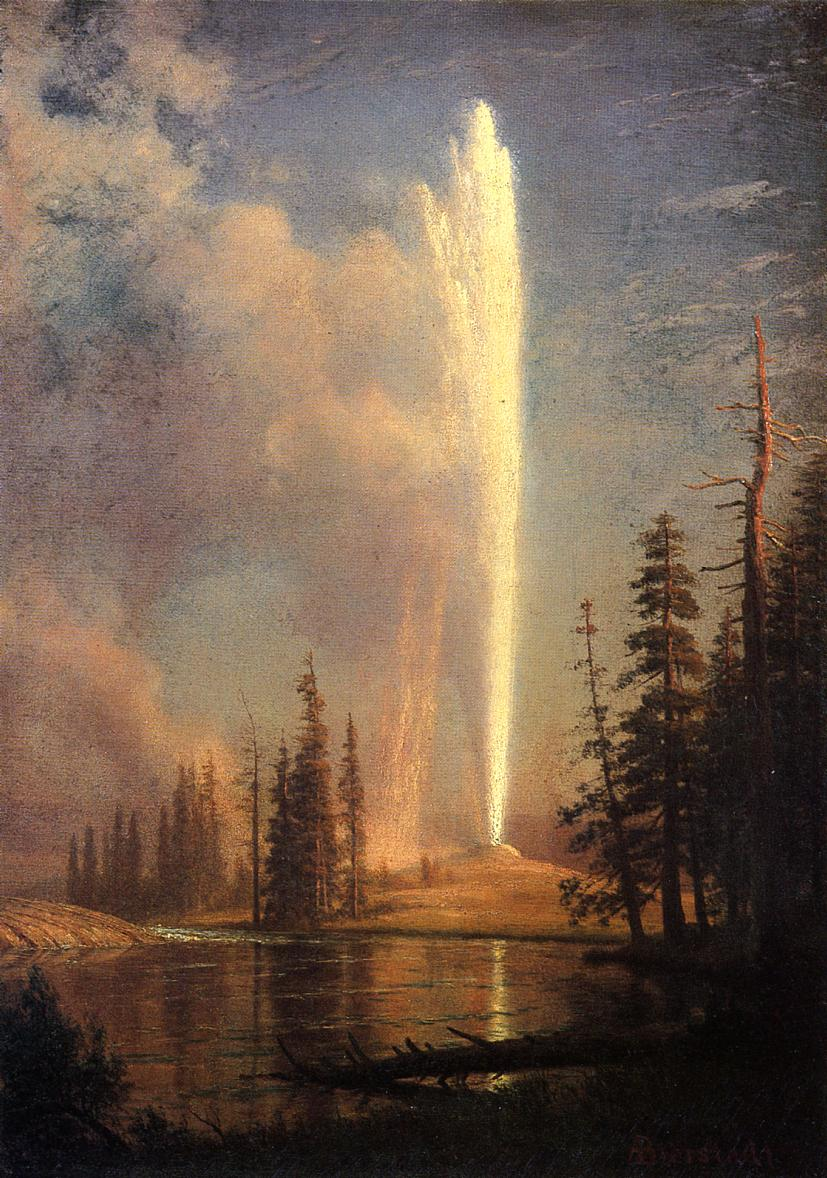
\includegraphics[width=0.8\linewidth]{images/old-faithful} 

}

\caption{Obraz Alberta Bierstadta przedstawiający gejzer Old Faithful około roku 1881. Źródło: \url{https://commons.wikimedia.org/wiki/File:Bierstadt_Albert_Old_Faithful.jpg}}\label{fig:faithful}
\end{figure}

\hypertarget{arkusze-kalkulacyjne}{%
\section{Arkusze kalkulacyjne}\label{arkusze-kalkulacyjne}}

Powszechnym sposobem przechowywania danych tabelarycznych są arkusze kalkulacyjne tworzone w programie Microsoft Excel.
Tego typu dane można wczytać do R używając pakietu \textbf{readxl} \citep{R-readxl}.
Główną funkcją tego pakietu jest \texttt{read\_excel()}, przyjmująca ścieżkę pliku do wczytania.
Dodatkowe argumenty tej funkcji pozwalają, np. na zdefiniowanie arkusza do wczytania (\texttt{sheet}) czy zasięgu komórek (\texttt{range}).

\begin{Shaded}
\begin{Highlighting}[]
\KeywordTok{library}\NormalTok{(readxl)}
\NormalTok{meteo_z_xl =}\StringTok{ }\KeywordTok{read_excel}\NormalTok{(}\StringTok{"pliki/dane_meteo.xlsx"}\NormalTok{)}
\KeywordTok{head}\NormalTok{(meteo_z_xl)}
\CommentTok{#> # A tibble: 6 x 7}
\CommentTok{#>   kod_stacji nazwa_stacji   rok miesiac dzien  tavg}
\CommentTok{#>        <dbl> <chr>        <dbl>   <dbl> <dbl> <dbl>}
\CommentTok{#> 1  352160330 POZNAŃ        2017       1     1   1.4}
\CommentTok{#> 2  352160330 POZNAŃ        2017       1     2   0.1}
\CommentTok{#> 3  352160330 POZNAŃ        2017       1     3   0.5}
\CommentTok{#> 4  352160330 POZNAŃ        2017       1     4   1.5}
\CommentTok{#> 5  352160330 POZNAŃ        2017       1     5  -3.5}
\CommentTok{#> 6  352160330 POZNAŃ        2017       1     6  -8.4}
\CommentTok{#> # ... with 1 more variable: precip <dbl>}
\end{Highlighting}
\end{Shaded}

Do zapisania ramki danych do formatu Excel można użyć funkcji \texttt{write\_xlsx()} z pakietu \textbf{writexl} \citep{R-writexl}\footnote{Po więcej informacji otwórz plik pomocy tej funkcji \texttt{?write\_xlsx()}.}.

\hypertarget{inne-formaty}{%
\section{Inne formaty}\label{inne-formaty}}

Powyżej można było zobaczyć jaki sposób można wczytać dane z różnorodnych plików tekstowych, R, czy arkuszy kalkulacyjnych.
R pozwala jednocześnie na otworzenie wielu innych formatów plików używając dodatkowych pakietów.
Przykładowo, hierarchiczne formaty danych można wczytać używając pakietu \textbf{jsonline} (format \texttt{.json}) \citep{R-jsonlite} czy \textbf{xml2} (format \texttt{.xml}) \citep{R-xml2}, a formaty danych przestrzennych używając pakietu \textbf{sf} (dane wektorowe) \citep{R-sf} czy \textbf{raster} (dane rastrowe) \citep{R-raster}.
Zestawienie zawierające dodatkowe przykłady można znaleźć pod adresem \url{https://github.com/leeper/rio}.

Powszechną sytuacją jest przechowywanie danych w różnego rodzaju bazach danych.
Ma to miejsce, kiedy dane są znacznej wielkości, mają złożone relacje, czy też muszą być jednocześnie dostępne dla wielu osób.
Dostęp do baz danych w R możliwy jest używając pakietu \textbf{DBI} \citep{R-DBI} wraz z dodatkowym pakietem dla konkretnego systemu bazodanowego (np. \textbf{RPostgreSQL} dla baz PostgreSQL \citep{R-RPostgreSQL} czy \textbf{RSQLite} dla baz SQLite \citep{R-RSQLite}). \footnote{Więcej informacji o łączeniu się z bazami danych można znaleść na stronie \url{https://db.rstudio.com/getting-started/connect-to-database}.}

\hypertarget{zadania}{%
\section{Zadania}\label{zadania}}

\begin{enumerate}
\def\labelenumi{\arabic{enumi})}
\item
  Stwórz nowy projekt RStudio o nazwie ``IO''.
  Wszystkie kolejne zadania wykonuj wewnątrz tego projektu.
\item
  Sprawdź jaki jest obecny folder roboczy.
\item
  Stwórz z poziomu R dwa nowe foldery, jeden o nazwie \texttt{"data"} i drugi o nazwie \texttt{"R"}.
\item
  Pobierz plik \texttt{pliki.zip} znajdujący się pod adresem \url{https://github.com/Nowosad/elp/raw/master/}.
  Rozpakuj go do podfolderu \texttt{"data"} i usuń pobrane archiwum z poziomu R.
\item
  Wczytaj dane z pliku \texttt{dane\_meteo.xlsx}.
  Usuń z nowego obiektu pierwszą kolumnę i zapisz go jako plik w binarnym formacie RDS.
\item
  Wczytaj pliki \texttt{dane\_meteo.csv} oraz \texttt{dane\_meteo2.csv} do R.
  Połącz te dwa obiekty łącząc kolumny, a następnie zapisz nowy obiekt do pliku ``.
\item
  Napisz funkcję, która przyjmuje jako argument nazwę folderu, a następnie wczytuje wszystkie pliki o rozszerzeniu \texttt{.csv} znajdujące się w tym folderze i łączy je kolumnami.
\item
  W pliku \texttt{list.txt} znajduje się zaszyfrowana wiadomość.
  Aby ją odczytać należy stworzyć odwrotność jej zawartości, tj. pierwsza linia tekstu w pliku wejściowym ma być ostatnią linią tekstu w przetworzonym obiekcie, a pierwszy znak w danej linii ma stać się ostatnim, itd.
  Napisz funkcję, która odszyfruje tą wiadomość.
\end{enumerate}

\hypertarget{part-narzux119dzia}{%
\part{Narzędzia}\label{part-narzux119dzia}}

\hypertarget{zlozone-funkcje}{%
\chapter{Złożone funkcje}\label{zlozone-funkcje}}

Funkcje są podstawą działania w językach programowania.
Rozdział \ref{funkcje} wprowadził do podstawowych kwestii związanych z funkcjami - jak się używa wbudowanych funkcji oraz jak się tworzy proste nowe funkcje.
Tworzenie bardziej złożonych funkcji czy też zbiorów funkcji wymaga przemyślenia tego nie tylko jak się będą one nazywać, ale też tego jak mogą one zostać użyte przez inne osoby.
W tym rozdziale zostanie podanych kilka porad w jaki sposób budować funkcje przyjazne innym użytkownikom oraz w jaki sposób tworzyć odpowiednie komunikaty błędów, ostrzeżeń czy wiadomości.
Dodatkowo, nastąpi także wprowadzenie do kolejnego paradygmatu programowania - programowania obiektowego.

\hypertarget{api}{%
\section{API}\label{api}}

Interfejs programistyczny aplikacji (ang. \emph{application programming interface}, API) to zbiór sposobów komunikacji pomiędzy różnymi komponentami oprogramowania.
Najszerzej mówiąc API określa w jaki sposób następuje interakcja z kodem i my w tej sekcji skupimy się na tej definicji.
Warto jednak pamiętać, że często osoby, które używają tego skrótu mają tak na prawdę na myśli RESTful API, czyli API które powala na komunikację pomiędzy komputerami poprzez protokół HTTP.

Dobrze zaprojektowane API uławia zarówno rozwijanie oprogramowania, jak i jego używanie.
Podstawowe elementy przemyślanego API w R obejmują nazwy funkcji, ich argumenty, oraz tzw. stabilność typu (ang. \emph{type stability}).

Funkcje wewnątrz pojedynczego pakietu powinny być nazywane konsekwentnie używając tylko jednej konwencji nazywania (sekcja \ref{nazwy-obiektow}).
Sama nazwa powinna w zwięzły sposób przekazywać jakie jest działanie funkcji.
Dodatkową możliwością jest używanie w jednym pakiecie funkcji rozpoczynających się od takiego samego prefiksu.
Przykładowo, większość nazw funkcji w pakiecie \textbf{landscapemetrics} rozpoczyna się od liter \texttt{lsm\_}, np. \texttt{lsm\_l\_ent()} \citep{R-landscapemetrics}.

Podobnie należy stosować tylko jedną konwencję przy nazywaniu argumentów funkcji, a nazwy argumentów powinny być informacyjne, ale jednocześnie zwięzłe.
W przypadku, gdy taki sam rodzaj danych wejściowych jest oczekiwany w różnych funkcjach, koniecznie jest aby zawsze ten argument był tak samo nazwany.
Podobnie należy zadbać o spójną kolejność podobnych argumentów w funkcjach jednego pakietu.

Stabilność typu oznacza, że używając jednej klasy danych wejściowych funkcja zawsze zwróci obiekt jednej klasy.
Poniższy przykład użycia funkcji \texttt{grep()} pokazuje, że nie ma ona stabilności typu.
Zalecane jest unikanie tworzenia funkcji bez stabilności typu.

\begin{Shaded}
\begin{Highlighting}[]
\NormalTok{tekst =}\StringTok{ }\KeywordTok{c}\NormalTok{(}\StringTok{"kołdra"}\NormalTok{, }\StringTok{"kordła"}\NormalTok{, }\StringTok{"pościel"}\NormalTok{)}
\KeywordTok{grep}\NormalTok{(}\StringTok{"^[k]."}\NormalTok{, }\DataTypeTok{x =}\NormalTok{ tekst)}
\CommentTok{#> [1] 1 2}
\KeywordTok{grep}\NormalTok{(}\StringTok{"^[k]."}\NormalTok{, }\DataTypeTok{x =}\NormalTok{ tekst, }\DataTypeTok{value =} \OtherTok{TRUE}\NormalTok{)}
\CommentTok{#> [1] "kołdra" "kordła"}
\end{Highlighting}
\end{Shaded}

Dodatkowym elementem API może być określenie domyślnych parametrów funkcji.
Poniższa funkcja, \texttt{potegowanie()} ma na celu podnoszenie wartości wejściowego wektora (\texttt{x}) do wybranej potęgi (\texttt{w}).
Domyślamy się jednak, że większość użytkowników jest zainteresowana używaniem tej funkcji do podnoszenia wartości do drugiej potęgi i dlatego też ustalamy, że domyślnie argument \texttt{w} przyjmuje wartość 2.

\begin{Shaded}
\begin{Highlighting}[]
\NormalTok{potegowanie =}\StringTok{ }\ControlFlowTok{function}\NormalTok{(x, }\DataTypeTok{w =} \DecValTok{2}\NormalTok{)\{}
\NormalTok{  x }\OperatorTok{^}\StringTok{ }\NormalTok{w}
\NormalTok{\}}
\end{Highlighting}
\end{Shaded}

W tej sytuacji, gdy użytkownik poda tylko jeden argument do funkcji \texttt{potegowanie()} to podany wektor zostanie podniesiony do kwadratu.

\begin{Shaded}
\begin{Highlighting}[]
\KeywordTok{potegowanie}\NormalTok{(}\DecValTok{2}\NormalTok{)}
\CommentTok{#> [1] 4}
\end{Highlighting}
\end{Shaded}

Będzie to identyczne z działaniem funkcji, gdy użytkownik ręcznie zdefiniuje drugi argument jako dwa (\texttt{w\ =\ 2}).

\begin{Shaded}
\begin{Highlighting}[]
\KeywordTok{potegowanie}\NormalTok{(}\DecValTok{2}\NormalTok{, }\DataTypeTok{w =} \DecValTok{2}\NormalTok{)}
\CommentTok{#> [1] 4}
\end{Highlighting}
\end{Shaded}

W sytuacji, gdy użytkownika interesuje inna wartość \texttt{w} niż domyślna, może on ją zmodyfikować i otrzyma odpowiedni wynik.

\begin{Shaded}
\begin{Highlighting}[]
\KeywordTok{potegowanie}\NormalTok{(}\DecValTok{2}\NormalTok{, }\DataTypeTok{w =} \DecValTok{3}\NormalTok{)}
\CommentTok{#> [1] 8}
\end{Highlighting}
\end{Shaded}

\hypertarget{obsluga-komunikatow}{%
\section{Obsługa komunikatów}\label{obsluga-komunikatow}}

W sekcji \ref{komunikaty} omówiliśmy trzy podstawowe rodzaje komunikatów: błędy, ostrzeżenia i wiadomości.
Teraz zobaczmy jak te zaimplementować we własnych funkcjach i kiedy powinny być one użyte.

Obsługa błędów w funkcjach ma na celu ochronę użytkownika przed nieodpowiednim zachowaniem funkcji.
Komunikat błędu powinien ułatwiać użytkownikowi zrozumienie problemu oraz jego rozwiązanie.
Zazwyczaj komunikat błędu przyjmuje jedną z trzech form: (1) określenie problemu, np. \texttt{Argument\ \textquotesingle{}x\textquotesingle{}\ musi\ być\ zmienną\ numeryczną,\ a\ nie\ znakową.}, (2) lokalizacja błędu, np. \texttt{Kolumna\ \textquotesingle{}abc\textquotesingle{}\ nie\ istnieje\ w\ obiekcie\ \textquotesingle{}y\textquotesingle{}.}, (3) porada, np. \texttt{Did\ you\ mean\ \textquotesingle{}Species\ ==\ "setosa"\textquotesingle{}?}.
Oczywiście te wymienione formy można łączyć.

Ważne jest też, aby funkcja kończyła swoje działanie jak najszybciej po napotkaniu, np. błędnych wartości wejściowych.
Żadnej użytkownik nie chce czekać na zakończenie wykonywania długiej funkcji zanim dostanie komunikat błędu.
Więcej informacji o strukturze komunikatów błędów można znaleźć na \url{https://style.tidyverse.org/error-messages.html}.

Do zatrzymania działania funkcji i wyświetlenia komunikatu błędu służy \texttt{stop()}.

\begin{Shaded}
\begin{Highlighting}[]
\KeywordTok{stop}\NormalTok{(}\StringTok{"To jest komunikat błędu."}\NormalTok{)}
\CommentTok{#> Error in eval(expr, envir, enclos): To jest komunikat błędu.}
\end{Highlighting}
\end{Shaded}

Ostrzeżenia mogą być używane w wielu różnorodnych sytuacjach, np. kiedy chcesz poinformować użytkowników o tym, że dana funkcja zostanie wygaszona lub przeniesiona do innego pakietu.
Komunikaty ostrzeżenia tworzyć się używając funkcji \texttt{warning()}.

\begin{Shaded}
\begin{Highlighting}[]
\KeywordTok{warning}\NormalTok{(}\StringTok{"To jest komunikat ostrzeżenia."}\NormalTok{)}
\CommentTok{#> Warning: To jest komunikat ostrzeżenia.}
\end{Highlighting}
\end{Shaded}

Wiadomości mają na celu poinformowanie użytkownika na temat działania pakietu lub funkcji.
Są one wykorzystywane podczas wczytywania niektórych pakietów.
Innym przykładem jest informowanie na temat działania funkcji w tle - pobierania danych, zapisywania do pliku, czy przeliczania cząstkowych parametrów.
Do wyświetlenia wiadomości służy funkcja \texttt{message()}.

\begin{Shaded}
\begin{Highlighting}[]
\KeywordTok{message}\NormalTok{(}\StringTok{"To jest komunikat wiadomości."}\NormalTok{)}
\CommentTok{#> To jest komunikat wiadomości.}
\end{Highlighting}
\end{Shaded}

\begin{rmdinfo}
Działanie funkcji \texttt{message()} jest zbliżone do funkcji \texttt{cat()} czy \texttt{print()}.
Różni je jednak cel w jakim są użyte.
Rolą funkcji \texttt{message()} jest przekazanie informacji od twórcy do użytkownika, natomiast celem funkcji tj. \texttt{cat()} jest zapytanie użytkownika w pewnej kwestii.
\end{rmdinfo}

Przykład użycia trzech podstawowych rodzajów komunikatów można zobaczyć w poniższej funkcji \texttt{minus\_1()}.
Ta funkcja przyjmuje wartość numeryczną, od której odejmuje jeden, a na końcu zwraca wartość bezwzględną (\texttt{abs(x\ -\ 1)}).

\begin{Shaded}
\begin{Highlighting}[]
\NormalTok{minus_}\DecValTok{1}\NormalTok{ =}\StringTok{ }\ControlFlowTok{function}\NormalTok{(x)\{}
  \ControlFlowTok{if}\NormalTok{(}\KeywordTok{is.character}\NormalTok{(x))\{}
    \KeywordTok{stop}\NormalTok{(}\StringTok{"Argument `x` musi być zmienną numeryczną, a nie znakową."}\NormalTok{)}
\NormalTok{  \} }\ControlFlowTok{else} \ControlFlowTok{if}\NormalTok{(}\KeywordTok{is.logical}\NormalTok{(x))\{}
    \KeywordTok{warning}\NormalTok{(}\KeywordTok{paste}\NormalTok{(}\StringTok{"Argument `x` jest zmienną logiczną."}\NormalTok{,}
                  \StringTok{"Czy nie chcesz użyć zmiennej numerycznej?"}\NormalTok{))}
\NormalTok{  \} }\ControlFlowTok{else}\NormalTok{ \{}
    \KeywordTok{message}\NormalTok{(}\StringTok{"Wow. Argument `x` jest oczekiwaną zmienną numeryczną."}\NormalTok{)}
\NormalTok{  \}}
  \KeywordTok{abs}\NormalTok{(x }\OperatorTok{-}\StringTok{ }\DecValTok{1}\NormalTok{)}
\NormalTok{\}}
\end{Highlighting}
\end{Shaded}

W przypadku, gdy użytkownik wprowadzi jako wejście wektor tekstowy (\texttt{if(is.character(x))}) to działanie funkcji zostanie przerwane i pojawi się odpowiedni komunikat błędu.

\begin{Shaded}
\begin{Highlighting}[]
\KeywordTok{minus_1}\NormalTok{(}\StringTok{"kot"}\NormalTok{)}
\CommentTok{#> Error in minus_1("kot"): Argument `x` musi być zmienną numeryczną, a nie znakową.}
\end{Highlighting}
\end{Shaded}

Jeżeli jako argument \texttt{x} zostanie podany wektor logiczny (\texttt{else\ if(is.logical(x))}) to pojawi się komunikat ostrzeżenia, ale dalsze obliczanie zostanie wykonane.
W tym przypadku wartość \texttt{TRUE} zostanie najpierw zamieniona na jeden a \texttt{FALSE} na zero, następnie od tych wartości zostanie odjęte jeden, a na końcu zostaną one zamienione na wartości bezwzględne.

\begin{Shaded}
\begin{Highlighting}[]
\KeywordTok{minus_1}\NormalTok{(}\KeywordTok{c}\NormalTok{(}\OtherTok{TRUE}\NormalTok{, }\OtherTok{FALSE}\NormalTok{))}
\CommentTok{#> Warning in minus_1(c(TRUE, FALSE)): Argument `x`}
\CommentTok{#> jest zmienną logiczną. Czy nie chcesz użyć zmiennej}
\CommentTok{#> numerycznej?}
\CommentTok{#> [1] 0 1}
\end{Highlighting}
\end{Shaded}

Po wprowadzeniu wartości numerycznych do funkcji \texttt{minus\_1()} pojawi się tekst wiadomości, po którym nastąpi wyliczenie kodu \texttt{abs(x\ -\ 1)}.

\begin{Shaded}
\begin{Highlighting}[]
\KeywordTok{minus_1}\NormalTok{(}\KeywordTok{c}\NormalTok{(}\DecValTok{1}\NormalTok{, }\DecValTok{0}\NormalTok{, }\DecValTok{6}\NormalTok{, }\DecValTok{-6}\NormalTok{))}
\CommentTok{#> Wow. Argument `x` jest oczekiwaną zmienną numeryczną.}
\CommentTok{#> [1] 0 1 5 7}
\end{Highlighting}
\end{Shaded}

Złożone funkcje opierają się o inne istniejące funkcje.
W powyższym przykładzie, \texttt{minus\_1()} używał, między innymi funkcji \texttt{-} do odejmowania czy \texttt{abs} do wyliczania wartości bezwzględnej.
Czasami spodziewamy się, że wartość wprowadzona przez użytkownika może spowodować wystąpienie wewnętrznego błędu i jednocześnie wiemy jak to naprawić.
W takich sytuacjach przydaje się funkcja \texttt{tryCatch()}.

\begin{rmdinfo}
R pozwala na ignorowanie wystąpienia błędu używając funkcji \texttt{try()}, ignorowanie ostrzeżeń z \texttt{suppressWarnings()} oraz wiadomości z \texttt{suppressMessages()}.
\end{rmdinfo}

\texttt{tryCatch()} stara się uruchomić jakiś wskazany kod, a w przypadku pojawienia się błędu wykonuje alternatywne obliczenia.
Można to zobaczyć na poniższym przykładzie, gdzie najpierw sprawdzona zostałaby linia \texttt{kod\ do\ uruchomienia} i dopiero gdyby ona skutkowała błędem zostałaby uruchomiona linia \texttt{wykonaj\ kod\ w\ przypadku\ wystąpienia\ błędu}.

\begin{Shaded}
\begin{Highlighting}[]
\KeywordTok{tryCatch}\NormalTok{(}
  \DataTypeTok{error =} \ControlFlowTok{function}\NormalTok{(e) \{}
\NormalTok{    wykonaj kod w przypadku wystąpienia błędu}
\NormalTok{  \},}
\NormalTok{  kod do uruchomienia }
\NormalTok{)}
\end{Highlighting}
\end{Shaded}

Działanie \texttt{tryCatch} w praktyce jest pokazane w funkcji \texttt{log\_safe()}.
Stara się ona wyliczyć logarytm naturalny (\texttt{log()}) z wartości argumentu \texttt{x}, a w przypadku gdyby napotkała błąd zwróci ona wartość \texttt{NA}.

\begin{Shaded}
\begin{Highlighting}[]
\NormalTok{log_safe =}\StringTok{ }\ControlFlowTok{function}\NormalTok{(x)\{}
  \KeywordTok{tryCatch}\NormalTok{(}
  \DataTypeTok{error =} \ControlFlowTok{function}\NormalTok{(e) \{}
    \OtherTok{NA}
\NormalTok{  \},}
  \KeywordTok{log}\NormalTok{(x)}
\NormalTok{  )}
\NormalTok{\}}
\end{Highlighting}
\end{Shaded}

Sprawdźmy jej zachowanie na dwóch przykładach.
W pierwszym oryginalna funkcja \texttt{log()} jak i nowa \texttt{log\_safe()} otrzymają poprawne dane wejściowe - wektor numeryczny.

\begin{Shaded}
\begin{Highlighting}[]
\KeywordTok{log}\NormalTok{(}\DecValTok{10}\NormalTok{)}
\CommentTok{#> [1] 2.3}
\KeywordTok{log_safe}\NormalTok{(}\DecValTok{10}\NormalTok{)}
\CommentTok{#> [1] 2.3}
\end{Highlighting}
\end{Shaded}

W tym przypadku obie zwracają dokładnie taki sam wynik.
Jeżeli jednak jako dane wejściowe wprowadzimy wektor znakowy to oryginalna funkcja zwróci błąd, a nasza funkcja jedynie wartość \texttt{NA}.

\begin{Shaded}
\begin{Highlighting}[]
\KeywordTok{log}\NormalTok{(}\StringTok{"abecadło"}\NormalTok{)}
\CommentTok{#> Error in log("abecadło"): non-numeric argument to mathematical function}
\end{Highlighting}
\end{Shaded}

\begin{Shaded}
\begin{Highlighting}[]
\KeywordTok{log_safe}\NormalTok{(}\StringTok{"abecadło"}\NormalTok{)}
\CommentTok{#> [1] NA}
\end{Highlighting}
\end{Shaded}

\begin{rmdinfo}
Dodatkowo istnieje funkcja \texttt{withCallingHandlers()}, która jest używana w przypadku działania na ostrzeżeniach.
\end{rmdinfo}

\hypertarget{oop}{%
\section{Programowanie obiektowe}\label{oop}}

Programowanie obiektowe (ang. \emph{object-oriented programming}, OOP) to jeden z najpopularniejszych paradygmatów programowania (sekcja \ref{jezyki-programowania}).
Polega on na definiowaniu obiektów danej klasy posiadających pewną określoną strukturę oraz zachowania.

R pozwala również na stosowanie paradygmatu obiektowego.
Co więcej, w tym języku istnieje kilka różnych systemów programowania obiektowego, między innymi S3, S4 czy R6.
Każdy z nich charakteryzuje inny sposób tworzenia obiektów czy ich zachowań.
W tym rozdziale skupimy się na najczęściej używanego systemu S3.

Dwa najważniejsze elementy tego systemu to klasy i metody.
Klasa obejmuje obiekty o podobnej strukturze, które posiadają specjalną informację o nazwie klasy.
Metoda natomiast to sposób zachowania funkcji w przypadku napotkania obiektu danej klasy.
Przykład metody był pokazany w sekcji \ref{inne-klasy}, gdzie funkcja \texttt{mean()} zachowywała się różnie w zależności od klasy danych wejściowych.

\hypertarget{klasy}{%
\subsection{Klasy}\label{klasy}}

Poniżej stworzono nową macierz \texttt{x}, która składa się z dwóch kolumn i dwóch wierszy oraz wartości 0, 0, 2 i 3.
Ma ona na celu reprezentowanie figury geometrycznej - prostokąta.
W najprostszej postaci prostokąt można opisać używając czterech współrzędnych - najmniejszej wartości położenia na osi x (np., \texttt{0}), najmniejszej wartości położenia na osi y (np., \texttt{0}), największej wartości położenia na osi x (np., \texttt{2}), oraz największej wartości położenia na osi y (np., \texttt{3}).

\begin{Shaded}
\begin{Highlighting}[]
\NormalTok{x =}\StringTok{ }\KeywordTok{matrix}\NormalTok{(}\KeywordTok{c}\NormalTok{(}\DecValTok{0}\NormalTok{, }\DecValTok{0}\NormalTok{, }\DecValTok{2}\NormalTok{, }\DecValTok{3}\NormalTok{), }\DataTypeTok{ncol =} \DecValTok{2}\NormalTok{)}
\NormalTok{x}
\CommentTok{#>      [,1] [,2]}
\CommentTok{#> [1,]    0    2}
\CommentTok{#> [2,]    0    3}
\end{Highlighting}
\end{Shaded}

Do sprawdzenia klasy obiektu w systemie S3 służy funkcja \texttt{class()}.

\begin{Shaded}
\begin{Highlighting}[]
\KeywordTok{class}\NormalTok{(x)}
\CommentTok{#> [1] "matrix" "array"}
\end{Highlighting}
\end{Shaded}

W efekcie upewniamy się, że klasa naszego obiektu \texttt{x} to matrix, array.
System S3 pozwala na prostą zmianę lub dodanie nazwy klasy używając funkcji \texttt{structure()}.

\begin{Shaded}
\begin{Highlighting}[]
\NormalTok{y =}\StringTok{ }\KeywordTok{structure}\NormalTok{(x, }\DataTypeTok{class =} \StringTok{"prostokat"}\NormalTok{)}
\end{Highlighting}
\end{Shaded}

Wynikiem działania tej funkcji z argumentem \texttt{class\ =\ "prostokat"} jest nowy obiekt \texttt{y}.
W momencie, gdy sprawdzimy jego klasę, okaże się że nie jest to już matrix, array ale prostokat.

\begin{Shaded}
\begin{Highlighting}[]
\KeywordTok{class}\NormalTok{(y)}
\CommentTok{#> [1] "prostokat"}
\end{Highlighting}
\end{Shaded}

\hypertarget{metody}{%
\subsection{Metody}\label{metody}}

Posiadamy teraz nową klasę, \texttt{prostokat}, ale nie posiadamy do niej żadnych metod.
Metoda w systemie S3 to funkcja, która działa w różny sposób w zależności od klasy danych wejściowych.
Możliwe jest zarówno dodanie nowej metody do istniejącej funkcji, jak i stworzenie nowej funkcji.

W tym wypadku interesuje nas możliwość policzenia powierzchni.
Możemy do tego celu stworzyć nową funkcję w systemie S3 o nazwie \texttt{powierzchnia}.
Pierwszym krokiem musi być określenie, że nasza funkcja ma być oparta o system S3 używając poniższej formy.

\begin{Shaded}
\begin{Highlighting}[]
\NormalTok{powierzchnia =}\StringTok{ }\ControlFlowTok{function}\NormalTok{(x) \{}
  \KeywordTok{UseMethod}\NormalTok{(}\StringTok{"powierzchnia"}\NormalTok{)}
\NormalTok{\}}
\end{Highlighting}
\end{Shaded}

Drugim krokiem jest zdefiniowanie funkcji do wyliczania powierzchni prostokąta.
Określa ona najpierw długości boków a i b, a następnie wymnaża je w celu wyliczenia powierzchni.

\begin{Shaded}
\begin{Highlighting}[]
\NormalTok{powierzchnia.prostokat =}\StringTok{ }\ControlFlowTok{function}\NormalTok{(x)\{}
\NormalTok{  a =}\StringTok{ }\NormalTok{x[}\DecValTok{1}\NormalTok{, }\DecValTok{2}\NormalTok{] }\OperatorTok{-}\StringTok{ }\NormalTok{x[}\DecValTok{1}\NormalTok{, }\DecValTok{1}\NormalTok{] }\CommentTok{#wyliczenie długości boku a}
\NormalTok{  b =}\StringTok{ }\NormalTok{x[}\DecValTok{2}\NormalTok{, }\DecValTok{2}\NormalTok{] }\OperatorTok{-}\StringTok{ }\NormalTok{x[}\DecValTok{2}\NormalTok{, }\DecValTok{1}\NormalTok{] }\CommentTok{#wyliczenie długości boku b}
\NormalTok{  a }\OperatorTok{*}\StringTok{ }\NormalTok{b                 }\CommentTok{#wyliczenie powierzchni prostokąta}
\NormalTok{\}}
\end{Highlighting}
\end{Shaded}

Nazwa powyższej funkcji wygląda jakby składała się z dwóch słów oddzielonych kropką - \texttt{powierzchnia.prostokat}.
W rzeczywistości jednak nazwa funkcji to tylko \texttt{powierzchnia}, a kropka sugeruje że kolejny po niej wyraz to klasa obiektu jaki przyjmie funkcja.
Jest to, innymi słowy, definicja metody.
Nowa funkcja \texttt{powierzchnia} zadziała w powyższy sposób tylko w wypadku otrzymania jako dane wejściowe obiektu klasy \texttt{prostokat}.

Sprawdźmy to na dwóch przykładach - obiektu \texttt{y} (klasa \texttt{prostokat}) i \texttt{x} (klasa \texttt{matrix}).

\begin{Shaded}
\begin{Highlighting}[]
\NormalTok{y}
\CommentTok{#>      [,1] [,2]}
\CommentTok{#> [1,]    0    2}
\CommentTok{#> [2,]    0    3}
\CommentTok{#> attr(,"class")}
\CommentTok{#> [1] "prostokat"}
\KeywordTok{powierzchnia}\NormalTok{(y)}
\CommentTok{#> [1] 6}
\end{Highlighting}
\end{Shaded}

W przypadku, gdy nasz obiekt wejściowy jest klasy \texttt{prostokat} to funkcja jest wykonywana zgodnie z metodą \texttt{powierzchnia.prostokat()},

\begin{Shaded}
\begin{Highlighting}[]
\NormalTok{x}
\CommentTok{#>      [,1] [,2]}
\CommentTok{#> [1,]    0    2}
\CommentTok{#> [2,]    0    3}
\KeywordTok{powierzchnia}\NormalTok{(x)}
\CommentTok{#> Error in UseMethod("powierzchnia"): no applicable method for 'powierzchnia' applied to an object of class "c('matrix', 'array', 'double', 'numeric')"}
\end{Highlighting}
\end{Shaded}

Natomiast, gdy obiekt wejściowy będzie innej klasy to pojawi się komunikat błędu sugerujący, że nie istnieje metoda dla tej klasy pozwalająca na otrzymanie wyniku.

Dodatkowo, oprócz tworzenia metod dla każdej klasy oddzielnie możliwe jest stworzenie metody domyślnej poprzez \texttt{nazwafunkcji.default}.
W przypadku, gdy dla obiektu wejściowego nie istnieje metoda to wówczas wykonywana jest metoda domyślna (\texttt{default}).
Poniżej dodano metodę domyślną - w przypadku, gdy dla wejściowego obiektu nie ma metody to pojawi się poniższy komunikat błędu.

\begin{Shaded}
\begin{Highlighting}[]
\NormalTok{powierzchnia.default =}\StringTok{ }\ControlFlowTok{function}\NormalTok{(x) \{}
  \KeywordTok{stop}\NormalTok{(}\StringTok{"Funkcja `powierzchnia` ma wsparcie tylko dla obiektów o klasie `prostokąt`"}\NormalTok{)}
\NormalTok{\}}
\end{Highlighting}
\end{Shaded}

Sprawdźmy działanie domyślnej metody podając macierz jako obiekt wejściowy.

\begin{Shaded}
\begin{Highlighting}[]
\NormalTok{x}
\CommentTok{#>      [,1] [,2]}
\CommentTok{#> [1,]    0    2}
\CommentTok{#> [2,]    0    3}
\KeywordTok{powierzchnia}\NormalTok{(x)}
\CommentTok{#> Error in powierzchnia.default(x): Funkcja `powierzchnia` ma wsparcie tylko dla obiektów o klasie `prostokąt`}
\end{Highlighting}
\end{Shaded}

\hypertarget{konstruktory}{%
\subsection{Konstruktory}\label{konstruktory}}

Trudno oczekiwać od użytkownika, że bez żadnych pomyłek stworzy obiekt klasy, który wymyśliliśmy, a następnie użyje funkcji \texttt{structure()}, aby dodać odpowiednią nazwę klasy.
Dlatego też ważnym elementem jest stworzenie konstruktora - funkcji, której celem jest zbudowanie poprawnego obiektu naszej klasy, a w przypadku podania złych argumentów wejściowych poinformowanie użytkownika co jest nie tak.

Poniżej znajduje się konstruktor o nazwie \texttt{nowy\_prostokąt()}. Przyjmuje on wartości czterech współrzędnych, a następnie wykonuje szereg sprawdzeń ich poprawności:

\begin{itemize}
\tightlist
\item
  Czy wszystkie argumenty są typu numerycznego?
\item
  Czy każdy argument ma tylko jeden element?
\item
  Czy minimalna wartość współrzędnej x jest mniejsza od maksymalnej?
\item
  Czy minimalna wartość współrzędnej y jest mniejsza od maksymalnej?
\end{itemize}

Po tych sprawdzeniach następuje zbudowanie nowej macierzy oraz dodanie nazwy klasy.

\begin{Shaded}
\begin{Highlighting}[]
\NormalTok{nowy_prostokat =}\StringTok{ }\ControlFlowTok{function}\NormalTok{(xmin, ymin, xmax, ymax)\{}
\NormalTok{  vals =}\StringTok{ }\KeywordTok{c}\NormalTok{(xmin, ymin, xmax, ymax)}
  \ControlFlowTok{if}\NormalTok{ (}\OperatorTok{!}\NormalTok{(}\KeywordTok{is.numeric}\NormalTok{(vals)))\{}
    \KeywordTok{stop}\NormalTok{(}\StringTok{"Wszystkie argumenty muszą być typu numerycznego"}\NormalTok{)}
\NormalTok{  \}}
  \ControlFlowTok{if}\NormalTok{ (}\OperatorTok{!}\KeywordTok{all}\NormalTok{(}\KeywordTok{c}\NormalTok{(}\KeywordTok{length}\NormalTok{(xmin), }\KeywordTok{length}\NormalTok{(ymin), }\KeywordTok{length}\NormalTok{(xmax), }\KeywordTok{length}\NormalTok{(ymax)) }\OperatorTok{==}\StringTok{ }\DecValTok{1}\NormalTok{))\{}
    \KeywordTok{stop}\NormalTok{(}\StringTok{"Każdy z argumentów może przyjmować tylko jedną wartość"}\NormalTok{)}
\NormalTok{  \}}
\NormalTok{  x_range =}\StringTok{ }\NormalTok{vals[}\DecValTok{3}\NormalTok{] }\OperatorTok{-}\StringTok{ }\NormalTok{vals[}\DecValTok{1}\NormalTok{]}
  \ControlFlowTok{if}\NormalTok{ (x_range }\OperatorTok{<=}\StringTok{ }\DecValTok{0}\NormalTok{)\{}
    \KeywordTok{stop}\NormalTok{(}\StringTok{"`xmax` musi przyjmować wartość większą niż `xmin`"}\NormalTok{)}
\NormalTok{  \}}
\NormalTok{  y_range =}\StringTok{ }\NormalTok{vals[}\DecValTok{4}\NormalTok{] }\OperatorTok{-}\StringTok{ }\NormalTok{vals[}\DecValTok{2}\NormalTok{]}
  \ControlFlowTok{if}\NormalTok{ (y_range }\OperatorTok{<=}\StringTok{ }\DecValTok{0}\NormalTok{) \{}
    \KeywordTok{stop}\NormalTok{(}\StringTok{"`ymax` musi przyjmować wartość większą niż `ymin`"}\NormalTok{)}
\NormalTok{  \}}
\NormalTok{  x =}\StringTok{ }\KeywordTok{matrix}\NormalTok{(vals, }\DataTypeTok{ncol =} \DecValTok{2}\NormalTok{)}
  \KeywordTok{structure}\NormalTok{(x, }\DataTypeTok{class =} \StringTok{"prostokat"}\NormalTok{)}
\NormalTok{\}}
\end{Highlighting}
\end{Shaded}

Sprawdźmy działanie tego konstruktora na dwóch przypadkach.
W pierwszym podajmy poprawne, sprawdzone wcześniej wartości.

\begin{Shaded}
\begin{Highlighting}[]
\NormalTok{nowy_p =}\StringTok{ }\KeywordTok{nowy_prostokat}\NormalTok{(}\DecValTok{0}\NormalTok{, }\DecValTok{0}\NormalTok{, }\DecValTok{2}\NormalTok{, }\DecValTok{3}\NormalTok{)}
\NormalTok{nowy_p}
\CommentTok{#>      [,1] [,2]}
\CommentTok{#> [1,]    0    2}
\CommentTok{#> [2,]    0    3}
\CommentTok{#> attr(,"class")}
\CommentTok{#> [1] "prostokat"}
\end{Highlighting}
\end{Shaded}

Konstruktor \texttt{nowy\_prostokat()} działa bez problemu, zwracając nowy obiekt \texttt{nowy\_p} o klasie \texttt{prostokat}.
Warto od razu zobaczyć, czy ten obiekt zadziała poprawnie w funkcji \texttt{powierzchnia()}.

\begin{Shaded}
\begin{Highlighting}[]
\KeywordTok{powierzchnia}\NormalTok{(nowy_p)}
\CommentTok{#> [1] 6}
\end{Highlighting}
\end{Shaded}

W przypadku, gdy do konstruktora zostaną podane niepoprawne wartości wejściowe pojawi się odpowiedni komunikat błędu.

\begin{Shaded}
\begin{Highlighting}[]
\NormalTok{nowy_p2 =}\StringTok{ }\KeywordTok{nowy_prostokat}\NormalTok{(}\DecValTok{7}\NormalTok{, }\DecValTok{0}\NormalTok{, }\DecValTok{6}\NormalTok{, }\DecValTok{0}\NormalTok{)}
\CommentTok{#> Error in nowy_prostokat(7, 0, 6, 0): `xmax` musi przyjmować wartość większą niż `xmin`}
\end{Highlighting}
\end{Shaded}

\hypertarget{zadania}{%
\section{Zadania}\label{zadania}}

\begin{enumerate}
\def\labelenumi{\arabic{enumi})}
\item
  Bez pisania kodu, zaprojektuj API zbioru funkcji R pozwalających na tworzenie podstawowych obiektów reprezentujących podstawowe figury (np. kwadrat, prostokąt, koło, trójkąt, itd.) oraz wyliczania na ich podstawie podstawowych miar (np. obwód, pole powierzchni, itd.).
  Nowe API powinno obejmować nazwy funkcji, nazwy ich argumentów, istnienie lub brak domyślnych wartości argumentów, klasy obiektów wejściowych i wyjściowych z tych funkcji, itd.
\item
  Stwórz nową klasę obiektów w R reprezentujących trójkąty.
  Nazwij tą nową klasę \texttt{"trojkat"}.
  W jaki sposób trójkąty będą reprezentowane w tej nowej klasie?
  (Podpowiedź: w zależności od podjętej decyzji nowa klasa może być oparta o wektory, macierze lub ramki danych.)
\item
  Dodaj konstruktor pozwalający innym użytkownikom na tworzenie obiektów klasy \texttt{"trojkat"}.
  Zastanów się jakie powinny być wartości argumentów wejściowych i napisz wewnątrz konstruktora odpowiednie sprawdzenia używając komunikatów błędów, ostrzeżeń czy też wiadomości.
\item
  Stwórz metodę pozwalającą na wyliczanie powierzchni trójkąta.
\item
  Stwórz metodę pozwalającą na określanie współrzędnych centroidu trójkąta.
\end{enumerate}

\hypertarget{analiza-kodu}{%
\chapter{Analiza kodu}\label{analiza-kodu}}

Programując naszym celem jest tworzenie funkcji, które są zarówno poprawne oraz wydajne (zwracają wynik szybko).
W tym rozdziale przedstawione będą testy jednostkowe, które sprawdzają czy funkcje zwracają oczekiwany wynik oraz metody sprawdzające wydajność funkcji, takie jak, profiling i benchmarking.

\hypertarget{testy-jednostkowe}{%
\section{Testy jednostkowe}\label{testy-jednostkowe}}

Testy jednostkowe (ang. \emph{unit tests}) to sposób sprawdzania czy stworzona przez nas funkcja działa w sposób jaki oczekujemy.
Tworzenie takich testów wymusza także myślenie na temat odpowiedniego działania funkcji i jej API.
Testy jednostkowe są najczęściej stosowane w przypadku budowania pakietów (sekcja \ref{wbudowane-testy}), gdzie możliwe jest automatyczne sprawdzenie wielu testów na raz.
Przykładowo, napisaliśmy nową funkcję, która wykonuje złożone operacje i, po wielu sprawdzeniach, wiemy, że daje poprawne wyniki.
Po kilku miesiącach wpadliśmy na pomysł jak zwiększyć wydajność naszej funkcji.
W tym momencie wystarczy już tylko stworzyć nową implementację i użyć wcześniej zbudowanych testów.
Dadzą one informację, czy efekt działania jest taki jaki oczekujemy, a w przeciwnym razie wskażą gdzie pojawił się~błąd.
Istnieje też dodatkowa reguła - jeżeli znajdziesz błąd w kodzie od razu napisz test jednostkowy.

Zobaczmy jak działają testy jednostkowe na przykładzie funkcji \texttt{nowy\_prostokat()} oraz \texttt{powierzchnia()} stworzonych w sekcji \ref{oop}.

\begin{Shaded}
\begin{Highlighting}[]
\NormalTok{nowy_prostokat =}\StringTok{ }\ControlFlowTok{function}\NormalTok{(xmin, ymin, xmax, ymax)\{}
  \ControlFlowTok{if}\NormalTok{ (}\OperatorTok{!}\KeywordTok{all}\NormalTok{(}\KeywordTok{c}\NormalTok{(}\KeywordTok{length}\NormalTok{(xmin), }\KeywordTok{length}\NormalTok{(ymin), }\KeywordTok{length}\NormalTok{(xmax), }\KeywordTok{length}\NormalTok{(ymax)) }\OperatorTok{==}\StringTok{ }\DecValTok{1}\NormalTok{))\{}
    \KeywordTok{stop}\NormalTok{(}\StringTok{"Każdy z argumentów może przyjmować tylko jedną wartość"}\NormalTok{)}
\NormalTok{  \}}
\NormalTok{  vals =}\StringTok{ }\KeywordTok{c}\NormalTok{(xmin, ymin, xmax, ymax)}
  \ControlFlowTok{if}\NormalTok{ (}\OperatorTok{!}\NormalTok{(}\KeywordTok{is.numeric}\NormalTok{(vals)))\{}
    \KeywordTok{stop}\NormalTok{(}\StringTok{"Wszystkie argumenty muszą być typu numerycznego"}\NormalTok{)}
\NormalTok{  \}}
\NormalTok{  x =}\StringTok{ }\KeywordTok{matrix}\NormalTok{(vals, }\DataTypeTok{ncol =} \DecValTok{2}\NormalTok{)}
  \KeywordTok{structure}\NormalTok{(x, }\DataTypeTok{class =} \StringTok{"prostokat"}\NormalTok{)}
\NormalTok{\}}
\NormalTok{powierzchnia =}\StringTok{ }\ControlFlowTok{function}\NormalTok{(x) \{}
  \KeywordTok{UseMethod}\NormalTok{(}\StringTok{"powierzchnia"}\NormalTok{)}
\NormalTok{\}}
\NormalTok{powierzchnia.prostokat =}\StringTok{ }\ControlFlowTok{function}\NormalTok{(x)\{}
\NormalTok{  a =}\StringTok{ }\NormalTok{x[}\DecValTok{1}\NormalTok{, }\DecValTok{2}\NormalTok{] }\OperatorTok{-}\StringTok{ }\NormalTok{x[}\DecValTok{1}\NormalTok{, }\DecValTok{1}\NormalTok{]}
\NormalTok{  b =}\StringTok{ }\NormalTok{x[}\DecValTok{2}\NormalTok{, }\DecValTok{2}\NormalTok{] }\OperatorTok{-}\StringTok{ }\NormalTok{x[}\DecValTok{2}\NormalTok{, }\DecValTok{1}\NormalTok{]}
\NormalTok{  a }\OperatorTok{*}\StringTok{ }\NormalTok{b}
\NormalTok{\}}
\end{Highlighting}
\end{Shaded}

Jednym z możliwych narzędzi do testów jednostkowych w R jest pakiet \textbf{testthat} \citep{R-testthat}.

\begin{Shaded}
\begin{Highlighting}[]
\KeywordTok{library}\NormalTok{(testthat)}
\end{Highlighting}
\end{Shaded}

Zawiera on szereg funkcji sprawdzających czy działanie naszych funkcji jest zgodne z oczekiwaniem.
Funkcje w tym pakiecie rozpoczynają się od prefiksu \texttt{expect\_} (oczekuj).

W przypadku funkcji \texttt{powierzchnia()} oczekujemy, że wynik będzie zawierał tylko jeden element.
Możemy to sprawdzić za pomocą funkcji \texttt{expect\_length()}.

\begin{Shaded}
\begin{Highlighting}[]
\NormalTok{nowy_p =}\StringTok{ }\KeywordTok{nowy_prostokat}\NormalTok{(}\DecValTok{0}\NormalTok{, }\DecValTok{0}\NormalTok{, }\DecValTok{6}\NormalTok{, }\DecValTok{5}\NormalTok{)}
\KeywordTok{expect_length}\NormalTok{(}\KeywordTok{powierzchnia}\NormalTok{(nowy_p), }\DecValTok{1}\NormalTok{)}
\end{Highlighting}
\end{Shaded}

Jeżeli wynik ma długość jeden to wówczas nic się nie stane.
W przeciwnym razie pojawi się komunikat błędu.

Wiemy, że powierzchnia naszego przykładowego obiektu \texttt{nowy\_p} to 30.
Do sprawdzenia, czy nasza funkcja daje na tym obiekcie dokładnie taki wynik możemy użyć \texttt{expect\_equal()}.

\begin{Shaded}
\begin{Highlighting}[]
\KeywordTok{expect_equal}\NormalTok{(}\KeywordTok{powierzchnia}\NormalTok{(nowy_p), }\DecValTok{30}\NormalTok{)}
\end{Highlighting}
\end{Shaded}

W momencie, gdy wynik jest zgodny to nie nastąpi żadna reakcja, a w przeciwnym razie wystąpi błąd.
W pakiecie \textbf{testthat} istnieją inne funkcje podobne do \texttt{expect\_equal()}.
Przykładowo, funkcja \texttt{expect\_identical()} sprawdza nie tylko podobieństwo wartości, ale też to czy klasa wyników jest taka sama.

Aby sprawdzić czy nasza funkcja na pewno zwróci błąd w przypadku podania niepoprawnych danych wejściowych możemy użyć funkcji \texttt{expect\_error()}.
Jej działanie jest przedstawione poniżej.

\begin{Shaded}
\begin{Highlighting}[]
\KeywordTok{expect_error}\NormalTok{(}\KeywordTok{nowy_prostokat}\NormalTok{(}\DecValTok{3}\NormalTok{, }\DecValTok{5}\NormalTok{, }\DecValTok{2}\NormalTok{, }\StringTok{"a"}\NormalTok{))}
\KeywordTok{expect_error}\NormalTok{(}\KeywordTok{nowy_prostokat}\NormalTok{(}\DecValTok{1}\NormalTok{, }\DecValTok{2}\NormalTok{, }\DecValTok{3}\NormalTok{, }\DecValTok{6}\NormalTok{))}
\CommentTok{#> Error: `nowy_prostokat(1, 2, 3, 6)` did not throw an error.}
\end{Highlighting}
\end{Shaded}

W przypadku, gdy wywołanie funkcji zwróci błąd, \texttt{expect\_error()} nic nie zwróci.
Natomiast, jeżeli wywołania funkcji nie zwróci błędu, \texttt{expect\_error()} zatrzyma swoje działanie i zwróci komunikat.
Odpowiednikami \texttt{expect\_error()} dla ostrzeżeń jest \texttt{expect\_warning()}, a dla wiadomości \texttt{expect\_message()}.

Pozostałe funkcje z tego pakietu są wymienione i opisane na stronie \url{https://testthat.r-lib.org/reference/index.html}.

\hypertarget{profiling}{%
\section{Profiling}\label{profiling}}

Istnieją trzy podstawowe reguły optymalizacji kodu\footnote{\url{http://www.moscowcoffeereview.com/programming/the-3-rules-of-optimization/}}:

\begin{enumerate}
\def\labelenumi{\arabic{enumi}.}
\tightlist
\item
  Nie.
\item
  Jeszcze nie.
\item
  Profiluj przed optymalizowaniem.
\end{enumerate}

Czym jest profilowanie i dlaczego powinno być wykonywane przed optymalizowaniem kodu?
Profilowanie mierzy wydajność działania każdej linii kodu w celu sprawdzenia, która linia zabiera najwięcej czasu lub zasobów.
Dzięki profilowaniu można określić fragmenty kodu, które można poprawić w celu zwiększenia czasu wykonywania skryptu czy funkcji.

Poniżej znajduje się~zawartość pliku \texttt{R/moja\_funkcja.R}.
Jego działanie polega na stworzeniu wektora od 1 do 9999999 (obiekt \texttt{x}), wektora od 1 do 19999998 co 2 (obiekt \texttt{y}), połączenie tych wektorów do ramki danych (obiekt \texttt{df}), wyliczenie sumy wartości dla każdego wiersza (obiekt \texttt{z}), a na końcu wyliczenie średniej z obiektu \texttt{z}.
Która z tych linii zabiera najwięcej czasu a która najmniej?

\begin{Shaded}
\begin{Highlighting}[]
\CommentTok{# plik R/moja_funkcja.R}
\NormalTok{x =}\StringTok{ }\DecValTok{1}\OperatorTok{:}\DecValTok{9999999}
\NormalTok{y =}\StringTok{ }\KeywordTok{seq}\NormalTok{(}\DecValTok{1}\NormalTok{, }\DecValTok{19999998}\NormalTok{, }\DataTypeTok{by =} \DecValTok{2}\NormalTok{)}
\NormalTok{df =}\StringTok{ }\KeywordTok{data.frame}\NormalTok{(}\DataTypeTok{x =}\NormalTok{ x, }\DataTypeTok{y =}\NormalTok{ y)}
\NormalTok{z =}\StringTok{ }\KeywordTok{rowSums}\NormalTok{(df)}
\KeywordTok{mean}\NormalTok{(z)}
\end{Highlighting}
\end{Shaded}

Profilowanie kodu R można wykonać używając funkcji \texttt{profvis()} z pakietu \textbf{profvis} \citep{R-profvis}.
Przyjmuje ona kod lub funkcję, która ma zostać profilowana.

\begin{Shaded}
\begin{Highlighting}[]
\KeywordTok{library}\NormalTok{(profvis)}
\KeywordTok{profvis}\NormalTok{(}\KeywordTok{source}\NormalTok{(}\StringTok{"R/moja_funkcja.R"}\NormalTok{))}
\end{Highlighting}
\end{Shaded}

W powyższym przypadku nastąpiło profilowanie kodu zawartego w skrypcie \texttt{R/moja\_funkcja.R}.
Efektem działania jest interaktywne podsumowanie pokazujące zużycie pamięci oraz czas poświęcony dla kolejnych linii kodu (rycina \ref{fig:profvis}).

\begin{figure}[H]

{\centering 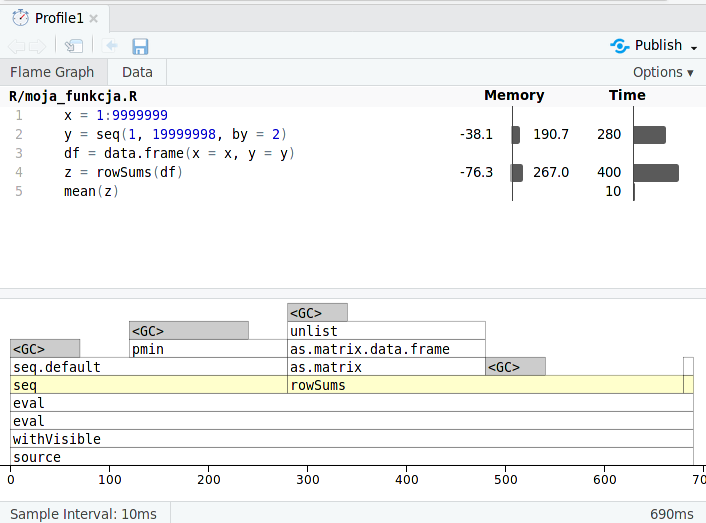
\includegraphics[width=\textwidth]{images/profvis} 

}

\caption{Zrzut ekranu przedstawiający wynik działania funkcji profvis().}\label{fig:profvis}
\end{figure}

Czas wykonania tego przykładu wyniósł sumarycznie 690ms.
Pierwsza linia tworząca obiekt \texttt{x} została wykonana bardzo szybko - poniżej mierzalnego progu.
Stworzenie obiektu \texttt{y} w drugiej linii zajęło ok. 280ms.
Trzecia linia została wykonana również w czasie poniżej mierzalnego progu.
Wynika to z kwestii, że tworzenie tam ramki danych nie powoduje wykonania nowych, złożonych obliczeń.
Powstała ona jedynie poprzez przekazanie odpowiednich adresów w pamięci do obiektów \texttt{x} i \texttt{y}.
Najbardziej czasochłonną okazała się linia czwarta.
Wyliczenie sum wierszy i stworzenie obiektu \texttt{z} zabrało ok. 400ms.
Ostatnia linia, wyliczająca średnią, zabrała ok. 10ms.

\hypertarget{benchmarking}{%
\section{Benchmarking}\label{benchmarking}}

Benchmarking oznacza określanie wydajności danej operacji czy funkcji.
Wydajność może być określona na wiele różnych sposobów, w tym najprostszym jest czas wykonania pewnego kodu.
Do określenia ile czasu zajmuje działanie operacji można użyć wbudowanej funkcji \texttt{system.time()}.

\begin{Shaded}
\begin{Highlighting}[]
\KeywordTok{system.time}\NormalTok{(kod_do_wykonania)}
\end{Highlighting}
\end{Shaded}

Przykładowo, poniżej nastąpi sprawdzenie czasu jaki zajmie wyliczenie średniej wartości z sekwencji od 1 do 100000000.

\begin{Shaded}
\begin{Highlighting}[]
\KeywordTok{system.time}\NormalTok{(}\KeywordTok{mean}\NormalTok{(}\DecValTok{1}\OperatorTok{:}\DecValTok{100000000}\NormalTok{))}
\CommentTok{#>    user  system elapsed }
\CommentTok{#>     0.5     0.0     0.5}
\end{Highlighting}
\end{Shaded}

W efekcie dostajemy trzy wartości - \texttt{user}, \texttt{system} i \texttt{elapsed}. Pierwsza z nich określa czas obliczenia po stronie użytkownika (sesji R), druga opisuje czas obliczenia po stronie systemu operacyjnego (np. otwieranie plików), a trzecia to sumaryczny czas wykonywania operacji.

Benchmarking jest często używany w sytuacji, gdy istnieje kilka funkcji służących do tego samego celu (np. w różnych pakietach) i chcemy znaleźć tę, która ma najwyższą wydajność.
Jest on też stosowany, gdy sami napisaliśmy kilka implementacji rozwiązania tego samego problemu i chcemy sprawdzić, które z nich jest najszybsze.

W sekcji \ref{for-example} stworzyliśmy kilka wersji pętli \texttt{for} pozwalającej na przeliczanie wartości z mil lądowych na kilometry.
Pierwsza z nich, tutaj zdefiniowana jako funkcja \texttt{mi\_do\_km1}, tworzy pusty wektor o długości 0, do którego następie doklejane są kolejne przeliczone wartości.

\begin{Shaded}
\begin{Highlighting}[]
\NormalTok{mi_do_km1 =}\StringTok{ }\ControlFlowTok{function}\NormalTok{(odl_mile)\{}
\NormalTok{  odl_km =}\StringTok{ }\KeywordTok{vector}\NormalTok{(}\StringTok{"list"}\NormalTok{, }\DataTypeTok{length =} \DecValTok{0}\NormalTok{)}
  \ControlFlowTok{for}\NormalTok{ (i }\ControlFlowTok{in} \KeywordTok{seq_along}\NormalTok{(odl_mile)) \{}
\NormalTok{    odl_km =}\StringTok{ }\KeywordTok{c}\NormalTok{(odl_km, odl_mile[[i]] }\OperatorTok{*}\StringTok{ }\FloatTok{1.609}\NormalTok{)}
\NormalTok{  \}}
\NormalTok{  odl_km}
\NormalTok{\}}
\end{Highlighting}
\end{Shaded}

Druga, tutaj zdefiniowana jako funkcja \texttt{mi\_do\_km2}, tworzy pusty wektor o oczekiwanej długości wyniku.
Następnie kolejne przeliczone wartości są wstawiane w odpowiednie miejsca wektora wynikowego.

\begin{Shaded}
\begin{Highlighting}[]
\NormalTok{mi_do_km2 =}\StringTok{ }\ControlFlowTok{function}\NormalTok{(odl_mile)\{}
\NormalTok{  odl_km =}\StringTok{ }\KeywordTok{vector}\NormalTok{(}\StringTok{"list"}\NormalTok{, }\DataTypeTok{length =} \KeywordTok{length}\NormalTok{(odl_mile))}
  \ControlFlowTok{for}\NormalTok{ (i }\ControlFlowTok{in} \KeywordTok{seq_along}\NormalTok{(odl_mile)) \{}
\NormalTok{    odl_km[[i]] =}\StringTok{ }\NormalTok{odl_mile[[i]] }\OperatorTok{*}\StringTok{ }\FloatTok{1.609}
\NormalTok{  \}}
\NormalTok{  odl_km}
\NormalTok{\}}
\end{Highlighting}
\end{Shaded}

Dwie powyższe funkcje można porównać używając \texttt{system.time()}.
Nie zawsze jednak to wystarczy - ta sama funkcja wykonana dwa razy może mieć różny czas obliczeń.
Dodatkowo, oprócz czasu wykonywania funkcji może nas interesować zużycie zasobów, takich jak pamięć operacyjna.
Do takiego celu powstała funkcja \texttt{mark()} z pakietu \textbf{bench} \citep{R-bench}, która wykonuje funkcje wiele razy przed zwróceniem wyniku.

Przyjmuje ona wywołania funkcji, które chcemy porównać.
Poniżej nastąpi porównanie funkcji \texttt{mi\_do\_km1} i \texttt{mi\_do\_km2}, w przypadku gdy jako dane wejściowe zostanie podana lista z wartościami 142, 63, 121.

\begin{Shaded}
\begin{Highlighting}[]
\KeywordTok{library}\NormalTok{(bench)}
\NormalTok{odl_mile =}\StringTok{ }\KeywordTok{list}\NormalTok{(}\DecValTok{142}\NormalTok{, }\DecValTok{63}\NormalTok{, }\DecValTok{121}\NormalTok{)}
\NormalTok{wynik_}\DecValTok{1}\NormalTok{ =}\StringTok{ }\KeywordTok{mark}\NormalTok{(}
  \KeywordTok{mi_do_km1}\NormalTok{(odl_mile),}
  \KeywordTok{mi_do_km2}\NormalTok{(odl_mile)}
\NormalTok{)}
\NormalTok{wynik_}\DecValTok{1}
\CommentTok{#> # A tibble: 2 x 6}
\CommentTok{#>   expression             min median `itr/sec` mem_alloc}
\CommentTok{#>   <bch:expr>          <bch:> <bch:>     <dbl> <bch:byt>}
\CommentTok{#> 1 mi_do_km1(odl_mile) 1.49us 1.67us   510468.     117KB}
\CommentTok{#> 2 mi_do_km2(odl_mile) 1.16us 1.33us   673544.     224KB}
\CommentTok{#> # ... with 1 more variable: `gc/sec` <dbl>}
\end{Highlighting}
\end{Shaded}

Efektem porównania jest ramka danych, w której każdy wiersz oznacza inną porównywaną funkcję.
Zawiera ona szereg charakterystyk, w tym:

\begin{itemize}
\tightlist
\item
  \texttt{min} - minimalny czas wykonania funkcji
\item
  \texttt{mean} - średni czas wykonania funkcji
\item
  \texttt{median} - mediana czasu wykonania funkcji
\item
  \texttt{max} - maksymalny czas wykonania funkcji
\item
  \texttt{itr/sec} - liczba wykonań funkcji na sekundę
\item
  \texttt{mem\_alloc} - pamięć użyta przez wywołanie funkcji
\item
  \texttt{n\_itr} - liczba powtórzeń wywołania funkcji
\end{itemize}

Wynik działania funkcji \texttt{mark()} pozwala na zauważenie, że na tym przykładzie funkcja \texttt{mi\_do\_km2} jest ok. 30\% szybsza od \texttt{mi\_do\_km1}.
Czasami możliwe jest, że jakaś funkcja działa relatywnie szybko na małych danych, ale dużo wolniej na większych danych wejściowych.
Warto jest więc sprawdzić, jak będzie wyglądało nasze porównanie na większej liście, np. z wartościami od 0 do 10000 co 1.

\begin{Shaded}
\begin{Highlighting}[]
\NormalTok{odl_mile2 =}\StringTok{ }\KeywordTok{as.list}\NormalTok{(}\DecValTok{0}\OperatorTok{:}\DecValTok{10000}\NormalTok{)}
\NormalTok{wynik_}\DecValTok{2}\NormalTok{ =}\StringTok{ }\KeywordTok{mark}\NormalTok{(}
  \KeywordTok{mi_do_km1}\NormalTok{(odl_mile2),}
  \KeywordTok{mi_do_km2}\NormalTok{(odl_mile2)}
\NormalTok{)}
\CommentTok{#> Warning: Some expressions had a GC in every iteration;}
\CommentTok{#> so filtering is disabled.}
\NormalTok{wynik_}\DecValTok{2}
\CommentTok{#> # A tibble: 2 x 6}
\CommentTok{#>   expression             min median `itr/sec` mem_alloc}
\CommentTok{#>   <bch:expr>           <bch> <bch:>     <dbl> <bch:byt>}
\CommentTok{#> 1 mi_do_km1(odl_mile2) 538ms  538ms      1.86     382MB}
\CommentTok{#> 2 mi_do_km2(odl_mile2) 801us  826us   1100.      78.2KB}
\CommentTok{#> # ... with 1 more variable: `gc/sec` <dbl>}
\end{Highlighting}
\end{Shaded}

W tym przypadku różnica pomiędzy \texttt{mi\_do\_km1} a \texttt{mi\_do\_km2} staje się dużo większa.
Funkcja \texttt{mi\_do\_km1} jest w stanie wykonać tylko 1.86 operacji na sekundę, przy aż 1100.37 operacji na sekundę funkcji \texttt{mi\_do\_km2}.
Dodatkowo, funkcja \texttt{mi\_do\_km1} potrzebowała aż kilka tysięcy (!) razy więcej pamięci operacyjnej niż \texttt{mi\_do\_km2}.

\hypertarget{zadania}{%
\section{Zadania}\label{zadania}}

\begin{Shaded}
\begin{Highlighting}[]
\KeywordTok{set.seed}\NormalTok{(}\DecValTok{2019-05-08}\NormalTok{)}
\NormalTok{mat =}\StringTok{ }\KeywordTok{matrix}\NormalTok{(}\KeywordTok{c}\NormalTok{(}\KeywordTok{sample}\NormalTok{(}\DecValTok{1}\OperatorTok{:}\DecValTok{10}\NormalTok{, }\DataTypeTok{size =} \DecValTok{25}\NormalTok{, }\DataTypeTok{replace =} \OtherTok{TRUE}\NormalTok{)),}
             \DataTypeTok{ncol =} \DecValTok{5}\NormalTok{, }\DataTypeTok{nrow =} \DecValTok{5}\NormalTok{)}
\NormalTok{mat}
\CommentTok{#>      [,1] [,2] [,3] [,4] [,5]}
\CommentTok{#> [1,]    6    1    2    4    6}
\CommentTok{#> [2,]    9    9    9    5    5}
\CommentTok{#> [3,]    2    6    4    8   10}
\CommentTok{#> [4,]    4    6    1    2    5}
\CommentTok{#> [5,]    2   10    6    4    9}
\end{Highlighting}
\end{Shaded}

\begin{enumerate}
\def\labelenumi{\arabic{enumi})}
\item
  Korzystając z wiedzy z rozdziału \ref{petle} dotyczącej pętli \texttt{for}, napisz funkcję \texttt{gdzie\_naj()}, która przyjmuje na wejściu macierz z wartościami numerycznymi, wylicza sumę wartości dla każdego wiersza, a następnie zwraca numer wiersza z najwyższą sumą wartości.
  Przykładowe dane wejściowe do tej funkcji znajdują się~nad tym zadaniem.
\item
  Dodaj do powyższej funkcji odpowiednie komunikaty błędów czy ostrzeżeń (sekcja \ref{obsluga-komunikatow}), pojawiające się~w zależności od rodzaju wprowadzonych danych wejściowych.
\item
  Napisz testy jednostkowe sprawdzające (1) czy błędy pojawiają się~w odpowiednich sytuacjach oraz (2) czy funkcja zwraca prawidłową wartość.
\item
  Użyj metod profilowania kodu w celu sprawdzenia czasów wykonywania kolejnych linii kodu.
  Działanie której linii kodu zabiera najwięcej czasu?
\item
  Stwórz funkcję \texttt{gdzie\_naj2()}, której cel jest taki sam jak funkcji \texttt{gdzie\_naj()}, ale zamiast pętli \texttt{for} jej działanie oparte jest o funkcję \texttt{rowSums()}.
\item
  Używając pakietu \textbf{bench} porównaj czas działania funkcji \texttt{gdzie\_naj()} i \texttt{gdzie\_naj2()}.
  Która z nich jest szybsza?
  Która z nich zużywa mniej zasobów?
\end{enumerate}

\hypertarget{debugging}{%
\chapter{Debugowanie}\label{debugging}}

Używając pakietów i funkcji stworzonych przez inne osoby możemy czasem znaleźć się w sytuacji, gdy zamiast wyniku otrzymujemy komunikat błędu.
Warto wówczas upewnić się czy nie napisaliśmy żadnej literówki i podaliśmy odpowiednie argumenty funkcji.
Konieczne kolejne kroki mogą obejmować sprawdzenie pliku pomocy danej funkcji, czy też skopiowanie najważniejszego fragmentu błędu i wklejenie go do wyszukiwarki internetowej.
Istnieje szansa, że ktoś już wcześniej napotkał ten problem, zadał pytanie i otrzymał na nie odpowiedź w internecie (np, na \url{https://stackoverflow.com/}).

Czasem się może jednak okazać, że odkryliśmy nowy problem - warto go wtedy zgłosić do twórców pakietu.
Wiele pakietów na platformie CRAN zawiera sekcję \emph{BugReports}, gdzie można znaleźć link do zgłaszania błędów.
Przykładowo, pakiet \textbf{stringr} jest opisany pod adresem \url{https://cran.r-project.org/package=stringr} i w jego sekcji \emph{BugReports} znajduje się odnośnik do \url{https://github.com/tidyverse/stringr/issues}.
W przypadku zgłaszania błędów zazwyczaj nie należy pisać bardzo długich opisów czy wklejać cały kod, który został napisany.
Konieczne jest natomiast przygotowanie powtarzalnego przykładu (ang. \emph{reproducible example}), czyli minimalnego kodu możliwego do odtworzenia problemu na innym komputerze (sekcja \ref{reprex}).
Warto jednak pamiętać, że sekcja \emph{Issue} na platformie Github służy głównie do zgłaszania problemów, a nie do zadawania pytań.
W przypadku potrzeby zadania pytania, lepszym pomysłem jest opublikowanie go na \url{https://stackoverflow.com/},

Tworzenie kodu możliwego do odtworzenia problemu (powtarzalnych przykładów) jest też pomocne w przypadku, gdy my piszemy nowe skrypty i funkcje i napotkamy na błędy.
Jest to często część debugowania (ang. \emph{debugging}) - procesu rozwiązywania problemów i błędów w oprogramowaniu.
Istnieje wiele potencjalnych taktyk debugowania kodu, w tym debugowanie używając funkcji takich jak \texttt{print()} (sekcja \ref{debuging-print}), czy też debuggera (sekcja \ref{debugger}).

Więcej na temat debugowania kodu w R można dowiedzieć się więcej z prezentacji Jenny Bryan pt. \href{https://github.com/jennybc/debugging}{Object of type `closure' is not subsettable}, \href{https://rstats.wtf/debugging-r-code.html}{rozdziału Debugging R code} książki \citet{rstatswtf}, oraz \href{https://adv-r.hadley.nz/debugging.html}{rozdziału Debugging} książki \citet{wickham2016r}.
Dodatkowo, na stronach \href{https://blog.davisvaughan.com/2019/04/05/debug-r-package-with-cpp/}{Debugging an R Package with C++}, \href{https://github.com/wch/r-debug/blob/master/debugging-r.md}{Debugging C/C++ code that interfaces with R}, oraz \href{http://kevinushey.github.io/blog/2015/04/13/debugging-with-lldb/}{Debugging with LLDB} można przeczytać na temat debugowania kodu C++ łączącego się z R.

\hypertarget{reprex}{%
\section{Powtarzalne przykłady}\label{reprex}}

Powtarzalny przykład oznacza fragment kodu, który może być odtworzony przez inną osobę na innym komputerze lub przez siebie samego w przyszłości.
Może on służyć pokazaniu poprawnego rozwiązania, wskazaniu na błędy w funkcjach, lub też jako załącznik do prośby o pomoc z kodem.
Powtarzalny przykład powinien składać się przynajmniej z:

\begin{itemize}
\tightlist
\item
  Z małego zbioru danych lub obiektu zawierającego dane wystarczającego do odtworzenia obliczeń
\item
  Krótkiego kodu, który może być uruchomiony na powyższym zbiorze danych
\end{itemize}

Czasem ważne są też dodatkowe informacje o używanej wersji R, posiadanym systemie operacyjnym, wersjach używanych pakietów, etc.
Można do tego użyć funkcji \texttt{sessionInfo()}.

\hypertarget{pakiet-reprex}{%
\subsection{\texorpdfstring{Pakiet \textbf{reprex}}{Pakiet reprex}}\label{pakiet-reprex}}

Stworzenie powtarzalnego przykładu w R może zostać ułatwione używając pakietu \textbf{reprex} \citep{R-reprex}.
Ten pakiet uruchamia wybraną część kodu w nowej sesji R uruchomionej w tle, wykonuje kolejne operacje, a następnie zapisuje uzyskany wynik do schowka.

Główną funkcją w tym pakiecie jest \texttt{reprex()}.
Funkcję \texttt{reprex()} można użyć poprzez wpisanie kodu wewnątrz tej funkcji lub też poprzez wybranie opcji \texttt{Reprex\ selection} z menu Addins w RStudio.
Możliwe jest również stworzenie powtarzalnego przykładu na podstawie skryptu R:

\begin{Shaded}
\begin{Highlighting}[]
\KeywordTok{reprex}\NormalTok{(}\DataTypeTok{input =} \StringTok{"moj_skrypt.R"}\NormalTok{)}
\end{Highlighting}
\end{Shaded}

Więcej informacji na temat powtarzalnych przykładów oraz pakietu \textbf{reprex} można znaleźć na \href{https://reprex.tidyverse.org/index.html}{oficjalnej stronie pakietu reprex}, oraz stronach \href{https://www.jessemaegan.com/post/so-you-ve-been-asked-to-make-a-reprex/}{So you've been asked to make a reprex}, \href{https://stackoverflow.com/questions/5963269/how-to-make-a-great-r-reproducible-example}{How to make a great R reproducible example}, \href{https://www.njtierney.com/post/2017/01/11/magic-reprex/}{Magic reprex}, \href{https://speakerdeck.com/jennybc/reprex-help-me-help-you}{reprex: help me help you!}, oraz \href{https://www.tidyverse.org/help/\#reprex}{Get help!}.

\hypertarget{tworzenie-powtarzalnego-przykux142adu}{%
\subsection{Tworzenie powtarzalnego przykładu}\label{tworzenie-powtarzalnego-przykux142adu}}

Działanie pakietu \textbf{reprex} można zobaczyć poniżej.
Tworzymy dwa obiekty \texttt{x} i \texttt{y}, przypisujemy im wartości, a następnie je mnożymy przez siebie.

\begin{Shaded}
\begin{Highlighting}[]
\NormalTok{x =}\StringTok{ }\DecValTok{1}
\NormalTok{y =}\StringTok{ }\DecValTok{5}
\NormalTok{x }\OperatorTok{*}\StringTok{ }\NormalTok{y}
\CommentTok{#> [1] 5}
\end{Highlighting}
\end{Shaded}

Ten sam kod umieszczony w funkcji \texttt{reprex()} wygląda w ten sposób:

\begin{Shaded}
\begin{Highlighting}[]
\KeywordTok{library}\NormalTok{(reprex)}
\KeywordTok{reprex}\NormalTok{(\{}
\NormalTok{  x =}\StringTok{ }\DecValTok{1}
\NormalTok{  y =}\StringTok{ }\DecValTok{5}
\NormalTok{  x }\OperatorTok{*}\StringTok{ }\NormalTok{y}
\NormalTok{\})}
\end{Highlighting}
\end{Shaded}

Wynik działania powyższego kodu zapisywany jest w schowku jako Markdown oraz w postaci wyświetlonego pliku HTML:

\begin{center}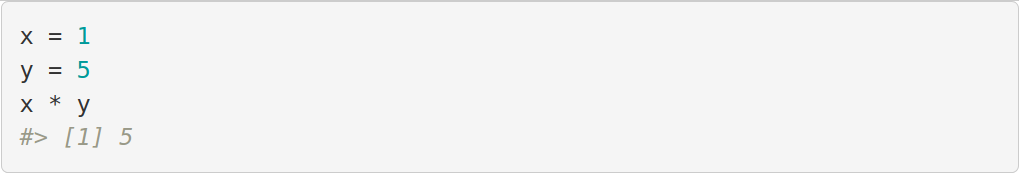
\includegraphics[width=\textwidth]{figures/reprex1} \end{center}

Kolejny powtarzalny przykład pochodzi z rozdziału \ref{tekst}, gdzie naszym celem było określenie które elementy wektora \texttt{tekst3} rozpoczynają się od dużej litery \texttt{L}.

\begin{Shaded}
\begin{Highlighting}[]
\KeywordTok{reprex}\NormalTok{(\{}
\NormalTok{  teskt3 =}\StringTok{ }\KeywordTok{c}\NormalTok{(}\StringTok{"Magdalena"}\NormalTok{, }\StringTok{"Lena"}\NormalTok{, }\StringTok{"1Lena.csv"}\NormalTok{, }\StringTok{"LLena"}\NormalTok{, }\StringTok{"Helena"}\NormalTok{, }\StringTok{"Anna"}\NormalTok{, }\StringTok{"99"}\NormalTok{)}
  \KeywordTok{str_detect}\NormalTok{(tekst3, }\DataTypeTok{pattern =} \StringTok{"^L"}\NormalTok{)}
\NormalTok{\})}
\end{Highlighting}
\end{Shaded}

Niestety zwraca on błąd.
Powyższy kod ma dwa problemy - czy jesteś w stanie je wskazać?

\begin{center}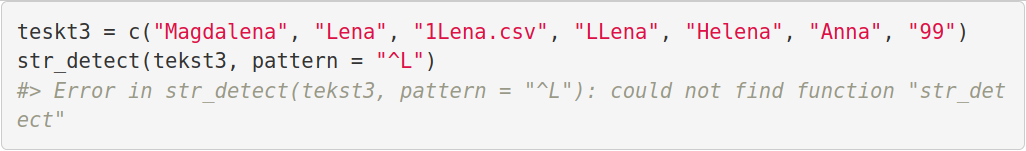
\includegraphics[width=\textwidth]{figures/reprex2} \end{center}

Odpowiedź - ten kod nie jest w pełni samowystarczalny - brakuje tam dołączenia pakietu \textbf{stringr}, który zawiera funkcję \texttt{str\_detect()}.
Drugi problem to literówka w obiekcie \texttt{teskt3}.
Naprawiona wersja tego kodu znajduje się poniżej:

\begin{Shaded}
\begin{Highlighting}[]
\KeywordTok{reprex}\NormalTok{(\{}
  \KeywordTok{library}\NormalTok{(stringr)}
\NormalTok{  tekst3 =}\StringTok{ }\KeywordTok{c}\NormalTok{(}\StringTok{"Magdalena"}\NormalTok{, }\StringTok{"Lena"}\NormalTok{, }\StringTok{"1Lena.csv"}\NormalTok{, }\StringTok{"LLena"}\NormalTok{, }\StringTok{"Helena"}\NormalTok{, }\StringTok{"Anna"}\NormalTok{, }\StringTok{"99"}\NormalTok{)}
  \KeywordTok{str_detect}\NormalTok{(tekst3, }\DataTypeTok{pattern =} \StringTok{"^L"}\NormalTok{)}
\NormalTok{\})}
\end{Highlighting}
\end{Shaded}

\begin{center}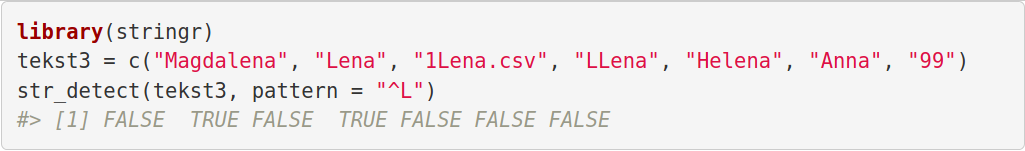
\includegraphics[width=\textwidth]{figures/reprex3} \end{center}

\hypertarget{proces-debugowania}{%
\section{Proces debugowania}\label{proces-debugowania}}

Nie ma uniwersalnego procesu debugowania, który działa dla każdego napotkanego problemu programistycznego.
Można jednak określić kilka kroków, które mogą znacząco ułatwić debugowanie:

\begin{enumerate}
\def\labelenumi{\arabic{enumi}.}
\tightlist
\item
  Powtarzalność błędu
\item
  Identyfikacja przyczyny błędu
\item
  Usunięcie błędu
\item
  Weryfikacja naprawy błędu i jej konsekwencji
\end{enumerate}

W pierwszym kroku warto się upewnić, że napotkany błąd nie jest spowodowany przez inne obiekty w środowisku R.
Należy wyczyścić środowisko R używając \texttt{rm(list\ =\ ls())} a następnie zresetować sesję R (skrót CTRL+SHIFT+F10 w RStudio).
Warto też wydzielić z kodu najmniejszy fragment, który pozwala na odtworzenie błędu (\emph{powtarzalny przykład}).
Teraz należy jeszcze raz spróbować użyć kodu zwracającego błąd, aby się upewnić, że dalej istnieje.
Drugi krok obejmuje zlokalizowanie dokładnego miejsca w którym błąd powstaje.
Może to być konkretna linia kodu, miejsce w pętli, a czasem nawet wywołanie innej zewnętrznej funkcji.
Ten krok można wykonać na wiele sposobów.
Dwa z nich, debugowanie używając funkcji takich jak print (sekcja \ref{debuging-print}) i debugowanie interaktywne (sekcja \ref{debugger}), są opisane w tym rozdziale.
W trzecim kroku należy usunąć wcześniej zlokalizowany błąd.
Nie powinien to być jednak ostatni krok.
Należy jeszcze upewnić się, że nowa wersja kodu nie tylko przestaje zwracać błędy, ale też daje poprawne wyniki.
Często odbywa się to poprzez wykonanie wcześniej stworzony testów jednostkowych (sekcja \ref{testy-jednostkowe}).

\hypertarget{debuging-print}{%
\section{Podstawowe podejście do debugowania}\label{debuging-print}}

Klasycznym podejściem do debugowania jest dodanie funkcji \texttt{print()} pokazującej wartości obiektów w okolicy linii kodu, którą uznajemy za potencjalne źródło błędu.
Dalej warto zaplanować jakie testy kodu wykonać, aby wyłapać dokładne miejsce wystąpnienia błędu.
Trzeba też zapisywać potencjalne wyniki.
Takie systematyczne podejście może zaoszczędzić dużo czasu w porównaniu do losowego testowania różnych wartości w kodzie.

Oprócz funkcji \texttt{print()} można też wykorzystać funkcję \texttt{cat()} w przypadku małych obiektów lub funkcję \texttt{str()} w przypadku większych obiektów.

\hypertarget{debugger}{%
\section{Debugger}\label{debugger}}

R posiada także wbudowany debugger - program analizujący kod w celu odnalezienia zawartych w nim błędów.
Pozwala on na wejście do środka wykonywanych funkcji, śledzenie i edycję wartości poszczególnych obiektów oraz wykonywanie kodu linia po linii.

Dla przykładu stwórzmy nową funkcję \texttt{f\_to\_c()}, która zamienia wartości ze stopni Fahrenheita na stopnie Celsjusza.
Dodatkowo sprawdza ona czy podana wartość (argument \texttt{x}) nie jest numeryczna oraz czy jest mniejsza niż zero i w takich wypadkach wywołuje ona błąd.

\begin{Shaded}
\begin{Highlighting}[]
\NormalTok{f_to_c =}\StringTok{ }\ControlFlowTok{function}\NormalTok{(x) \{}
  \ControlFlowTok{if}\NormalTok{ (}\OperatorTok{!}\KeywordTok{is.numeric}\NormalTok{(x))\{}
    \KeywordTok{stop}\NormalTok{(}\StringTok{"Podana wartość nie jest numeryczna"}\NormalTok{)}
\NormalTok{  \}}
  \ControlFlowTok{if}\NormalTok{ (x }\OperatorTok{<}\StringTok{ }\DecValTok{0}\NormalTok{)\{}
    \KeywordTok{stop}\NormalTok{(}\StringTok{"Wartość poniżej 0 nie jest możliwa")}
\StringTok{  \}}
\StringTok{  y = x - 32}
\StringTok{  y = y / 1.8}
\StringTok{  y}
\StringTok{\}}
\end{Highlighting}
\end{Shaded}

Dodatkowo, wyobraźmy sobie, że funkcja \texttt{f\_to\_c()} jest używana w obliczeniach jakiejś kolejnej funkcji \texttt{fun1()}, która jest używana w obliczeniach funkcji \texttt{fun2()}, a ta w funkcji \texttt{fun3()}.

\begin{Shaded}
\begin{Highlighting}[]
\NormalTok{fun1 =}\StringTok{ }\ControlFlowTok{function}\NormalTok{(x)\{}
  \KeywordTok{f_to_c}\NormalTok{(x)}
\NormalTok{\}}
\NormalTok{fun2 =}\StringTok{ }\ControlFlowTok{function}\NormalTok{(x)\{}
  \KeywordTok{fun1}\NormalTok{(x)}
\NormalTok{\}}
\NormalTok{fun3 =}\StringTok{ }\ControlFlowTok{function}\NormalTok{(x)\{}
  \KeywordTok{fun2}\NormalTok{(x)}
\NormalTok{\}}
\end{Highlighting}
\end{Shaded}

Powyższe funkcje jedynie wywołują siebie nawzajem, ale w typowej sytuacji składałyby się one z wielu linii kodu i wykonywałby szereg operacji.
Załóżmy teraz, że chcemy wykonać i otrzymać wynik działania \texttt{fun3()} dla podanego argumentu \texttt{1}.

\begin{Shaded}
\begin{Highlighting}[]
\KeywordTok{fun3}\NormalTok{(}\DecValTok{1}\NormalTok{)}
\CommentTok{#> [1] -17.2}
\end{Highlighting}
\end{Shaded}

W tym przypadku po chwili otrzymujemy poprawny wynik -17.2.
Możliwa jest jednak sytuacja, gdy my, nasi użytkownicy, albo inny program poda na wejściu wartość, która kończy się błędem, np. \texttt{-1}.

\begin{Shaded}
\begin{Highlighting}[]
\KeywordTok{fun3}\NormalTok{(}\OperatorTok{-}\DecValTok{1}\NormalTok{)}
\CommentTok{#> Error in f_to_c(x): Wartość poniżej 0 nie jest możliwa}
\end{Highlighting}
\end{Shaded}

Otrzymujemy komunikat błędu, ale nie wiemy wynikiem działania jakiej funkcji jest ten błąd.
Przykładowo, chcemy zezwolić naszym użytkownikom na podawanie wartości ujemnych - musimy poprawić jakieś miejsce w kodzie, ale nie wiemy gdzie.
Z pomocą tutaj może przyjść funkcja \texttt{traceback()}.

\begin{Shaded}
\begin{Highlighting}[]
\KeywordTok{traceback}\NormalTok{()}
\CommentTok{#> 3: stop("Wartość poniżej 0 nie jest możliwa") at #3}
\CommentTok{#> 2: inch_to_mm(x) at #2}
\CommentTok{#> 1: fun3(-1)}
\end{Highlighting}
\end{Shaded}

Czytamy jej wynik od dołu do góry, dowiadując się, że wywołanie funkcji \texttt{fun3(-1)} skończyło się błędem wewnątrz funkcji \texttt{f\_to\_c(x)}, a dokładnie w linii \texttt{stop("Wartość\ poniżej\ 0\ nie\ jest\ możliwa")}.
Posiadając tę wiedzę możemy przejść do funkcji \texttt{f\_to\_c()} i zmienić ją zgodnie z naszymi potrzebami.

Alternatywną możliwością do funkcji \texttt{traceback()} jest włączenie opcji interaktywnego debuggera w RStudio.
Pierwszym krokiem jest włączenie tzw. Error Inspectora, co można zrobić w menu RStudio \texttt{Debug\ -\textgreater{}\ On\ Error\ -\textgreater{}\ Error\ Inspector}.
Teraz po wykonaniu kodu \texttt{fun3(-1)} otrzymamy nie tylko komunikat błędu, ale także dwie nowe ikony \texttt{Show\ Traceback} i \texttt{Rerun\ with\ Debug}.

\begin{center}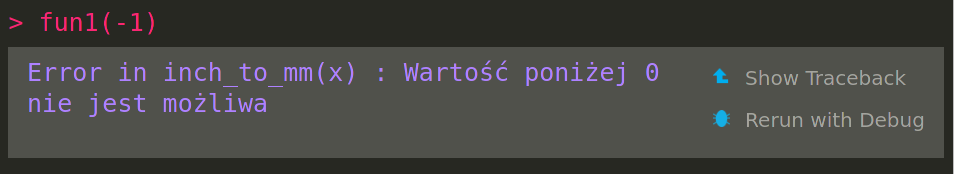
\includegraphics[width=\textwidth]{figures/debugger1} \end{center}

Pierwsza z nich wywołuje działanie wcześniej opisanej funkcji \texttt{traceback()}.
Druga, \texttt{Rerun\ with\ Debug}, uruchamia interaktywny debugger.
W tym momencie cały kod jest ponownie wykonywany i zatrzymywany w miejscu gdzie błąd powstał.
Teraz w oknie Environment można znaleźć dwie grupy informacji: istniejące obiekty oraz Traceback pokazujący w którym kroku obliczeń jesteśmy.
Dodatkowo konsola R wygląda inaczej niż zwykle.
Pod informacją o błędzie wyświetlił się tekst \texttt{Browse{[}1{]}\textgreater{}}, a nad oknem konsoli pojawił się szereg ikon:

\begin{center}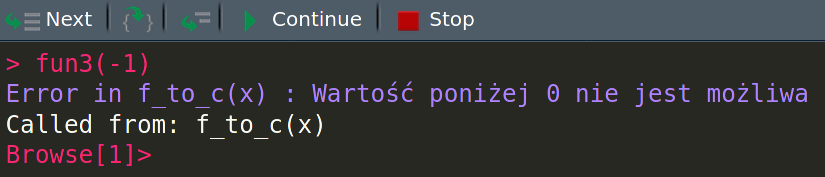
\includegraphics[width=\textwidth]{figures/debugger2} \end{center}

\begin{itemize}
\tightlist
\item
  Pierwsza ikona \texttt{Next}, skrót klawiaturowy \texttt{n}, wykonuje kolejny krok obliczeń
\item
  Druga ikona, \texttt{s}, działa podobnie do \texttt{Next}, z tym wyjątkiem, że gdy kolejny krok obliczeń jest funkcją to wtedy pozwala ona na wejście do tej funkcji i sprawdzenie jej interaktywnie
\item
  Trzecia ikona, \texttt{f}, kończy działanie obecnej funkcji lub pętli
\item
  Czwarta ikona, \texttt{c}, wyłącza interaktywny debugger ale pozwala na dalsze wykonywanie działań wewnątrz funkcji
\item
  Ostatnia ikona, \texttt{Q}, kończy działanie debuggera
\end{itemize}

Uzyskane informacje z debuggera pozwalają nie tylko na zrozumienie, gdzie jest miejsce w którym błąd się pojawia, ale także jakie są wtedy wartości naszych obiektów.
Teraz w konsoli możemy wpisać \texttt{ls.str()} co pozwala sprawdzić jakie obiekty znajdują się w pamięci komputera w tej sesji R.
Możemy się o tym też dowiedzieć w oknie Environment.

Domyślnie interaktywny debugger aktywowany jest w przypadku wywołania błędu.
Możemy go jednak zastosować, gdy chcemy się dowiedzieć jakie obiekty i ich wartości znajdują się w konkretnym miejscu działania naszej funkcji.
Wtedy konieczne jest zasygnalizowanie, gdzie chcemy aby debugger został aktywowany, co możemy zrobić na dwa podstawowe sposoby.
Pierwszy z nich polega na dodaniu przed interesującym nas miejscem linii kodu z funkcją \texttt{browser()}, druga natomiast polega na kliknięciu w RStudio na lewo od numeru interesującej nas linii kodu.
Wówczas pojawi się czerwona kropka, tzw. ``breakpoint'', sygnalizująca, że w tym miejscu zostanie uruchomiony debugger i będziemy mogli sprawdzić stan działania programu.
Inne możliwości wywołania interaktywnego debuggera dają takie funkcje jak \texttt{debug()}, \texttt{trace()} i \texttt{recover()}.\footnote{Wyjaśnienie działania tych funkcji można znaleźć w prezentacji Jima Hestera Introduction to debugging in R and RStudio, której nagranie jest pod adresem \url{https://www.youtube.com/watch?v=r7oBeEyN2jQ}}

\hypertarget{zadania}{%
\section{Zadania}\label{zadania}}

\begin{enumerate}
\def\labelenumi{\arabic{enumi}.}
\tightlist
\item
  Stwórz powtarzalny przykład pokazujący działanie funkcji \texttt{f\_to\_c()} na wartościach wejściowych \texttt{10} oraz \texttt{"ciepło"}.
\item
  Włącz Error Inspectora w RStudio na stałe (\texttt{Debug\ -\textgreater{}\ On\ Error\ -\textgreater{}\ Error\ Inspector}).
  Kolejny raz gdy pojawi się błąd w Twoim kodzie, użyj opcji \texttt{Show\ Traceback} i \texttt{Rerun\ with\ Debug}.
  Czy pomogło to w rozwiązaniu problemu?
\item
  Zapisz funkcję \texttt{f\_to\_c()} stworzoną w tym rozdziale do pliku \texttt{f\_to\_c.R}.
  Otwórz ten skrypt i ustaw ``breakpoint'' w linii \texttt{y\ =\ x\ -\ 32}.
  Uruchom tę funkcję i sprawdź co będzie tego efektem.
\end{enumerate}

\hypertarget{lacznik}{%
\chapter{Łącznik}\label{lacznik}}

R ma bezpośrednio wbudowane mechanizmy łączenia kodu R z kodem napisanym w językach C i Fortan.
W tym rozdziale skupimy się jednak na przykładach łączenia R z innymi, popularnymi współcześnie językami programowania C++ i Pythonem (sekcje \ref{cpp} i \ref{python}) oraz z systemową linią komend (sekcja \ref{powloka-systemowa}).
Inne możliwe połączenia R to z językami takimi jak \href{https://github.com/r-rust/hellorust}{Rust}, \href{https://jeroen.cran.dev/V8/}{JavaScript}, czy \href{http://www.rforge.net/rJava/}{Java}.

\hypertarget{cpp}{%
\section{C++}\label{cpp}}

C++ jest jednym z najczęściej używanych kompilowanych języków programowania.
Jest to spowodowane kilkoma zaletami tego języka, w tym jego wysoką wydajnością, niezależnością od konkretnej platformy systemowej, czy uniwersalnością.

Język C++ posiada zarówno wiele podobnych do R konstrukcji i koncepcji, ale też różni się w pewnych kluczowych koncepcjach.
Najważniejsze cechy C++, które wyróżniają go od R i które warto znać na początku:

\begin{itemize}
\tightlist
\item
  Jest językiem kompilowanym
\item
  Pozwala na używanie tylko \texttt{=} jako operatora przypisania
\item
  Zakłada głównie statyczną kontrolę typów
\item
  Posiada typ skalarny
\item
  Domyślnie nie używa wektoryzacji
\item
  Większość linii kodu należy kończyć znakiem średnika \texttt{;}
\item
  Konieczne jest zwracanie wartości używając \texttt{return}
\end{itemize}

Przykładowy kod R do przeliczania temperatury ze stopni Fahrenheita na Celsjusza wygląda w poniższy sposób (sekcja \ref{budowanie-funkcji}):

\begin{Shaded}
\begin{Highlighting}[]
\NormalTok{konwersja_temp =}\StringTok{ }\ControlFlowTok{function}\NormalTok{(temperatura_f)\{}
\NormalTok{    (temperatura_f }\OperatorTok{-}\StringTok{ }\DecValTok{32}\NormalTok{) }\OperatorTok{/}\StringTok{ }\FloatTok{1.8}
\NormalTok{\}}
\end{Highlighting}
\end{Shaded}

To samo obliczenie wykonane w języku C++ może wyglądać w ten sposób:

\begin{Shaded}
\begin{Highlighting}[]
\DataTypeTok{double}\NormalTok{ konwersja_temp_cpp(}\DataTypeTok{double}\NormalTok{ temperatura_f)\{}
  \DataTypeTok{double}\NormalTok{ temperatura_c = (temperatura_f - }\DecValTok{32}\NormalTok{) / }\FloatTok{1.8}\NormalTok{;}
  \ControlFlowTok{return}\NormalTok{ temperatura_c;}
\NormalTok{\}}
\end{Highlighting}
\end{Shaded}

Odnosząc się do punktów z wcześniej wymienionej listy:

\begin{itemize}
\tightlist
\item
  Jest językiem kompilowanym - gdybyśmy chcieli użyć powyższą funkcję jako program C++ musielibyśmy stworzyć kolejną funkcję \texttt{main()}, a następnie skompilować kod.
  Nie jest możliwe wykonywanie tego kodu linia po linii
\item
  Pozwala na używanie tylko \texttt{=} jako operatora przypisania - nie możemy w nim użyć operatora \texttt{\textless{}-} czy \texttt{-\textgreater{}}
\item
  Zakłada głównie statyczną kontrolę typów - w powyższym przykładzie musieliśmy zadeklarować, że nasza funkcja \texttt{konwersja\_temp\_cpp}, nasz argument \texttt{temperatura\_f} oraz zmienna \texttt{temperatura\_c} będzie typu \texttt{double}. Zrobiliśmy to poprzez dodanie nazwy typu przed nazwą funkcji/argumentu/zmiennej.
  Co ważne, w tym języku też typy (zazwyczaj) nie są automatycznie konwertowane do innych typów jak ma to miejsce w R (sekcja \ref{lpto-vector}).
\item
  Posiada typ skalarny - \texttt{double} może przechowywać tylko jedną wartość.
\item
  Domyślnie nie używa wektoryzacji - powyższa funkcja \texttt{konwersja\_temp\_cpp()} zwróci błąd \texttt{Expecting\ a\ single\ value} w przypadku podania wektora numerycznego jako obiekt wejściowy.
  Aby użyć wektor wartości na wejściu konieczne jest napisane pętli lub użycie innych podobnych konstrukcji.
\item
  Większość linii kodu należy kończyć znakiem średnika \texttt{;}.
  Nie dotyczy to linii definiujących powstanie funkcji, rozpoczynających i kończących pętle czy wyrażenia warunkowe
\item
  Konieczne jest zwracanie wartości używając \texttt{return}.
  W R użycie funkcji \texttt{return()} było opcjonalne.
\end{itemize}

Obecnie ponad dwa tysiące pakietów R łączy się z językiem C++ używając pakietu \textbf{Rcpp} \citep{R-Rcpp}.
Dodanie języka C++ do pakietu R często ma na celu przyspieszenie pewnych wymagających obliczeniowo zadań lub połączenie R z istniejącymi zewnętrznymi bibliotekami napisanymi w C++.

\begin{Shaded}
\begin{Highlighting}[]
\KeywordTok{library}\NormalTok{(Rcpp)}
\end{Highlighting}
\end{Shaded}

Pakiet \textbf{Rcpp} pozwala na zarówno wywoływanie kodu C++ wewnątrz skryptów R (sekcja \ref{cppFunction}), jak używając zewnętrznych plików o rozszerzeniu \texttt{.cpp} (sekcja \ref{sourceCpp}).

Ta część książki ma na celu pokazanie zupełnych podstaw łączenia R z C++.
Więcej informacji na ten temat można znaleść na stronie \url{http://www.rcpp.org/}, w \href{https://adv-r.hadley.nz/rcpp.html}{rozdziale Rewriting R code in C++} książki \citet{wickham2014advanced}, \href{https://csgillespie.github.io/efficientR/rcpp.html}{sekcji Rcpp} książki \citet{gillespie2016efficient}, oraz na stronie \href{https://thecoatlessprofessor.com/programming/cpp/unofficial-rcpp-api-documentation}{Unofficial Rcpp API Documentation}.

\hypertarget{cppFunction}{%
\subsection{Wywoływanie kodu C++ wewnątrz skryptu R}\label{cppFunction}}

W przypadku krótkich fragmentów kodu C++ możliwe jest umieszczenie ich wewnątrz skryptu R jako obiekt tekstowy.
Poniższej stworzono nowy obiekt \texttt{rcpp\_fun1}, który zawiera wcześniejszą funkcję C++.

\begin{Shaded}
\begin{Highlighting}[]
\NormalTok{rcpp_fun1 =}\StringTok{ "}
\StringTok{double konwersja_temp_cpp(double temperatura_f)\{}
\StringTok{  double temperatura_c = (temperatura_f - 32) / 1.8;}
\StringTok{  return temperatura_c;}
\StringTok{\}}
\StringTok{"}
\end{Highlighting}
\end{Shaded}

W kolejnym kroku konieczne jest skompilowanie powyższego kodu i stworzenie połączenia pomiędzy nim a R za pomocą funkcji \texttt{cppFunction()}.

\begin{Shaded}
\begin{Highlighting}[]
\KeywordTok{cppFunction}\NormalTok{(rcpp_fun1)}
\end{Highlighting}
\end{Shaded}

Od tego momentu możliwe jest korzystanie z funkcji \texttt{konwersja\_temp\_cpp()}.
Możemy sprawdzić jej działanie poprzez podanie wybranej przez nas wartości, na przykład \texttt{75}.

\begin{Shaded}
\begin{Highlighting}[]
\KeywordTok{konwersja_temp_cpp}\NormalTok{(}\DecValTok{75}\NormalTok{)}
\CommentTok{#> [1] 23.9}
\end{Highlighting}
\end{Shaded}

Warto jednak nadal pamiętać, że powyższa funkcja nie jest zwektoryzowana - możliwe jest podanie w niej tylko obiektu o długości 1.
W przypadku zadeklarowania dłuższego obiektu wejściowego otrzymamy błąd:

\begin{Shaded}
\begin{Highlighting}[]
\KeywordTok{konwersja_temp_cpp}\NormalTok{(}\KeywordTok{c}\NormalTok{(}\DecValTok{0}\NormalTok{, }\DecValTok{75}\NormalTok{, }\DecValTok{110}\NormalTok{))}
\CommentTok{#> Error in konwersja_temp_cpp(c(0, 75, 110)): Expecting a single value: [extent=3].}
\end{Highlighting}
\end{Shaded}

W sekcji \ref{zastosowanie-w-funkcjach} stworzyliśmy funkcję \texttt{mile\_na\_km()}, która przyjmuje i zwraca obiekt o klasie lista i zamienia wartości elementów tej listy z mil lądowych na kilometry.

\begin{Shaded}
\begin{Highlighting}[]
\NormalTok{mile_na_km =}\StringTok{ }\ControlFlowTok{function}\NormalTok{(odl_mile) \{}
\NormalTok{  odl_km =}\StringTok{ }\KeywordTok{vector}\NormalTok{(}\StringTok{"list"}\NormalTok{, }\DataTypeTok{length =} \KeywordTok{length}\NormalTok{(odl_mile))}
  \ControlFlowTok{for}\NormalTok{ (i }\ControlFlowTok{in} \KeywordTok{seq_along}\NormalTok{(odl_mile)) \{}
\NormalTok{    odl_km[[i]] =}\StringTok{ }\NormalTok{odl_mile[[i]] }\OperatorTok{*}\StringTok{ }\FloatTok{1.609}
\NormalTok{  \}}
\NormalTok{  odl_km}
\NormalTok{\}}
\end{Highlighting}
\end{Shaded}

Ta sama funkcja w języku C++ może wyglądać w ten sposób:

\begin{Shaded}
\begin{Highlighting}[]
\NormalTok{List mile_na_km_cpp(List odl_mile)\{}
  \DataTypeTok{int}\NormalTok{ odl_mile_len = odl_mile.size();}
\NormalTok{  List result(odl_mile_len);}
  \ControlFlowTok{for}\NormalTok{ (}\DataTypeTok{int}\NormalTok{ i = }\DecValTok{0}\NormalTok{; i < odl_mile_len; i++)\{}
\NormalTok{    result[i] = odl_mile[i] * }\FloatTok{1.609}\NormalTok{;}
\NormalTok{  \}}
  \ControlFlowTok{return}\NormalTok{ result;}
\NormalTok{\}}
\end{Highlighting}
\end{Shaded}

Zawiera ona szereg różnic od kodu R.
Oprócz definicji typów, używania średnika i operatora \texttt{return}, widać tutaj także inną metodę wywołania funkcji oraz inny sposób definiowania pętli \texttt{for}.

Zadaniem linii \texttt{int\ odl\_mile\_len\ =\ odl\_mile.size();} jest stworzenie nowej zmiennej skalarnej (\texttt{odl\_mile\_len}) o typie integer (\texttt{int}).
Ta nowa zmienna jest wynikiem działania funkcji \texttt{size()}, która jest odpowiednikiem używanej w R \texttt{length()}.
W przypadku używania R wywołanie funkcji ma jednak postać, w której podajemy nazwę funkcji, a następnie w nawiasie okrągłym obiekt wejściowy.
C++ pozwala też na inny sposób wywoływania funkcji - używając wbudowanych metod.
Odbywa się to poprzez podanie nazwy obiektu (\texttt{odl\_mile}), a następnie po kropce (\texttt{.}) podania nazwy funkcji (\texttt{size()}).

W C++ pętle można definiować używając poniższej składni:

\begin{Shaded}
\begin{Highlighting}[]
\ControlFlowTok{for}\NormalTok{ (inicjalizacja zmiennej; warunek zakończenia; aktualizacja zmiennej) \{}
  \CommentTok{// Kod do wykonania}
\NormalTok{\}}
\end{Highlighting}
\end{Shaded}

Po pierwsze należy przekazać w miejscu \texttt{inicjalizacja\ zmiennej} stworzenie zmiennej, na podstawie której będzie oparta pętla.
\texttt{int\ i\ =\ 0} oznacza, że tworzymy zmienną o typie integer \texttt{i}, która przyjmuje wartość 0.
Jest to spowodowane ważną różnicą między C++ a R - w tym pierwszym języku liczenie rozpoczynamy od 0.
Przykładowo w C++, \texttt{a{[}0{]}} pozwoli na wybranie pierwszego elementu z wektora \texttt{a}.
Drugim elementem jest \texttt{warunek\ trwania}, czyli określenie do kiedy pęlta trwa.
\texttt{i\ \textless{}\ odl\_mile\_len} oznacza, że pętla będzie działała tak długo aż \texttt{i} będzie mniejsze niż \texttt{odl\_mile\_len}.
Ostatni element, \texttt{aktualizacja\ zmiennej}, mówi co ma się stać ze stworzoną zmienną po każdym przebiegu pętli.
\texttt{i++} to skrót w języku C++ mówiący, że z każdą pętlą wartość \texttt{i} będzie rosła o 1.
Jest to odpowiednik kodu \texttt{i\ =\ i\ +\ 1}.

W powyższej składni też widać sposób definiowania komentarzy w języku C++, gdzie używa się operatora \texttt{//}.

Zainicjujmy funkcję C++ \texttt{mile\_na\_km\_cpp()} używając \texttt{cppFunction()}.

\begin{Shaded}
\begin{Highlighting}[]
\NormalTok{rcpp_fun2 =}\StringTok{ "List mile_na_km_cpp(List odl_mile)\{}
\StringTok{  int odl_mile_len = odl_mile.size();}
\StringTok{  List result(odl_mile_len);}
\StringTok{  for (int i = 0; i < odl_mile_len; i++)\{}
\StringTok{    result[i] = odl_mile[i] * 1.609;}
\StringTok{  \}}
\StringTok{  return result;}
\StringTok{\}"}
\KeywordTok{cppFunction}\NormalTok{(rcpp_fun2)}
\end{Highlighting}
\end{Shaded}

Możemy sprawdzić jej działanie na przykładowym wektore \texttt{odl\_mile} używając kodu poniżej.

\begin{Shaded}
\begin{Highlighting}[]
\NormalTok{odl_mile =}\StringTok{ }\KeywordTok{list}\NormalTok{(}\DecValTok{142}\NormalTok{, }\DecValTok{63}\NormalTok{, }\DecValTok{121}\NormalTok{)}
\KeywordTok{mile_na_km_cpp}\NormalTok{(odl_mile)}
\CommentTok{#> [[1]]}
\CommentTok{#> [1] 228}
\CommentTok{#> }
\CommentTok{#> [[2]]}
\CommentTok{#> [1] 101}
\CommentTok{#> }
\CommentTok{#> [[3]]}
\CommentTok{#> [1] 195}
\end{Highlighting}
\end{Shaded}

Dodatkowo warto porównać prędkość rozwiązania w R z C++ używająć listy o długości 10001 i funkcji \texttt{mark()} z pakietu \textbf{bench}.

\begin{Shaded}
\begin{Highlighting}[]
\NormalTok{odl_mile2 =}\StringTok{ }\KeywordTok{as.list}\NormalTok{(}\DecValTok{0}\OperatorTok{:}\DecValTok{10000}\NormalTok{)}
\NormalTok{wynik =}\StringTok{ }\NormalTok{bench}\OperatorTok{::}\KeywordTok{mark}\NormalTok{(}
  \KeywordTok{mile_na_km}\NormalTok{(odl_mile2),}
  \KeywordTok{mile_na_km_cpp}\NormalTok{(odl_mile2)}
\NormalTok{)}
\NormalTok{wynik}
\CommentTok{#> # A tibble: 2 x 6}
\CommentTok{#>   expression                  min median `itr/sec`}
\CommentTok{#>   <bch:expr>                <bch> <bch:>     <dbl>}
\CommentTok{#> 1 mile_na_km(odl_mile2)     815us  835us     1156.}
\CommentTok{#> 2 mile_na_km_cpp(odl_mile2) 432us  450us     2162.}
\CommentTok{#> # ... with 2 more variables: mem_alloc <bch:byt>,}
\CommentTok{#> #   `gc/sec` <dbl>}
\end{Highlighting}
\end{Shaded}

Mimo otrzymania tego samego wyniku, czas wykonania funkcji napisanej w C++ był około 1.85 raza mniejszy.

\hypertarget{sourceCpp}{%
\subsection{Wywoływanie kodu z plików .cpp}\label{sourceCpp}}

Powyższy przykład sprawdza się w przypadku małych fragmentów kodu C++.
W momencie jednak, gdy kod staje się bardziej złożony, znacznie lepsze jest umieszczenie go w oddzielnym pliku o rozszerzeniu \texttt{.cpp}.
Taki plik może też być umieszczony wewnątrz pakietu R (rozdział \ref{tworzenie-pakietow}).

Używanie kod C++ z pliku z poziomu R wymaga jednak pewnych dodatkowych działań.
Konieczne jest dodane do tego pliku kilku linii nagłówków, które umożliwią interakcję pomiędzy C++ a R.

Pierwsza z nich ma na celu umożliwienie dostępu do funkcji z pakietu \textbf{Rcpp}, poprzez podanie nazwy pliku \texttt{Rcpp.h} w linii \texttt{\#include}.

\begin{Shaded}
\begin{Highlighting}[]
\PreprocessorTok{#include }\ImportTok{<Rcpp.h>}
\end{Highlighting}
\end{Shaded}

Dalej, opcjonalnie można dodać również linię \texttt{using\ namespace\ Rcpp;}.
W przeciwnym razie każde wywołanie funkcji z pakietu \textbf{Rcpp} (np., \texttt{List}) musielibyśmy poprzedzać \texttt{Rcpp::} (np., \texttt{Rcpp::List}).

\begin{Shaded}
\begin{Highlighting}[]
\KeywordTok{using} \KeywordTok{namespace}\NormalTok{ Rcpp;}
\end{Highlighting}
\end{Shaded}

Ostatnią kwestią przed dodaniem kodu funkcji C++ jest zdecydowanie czy konkretną funkcję chcemy udostępnić i używać w R.
Gdybyśmy nie dodali poniższego kodu, funkcja nie byłaby widoczna z poziomu R.

\begin{Shaded}
\begin{Highlighting}[]
\CommentTok{// [[Rcpp::export]]}
\end{Highlighting}
\end{Shaded}

Kompletny kod funkcji można zobaczyć poniżej.

\begin{Shaded}
\begin{Highlighting}[]
\PreprocessorTok{#include }\ImportTok{<Rcpp.h>}
\KeywordTok{using} \KeywordTok{namespace}\NormalTok{ Rcpp;}
\CommentTok{// [[Rcpp::export]]}
\NormalTok{List mile_na_km_cpp(List odl_mile)\{}
  \DataTypeTok{int}\NormalTok{ odl_mile_len = odl_mile.size();}
\NormalTok{  List result(odl_mile_len);}
  \ControlFlowTok{for}\NormalTok{ (}\DataTypeTok{int}\NormalTok{ i = }\DecValTok{0}\NormalTok{; i < odl_mile_len; i++)\{}
\NormalTok{    result[i] = odl_mile[i] * }\FloatTok{1.609}\NormalTok{;}
\NormalTok{  \}}
  \ControlFlowTok{return}\NormalTok{(result);}
\NormalTok{\}}
\end{Highlighting}
\end{Shaded}

Można go zapisać do pliku \texttt{.cpp}, np. \texttt{mile\_na\_km\_cpp.cpp}, a następnie skompilować i udostępnić dla R z użyciem funkcji \texttt{sourceCpp()}.

\begin{Shaded}
\begin{Highlighting}[]
\KeywordTok{sourceCpp}\NormalTok{(}\StringTok{"mile_na_km_cpp.cpp"}\NormalTok{)}
\end{Highlighting}
\end{Shaded}

Teraz też możliwe jest jego sprawdzenie na przykładowym obiekcie:

\begin{Shaded}
\begin{Highlighting}[]
\NormalTok{odl_mile =}\StringTok{ }\KeywordTok{list}\NormalTok{(}\DecValTok{142}\NormalTok{, }\DecValTok{63}\NormalTok{, }\DecValTok{121}\NormalTok{)}
\KeywordTok{mile_na_km_cpp}\NormalTok{(odl_mile)}
\CommentTok{#> [[1]]}
\CommentTok{#> [1] 228}
\CommentTok{#> }
\CommentTok{#> [[2]]}
\CommentTok{#> [1] 101}
\CommentTok{#> }
\CommentTok{#> [[3]]}
\CommentTok{#> [1] 195}
\end{Highlighting}
\end{Shaded}

\hypertarget{python}{%
\section{Python}\label{python}}

Python jest współcześnie najpopularniejszym językiem programowania.
Podobnie jak R, ten język jest interpretowalny, otwarty, i można uruchomić na różnych systemach operacyjnych (Windows, Mac OS i Linux).
Jest to uniwersalny język programowania znajdujący zastosowanie od aplikacji internetowych, poprzez pisanie skryptów sterujących innym oprogramowaniem (jak np. QGIS), aż do projektów związanych ze sztuczną inteligencją i uczeniem maszynowym.

Różni się on od R szeregiem cech, wśród których na samym początku można zauważyć, że Python:

\begin{itemize}
\tightlist
\item
  Ma inne wbudowane typy danych.
  Przykładowo, wektor atomowy w R odpowiada podobnemu typowi - liście w Pythonie.
\item
  Obowiązkowe jest stosowanie wcięć jako elementu języka.
  W R stosowanie wcięć jest rekomendowane, ale nie wymagane.
  W Pythonie kod bez odpowiednich wcięć nie zadziała.
\item
  Ma inny sposób pracy na obiektach.
\item
  Stosuje indeksowanie zaczynające się od 0.
  W Pythonie wybranie pierwszego i trzeciego elementu z listy wymaga podania wartości indeksu 0 i 2.
\end{itemize}

Python także pozwala na tworzenie i udostępnianie modułów i pakietów rozszerzających możliwości tego języka.
Czasem podczas pracy nad jakimś projektem w R może okazać się, że konieczne jest zastosowanie rozwiązania, którego w R nie ma, a jego implementacja wymagałaby znaczącego wkładu czasowego.
Pomocny w takiej chwili może okazać się jeden z wielu pakietów Pythona.
Aby go użyć, nie musimy jednak opuszczać R i przenosić wszystkich elementów programu do innego języka.
Polecenia Pythona można wywołać z poziomu R używając pakietu o nazwie \textbf{reticulate} \citep{R-reticulate}.
Może to mieć miejsce w czterech trybach: (1) stosowania poleceń \href{https://rstudio.github.io/reticulate/\#python-in-r-markdown}{Pythona w R Markdown}, (2) importowania modułów Pythona do R, (3) uruchomiania skryptów Pythona w R, oraz (4) interaktywnego korzystania z konsoli Pythona wewnątrz R wraz z dostępem do tworzonych obiektów.
Pełną dokumentację tego pakietu wraz z szeregiem przykładów można znaleźć pod adresem \url{https://rstudio.github.io/reticulate/}.
Istnieje także możliwość połączenia tych języków w drugą stronę, przykładowo używając \href{https://rpy2.github.io/}{modułu \textbf{rpy2}}.

\hypertarget{powloka-systemowa}{%
\section{Powłoka systemowa}\label{powloka-systemowa}}

Współcześnie kontaktujemy się z komputerami najczęściej używając przeróżnych interfejsów graficznych poprzez kliknięcia myszką czy naciśnięcia klawiatury.
Jednocześnie większość systemów operacyjnych posiada swoje powłoki systemowe (ang. \emph{shell}).
Pełnią one rolę pośrednika pomiędzy systemem operacyjnym a użytkownikiem i pozwalają one uruchamiać programy, sterować nimi poprzez wprowadzanie poleceń, czy zwracać wyniki ich działania.

R pozwala na łączenie się z powłoką systemową używając funkcji \texttt{system2()}.\footnote{W R istnieje również funkcja \texttt{system()}, która jest mniej uniwersalna niż \texttt{system2()} i różni się od niej składnią}
W ten sposób możliwe jest zarówno wywoływanie poleceń wbudowanych w powłokę systemową, uruchomianie skryptów powłoki systemowej (np. \texttt{system2("moj\_bash\_skrypt.sh")}), czy też zewnętrznych aplikacji (w taki sposób pakiet \textbf{rgrass7} \citep{R-rgrass7} łączy się z programem \href{https://grass.osgeo.org/}{GRASS GIS}).

Przykładowo, w systemach opartych o UNIX polecenie \texttt{wc} pozwoli na określenie liczby wyrazów w wybranym pliku.
Używając \texttt{system2()} oraz polecenia \texttt{wc} możemy sprawdzić ile wyrazów znajduje się w tym rozdziale książki.

\begin{Shaded}
\begin{Highlighting}[]
\KeywordTok{system2}\NormalTok{(}\StringTok{"wc"}\NormalTok{, }\DataTypeTok{args =} \StringTok{"-l 14-lacznik.Rmd"}\NormalTok{)}
\end{Highlighting}
\end{Shaded}

\hypertarget{zadania}{%
\section{Zadania}\label{zadania}}

\begin{enumerate}
\def\labelenumi{\arabic{enumi}.}
\tightlist
\item
  Napisz funkcję \texttt{f\_to\_c\_r()} w języku R do przeliczania wartości ze stopni Fahrenheita na stopnie Celsjusza.
  Funkcja ta powinna przyjmować wektor wartości, np. \texttt{c(0,\ 75,\ 110)} i także zwracać wektor na wyjściu.
\item
  Stwórz nowy plik \texttt{f\_to\_c\_c.cpp} zawierający funkcję C++ do przeliczania wartości ze stopni Fahrenheita na stopnie Celsjusza.
  W przeciwieństwie do kodu przedstawionego w funkcji \texttt{konwersja\_temp\_cpp()} powyżej, nowa funkcja powinna pozwalać na przeliczanie wektorów numerycznych składających się z wielu wartości.
  Sprawdź działanie tej funkcji z poziomu R.
\item
  (Dodatkowo) Stwórz moduł Pythona \texttt{f\_to\_c\_p.py} również przeliczający wartości ze stopni Fahrenheita na stopnie Celsjusza.
  Sprawdź działanie tego modułu z poziomu R.
\item
  Stwórz wektor numeryczny od -1000 do 1000 co 0.5.
  Sprawdź prędkość działania funkcji stworzonych we wcześniejszych zadaniach używając funkcji \texttt{mark()} z pakietu \textbf{bench}.
\end{enumerate}

\hypertarget{kontrola-wersji}{%
\chapter{Kontrola wersji}\label{kontrola-wersji}}

Systemy kontroli wersji to narzędzia pozwalające na zapamiętywaniu zmian zachodzących w plikach.
Dzięki nim możemy sprawdzić nie tylko kiedy zmieniliśmy dany plik i kto go zmienił, ale co najważniejsze - możemy linia po linii prześledzić zmiany wewnątrz tego pliku.
Dodatkowo, mamy możliwość przywracania wersji pliku z wybranego czasu w całej historii jego zmian.

Systemy kontroli wersji są bardzo powszechnie wykorzystywane przy tworzeniu wszelakiego rodzaju oprogramowania.
Wynika to nie tylko z ich zalet wymienionych powyżej, ale również rozbudowanych możliwości pozwalających na zorganizowaną współpracę wielu osób nad jednym projektem.

Istnieje wiele systemów kontroli wersji różniących się zarówno używaną terminologią, sposobem działania czy możliwościami.\footnote{\url{https://en.wikipedia.org/wiki/Comparison_of_version-control_software\#History_and_adoption}}
Współcześnie najbardziej popularnym systemem kontroli jest Git, któremu będzie poświęcona reszta tego rozdziału.
Inne popularne systemy kontroli wersji to Concurrent Versions System (CVS), Mercurial czy Subversion (SVN).

\hypertarget{git}{%
\section{Git}\label{git}}

System Git jest niezależny od języka (lub języków) programowania, które używamy.
Jego działanie oparte jest o system komend rozpoczynających się od słowa \texttt{git}, które należy wykonać w systemowym oknie konsoli.\footnote{Nie w oknie konsoli R.}
Zrozumienie działania systemu Git wymaga także poznania kilku nowych terminów.

System Git został zaprojektowany i jest używany głównie do kontroli wersji plików tekstowych.
Dzięki temu możemy w prosty sposób zobaczyć, co do linii kodu, w którym miejscu zaszła zmiana.
Dodatkowo przechowywanie plików tekstowych i ich zmian nie zajmuje dużo miejsca.
Możliwe w systemie Git jest również przechowywanie kolejnych wersji plików binarnych (np. pliki dokumentów, arkusze kalkulacyjne, obrazki, itd.).
W ich przypadku niestety nie można liczyć na dokładne sprawdzanie miejsc zmian, a także ich wielkość może powodować znaczne powiększanie się repozytorium.\footnote{Między innymi z tego powodu internetowe serwisy kontroli wersji posiadają ograniczenia dotyczące wielkości plików.
  Przykładowo, GitHub ogranicza wielkość pojedynczych plików do 100MB.}

Git składa się z kilkudziesięciu komend, których działanie jest dalej uzależnione od podanych argumentów.
Tutaj przedstawiony zostanie tylko podzbiór najczęściej używanych.
Pełniejszy opis komend systemu Git można znaleźć pod adresem \url{https://education.github.com/git-cheat-sheet-education.pdf} lub \url{http://rogerdudler.github.io/git-guide/index.pl.html}.

\hypertarget{konfiguracja-systemu-git}{%
\subsection{Konfiguracja systemu Git}\label{konfiguracja-systemu-git}}

Kolejnym krokiem po instalacji systemu Git\footnote{Instrukcje dotyczące instalacji Gita znajdują się we wstępie książki.} jest jego konfiguracja.
Można ją wykonać używając wbudowanego terminala (Mac OS i Linux) lub terminala dodanego podczas instalacji systemu Git (Windows).
Polega ona na podaniu nazwy użytkownika (np. \texttt{"Imie\ Nazwisko"}) oraz jego adresu email (\texttt{"email@portal.com"}).

\begin{Shaded}
\begin{Highlighting}[]
\FunctionTok{git}\NormalTok{ config --global user.name }\StringTok{"imie nazwisko"}
\FunctionTok{git}\NormalTok{ config --global user.email }\StringTok{"email"}
\end{Highlighting}
\end{Shaded}

\hypertarget{repozytorium}{%
\subsection{Repozytorium}\label{repozytorium}}

Podstawowym z nich jest repozytorium (ang. \emph{repository}, często określane skrótowo jako repo).
Jest to folder, który przechowuje wszystkie pliki i foldery w ramach jednego projektu.\footnote{W kontekście R, warto o tym myśleć jako o projekcie RStudio.}
Dodatkowo wewnątrz repozytorium znajduje się ukryty folder \texttt{.git}, który zawiera informację o historii i zmianach każdego z naszych plików.
Repozytorium może znajdować się na dysku naszego komputera (wtedy jest nazywane repozytorium lokalnym) lub też na serwerze w internecie (określane jako repozytorium zdalne (ang. \emph{remote})).
Istnieje wiele serwisów internetowych pozwalających na tworzenie, przechowywanie i edycję repozytoriów zdalnych, między innymi \href{https://github.com/}{GitHub} (przybliżony w sekcji \ref{github}), \href{https://gitlab.com/}{GitLab}, czy \href{https://bitbucket.org/}{BitBucket}.

\begin{Shaded}
\begin{Highlighting}[]
\CommentTok{# określenie obecnego katalogu jako repozytorium Git}
\FunctionTok{git}\NormalTok{ init                  }
\end{Highlighting}
\end{Shaded}

\hypertarget{dodawanie-zmian}{%
\subsection{Dodawanie zmian}\label{dodawanie-zmian}}

W nowo utworzonym repozytorium możemy tworzyć nowe pliki oraz edytować już istniejące.
Po pewnym czasie możemy stwierdzić, że dodaliśmy nową funkcjonalność do funkcji lub naprawiliśmy błąd w kodzie.
Wtedy należy (po zapisaniu również pliku na dysku) dodać te zmiany do systemu Git.
Po dodaniu zmian są one przechowywane w miejscu określanym jako \emph{Index}.
Działa ono jak poczekalnia - w tym momencie zmiany jeszcze nie są potwierdzone, ale możemy sprawdzić co zmieniło się od ostatniego zatwierdzenia zmian.

\begin{Shaded}
\begin{Highlighting}[]
\CommentTok{# dodanie pojedynczego pliku}
\FunctionTok{git}\NormalTok{ add sciezka_do_pliku  }
\CommentTok{# dodanie wszystkich plików }
\FunctionTok{git}\NormalTok{ add --all                    }
\end{Highlighting}
\end{Shaded}

\hypertarget{sprawdzanie-zmian}{%
\subsection{Sprawdzanie zmian}\label{sprawdzanie-zmian}}

Zanim zatwierdzimy zmiany można je sprawdzić.
W ten sposób dla każdej linii tekstu (kodu) otrzymuje się informacje co zostało dodane lub usunięte.

\begin{Shaded}
\begin{Highlighting}[]
\CommentTok{# sprawdzenie dodanych zmian}
\FunctionTok{git}\NormalTok{ diff                  }
\end{Highlighting}
\end{Shaded}

\hypertarget{zatwierdzanie-zmian}{%
\subsection{Zatwierdzanie zmian}\label{zatwierdzanie-zmian}}

Zatwierdzanie zmian (ang. \textbf{commit}) powoduje ich zapisanie na stałe w systemie Git.
Wymaga to dodania wiadomości, która opisuje wprowadzone zmiany.

\begin{Shaded}
\begin{Highlighting}[]
\CommentTok{# zatwierdzenie dodanych zmian}
\FunctionTok{git}\NormalTok{ commit -m }\StringTok{"opis wprowadzonych zmian"}
\end{Highlighting}
\end{Shaded}

\hypertarget{branches}{%
\subsection{Rozgałęzienia}\label{branches}}

Częstą sytuacją jest posiadanie stabilnego, działającego kodu, ale co do którego mamy pomysły jak go ulepszyć, np. zwiększyć jego wydajność.
Wtedy edycja poprawnego kodu może nie przynieść najlepszych wyników - co jeżeli nasz pomysł się jednak nie sprawdzi?
Lepszą~możliwością jest użycie rozgałęzień (ang. \emph{branches}) w systemie Git.
Domyślnie nowe repozytorium posiada już jedną gałąź nazwaną~\texttt{master}.

\begin{Shaded}
\begin{Highlighting}[]
\CommentTok{# wypisanie wszystkich rozgałęzień}
\FunctionTok{git}\NormalTok{ branch}
\end{Highlighting}
\end{Shaded}

Kolejnym krokiem jest utworzenie nowego rozgałęzienia.
W efekcie tego działania nowa gałąź staje się~odniesieniem do istniejącego stanu obecnej gałęzi.

\begin{Shaded}
\begin{Highlighting}[]
\CommentTok{# utworzenie nowego rozgałęzienia}
\FunctionTok{git}\NormalTok{ branch nazwa_nowej_galezi}
\end{Highlighting}
\end{Shaded}

Co ważne utworzenie nowego rozgałęzienia nie powoduje przejście do niego - należy to samodzielnie wykonać.

\begin{Shaded}
\begin{Highlighting}[]
\CommentTok{# przejście do innego rozgałęzienia}
\FunctionTok{git}\NormalTok{ checkout nazwa_nowej_galezi}
\end{Highlighting}
\end{Shaded}

W tym momencie możliwe jest testowanie różnych możliwości ulepszenia istniejącego kodu bez obawy, że wpłynie to na jego działającą wersję.
Po stwierdzeniu, że nasze zmiany są~odpowiednie należy je dodać (sekcja \ref{dodawanie-zmian}) i zatwierdzić (sekcja \ref{zatwierdzanie-zmian}).
Teraz można powrócić do głównej gałęzi (\texttt{master}) i dołączyć zmiany stworzone w innej gałęzi.

\begin{Shaded}
\begin{Highlighting}[]
\CommentTok{# powrót do głównej gałęzi}
\FunctionTok{git}\NormalTok{ checkout master}
\CommentTok{# połączenie wybranego rozgałęzienia z obecnym}
\FunctionTok{git}\NormalTok{ merge nazwa_nowej_galezi}
\end{Highlighting}
\end{Shaded}

\hypertarget{repozytorium-zdalne}{%
\subsection{Repozytorium zdalne}\label{repozytorium-zdalne}}

System Git ma wiele zalet w przypadku samodzielnej pracy na własnym komputerze, zyski z jego używania są jednak znacznie większe, gdy nasze repozytoria mają też~zdalne odpowiedniki.

Łączenie się ze zdalnymi repozytoriami może nastąpić na dwa sposoby.
W pierwszym z nich repozytorium zdane już~istnieje, a my chcemy się~do niego podłączyć i je pobrać.

\begin{Shaded}
\begin{Highlighting}[]
\CommentTok{# pobranie kopii istniejącego zdalnego repo}
\FunctionTok{git}\NormalTok{ clone sciezka_do_zdalnego_repo}
\end{Highlighting}
\end{Shaded}

Drugim sposobem jest posiadanie istniejącego, lokalnego repozytorium, a następnie dodanie do niego adresu zdalnego repozytorium.

\begin{Shaded}
\begin{Highlighting}[]
\CommentTok{# dodanie ścieżki do zdalnego repo}
\FunctionTok{git}\NormalTok{ remote add origin sciezka_do_zdalnego_repo}
\end{Highlighting}
\end{Shaded}

\hypertarget{wysylanie-zmian}{%
\subsection{Wysyłanie zmian}\label{wysylanie-zmian}}

Obecne dodane i zatwierdzone zmiany znajdują się jedynie w repozytorium lokalnym.
Konieczne jest ich wysłanie do zdalnego repozytorium.

\begin{Shaded}
\begin{Highlighting}[]
\CommentTok{# wysyłanie zmian do zdalnego repo}
\FunctionTok{git}\NormalTok{ push}
\end{Highlighting}
\end{Shaded}

\hypertarget{aktualizowanie-zmian}{%
\subsection{Aktualizowanie zmian}\label{aktualizowanie-zmian}}

Zdalne repozytoria mogą pozwalać na nadawanie różnych uprawnień użytkownikom.
Możliwe jest określenie, że inne osoby mogą nanosić zmiany w zdalnych repozytoriach.
Dodatkowo, jedna osoba może zmieniać zdalne repozytoria używając różnych komputerów.
Konieczne jest więc aktualizowanie zmian, które zaszły w zdalnym repozytorium na lokalnym komputerze.

\begin{Shaded}
\begin{Highlighting}[]
\CommentTok{# aktualizowanie zmian ze zdalnego repo}
\FunctionTok{git}\NormalTok{ pull}
\end{Highlighting}
\end{Shaded}

\hypertarget{github}{%
\section{GitHub}\label{github}}

GitHub jest serwisem internetowym pozwalającym na przechowywanie i interakcję z repozytoriami w systemie kontroli wersji Git.
Posiada on dwa rodzaje repozytoriów - publiczne (ang. \emph{public}), które może każdy zobaczyć oraz prywatne (ang. \emph{private}) dostępne tylko dla osób z odpowiednimi uprawnieniami.

Repozytoria połączone są z kontami użytkowników (np. \url{https://github.com/Nowosad} to moje konto, gdzie ``Nowosad'' oznacza nazwę użytkownika) lub organizacjami (np. \url{https://github.com/r-spatialecology} to konto organizacji ``r-spatialecology'').
Pod adresem \url{https://github.com/join} można założyć nowe konto użytkownika.

\hypertarget{tworzenie-zdanego-repo}{%
\subsection{Tworzenie zdanego repo}\label{tworzenie-zdanego-repo}}

Posiadanie konta użytkownika pozwala na, między innymi, tworzenie nowych repozytoriów i zarządzanie nimi.
Stworzenie nowego repozytorium odbywa się poprzez naciśnięcie zielonej ikony (rycina \ref{fig:gh-new-repo}).

\begin{figure}[H]

{\centering 
\includegraphics[width=0.8\linewidth]{images/gh-new-repo} 

}

\caption{Ikona tworzenia nowego repozytorium GitHub.}\label{fig:gh-new-repo}
\end{figure}

W kolejnym oknie (rycina \ref{fig:gh-new-repo2}) należy podać nazwę nowego repozytorium oraz wybrać czy będzie ono publiczne czy prywatne.
Dodatkowo możliwe jest dodanie opisu repozytorium (ang. \emph{description}), pliku README, czy licencji.

\begin{figure}[H]

{\centering 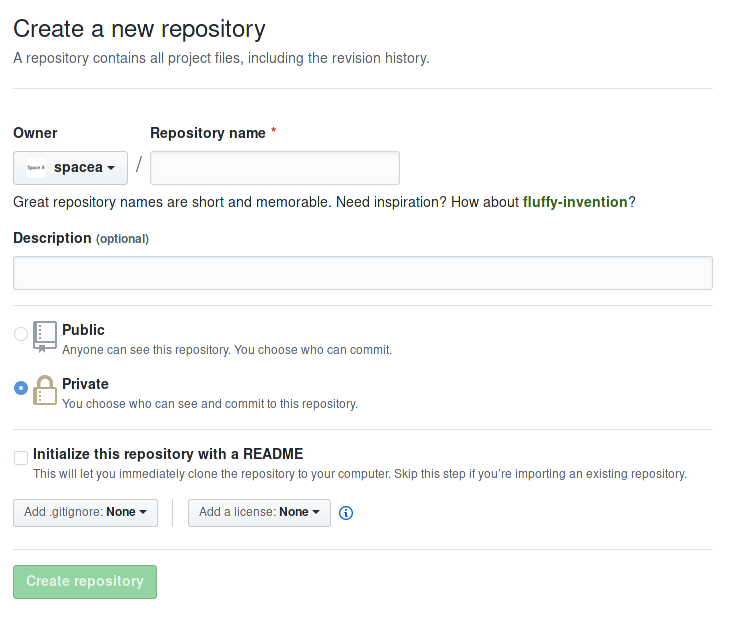
\includegraphics[width=0.8\linewidth]{images/gh-new-repo2} 

}

\caption{Okno tworzenia nowego repozytorium GitHub.}\label{fig:gh-new-repo2}
\end{figure}

Po wybraniu potwierdzenia (\emph{Create repository}) utworzone zostanie nowe, puste repozytorium (rycina \ref{fig:gh-new-repo3}).

\begin{figure}[H]

{\centering 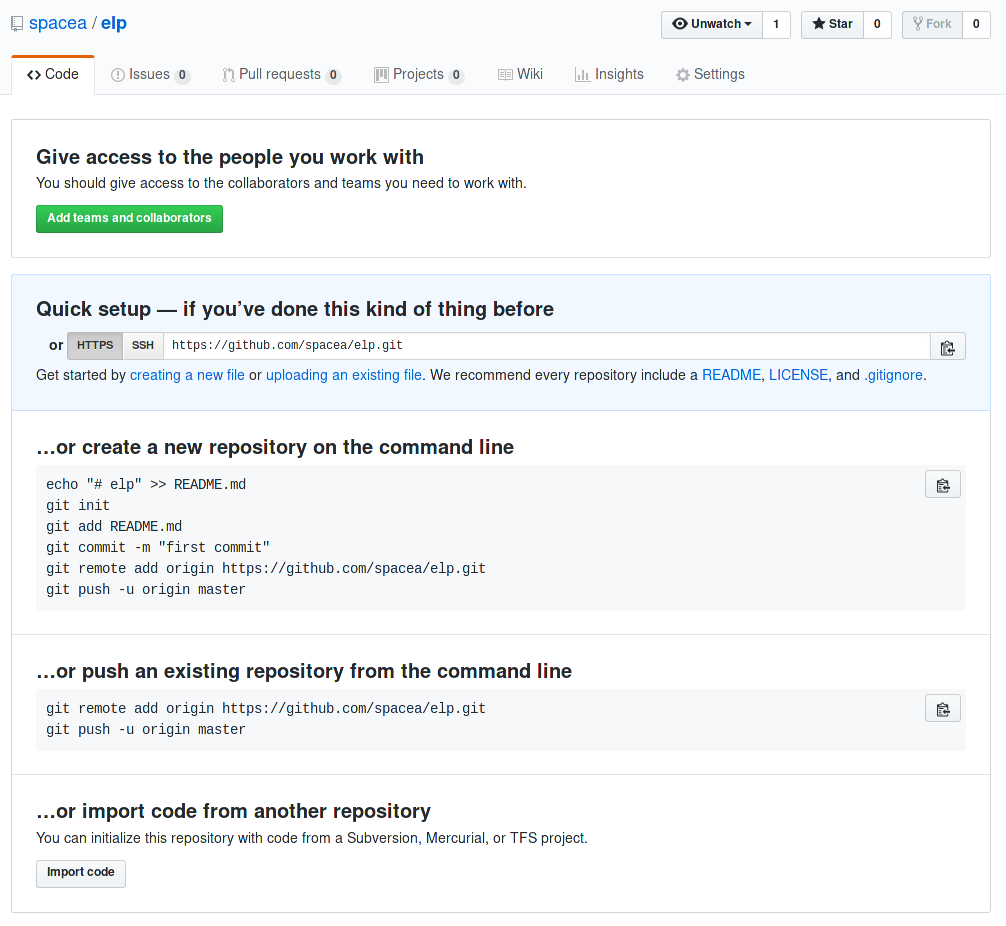
\includegraphics[width=0.8\linewidth]{images/gh-new-repo3} 

}

\caption{Nowe, puste repozytorium GitHub.}\label{fig:gh-new-repo3}
\end{figure}

Okno pustego repozytorium przedstawia cztery główne drogi pozwalające na dodanie zawartości:

\begin{enumerate}
\def\labelenumi{\arabic{enumi}.}
\tightlist
\item
  Szybka konfiguracja - tutaj podane są dwie możliwe ścieżki do zdalnego repozytorium.
  Pierwsza z nich to adres HTTPS a druga to adres SSH.
  W sekcji \ref{rstudio-git} zostanie wyjaśnione jak korzystać z szybkiej konfiguracji.
\item
  Stworzenie nowego repozytorium używając linii komend.
  Jest to używane w sytuacjach, gdy lokalna wersja repozytorium jeszcze nie istnieje.
  W tej sytuacji (1) tworzony jest nowy plik tekstowy \texttt{README.md}, (2) obecny katalog jest określany jako repozytorium Git, (3) plik \texttt{README.md} jest dodawany do repozytorium, (4) dodanie tego pliku jest zatwierdzone wraz z wiadomością ```first commit'', (5) dodana jest ścieżka do zdalnego repozytorium, (6) następuje wysłanie zmian z lokalnego do zdalnego repozytorium.
\item
  Wysłanie zmian z istniejącego repozytorium.
  Ta opcja przydaje się, gdy mamy już istniejące lokalne repozytorium, ale do którego nie ma jeszcze zdalnego repozytorium.
  Tutaj następuje tylko (1) dodanie ścieżki do zdalnego repozytorium oraz (2) wysłanie zmian z lokalnego do zdalnego repozytorium.
\item
  Import kodu z innego systemu kontroli wersji niż Git.
\end{enumerate}

\hypertarget{repozytorium-github}{%
\subsection{Repozytorium GitHub}\label{repozytorium-github}}

Wygląd okna repozytorium zmienia się po dodaniu pierwszej zawartości (rycina \ref{fig:gh-new-repo4}).

\begin{figure}[H]

{\centering 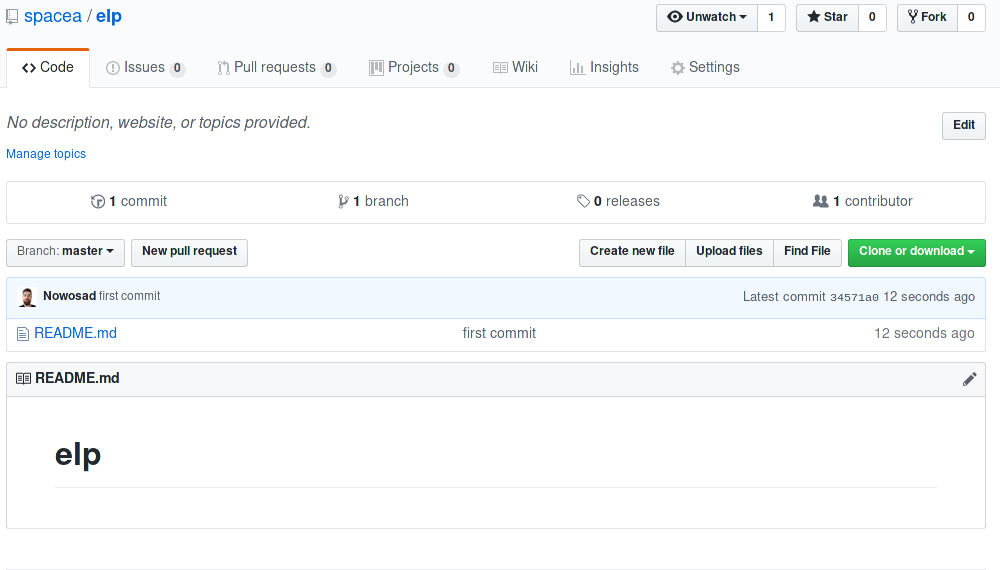
\includegraphics[width=0.8\linewidth]{images/gh-new-repo4} 

}

\caption{Repozytorium GitHub po dodaniu zawartości.}\label{fig:gh-new-repo4}
\end{figure}

Teraz możliwe jest podejrzenie występujących tam plików (w tym momencie jedynie plik \texttt{README.md}), zmian jakie zaszły w repozytorium (klikając na \emph{commit}), istniejących rozgałęzień (klikając na \emph{branch}) oraz wiele innych.
Pod zieloną ikoną \emph{Clone or download} można dodatkowo znaleźć ścieżkę do tego zdalnego repozytorium.

\hypertarget{dodatkowe-moux17cliwoux15bci-github}{%
\subsection{Dodatkowe możliwości GitHub}\label{dodatkowe-moux17cliwoux15bci-github}}

W prawym górnym rogu okna repozytorium (rycina \ref{fig:gh-new-repo4}) znajdują się trzy ikony - \emph{Watch}, \emph{Star}, \emph{Fork}.
Pierwsza z nich pozwala na określenie czy chcemy dostawać powiadomienia na temat dyskusji prowadzonych wewnątrz danego repozytorium, takich jak utworzenie nowej sprawy.
Druga ikona pozwala na oznaczanie interesujących repozytoriów i przez to ułatwiająca znajdowania podobnych projektów.
Ostatnia ikona \emph{Fork} oznacza w tym kontekście rozwidlenie.
Po jej kliknięciu następuje utworzenie kopii repozytorium innego użytkownika do naszego konta.

Oprócz dostępu do kodu i jego zmian, GitHub oferuje także szereg dodatkowych możliwości.
Obejmuje to, między innymi, automatyczne wyświetlanie plików README, śledzenie spraw (ang. \emph{issue tracking}), zapytania aktualizacyjne (ang. \emph{pull request}), wizualizacje zmian, czy nawet tworzenie stron internetowych.
Sprawy (ang. \emph{issues}) to miejsce, gdzie twórcy mogą zapisywać swoje listy zadań dotyczące danej aplikacji, a użytkownicy mogą zgłaszać błędy czy propozycje ulepszeń.
Zapytania aktualizacyjne są tworzone, np. w przypadku, gdy lokalnie zmieniliśmy zawartość repozytorium innego użytkownika\footnote{Może to być zarówno dodanie nowej możliwości, naprawienie błędu w kodzie, czy nawet poprawienie literówki w dokumentacji.} i chcemy zaproponować żeby nasza zmiana została dołączona do oryginalnego repozytorium.
W takiej sytuacji często opiera się~to o (1) stworzenie rozwidlenia (ang. \emph{fork}), (2) pobranie rozwidlenia jako lokalne repozytorium, (3) edycja lokalnego repozytorium, (4) zatwierdzenie zmian i wysłanie ich do zdalnego repozytorium (rozwidlenia), (5) zaproponowanie zapytania aktualizacyjnego.

Możliwe jest również łączenie możliwości serwisu GitHub z innymi serwisami internetowymi, takimi jak \href{https://travis-ci.org/}{Travis CI}, \href{https://codecov.io/}{Codecov}, \href{https://gitter.im/}{Gitter} i \href{https://github.com/marketplace}{wiele innych}.

\hypertarget{rstudio-git}{%
\section{Kontrola wersji w RStudio}\label{rstudio-git}}

RStudio posiada wbudowane, uproszczone graficzne wsparcie dla systemu Git.
Istnieje też szereg programów, których głównym celem jest ułatwienie pracy z systemem Git.
Nazwane są one klientami Git, wśród których można wymienić \href{https://www.gitkraken.com/}{GitKraken} i \href{https://www.sourcetreeapp.com/}{Sourcetree}.

Najprostszym sposobem połączenia RStudio z systemem Git i serwisem GitHub jest stworzenie nowego projektu:

\begin{enumerate}
\def\labelenumi{\arabic{enumi}.}
\tightlist
\item
  Kliknąć \texttt{File\ -\textgreater{}\ New\ Project}.
\item
  Wybrać \texttt{Version\ Control}.
\item
  Wybrać \texttt{Git}.
\item
  Podać ścieżkę do zdalnego repozytorium (adres HTTPS lub SSH) oraz wybrać miejsce na dysku, gdzie ma się~ten projekt znajdować.
\item
  Kliknąć \texttt{Create\ Project}.
\end{enumerate}

W efekcie zostanie utworzony nowy projekt RStudio (w tle wykonywane jest pobranie kopii istniejącego zdalnego repo - patrz sekcja \ref{repozytorium-zdalne}), który jednocześnie jest lokalnym repozytorium Git.
Dodatkowo, w RStudio pojawi się~nowy panel ``Git'' (rycina \ref{fig:rstudio-git}).

\begin{figure}[H]

{\centering 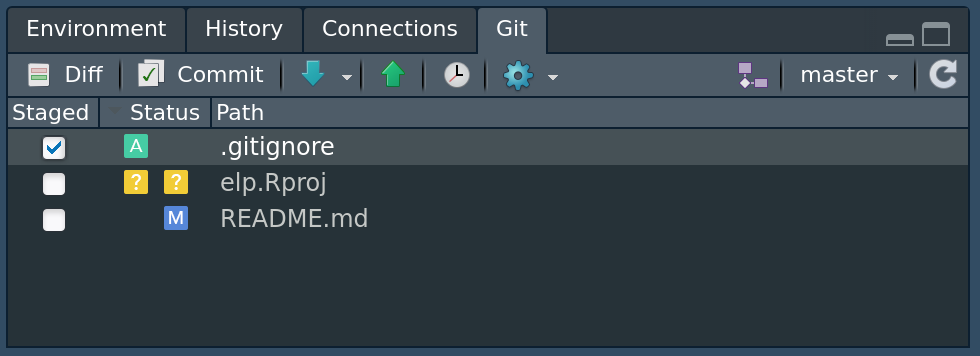
\includegraphics[width=0.8\linewidth]{images/rstudio-git} 

}

\caption{Panel Git w RStudio.}\label{fig:rstudio-git}
\end{figure}

W tym panelu są wyświetlone (1) wszystkie pliki, które są w folderze projektu, ale nie w repozytorium Git (żółte ikony statusu), (2) pliki, które chcemy dodać do repozytorium (zielona ikona statusu), oraz (3) pliki, które są już w repozytorium, ale zostały zmodyfikowane (niebieska ikona statusu).\footnote{Możliwe są też~inne sytuacje, np. czerwona ikona z literą R sugerująca zmianę nazwy pliku.}
Ten panel nie pokazuje plików, które nie zostały ostatnio zmienione.
Pierwsza kolumna w tym panelu (\emph{Staged}) domyślnie zawiera same nieodhaczone białe pola.
Wybór tego pola (jego odhaczenie) jest równoznaczne z dodaniem zmian (więcej informacji można znaleźć w sekcji \ref{dodawanie-zmian}).

Dodatkowo nad listą plików znajduje się szereg ikon.
Pierwsze dwie z nich (\emph{Diff} i \emph{Commit}) wyświetlają okno, które pozwala sprawdzić jakie zmiany zaszły w plikach od ostatniego ich dodania (dolny panel; sekcja \ref{sprawdzanie-zmian}) oraz zatwierdzić zmiany (prawy panel; sekcja \ref{zatwierdzanie-zmian}).
Kolejne, strzałki w dół i górę, oznaczają odpowiednio aktualizowanie zmian (sekcja \ref{aktualizowanie-zmian}) i wysyłanie zmian (sekcja \ref{wysylanie-zmian}).
Ikona zegarka otwiera nowe okno, w którym można zobaczyć jakie zmiany zaszły w kolejnych zatwierdzeniach zmian (tak zwanych \emph{commitach}).
Następne ikony pozwalają na określenie plików do ignorowania (ikona koła zębatego) oraz tworzenie nowych rozgałęzień.
Przedostatni element tego okna to nazwa obecnie ustawionego rozgałęzienia, a po kliknięciu tej nazwy możliwa jest przejście do innego rozgałęzienia (sekcja \ref{branches}).

\hypertarget{sposoby-pracy-z-systemem-git}{%
\section{Sposoby pracy z systemem Git}\label{sposoby-pracy-z-systemem-git}}

Istnieje wiele możliwych sposobów pracy z systemem Git.
Zależą one od wielu czynników, takich jak planowany cel repozytorium czy wykorzystywana technologia.
Dodatkowo znaczny wpływ na sposób pracy z systemem Git ma czynnik ludzki - przyzwyczajenia osób pracujących nad projektem i ich preferencje.

\hypertarget{nowy-projekt}{%
\subsection{Nowy projekt}\label{nowy-projekt}}

Preferowanym sposobem rozpoczęcia pracy nad nowym zadaniem (projektem) w R jest stworzenie nowego, pustego repozytorium w serwisie GitHub, a następnie połączenie z nim nowego projektu RStudio.
Taki sposób został opisany na początku sekcji \ref{rstudio-git}.

W momencie, gdy posiadamy ustawione zarówno lokalne jak i zdalne repozytorium możliwe jest rozpoczęcie pracy.
Teraz można tworzyć nowe oraz edytować istniejące pliki.
Po każdej wyraźnej zmianie plików (np. ulepszenie kodu, naprawa błędów, dodanie nowych możliwości) należy dodać zmiany oraz je zatwierdzić.
Można to zrobić klikając pole \emph{Staged} przy wybranych plikach oraz następnie ikonę \emph{Commit}.
Teraz można dodać wiadomość opisująca zmiany jakie zaszły, oraz ją zatwierdzić klikając przycisk \emph{Commit}.
Zalecane jest, aby powyższą czynność wykonywać nawet wiele razy dziennie.

\begin{rmdinfo}
Często w folderze projektu możesz posiadać pliki, których nie chcesz dodawać do repozytorium.
W takiej sytuacji dodaj ich nazwy do pliku \texttt{.gitignore} i staną się one niewidoczne dla systemu Git.
\end{rmdinfo}

Efektem powyższej operacji jest posiadanie zatwierdzonych zmian w lokalnym repozytorium, ale jeszcze ich brak w repozytorium zdalnym.
Kolejnym krokiem jest przesłanie zmian na zdalne repozytorium.
Tutaj zalecane jest najpierw kliknięcie ikony aktualizowania zmian (strzałka w dół), aby upewnić się, że posiadamy aktualną wersję repozytorium, a następnie kliknięcie ikony wysyłania zmian (strzałka w górę).
Jeżeli wszystko poszło zgodnie z planem, nowa wersja repozytorium powinna pojawić się na odpowiedniej stronie serwisu GitHub.
Tą czynność warto wykonywać rzadziej niż poprzednią, ale też regularnie.

Dalej praca polega na powtarzaniu tych czynności:

\begin{enumerate}
\def\labelenumi{\arabic{enumi}.}
\tightlist
\item
  Edycja/dodanie plików czy folderów.
\item
  Dodanie zmian.
\item
  Zatwierdzenie zmian.
\item
  Sprawdzenie czy posiadamy aktualną wersję repozytorium.
\item
  Wysyłania zmian na zdalne repozytorium.
\end{enumerate}

\hypertarget{istniejacy-projekt}{%
\subsection{Istniejący projekt}\label{istniejacy-projekt}}

Czasami posiadasz już~jakiś istniejący projekt, ale chcesz do niego dodać możliwości kontroli wersji.
W takich przypadkach najprostszy sposób to stworzenie nowego repozytorium w serwisie GitHub oraz pustego, połączonego z nim nowego projektu RStudio.
Następnie należy przekopiować do tego projektu wszystkie już istniejące pliki, dodać je (pole \emph{Staged}), zatwierdzić oraz przesłać na zdalne repozytorium.

Kolejne etapy pracy wyglądają identycznie jak w poprzedniej sekcji.

\hypertarget{problemy-z-kontrolux105-wersji}{%
\section{Problemy z kontrolą wersji}\label{problemy-z-kontrolux105-wersji}}

W ramach jednego projektu często posiadamy wiele plików z długą historią zmian, do tego nanoszonych przez szereg różnych osób.
Jest to sytuacja w której dość prosto o wystąpienie problemów czy nieoczekiwanych (przez użytkownika) zachowań systemu kontroli wersji Git.

Jednym z najczęstszych problemów jest pojawienie się poniższego komunikatu podczas próby wysyłania zmian do zdalnego repozytorium.

\begin{Shaded}
\begin{Highlighting}[]
\OperatorTok{>>>} \FunctionTok{git}\NormalTok{ push}
\ExtensionTok{To}\NormalTok{ https://github.com/YOU/REPO.git}
\NormalTok{ ! [}\ExtensionTok{rejected}\NormalTok{]        master -}\OperatorTok{>}\NormalTok{ master (fetch first)}
\ExtensionTok{error}\NormalTok{: failed to push some refs to }\StringTok{'https://github.com/YOU/REPO.git'}
\ExtensionTok{hint}\NormalTok{: Updates were rejected because the remote contains work that you do}
\ExtensionTok{hint}\NormalTok{: not have locally. This is usually caused by another repository pushing}
\ExtensionTok{hint}\NormalTok{: to the same ref. You may want to first integrate the remote changes}
\ExtensionTok{hint}\NormalTok{: (e.g., }\StringTok{'git pull ...'}\NormalTok{) }\ExtensionTok{before}\NormalTok{ pushing again.}
\ExtensionTok{hint}\NormalTok{: See the }\StringTok{'Note about fast-forwards'}\NormalTok{ in }\StringTok{'git push --help'}\NormalTok{ for details.}
\end{Highlighting}
\end{Shaded}

Oznacza on, że w repozytorium zdalnym są jakieś zmiany, których nie ma lokalnie.
Prawdopodobnie wynikają one z kwestii, że inna osoba przesłała swoje zmiany do zdalnego repozytorium lub też pliki były zmienione i przesłane przez ciebie na innym komputerze.
Najczęściej w takiej sytuacji wystarczy aktualizowanie zmian ze zdalnego repo (ikona strzałki w dół), a następnie ponowienie próby wysłania zmian.
Czasem jednak mogły zajść zmiany w tym samym pliku edytowanym przez wiele osób.
Wówczas konieczne jest ręczne poprawienie problematycznych plików, dodanie zmian i ich zatwierdzenie.

Z racji popularności systemu Git istnieje ogromna liczba materiałów pomagających w jego nauce i zrozumieniu oraz wiele stron zawierających pytania i odpowiedzi dotyczące napotkanych problemów.
W przypadku łączenia możliwości języka R z systemem Git warto poczytać materiały zawarte na stronie \url{https://happygitwithr.com/} \citep{bryanHappyGitGitHub2019} oraz rozdział \href{https://r-pkgs.org/git.html}{Git and GitHub} książki R packages \citep{wickham2015r}.
Do ogólnego wprowadzenia do systemu Git może posłużyć darmowa książka online \href{https://git-scm.com/book/pl/v2}{Pro Git} \citep{chacon2014pro}, której kilka pierwszych rozdziałów jest również dostępna w języku polskim.
Git jest również bardzo popularnym tematem na serwisie stackoverflow, gdzie można znaleźć~\href{https://stackoverflow.com/questions/tagged/git}{pytania i odpowiedzi na różnorodne tematy z nim związane}.
Więcej odnośników do materiałów związanych z sytemem Git i serwisem GitHub można znaleźć na stronach \href{https://help.github.com/en/articles/git-and-github-learning-resources}{pomocy GitHub}.

\hypertarget{zadania}{%
\section{Zadania}\label{zadania}}

\begin{enumerate}
\def\labelenumi{\arabic{enumi})}
\tightlist
\item
  Skonfiguruj system Git podając swoją nazwę użytkownika oraz adres email.
  Sprawdź czy nazwa została dodana używając komendy \texttt{git\ config\ -\/-global\ user.name} oraz czy dodany został adres email używając \texttt{git\ config\ -\/-global\ user.email}.
\item
  Stwórz nowe konto użytkownika lub zaloguj się na swoje istniejące konto GitHub.
  Utwórz nowe publiczne repozytorium o nazwie ``test''.
\item
  Połącz zdalne repozytorium ``test'' z nowym projektem RStudio.
  Sprawdź czy w RStudio pojawił się panel Git, a następnie w tym panelu dodaj pliki \texttt{.gitignore} i \texttt{test.Rproj} do repozytorium Git poprzez odhaczenie odpowiednich pól w kolumnie \emph{Staged}.
  Kliknij ikonę \emph{Commit} i wpisz wiadomość ``Dodano pliki .gitignore i test.Rproj'' w pole po prawej stronie.
  Zatwierdź tą wiadomość, a następnie prześlij te zmiany do repozytorium zdalnego.
\item
  Sprawdź stronę internetową zawierającą zdalne repozytorium ``test''.
  Czy zaszły na niej jakieś zmiany od poprzedniego wejścia?
  Przejrzyj jakie dodatkowe opcje pojawiły się na stronie tego repozytorium.
\item
  W projekcie ``test'' w RStudio stwórz nowy plik \texttt{README.md}.
  Do tego pliku wstaw zdanie poniższy tekst:
\end{enumerate}

\begin{verbatim}
# test

To jest moje pierwsze repozytorium!
\end{verbatim}

Dodaj ten plik do repozytorium Git, napisz odpowiedni komunikat, zatwierdź zmiany i prześlij je do repozytorium zdalnego.
Sprawdź stronę internetową zawierającą zdalne repozytorium ``test''.
Czy zaszły na niej jakieś zmiany od poprzedniego wejścia?

\begin{enumerate}
\def\labelenumi{\arabic{enumi})}
\setcounter{enumi}{5}
\item
  Z poziomu strony internetowej swojego repozytorium ``test'' edytuj plik \texttt{README.md}.
  Możesz to zrobić klikając na nazwę tego pliku, a następnie na ikonę ołówka w prawym górnym roku okna.
  Dodaj do niego kolejną linię \texttt{Edytowałem\ plik\ z\ poziomu\ GitHub.} oraz napisz odpowiedni komunikat poniżej tego okna i zatwierdź zmiany (zielony przycisk \texttt{Commit\ changes}).
  Sprawdź stronę internetową zawierającą zdalne repozytorium ``test''.
  Czy zaszły na niej jakieś zmiany od poprzedniego wejścia?
\item
  Wróć do swojego projektu RStudio.
  Zobacz jak wygląda lokalny plik \texttt{README.md} - powinien on nadal zawierać wcześniej wprowadzony tekst.
\end{enumerate}

\begin{verbatim}
# test

To jest moje pierwsze repozytorium!
\end{verbatim}

Kliknij w ikonę aktualizowania zmian (strzałka w dół).
Zobacz jak teraz wygląda lokalny plik \texttt{README.md}.
Co się w nim zmieniło?

\hypertarget{tworzenie-pakietow}{%
\chapter{Pakiety}\label{tworzenie-pakietow}}

Pakiety są powszechnie wykorzystywane podczas pracy z językiem R.
Celem sekcji \ref{pakiety} było wprowadzenie do tego czym one są, jak się je instaluje oraz dołącza.
Najważniejszą tam informacją było, że pakiety są zorganizowanymi zbiorami funkcji.
Oznacza to, że nie tylko posiadamy pewną liczbę stworzonych funkcji, ale także są one ułożone w pewien ustalony sposób.
Funkcje w pakietach posiadają też swoją dokumentację (jej struktura została przedstawiona w sekcji \ref{dokumentacja-funkcji}) czy przykładowe dane.
Pakiety, oprócz swojej unikalnej nazwy, posiadają również informacje o swojej wersji, autorach, zależnościach i licencji.

Informacje w tym rozdziale powinny pozwolić na stworzenie podstawowego pakietu R.
Istnieje jednak wiele dodatkowych aspektów i kwestii w tym temacie, które zostały tutaj wspomniane pobieżnie lub pominięte.
W celu poznania i zrozumienia złożonych aspektów tworzenia pakietów R cennymi źródłami wiedzy może być książki \href{https://r-pkgs.org}{R packages} \citep{wickham2015r} oraz \href{https://ropensci.github.io/dev_guide/}{rOpenSci Packages: Development, Maintenance, and Peer Review} \citep{ropensci_2019_2554759}.
Dodatkowo, w niektórych przypadkach pomocna może być oficjalna dokumentacja \href{https://cran.r-project.org/doc/manuals/R-exts.html\#Creating-R-packages}{Writing R Extensions} \citep{team1999writing}.

\hypertarget{nazwa-pakietu}{%
\section{Nazwa pakietu}\label{nazwa-pakietu}}

Nazwa nowego pakietu musi spełniać kilka wymagań: składać się tylko ze znaków \href{https://en.wikipedia.org/wiki/ASCII}{ASCII}, cyfr i kropek, mieć co najmniej dwa znaki oraz zaczynać się od litery i nie kończyć się kropką \citep{team1999writing}.
Ważne jest również myślenie o nazwie pakietu tak jak o nazwach funkcji (sekcja \ref{styl}) - nazwy pakietów powinny ułatwiać zrozumienie ich zawartości.
Dodatkowo, z uwagi na istnienie wielu pakietów warto najpierw sprawdzić czy pakiet o wymyślonej przez nas nazwie już nie istnieje.
Można to przykładowo zrobić używając pakietu \textbf{available} \citep{R-available}, który sprawdza przy wybrana nazwa nie jest już zajęta oraz czy nie ma ona jakiegoś niepożądanego przez nas znaczenia.

\hypertarget{tworzenie-szkieletu-pakietu}{%
\section{Tworzenie szkieletu pakietu}\label{tworzenie-szkieletu-pakietu}}

Kolejnym krokiem jest stworzenie szkieletu pakietu, czyli zorganizowanego zbioru plików i folderów, do których później należy dodać odpowiednie informacje i funkcje.
Znacznie w tym może pomóc pakiet \textbf{usethis} \citep{R-usethis}, który zawiera szereg funkcji ułatwiających budowanie pakietów R.

\begin{Shaded}
\begin{Highlighting}[]
\KeywordTok{library}\NormalTok{(usethis)}
\end{Highlighting}
\end{Shaded}

Do stworzenia szkieletu pakietu służy funkcja \texttt{create\_packages()}, w której należy podać ścieżkę do nowego pakietu.
W tej ścieżce ostatnia nazwa folderu określa również nazwę pakietu.\footnote{Funkcja również \texttt{create\_packages()} sama tworzy nowy folder, jeżeli on wcześniej nie istniał.}

\begin{Shaded}
\begin{Highlighting}[]
\NormalTok{usethis}\OperatorTok{::}\KeywordTok{create_package}\NormalTok{(}\StringTok{"~/Documents/mojpakiet"}\NormalTok{)}
\end{Highlighting}
\end{Shaded}

W efekcie działania powyższej funkcji stworzony zostanie nowy folder \texttt{mojpakiet} zawierający kilka plików oraz otwarty zostanie nowy projekt RStudio zawierający ten pakiet.
Najważniejsze nowe pliki to:

\begin{enumerate}
\def\labelenumi{\arabic{enumi}.}
\tightlist
\item
  \texttt{mojpakiet.Rproj} - plik projektu RStudio
\item
  \texttt{DESCRIPTION} - plik zawierający podstawowe informacje o pakiecie
\item
  \texttt{R/} - w tym pustym folderze konieczne będzie umieszczenie nowych funkcji R
\item
  \texttt{NAMESPACE} - ten plik określa, między innymi, jakie funkcje są dostępne w tym pakiecie.
  Ten plik i jego zawartość jest tworzona automatycznie
\end{enumerate}

Dodatkowo w prawym górnym panelu RStudio pojawi się nowy panel ``Build''.

\hypertarget{opis-pakietu}{%
\section{Opis pakietu}\label{opis-pakietu}}

Plik \texttt{DESCRIPTION} zawiera opis (metadane) pakietu, w tym jego nazwę, tytuł, wersję, autorów, opis, czy licencję.

\begin{Shaded}
\begin{Highlighting}[]
\FunctionTok{Package:}\AttributeTok{ mojpakiet}
\FunctionTok{Title:}\AttributeTok{ Moje Funkcje Robiace Wszystko}
\FunctionTok{Version:}\AttributeTok{ 0.0.1}
\FunctionTok{Authors@R:}\AttributeTok{ }
\NormalTok{    person(given = }\StringTok{"Imie"}\NormalTok{,}
\NormalTok{           family = }\StringTok{"Nazwisko"}\NormalTok{,}
\NormalTok{           role = c(}\StringTok{"cre"}\NormalTok{, }\StringTok{"aut"}\NormalTok{),}
\NormalTok{           email = }\StringTok{"imie.nazwisko@example.com"}\NormalTok{)}
\FunctionTok{Description:}\AttributeTok{ Tworzenie, przeliczanie i wyliczanie wszystkiego. }
\NormalTok{    Czasami nawet więcej.}
\FunctionTok{License:}\AttributeTok{ CC0}
\FunctionTok{Encoding:}\AttributeTok{ UTF-8}
\FunctionTok{LazyData:}\AttributeTok{ true}
\FunctionTok{RoxygenNote:}\AttributeTok{ 6.1.1}
\end{Highlighting}
\end{Shaded}

Tytuł pakietu (\texttt{Title:}) w jednym krótkim zdaniu (sloganie) określa do czego służy ten pakiet.\footnote{Tytuły pakietów można znaleźć, np. w panelu ``Packages'' w RStudio.}
Składa się on ze słów rozpoczynających się z dużej litery.

Wersja pakietu (\texttt{Version:}) pozwala jego użytkownikom na zobaczenie, czy korzystają z aktualnej wersji pakietu.
Zalecanym sposobem określania wersji pakietu jest stosowanie trzech liczb \texttt{pierwsza.druga.trzecia}, np. \texttt{0.9.1}.
Zmiana trzeciej liczby służy do pokazania, że zaszła niewielka zmiana w kodzie, zazwyczaj wiążąca się z naprawą małego błędu, np. \texttt{0.9.2}.
Druga liczba jest zmieniana podczas wydania nowej wersji pakietu, która zawiera większe zmiany w kodzie, jak naprawy poważnych błędów, czy dodanie nowych możliwości, np. \texttt{0.10.0}.
Zmiana pierwszej liczby sugeruje poważne zmiany w kodzie, które ale też sugeruje pewną stabilizację działania, np. \texttt{1.0.0}.

\texttt{Authors@R:} określa kolejne osoby zaangażowane w budowę tego pakietu.
W powyższym przykładzie mamy wymienioną jedną osobę \texttt{"Imie"} \texttt{"Nazwisko"}, której adres mailowy to \texttt{"imie.nazwisko@example.com"}.
Dodatkowo ta osoba posiada dwie role przy tworzeniu tego pakietu \texttt{"cre"} oraz \texttt{"aut"}.
Pierwsza rola, \texttt{"cre"}, informuje że ta osoba jest twórcą i konserwatorem tego pakietu.
Ona jest odpowiedzialna za pracę pakietu.
Druga rola, \texttt{"aut"}, jest nadawana osom, które wniosły bardzo duży wkład w kod zawarty w pakiecie.
Inne często używane role to \texttt{"ctb"} określająca osoby, które wniosły mniejszy wkład w kod (np. drobne zmiany) oraz \texttt{"cph"} określająca osoby czy instytucje będące posiadaczami praw autorskich (np. firma zatrudniająca autora kodu albo autor biblioteki, która została wewnętrznie użyta).\footnote{Pełną listę dostępnych ról można znaleźć pod adresem \url{http://www.loc.gov/marc/relators/relaterm.html}.}
Dodanie kolejnych osób odbywa się poprzez łączenie ich funkcją \texttt{c()}.

\begin{Shaded}
\begin{Highlighting}[]
\FunctionTok{Authors@R:}\AttributeTok{ c(}
\NormalTok{    person(}\StringTok{"Imie"}\NormalTok{, }\StringTok{"Nazwisko"}\NormalTok{, role = c(}\StringTok{"cre"}\NormalTok{, }\StringTok{"aut"}\NormalTok{), email = }\StringTok{"email1@example.com"}\NormalTok{),}
\NormalTok{    person(}\StringTok{"Imie2"}\NormalTok{, }\StringTok{"Nazwisko2"}\NormalTok{, role = }\StringTok{"aut"}\NormalTok{, email = }\StringTok{"email2@example.com"}\NormalTok{)}
\NormalTok{)}
\end{Highlighting}
\end{Shaded}

Licencja (\texttt{License:}) określa warunki korzystania z pakietu przez inne osoby.
W bardzo dużym skrócie licencje oprogramowania można podzielić na licencje otwarte (\emph{open-source}) oraz zamknięte (\emph{proprietary}).
Najpopularniejsze licencje otwarte używane w pakietach R to licencja \texttt{CC0}, \texttt{MIT} oraz \texttt{GPL}.
Pierwsza z nich, \texttt{CC0} oznacza przekazanie \href{https://creativecommons.org/publicdomain/zero/1.0/deed.pl}{zawartości pakietu do domeny publicznej} i najczęściej stosowana jest do pakietów zawierających tylko zbiory danych.
Licencja \texttt{MIT} daje nieograniczone prawo do używania, modyfikowania i rozpowszechniania kodu, pod warunkiem zachowania informacji o autorze.
Dodanie licencji \texttt{MIT} do pakietu R można wykonać podając swoje imię i nazwisko w funkcji \texttt{usethis::use\_mit\_license("Imie\ Nazwisko")}.
W ten sposób informacja o tej licencji zostanie dodana do pliku \texttt{DESCRIPTION} (\texttt{License:\ MIT\ +\ file\ LICENSE}) oraz zostaną utworzone specjalne pliki z treścią licencji.
Trzecia z licencji otwartych, \texttt{GPL} (ang. \emph{GNU General Public License}) pozwala użytkownikom na uruchamianie, dostosowywanie, rozpowszechnianie i udoskonalanie kodu.
Ważną cechą tej licencji jest wymaganie, że wszelkie prace oparte o kod w licencji \texttt{GPL} również muszą mieć licencję \texttt{GPL}
Oprogramowanie zamknięte może również przyjmować wiele form (np. freeware czy też oprogramowanie komercyjne).
Określenie pakietu jako oprogramowania zamkniętego odbywa się poprzez dodanie informacji, że licencja znajduje się w pliku \texttt{LICENSE} (\texttt{License:\ file\ LICENSE}), a następnie stworzenie pliku tekstowego o tej nazwie zawierającego odpowiednią modyfikację poniższego tekstu:

\begin{Shaded}
\begin{Highlighting}[]
\NormalTok{Proprietary }

\NormalTok{Do not distribute outside of NAZWA MOJEJ FIRMY.}
\end{Highlighting}
\end{Shaded}

Plik \texttt{DESCRIPTION} należy regularnie uaktualniać, np. zmieniać numer wersji po naniesionych zmianach w kodzie, czy dodawać nowych autorów, jeżeli tacy się pojawili.

\hypertarget{rozwijanie-pakietu}{%
\section{Rozwijanie pakietu}\label{rozwijanie-pakietu}}

Rozwój pakietu R może opierać się na kilku poniższych krokach:

\begin{enumerate}
\def\labelenumi{\arabic{enumi}.}
\tightlist
\item
  Tworzenie/modyfikowanie kodu
\item
  Używanie funkcji \texttt{devtools::load\_all()}, która dodaje nowe/zmodyfikowane funkcje do R
\item
  Sprawdzenie czy funkcja działa zgodnie z oczekiwaniami na kilku przykładach
\item
  Dodanie testów jednostkowych (sekcja \ref{wbudowane-testy}) na podstawie stworzonych przykładów
\item
  Uaktualnienie dokumentacji tworzonego/modyfkowanego kodu
\item
  Wygenerowanie plików z dokumentacją używając \texttt{devtools::document()}
\item
  Sprawdzenie czy pakiet nie posiada żadnych problemów używając \texttt{devtools::check()}
\item
  Modyfikacja wersji oprogramowania w pliku \texttt{DESCRIPTION}
\item
  Powtórzenie powyższych czynności
\end{enumerate}

\hypertarget{tworzenie-i-dokumentacja-funkcji}{%
\section{Tworzenie i dokumentacja funkcji}\label{tworzenie-i-dokumentacja-funkcji}}

W sekcji \ref{budowanie-funkcji} stworzyliśmy nową funkcję \texttt{konwersja\_temp()} przeliczającą temperaturę ze stopni Fahrenheita na stopnie Celsjusza.

\begin{Shaded}
\begin{Highlighting}[]
\NormalTok{konwersja_temp =}\StringTok{ }\ControlFlowTok{function}\NormalTok{(temperatura_f)\{}
\NormalTok{    (temperatura_f }\OperatorTok{-}\StringTok{ }\DecValTok{32}\NormalTok{) }\OperatorTok{/}\StringTok{ }\FloatTok{1.8}
\NormalTok{\}}
\end{Highlighting}
\end{Shaded}

Umieszczenie tej funkcji w nowym pakiecie R odbywa się poprzez zapisanie tego kodu jako skrypt R (np. \texttt{konwersja\_temp.R}) w folderze \texttt{R/}.

Funkcje zawarte w pakietach muszą także posiadać odpowiednią dokumentację, zawierającą, między innymi, tytuł funkcji, opis jej działania, wyjaśnienie kolejnych argumentów funkcji, oraz przykłady jej działania.
Linie obejmujące dokumentację funkcji rozpoczynają się od znaków \texttt{\#\textquotesingle{}}, a tworzenie dokumentacji funkcji odbywa się poprzez wypełnianie treści dla kolejnych znaczników (np. \texttt{@example} określa występowanie przykładu).

Przykładowy plik \texttt{R/konwersja\_temp.R} może wyglądać następująco:

\begin{Shaded}
\begin{Highlighting}[]
\CommentTok{#' Konwersja temperatur}
\CommentTok{#'}
\CommentTok{#' @description Funkcja sluzaca do konwersji temperatury }
\CommentTok{#'   ze stopni Fahrenheita do stopni Celsjusza.}
\CommentTok{#'}
\CommentTok{#' @param temperatura_f wektor zawierajacy wartosci temperatury }
\CommentTok{#'   w stopniach Fahrenheita}
\CommentTok{#'}
\CommentTok{#' @return wektor numeryczny}
\CommentTok{#' @export}
\CommentTok{#'}
\CommentTok{#' @examples}
\CommentTok{#' konwersja_temp(75)}
\CommentTok{#' konwersja_temp(110)}
\CommentTok{#' konwersja_temp(0)}
\CommentTok{#' konwersja_temp(c(0, 75, 110))}
\NormalTok{konwersja_temp =}\StringTok{ }\ControlFlowTok{function}\NormalTok{(temperatura_f)\{}
\NormalTok{  (temperatura_f }\OperatorTok{-}\StringTok{ }\DecValTok{32}\NormalTok{) }\OperatorTok{/}\StringTok{ }\FloatTok{1.8}
\NormalTok{\}}
\end{Highlighting}
\end{Shaded}

Pierwsza linia w tym pliku określa tytuł danej funkcji.
Kolejny element rozpoczynający się od znacznika \texttt{@description} zawiera krótki opis tego, co funkcja robi.
Następnie zazwyczaj wypisane są wszystkie argumenty danej funkcji używając kolejnych znaczników \texttt{@param}.
Znacznik \texttt{@return} pozwala na przekazanie informacji o tym co jest zwracane jako efekt działania funkcji.
Przedostatnim znacznikiem w powyższym przypadku jest \texttt{@export}.
Oznacza on, że ta funkcja będzie widoczna dla każdego użytkownika tego pakietu po użyciu \texttt{library(mojpakiet)}.
Bez tego znacznika funkcja byłaby tylko widoczna wewnątrz pakietu.
Ostatni znacznik, \texttt{@examples}, wypisuje kolejne przykłady działania funkcji.

Wybór \texttt{More\ -\textgreater{}\ Document} w panelu ``Build'' (inaczej wywołanie funkcji \texttt{devtools::document()} lub użycie skrótu CTRL+SHIFT+D) spowoduje zbudowanie pliku dokumentacji w folderze \texttt{man}, np. \texttt{man/konwersja\_temp.Rd}.
Pliki dokumentacji będą zawsze tworzone w ten sposób - nie należy ich modyfikować ręcznie.
Zbudowanie pliku dokumentacji pozwala teraz na jej podejrzenie poprzez wywołanie pliku pomocy naszej funkcji:

\begin{Shaded}
\begin{Highlighting}[]
\NormalTok{?konwersja_temp}
\end{Highlighting}
\end{Shaded}

\hypertarget{zaleux17cnoux15bci}{%
\section{Zależności}\label{zaleux17cnoux15bci}}

Istnieje jedna ważna różnica pomiędzy tworzeniem funkcji w skryptach a tworzeniem jej wewnątrz pakietu - w pakietach nie można używać dołączania pakietów za pomocą funkcji \texttt{library()}.
Zamiast tego możliwe jest definiowanie każdej zewnętrznej funkcji używając operatora \texttt{::}.\footnote{Istnieją również inne możliwości, np. użycie znaczników \texttt{@import} lub \texttt{@importFrom}.}

Dodatkowo każda zależność z zewnętrznym pakietem musi być określona w pliku \texttt{DESCRIPTION}.
Jest to możliwe używając wpisów \texttt{Imports:} oraz \texttt{Suggests:}, przykładowo:\footnote{Istnieją również inne wpisy, takie jak \texttt{Depends:}, \texttt{LinkingTo:}, czy \texttt{Enhances:}.}

\begin{Shaded}
\begin{Highlighting}[]
\FunctionTok{Imports:}
\NormalTok{  stringr,}
\NormalTok{  readr}
\FunctionTok{Suggests:}
\NormalTok{  readxl}
\end{Highlighting}
\end{Shaded}

\texttt{Imports:} określa pakiety, które muszą być zainstalowane, aby tworzony pakiet mógł zadziałać.
Jeżeli wymienione tutaj pakiety nie będą znajdować się na komputerze użytkownika to zostaną one automatycznie doinstalowane podczas instalacji naszego pakietu.
\texttt{Suggests:} wymienia pakiety, które pomagają w użytkowaniu naszego pakietu, np. takie które zawierają testowe dane.
Wymienione tutaj pakiety nie będą automatycznie doinstalowane podczas instalacji naszego pakietu.

\hypertarget{sprawdzanie-pakietu}{%
\section{Sprawdzanie pakietu}\label{sprawdzanie-pakietu}}

W momencie, gdy pakiet posiada już swoje podstawowe elementy, tj. pierwsze udokumentowane funkcje oraz uzupełniony opis wraz z zależnościami warto sprawdzić czy te wszystkie elementy pakietu dobrze współgrają ze sobą.
Można to zrobić używając funkcji \texttt{devtools::check()} (inaczej wybór \texttt{Check} w panelu ``Build'' RStudio lub skrót CTRL+SHIFT+E).
W efekcie tego wywołania zostanie uruchomiony szereg sprawdzeń i testów dotyczących pakietu, jego funkcji czy opisu.
Na końcu zwrócone zostanie wypisanie liczby błędów (\emph{error}), ostrzeżeń (\emph{warnings}) i notatek (\emph{notes}), poprzedzone wymienieniem każdego ich wystąpienia.
Błędy oznaczają, że z jakiegoś powodu pakietu nie można zbudować, ostrzeżenia natomiast sugerują sytuację w której jakieś ważne elementy funkcji mogą wymagać poprawy.
Notatki natomiast wskazują na kwestie, które użytkownik może, ale nie musi poprawić.

\hypertarget{instalowanie-pakietu}{%
\section{Instalowanie pakietu}\label{instalowanie-pakietu}}

Sprawdzony pakiet, który nie zwraca błędów można zainstalować na własnym komputerze używając funkcji \texttt{devtools::install()} (inaczej wybór \texttt{Install\ and\ restart} w panelu ``Build'' RStudio lub skrót CTRL+SHIFT+B).
W przypadku, gdy kod źródłowy tego pakietu znajduje się na platformie GitHub, inni użytkownicy mogą go zainstalować za pomocą funkcji \texttt{remotes::install\_github("nazwa\_uzytkownika\_github/nazwa\_pakietu")} \citep{R-remotes}.

\hypertarget{dokumentacja-pakietu}{%
\section{Dokumentacja pakietu}\label{dokumentacja-pakietu}}

Po wykonaniu poprzednich kroków posiadamy działający pakiet, którego funkcje posiadają odpowiednią dokumentację.
Teraz konieczne jest stworzenie dokumentacji pakietu - ma ona na celu poinformować potencjalnych użytkowników do czego pakiet służy, jak go zainstalować, czy też pokazać przykłady jego użycia.
Pakiety mogą być dokumentowane używając kilku różnych rodzajów plików, np. za pomocą pliku \texttt{README.Rmd}, tzw. winiety (ang. \emph{vignette}), czy pliku \texttt{NEWS.md}.
Każdy z nich ma swój cel.

Plik \texttt{README.Rmd} można stworzyć za pomocą funkcji \texttt{usethis::use\_readme\_rmd()}.
W efekcie będzie się on znajdować się w głównym folderze pakietu.
Ten plik powinien zawierać:\footnote{Dodatkowe elementy to oznaki (ang. \emph{badges}) pokazujące, np. status pakietu, liczbę jego pobrań i wiele innych.}

\begin{enumerate}
\def\labelenumi{\arabic{enumi}.}
\tightlist
\item
  Nazwę pakietu
\item
  Opis do czego pakiet służy
\item
  Instrukcje jak go zainstalować
\item
  Prosty przykład użycia
\item
  Odnośniki do podobnych prac, programów, czy artykułów naukowych
\end{enumerate}

Winiety mają na celu pokazanie bardziej złożonego przykładu użycia pakietu.
Nową winietę można stworzyć za pomocą funkcji \texttt{usethis::use\_vignette("nazwa-winiety")}.
W tym momencie zostanie stworzony nowy plik \texttt{nazwa-winiety.Rmd} w folderze \texttt{vignettes}.
Teraz możliwe jest jego edytowanie i dodawanie nowej treści.
Pakiety mogą posiadać wiele różnych winiet, zawierających coraz bardziej zaawansowane przykłady lub też opis różnych grup funkcji z pakietu.

Zarówno plik \texttt{README.Rmd}, jak i winieta wymaga użycia odpowiedniej składni - używany jest tam tzw. język znaczników RMarkdown.
Języki znaczników opierają się o założenie, że pewne znaki w pliku tekstowym mają specjalne znaczenie, które po przetworzeniu pliku wyświetla je w odpowiedni sposób.
Przykładowo jedna gwiazdka przed tekstem i jedna po tekście oznacza pochylony tekst (\texttt{*pochylony\ tekst*}), a dwie gwiazdki przed i po oznaczają pogrubiony tekst (\texttt{**pogrubiony\ tekst**}).
Innym przykładem są nagłówki określane poprzez jeden lub więcej symboli kratki.

\begin{verbatim}
# Nagłówek

## Nagłówek drugiego poziomu (mniejsza czcionka)
\end{verbatim}

Zestawienie pokazujące podstawy składni RMarkdown jest wbudowane w RStudio i można je wyświetlić za pomocą \texttt{Help\ -\textgreater{}\ Markdown\ Quick\ Reference}.

Pliki RMarkdown mogą być przetworzone (ang. \emph{render}) do wielu różnych formatów plików, między innymi html, pdf, czy word w zależności od określonych opcji w nagłówku pliku.
To przetworzenie może odbyć się używając ikony ``Knit'' w RStudio lub funkcji \texttt{rmarkdown::render()}.

Elementem dokumentowania pakietu jest również informowanie o tym jakie nowe zmiany zaszły wraz z kolejnymi wersjami pakietu.
W pakietach R może mieć to miejsce używając pliku \texttt{NEWS.md} tworzonego poprzez \texttt{usethis::use\_news\_md()}.
Taki plik może zawierać informacje o nowych funkcjach, zmianach istniejących funkcji, naprawionych błędach, itd.
Przykład szablonu pliku \texttt{NEWS.md} można znaleźć pod adresem \url{https://ropensci.github.io/dev_guide/newstemplate.html}.

\hypertarget{wbudowane-testy}{%
\section{Wbudowane testy}\label{wbudowane-testy}}

Sekcja \ref{testy-jednostkowe} pokazywała w jaki sposób tworzyć testy jednostkowe dla funkcji, w celu sprawdzenia czy ich działanie jest zgodne z naszymi oczekiwaniami.
Takie testy można również wbudować wewnątrz pakietu - w efekcie, gdy naniesiemy w nim jakieś zmiany możemy sprawdzić czy otrzymujemy takie same wyniki.

Pierwszym krokiem do używania wbudowanych testów jest ustawienie odpowiedniej infrastruktury używając funkcji \texttt{use\_testthat()}.
Powoduje ona dodanie pakietu \textbf{testthat} do wpisu \texttt{Suggests:}, stworzenie folderów \texttt{tests/} i \texttt{tests/testthat/} oraz pliku \texttt{tests/testthat.R}.

\begin{Shaded}
\begin{Highlighting}[]
\KeywordTok{use_testthat}\NormalTok{()}
\CommentTok{#> ✔ Adding 'testthat' to Suggests field in DESCRIPTION}
\CommentTok{#> ✔ Creating 'tests/testthat/'}
\CommentTok{#> ✔ Writing 'tests/testthat.R'}
\end{Highlighting}
\end{Shaded}

Teraz możliwe jest napisanie testów jednostkowych.
Zazwyczaj polega to na stworzeniu oddzielnego pliku dla każdej funkcji z naszego pakietu.
Przykładowo, nasz pakiet zawiera funkcję \texttt{powierzchnia()}, dlatego też do jego testowania możemy stworzyć nowy plik \texttt{tests/testthat/test-powierzchnia.R}.
Wewnątrz tego pliku należy sprawdzać kolejne aspekty działania kodu używając funkcji \texttt{test\_that()}, gdzie należy podać (1) opis tego co jest sprawdzane i (2) testy wewnątrz nawiasów klamrowych (zobacz sekcję \ref{testy-jednostkowe}).
Przykładowy plik \texttt{tests/testthat/test-powierzchnia.R} może wyglądać w ten sposób:

\begin{Shaded}
\begin{Highlighting}[]
\NormalTok{nowy_p =}\StringTok{ }\KeywordTok{nowy_prostokat}\NormalTok{(}\DecValTok{0}\NormalTok{, }\DecValTok{0}\NormalTok{, }\DecValTok{6}\NormalTok{, }\DecValTok{5}\NormalTok{)}

\KeywordTok{test_that}\NormalTok{(}\StringTok{"struktura wyniku jest poprawna"}\NormalTok{, \{}
  \KeywordTok{expect_length}\NormalTok{(}\KeywordTok{powierzchnia}\NormalTok{(nowy_p), }\DecValTok{1}\NormalTok{)}
\NormalTok{\})}

\KeywordTok{test_that}\NormalTok{(}\StringTok{"wartosc wyniku jest poprawna"}\NormalTok{, \{}
  \KeywordTok{expect_equal}\NormalTok{(}\KeywordTok{powierzchnia}\NormalTok{(nowy_p), }\DecValTok{30}\NormalTok{)}
\NormalTok{\})}

\KeywordTok{test_that}\NormalTok{(}\StringTok{"wystepuja odpowiednie bledy"}\NormalTok{, \{}
  \KeywordTok{expect_error}\NormalTok{(}\KeywordTok{nowy_prostokat}\NormalTok{(}\DecValTok{3}\NormalTok{, }\DecValTok{5}\NormalTok{, }\DecValTok{2}\NormalTok{, }\StringTok{"a"}\NormalTok{))}
\NormalTok{\})}
\end{Highlighting}
\end{Shaded}

Po napisaniu testów można sprawdzić czy wszystkie z nich dają odpowiedni wynik używając \texttt{devtools::test()}\footnote{Testy są też automatycznie uruchamiane podczas sprawdzania pakietu (\ref{sprawdzanie-pakietu})}.
W efekcie wyświetlone zostaną wszystkie testy i zostanie wskazane, które z nich się nie powiodły i należy je poprawić.

\hypertarget{publikowanie-pakietuxf3w}{%
\section{Publikowanie pakietów}\label{publikowanie-pakietuxf3w}}

Nowo utworzony pakiet w R można od razu umieścić na wybranym serwisie internetowym wspierającym kontrolę wersji takim jak GitHub, GitLab, czy BitBucket (rozdział \ref{kontrola-wersji}), gdzie nazwa repozytorium będzie identyczna jak nazwa pakietu.
Można to zrobić poprzez zainicjowanie repozytorium Git używając \texttt{usethis::use\_git()}, a następnie wysłanie pakietu do repozytorium GitHub poprzez \texttt{usethis::use\_github()}\footnote{Wymaga to jednak wygenerowania tokena - opis jak to zrobić można znaleźć pod adresem \url{https://debruine.github.io/tutorials/packages.html\#github-access-token}}.
Dodatkowo, gdy napisaliśmy plik \texttt{README.md} użytkownicy mogą dowiedzieć się do czego ten pakiet służy, jak go zainstalować i użyć w podstawowy sposób.
Teraz konieczna jest promocja tego pakietu w sytuacji, gdy chcemy zainteresować inne osoby jego użyciem.
Taka promocja może odbywać się poprzez ogłoszenie stworzenia tego pakietu na Twitterze używając hasztagu \texttt{\#rstats}, czy też napisaniu wpisu na blogu opisującego ten pakiet.

Dodatkowo w R istnieje możliwość prostego stworzenia stron internetowych dla wybranego pakietu używając pakietu \textbf{pkgdown} \citep{R-pkgdown}.
Przykład takiej strony można zobaczyć pod adresem \url{https://pkgdown.r-lib.org/index.html}.
Stworzenie strony pakietu wymaga jedynie wywołania funkcji \texttt{pkgdown::build\_site()} wewnątrz pakietu R.
W efekcie zostanie utworzony folder \texttt{docs/} zawierający stronę internetową reprezentującą pakiet i jego dokumentację.
W przypadku, gdy pakiet znajduje się na GitHubie możliwe jest wyświetlenie tej strony pod adresem \texttt{https://\textless{}nazwauzytkownika\textgreater{}.github.io/\textless{}nazwapakietu\textgreater{}/}.
Aby ta strona była dostępna w internecie należy na platformie GitHub wejść w zakładkę settings, następnie znaleźć część określoną jako GitHub Pages, i określić Source jako ``master branch /docs folder''.

\hypertarget{zadania}{%
\section{Zadania}\label{zadania}}

\begin{enumerate}
\def\labelenumi{\arabic{enumi})}
\item
  Stwórz szkielet nowego pakietu R nazywającego się \textbf{konwerter}.
\item
  Napisz funkcję \texttt{mil\_do\_km()} służącą do odległości z mili lądowych na kilometry i zapisz ją jako \texttt{R/mil\_do\_km.R}.
\item
  Uzupełnij dokumentację funkcji \texttt{mil\_do\_km()} zawierającą tytuł funkcji, opis funkcji, opis jej parametrów, format danych wyjściowych oraz kilka przykładów.
\item
  Uzupełnij opis pakietu (plik \texttt{DESCRIPTION}) poprzez podanie jego nazwy, tytułu, wersji, autora, opisu i licencji.
  Zastanów się nad z każdą z tych opcji.
  Jak powinny one wyglądać, aby potencjalny użytkownik zrozumiał do czego służy ten pakiet?
\item
  Sprawdź czy pakiet działa używając funkcji \texttt{devtools::check()}.
  Postaraj się naprawić wszystkie komunikaty błędów, ostrzeżeń i notatek jeżeli się pojawią.
  Zainstaluj pakiet \textbf{konwerter}.
\item
  Stwórz nowe repozytorium w serwisie GitHub nazywające się \texttt{konwerter}.
  Połącz projekt RStudio zawierający pakiet \textbf{konwerter} z tym repozytorium w serwisie GitHub (\ref{istniejacy-projekt}).
  Prześlij wszystkie pliki na zdalne repozytorium.
  Sprawdź czy widzisz wszystkie pliki w repozytorium GitHub.
\item
  Stwórz nowy plik \texttt{README.Rmd} i dodaj do niego informacje o nazwie pakietu, jego zastosowaniu oraz w jaki sposób można go zainstalować.
  Dodaj również jeden przykład użycia tego pakietu.
  Przetwórz uzupełniony plik \texttt{README.Rmd} na \texttt{README.md} używając ikony ``Knit'' w RStudio lub funkcji \texttt{rmarkdown::render()}.
  Wyślij te dwa nowe pliki do zdalnego repozytorium.
  Czy widzisz jakąś zmianę w repozytorium GitHub?
\item
  Dodaj infrastrukturę do testów jednostkowych używając funkcji \texttt{use\_testthat()}, a następnie stwórz nowy plik \texttt{tests/testthat/test-mil\_do\_km.R}.
  Wewnątrz tego pliku dodaj kilka testów jednostkowych sprawdzających, czy wynik działania funkcji \texttt{-mil\_do\_km()} jest zgodny z oczekiwaniami.
  Sprawdź czy wszystkie z testów dają odpowiedni wynik używając \texttt{devtools::test()}.
\item
  Stwórz stronę internetową pakietu \textbf{konwerter} używając funkcji \texttt{build\_site()} z pakietu \textbf{pkgdown}.
  Aktywuj tę stronę internetową wewnątrz zakładki setting na stronie repozytorium \texttt{konwerter} na GitHub.
  Sprawdź czy strona wyświetla się zgodnie z oczekiwaniami.
\item
  Dodaj do tego pakietu drugą funkcję \texttt{konwersja\_temp()}, która przyjmuje trzy argumenty - \texttt{x}, \texttt{z}, \texttt{na}.
  Pierwszy argument \texttt{x} to wektor numeryczny oznaczający temperaturę w dowolnej jednostce.
  Drugi argument \texttt{z} przyjmuje wartość tekstową określającą w jakiej jednostce jest obiekt \texttt{x}, może to być \texttt{"Celsjusz"}, \texttt{"Fahrenheit"}, lub \texttt{"Kelvin"}.
  Trzeci argument \texttt{z} przyjmuje wartość tekstową określającą w jakiej jednostce ma być wynik działania tej funkcji, może to być \texttt{"Celsjusz"}, \texttt{"Fahrenheit"}, lub \texttt{"Kelvin"}.
  Funkcja \texttt{konwersja\_temp()} przyjmuje temperaturę (\texttt{x}) w podanej jednostce (\texttt{z}) i przelicza ją do innej wybranej skali (\texttt{do}).
\item
  Sprawdź na kilku przykładach czy ta funkcja działa zgodnie z oczekiwaniami.
  Następnie dodaj dokumentację do funkcji \texttt{konwersja\_temp()}.
\item
  Napisz kilka testów jednostkowych do funkcji \texttt{konwersja\_temp()}.
  Sprawdź czy dają one poprawny wynik.
  Sprawdź cały pakiet używając \texttt{devtools::check()} i zainstaluj go poprzez \texttt{devtools::install()}.
\item
  Zaktualizuj opis pakietu (np. zmień wersję pakietu).
  Przebuduj stronę internetową pakietu i prześlij wszystkie zmiany na zdalne repozytorium.
\item
  Stwórz nową winietę do pakietu \textbf{konwerter} nazywającą się \texttt{wprowadzenie}.
  Dodaj do niej krótki opis tego co robi ten pakiet, a następnie przedstaw przykład użycia funkcji \texttt{mil\_do\_km()} oraz funkcji \texttt{konwersja\_temp()}.
\end{enumerate}

\hypertarget{podsumowanie}{%
\chapter{Podsumowanie}\label{podsumowanie}}

Nie jest możliwe, aby jedna książka wyczerpująco pokazywała wszystkie elementy języka programowania i podawała wszelkie jego możliwości i zastosowania.
Jest to szczególnie nieosiągalne w przypadku takiego języka jak R, który posiada ogromny zbiór pakietów, oraz społeczność, która używa ten język na wiele sposobów.
Celem tego rozdziału jest wskazanie co można zrobić dalej na podstawie uzyskanej wiedzy i umiejętność z tej książki.

\hypertarget{grafika}{%
\section{Grafika}\label{grafika}}

Jedną z najczęściej wymienianych zalet R są jego rozbudowane narzędzia do tworzenia wykresów.
Możemy to zobaczyć na poniższym przykładzie danych meteorologicznych dla Poznania i Zakopanego z roku 2017.

\begin{Shaded}
\begin{Highlighting}[]
\NormalTok{met =}\StringTok{ }\KeywordTok{read.csv}\NormalTok{(}\StringTok{"https://github.com/Nowosad/elp/raw/master/pliki/dane_meteo.csv"}\NormalTok{,}
             \DataTypeTok{stringsAsFactors =} \OtherTok{FALSE}\NormalTok{)}
\KeywordTok{head}\NormalTok{(met)}
\CommentTok{#>   kod_stacji nazwa_stacji  rok miesiac dzien tavg}
\CommentTok{#> 1  352160330       POZNAŃ 2017       1     1  1.4}
\CommentTok{#> 2  352160330       POZNAŃ 2017       1     2  0.1}
\CommentTok{#> 3  352160330       POZNAŃ 2017       1     3  0.5}
\CommentTok{#> 4  352160330       POZNAŃ 2017       1     4  1.5}
\CommentTok{#> 5  352160330       POZNAŃ 2017       1     5 -3.5}
\CommentTok{#> 6  352160330       POZNAŃ 2017       1     6 -8.4}
\CommentTok{#>   precip}
\CommentTok{#> 1    0.0}
\CommentTok{#> 2    0.0}
\CommentTok{#> 3    4.8}
\CommentTok{#> 4    2.3}
\CommentTok{#> 5    0.0}
\CommentTok{#> 6    0.0}
\end{Highlighting}
\end{Shaded}

Wewnątrz obiektu \texttt{met} znajdują się kolumny \texttt{tavg} (określająca średnią dobową temperaturę powietrza w stopniach Celsjusza) oraz \texttt{nazwa\_stacji} (``POZNAŃ'' lub ``ZAKOPANE'').
Do porównania wartości temperatury pomiędzy stacjami może posłużyć wykres pudełkowy, stworzony przy pomocy funkcji \texttt{boxplot()} (rycina \ref{fig:plotex}).
Poniżej zdefiniowano, która zmienna ma zostać zwizualizowana (\texttt{tavg}) w podziale na jakie grupy (\texttt{nazwa\_stacji}) z jakiego zbioru danych (\texttt{met})\footnote{Kod \texttt{tavg\ \textasciitilde{}\ nazwa\_stacji} można inaczej odczytać jako \texttt{tavg} w zależności od \texttt{nazwa\_stacji}.}.

\begin{Shaded}
\begin{Highlighting}[]
\KeywordTok{boxplot}\NormalTok{(tavg }\OperatorTok{~}\StringTok{ }\NormalTok{nazwa_stacji, }\DataTypeTok{data =}\NormalTok{ met)}
\end{Highlighting}
\end{Shaded}

\begin{figure}[H]

{\centering 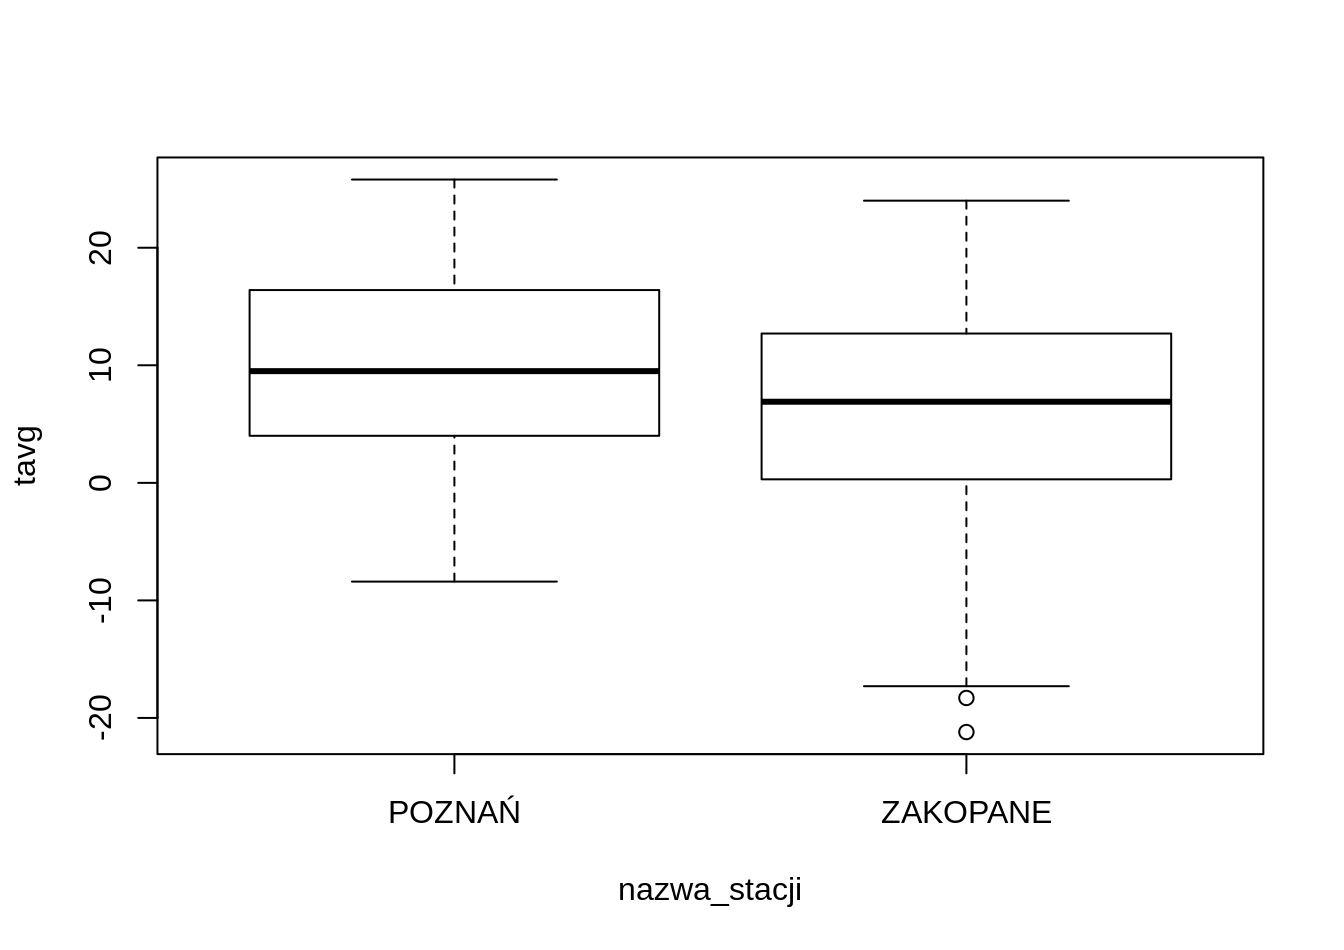
\includegraphics[width=\textwidth]{31-podsumowanie_files/figure-latex/plotex-1} 

}

\caption{Przykład wykresu utworzonego przy pomocy funkcji boxplot().}\label{fig:plotex}
\end{figure}

Powyższy wykres może być zmodyfikowany używając dodatkowych argumentów (np. \texttt{main} dodający tytuł czy \texttt{col} zmieniający kolor pudełek) czy też dodatkowych funkcji pozwalających na dodanie legendy (funkcja \texttt{legend}) czy też tekstu (funkcja \texttt{text}).
Inne dostępne wbudowane funkcje do tworzenia wykresów to, między innymi, \texttt{hist()} czy \texttt{barplot()} budujące histogramy oraz wykresy słupkowe.

Najbardziej elastyczną funkcją do tworzenia wykresów w R jest \texttt{plot()}.
Domyślnie, gdy użytkownik poda wartości numeryczne dla argumentów \texttt{x} i \texttt{y} pozwala ona tworzyć wykresy punktowe.
Jej zachowanie i wynik będzie jednak inne w zależności od tego jakiej klasy będzie obiekt wejściowy, przykładowo inaczej wyświetlony zostanie model liniowy, efekt grupowania hierarchicznego, czy też wynik testu statystycznego.

Oprócz wbudowanych w R funkcji graficznych, istnieje też szereg dodatkowych pakietów służących do wizualizacji danych.
Wśród nich najpopularniejszym jest \textbf{ggplot2} \citep{R-ggplot2}.
Ten pakiet jest implementacją założeń zawartych w książce Grammar of Graphics \citep{wilkinsonGrammarGraphics2005}.
Główną funkcją tego pakietu jest \texttt{ggplot()}, która przyjmuje dane wejściowe w postaci ramki danych.
Wewnątrz tej funkcji następuje wywołanie kolejnej funkcji \texttt{aes}, gdzie definiowane są kolejne kolumny, które mają być wyświetlone na osiach wykresów oraz określają kolor, kształt, wielkość i inne elementy.
Kolejnym krokiem jest określenie typu wykresu poprzez połączenie poprzedniej funkcji (używając operatora \texttt{+}) z jedną z wielu funkcji rozpoczynających się od \texttt{geom\_}.
Przykładowo, do stworzenia wykresu pudełkowego służy \texttt{geom\_boxplot()} (rycina \ref{fig:ggplotex}).

\begin{Shaded}
\begin{Highlighting}[]
\KeywordTok{library}\NormalTok{(ggplot2)}
\KeywordTok{ggplot}\NormalTok{(met, }\KeywordTok{aes}\NormalTok{(nazwa_stacji, tavg)) }\OperatorTok{+}\StringTok{ }\KeywordTok{geom_boxplot}\NormalTok{()}
\end{Highlighting}
\end{Shaded}

\begin{figure}[H]

{\centering 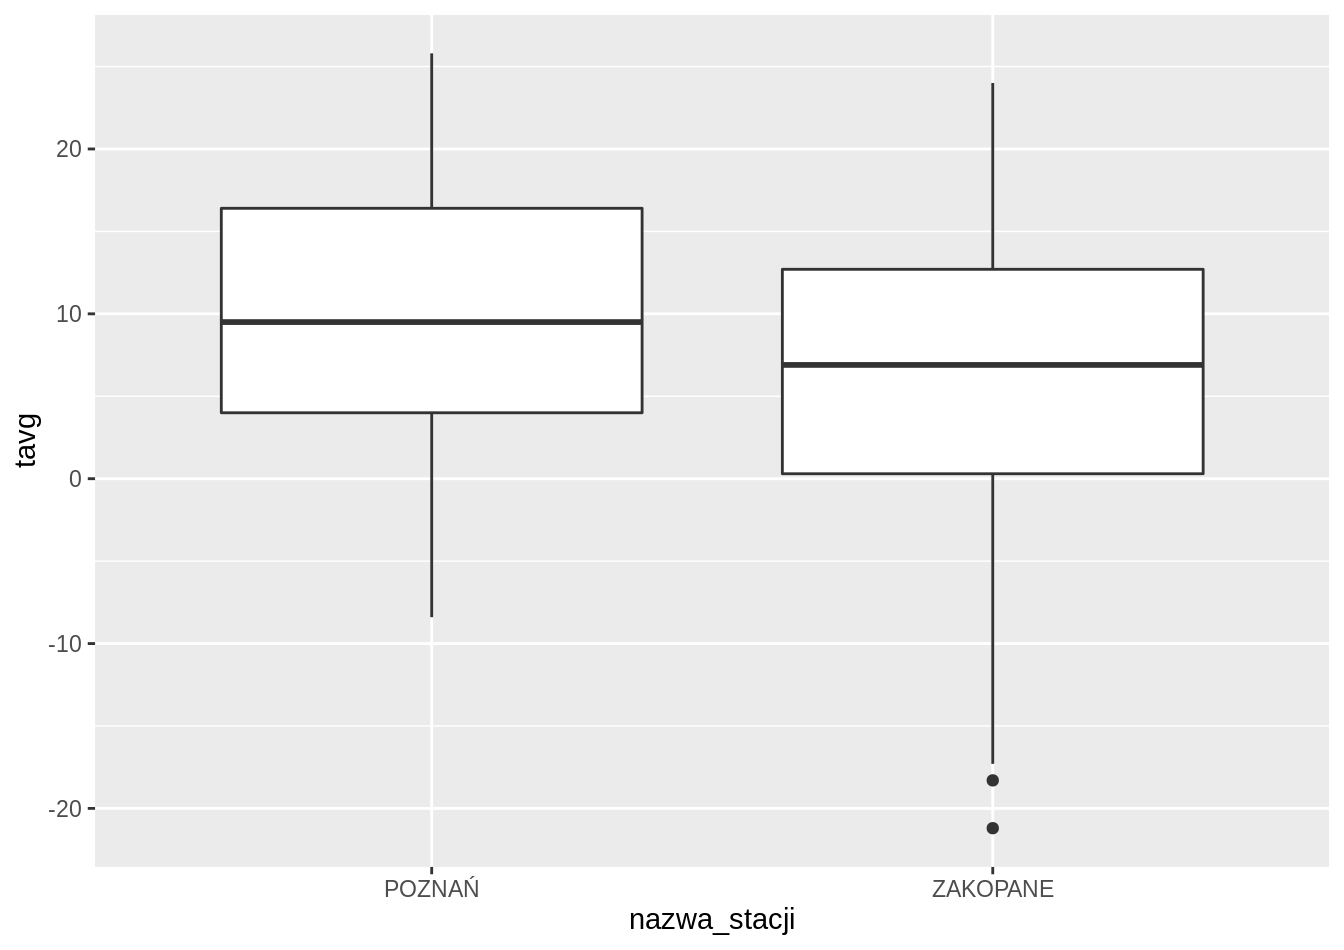
\includegraphics[width=\textwidth]{31-podsumowanie_files/figure-latex/ggplotex-1} 

}

\caption{Przykład wykresu utworzonego z użyciem pakietu ggplot2.}\label{fig:ggplotex}
\end{figure}

Pełna dokumentacja pakietu \textbf{ggplot2} znajduje się na stronie \url{http://docs.ggplot2.org}.

\hypertarget{analiza-danych}{%
\section{Analiza danych}\label{analiza-danych}}

R jest jednym z języków programowania najczęściej używanych w analizie danych\footnote{Analiza danych często jest określana również jako \href{https://en.wikipedia.org/wiki/Data_science}{data science}.}.
Jest to wynikiem szeregu przyczyn, w tym dużej liczby wbudowanych w R funkcji statystycznych oraz graficznych.
Dodatkowo, ramka danych, jeden z podstawowych obiektów w R, może być utożsamiany z arkuszem kalkulacyjnym czy tabelą z bazy danych - najpopularniejszych form przechowywania różnorakich danych.
Ta forma obiektu, złożonego z kolumn (zmienne) i wierszy (obserwacje), jest reprezentacją, która uławia czyszczenie, przetwarzanie i analizowanie danych.

Inną przyczyną popularności R do analizy danych jest grupa pakietów zbiorczo określana jako \emph{tidyverse}.
Jest to spójny zbiór pakietów pozwalających na wykonywanie kolejnych czynności analizy danych.
Na samym początku obejmuje to pakiety poświęcone wczytywaniu danych w różnych formatach, w tym poznane w rozdziale \ref{io} pakiety \textbf{readr} \citep{R-readr} oraz \textbf{readxl} \citep{R-readxl}.
Kolejnym krokiem jest porządkowanie danych, polegające, na przykład, na zmianie struktury ramki danych gdzie wartości jakiejś zmiennej stają się nazwami kolumn.
W tym etapie można użyć pakiet \textbf{tidyr} \citep{R-tidyr}.

Dane w odpowiedniej postaci można następnie przetwarzać, np. tworzyć nowe zmienne na postawie przeliczania już istniejących czy też wyliczać ich podsumowania używając pakietu \textbf{dplyr} \citep{R-dplyr}.
Tak przetworzone dane następnie są często wizualizowane używając pakietu \textbf{ggplot2} \citep{R-ggplot2} lub też w ich oparciu budowane są \href{https://github.com/tidymodels/tidymodels}{modele}.
Ma to na celu zrozumienie posiadanych danych oraz zależności czy zjawisk które opisują.

W ramach grupy pakietów \textbf{tidyverse} często stosuje się operator \texttt{\%\textgreater{}\%} (ang. \emph{pipe}) z pakietu \textbf{magrittr} \citep{R-magrittr}.
Pozwala on na łączenie kilku oddzielnych funkcji w jedno zapytanie.
Działanie tego operatora polega na tym, że wynik jednej działania jednej funkcji staje się automatycznie pierwszym argumentem w kolejnej funkcji (rycina \ref{fig:tidyverse-example}).

\begin{Shaded}
\begin{Highlighting}[]
\KeywordTok{library}\NormalTok{(magrittr)}
\NormalTok{readxl}\OperatorTok{::}\KeywordTok{read_excel}\NormalTok{(}\StringTok{"https://github.com/Nowosad/elp/raw/master/pliki/dane_meteo.xlsx"}\NormalTok{) }\OperatorTok\StringTok{ }
\StringTok{  }\NormalTok{tidyr}\OperatorTok{::}\KeywordTok{gather}\NormalTok{(}\DataTypeTok{key =} \StringTok{"zmienna"}\NormalTok{, }\DataTypeTok{value =} \StringTok{"wartosc"}\NormalTok{, tavg}\OperatorTok{:}\NormalTok{precip) }\OperatorTok
\StringTok{  }\NormalTok{dplyr}\OperatorTok{::}\KeywordTok{mutate}\NormalTok{(}\DataTypeTok{data =} \KeywordTok{as.Date}\NormalTok{(}\KeywordTok{paste}\NormalTok{(rok, miesiac, dzien, }\DataTypeTok{sep =} \StringTok{"-"}\NormalTok{))) }\OperatorTok\StringTok{ }
\StringTok{  }\NormalTok{ggplot2}\OperatorTok{::}\KeywordTok{ggplot}\NormalTok{(ggplot2}\OperatorTok{::}\KeywordTok{aes}\NormalTok{(data, wartosc)) }\OperatorTok{+}
\StringTok{  }\NormalTok{ggplot2}\OperatorTok{::}\KeywordTok{geom_line}\NormalTok{() }\OperatorTok{+}
\StringTok{  }\NormalTok{ggplot2}\OperatorTok{::}\KeywordTok{facet_grid}\NormalTok{(zmienna}\OperatorTok{~}\NormalTok{nazwa_stacji, }\DataTypeTok{scale =} \StringTok{"free_y"}\NormalTok{)}
\end{Highlighting}
\end{Shaded}

\begin{figure}[H]

{\centering 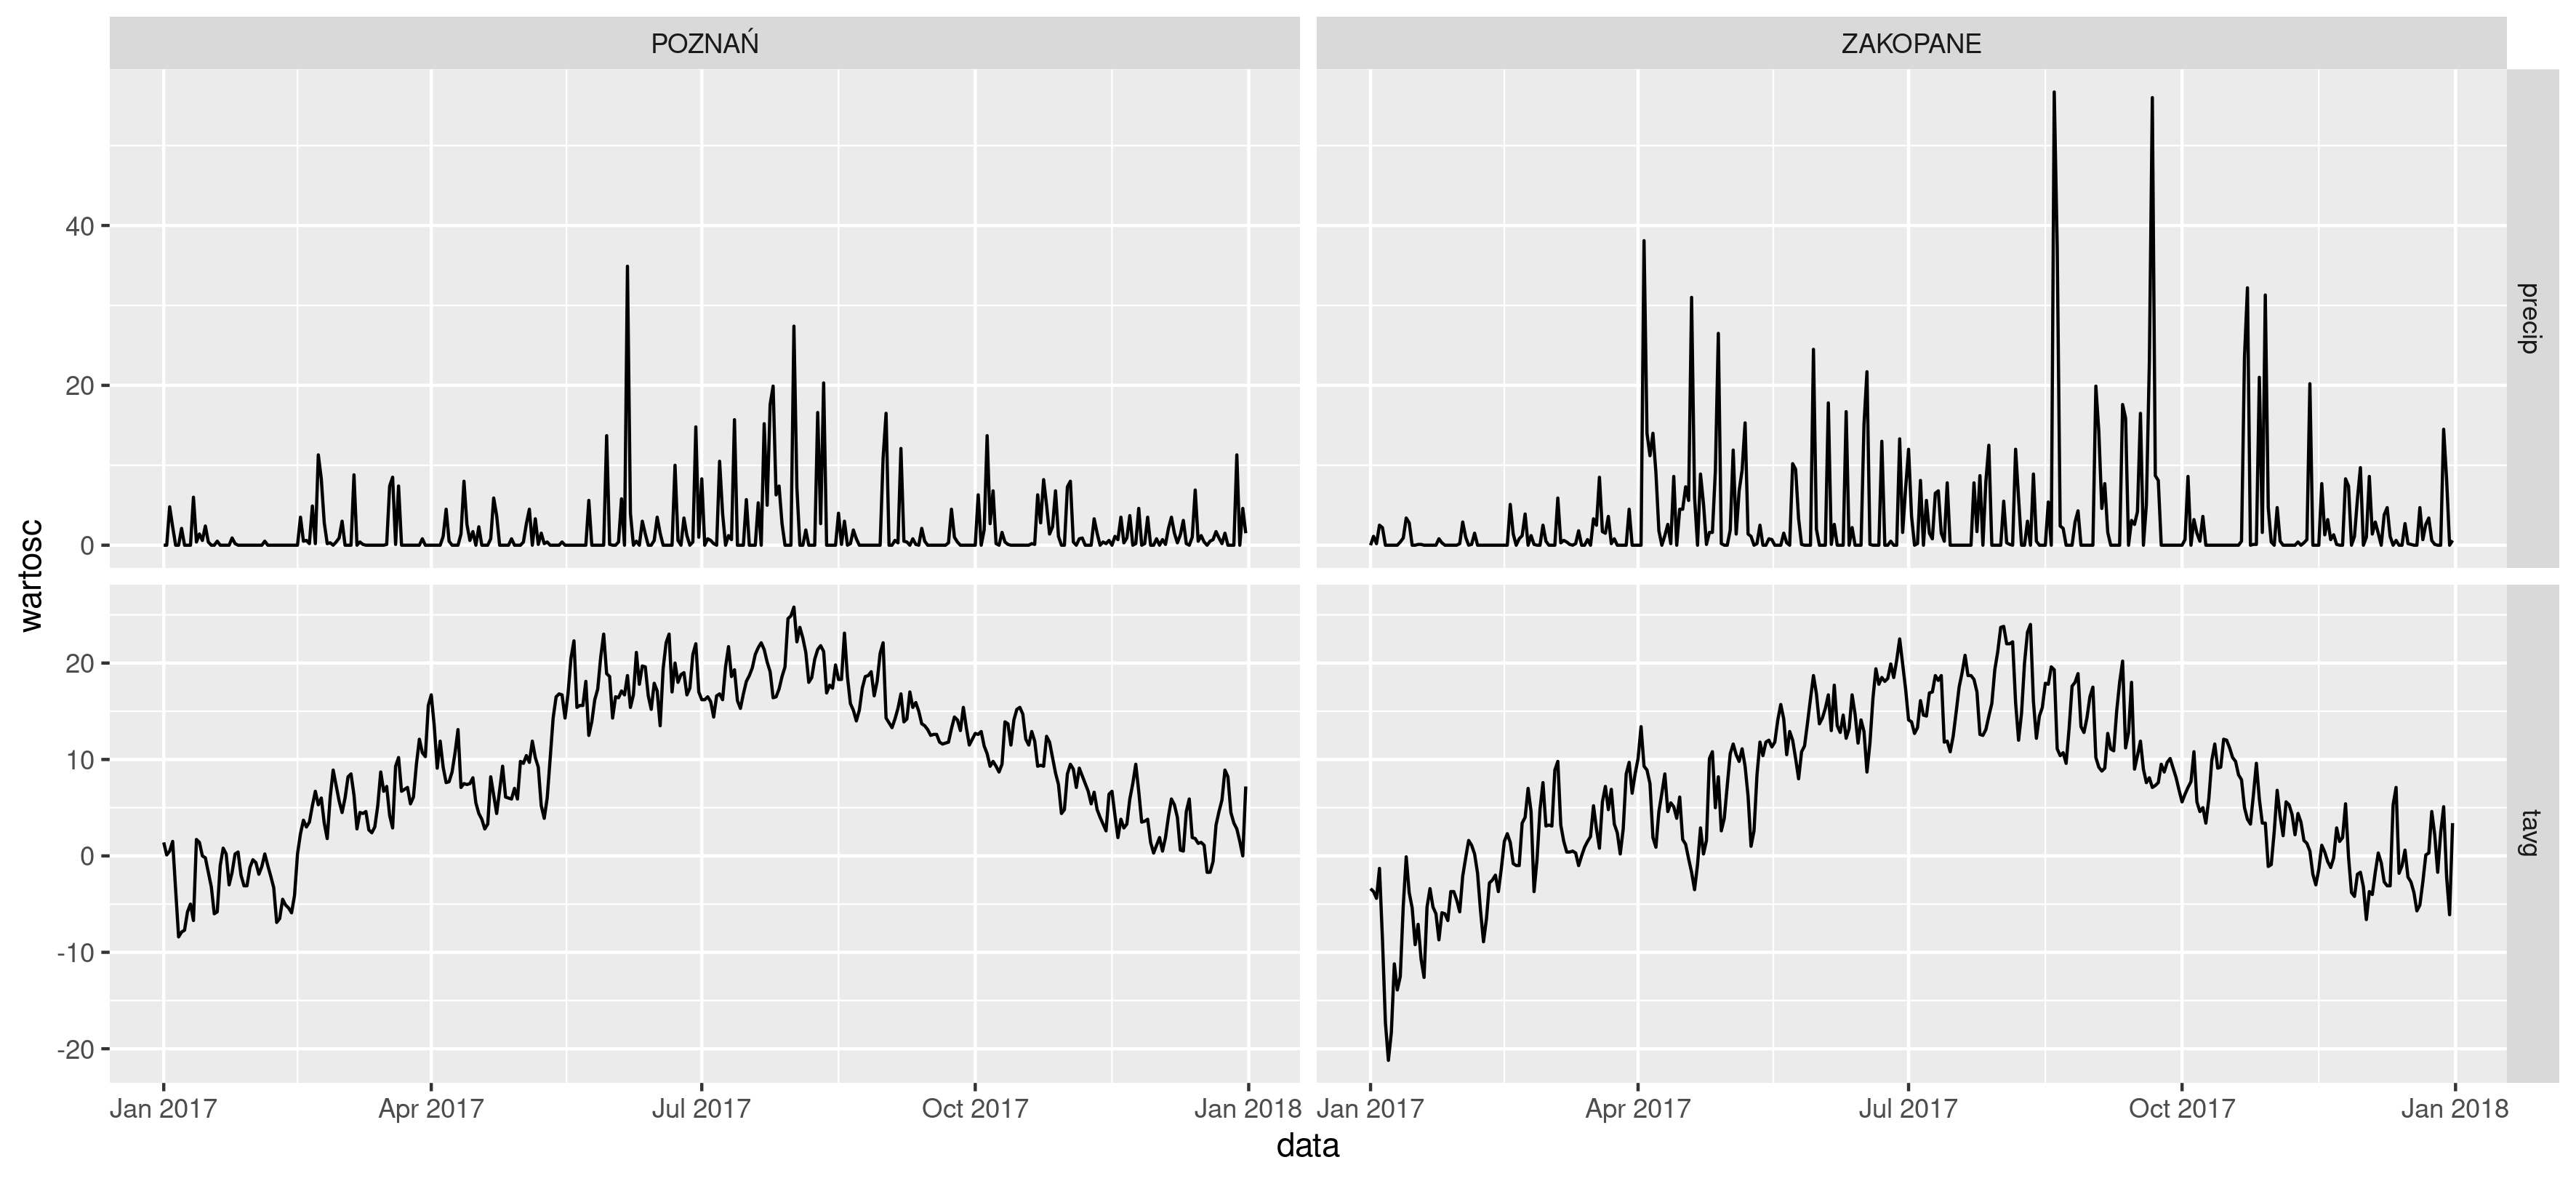
\includegraphics[width=\textwidth]{images/tidyverse-example} 

}

\caption{Przykład wyniku użycia pakietów z grupy tidyverse.}\label{fig:tidyverse-example}
\end{figure}

Pełne wprowadzenie do koncepcji \emph{tidyverse} można znaleźć w książce \href{https://r4ds.had.co.nz/}{R for Data Science} \citep{wickham2016r}.

Zrozumienie zależności czy zjawisk jest bardzo rzadko ostatnim etapem - równie istotne jest przekazanie tych wyników wybranej grupie odbiorców w odpowiedni sposób.
Do tego celu może posłużyć R Markdown (jego podstawy zostały opisane w sekcji \ref{dokumentacja-pakietu})
R Markdown pozwala na tworzenie dokumentów w różnych formatach (html, pdf, docx, itd.), prezentacji, stron internetowych, książek\footnote{Ta książka również powstała używająć R Markdown.} i wiele innych.
Po szczegółowe instrukcje jak używać tego języka warto zajrzeć do książki
\href{https://bookdown.org/yihui/rmarkdown/}{R Markdown: The Definitive Guide} \citep{xieMarkdownDefinitiveGuide2018}.

\hypertarget{inne-zastosowania}{%
\section{Inne zastosowania}\label{inne-zastosowania}}

Wcześniejsze dwie sekcje pokazywały bardzo szerokie zastosowania R - analizować czy wizualizować można zarówno dane o temperaturze powietrza jak i wyniki wyborów prezydenckich.
W związku z czym, w R istnieje także znacząca liczba pakietów stworzonych do bardziej specjalistycznych i szczegółowych celów.
Można to zobaczyć przeglądając tzw. \emph{task views} - listy pakietów zagregowane według podobnej tematyki znajdujące się pod adresem \url{https://cran.r-project.org/web/views/}.
Obejmuje to bardzo szeroki przekrój tematów - od list poświęconych projektowaniu prób klinicznych, poprzez przetwarzanie języka naturalnego, skończywszy na ekonometrii i analizach finansowych\footnote{Dodatkowo istnieje specjalne repozytorium Bioconductor poświęcone pakietom R dotyczącym zagadnień bioinformatycznych.}.

Wśród tych list znajduje się także jedna poświęcona analizie danych przestrzennych.
Opisuje ona, między innymi, takie pakiety jak \textbf{sf}, pozwalający na wczytywanie, przetwarzanie i zapisywanie danych wektorowych czy \textbf{tmap} ułatwiający tworzenie map.
Na poniższym przykładzie następuje dołączenie tych pakietów oraz wczytanie zbioru danych \texttt{World} zawierającego poligony krajów na świecie i podstawowe informacje o nich.
Dalej następuje dodanie tych danych do wyświetlenia i wybór odwzorowania przestrzennego używając funkcji \texttt{tm\_shape()}, po czym te dane są wyświetlone w postaci poligonów (funkcja \texttt{tm\_polygons()}), gdzie kolory poligonów wynikają z ich wartości w kolumnie \texttt{life\_exp} a tytuł legendy jest wybrany przez nas (rycina \ref{fig:tmap-example}).

\begin{Shaded}
\begin{Highlighting}[]
\KeywordTok{library}\NormalTok{(sf)}
\KeywordTok{library}\NormalTok{(tmap)}
\KeywordTok{data}\NormalTok{(World)}
\KeywordTok{tm_shape}\NormalTok{(World, }\DataTypeTok{projection =} \StringTok{"robin"}\NormalTok{) }\OperatorTok{+}\StringTok{ }
\StringTok{    }\KeywordTok{tm_polygons}\NormalTok{(}\DataTypeTok{col =} \StringTok{"life_exp"}\NormalTok{, }
                \DataTypeTok{title =} \StringTok{"Oczekiwana dalsza }\CharTok{\textbackslash{}n}\StringTok{długość życia"}\NormalTok{)}
\end{Highlighting}
\end{Shaded}

\begin{figure}[H]

{\centering 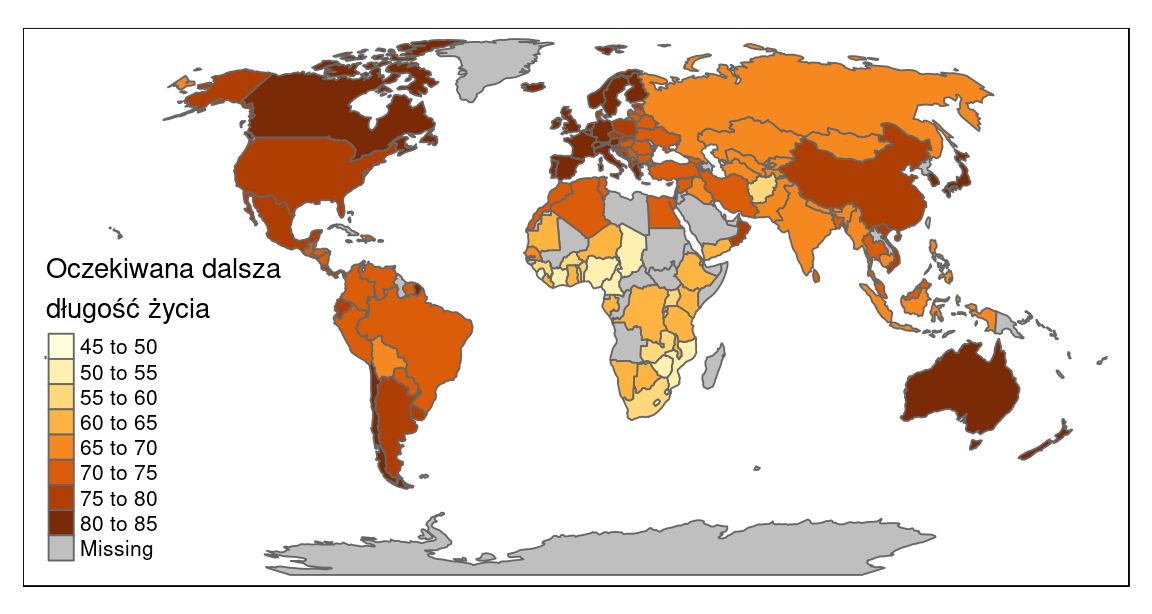
\includegraphics[width=\textwidth]{images/tmap-example} 

}

\caption{Przykład działania pakietu tmap.}\label{fig:tmap-example}
\end{figure}

Podstawy działania na danych przestrzennych zawiera książka \href{https://geocompr.robinlovelace.net/}{Geocomputation with R} \citep{lovelace2019geocomputation}.

\hypertarget{programowanie-w-r}{%
\section{Programowanie w R}\label{programowanie-w-r}}

Wcześniejsze sekcje opisywały różne obszary zastosowań R, ale nie pokazywały w jaki sposób rozwijać umiejętności programowania w tym języku.
Najprostszym sposobem jest używanie R jak najczęściej.
Nauka języka programowania przebiega wówczas naturalnie - wraz ze znaleziskiem rozwiązania kolejnego problemu czy rozwiązaniem kolejnego zadania.

Często jednak, nie jesteśmy w stanie stwierdzić czy ten sposób rozwiązania jest optymalny, lub też napotykamy sytuacje w których nie wiemy jak się do nich odnieść.
Wówczas szczególnie istotna jest inna umiejętność - czytania kodu innych osób\footnote{Read the Source, Luke.}.
Większość pakietów R jest otwartoźródłowych - ich kod jest dostępny online i każda chętna osoba ma do niego dostęp\footnote{Dostępny jest także kod źródłowy samego języka R.
  Można go znaleźć pod adresem \url{https://github.com/wch/r-source}.}.
Kod pakietów R można, między innymi, znaleźć w serwisie GitHub.
Wszystkie pakiety znajdujące się w repozytorium CRAN można znaleźć pod adresem \url{https://github.com/cran}.
Inną możliwością jest samodzielne wyszukanie kodu pakietu używając wyszukiwarki GitHub - \url{https://github.com/search}.

Przykładowo, pod adresem \url{https://github.com/karthik/wesanderson} znajduje się kod źródłowy pakietu \textbf{wesanderson} \citep{R-wesanderson}.
Ten pakiet zawiera funkcje tworzące palety kolorystyczne inspirowane filmami reżysera \href{https://en.wikipedia.org/wiki/Wes_Anderson}{Wesa Andersona}.
Kod R będący podstawą działania tego pakietu znajduje się w folderze \texttt{R/}\footnote{Szczególnie \texttt{R/colors.R}.}.
Dodatkowo, niektóre pakietu zawierają kod z innych języków programowania (np. C lub C++), który wymaga wcześniejszej kompilacji.
Taki kod znajduje się w folderze \texttt{src/}.

\hypertarget{co-dalej}{%
\section{Co dalej?}\label{co-dalej}}

Programowanie to nie tylko pisanie kodu.
Obejmuje to też wiele innych czynności, takich jak stosowanie optymalnych algorytmów czy narzędzi programistycznych.
Istnieje wiele książek poświęconych kwestii algorytmów, wśród których najbardziej popularne to Introduction to Algorithms \citep{cormen2009introduction}, The Algorithm Design Manual \citep{skienaAlgorithmDesignManual2008} czy Algorithms \citep{032157351X}.
Podstawowym narzędziem programistycznym jest program do pisania kodu.
Może to być zarówno prosty edytor tekstu, taki jak \href{https://notepad-plus-plus.org/}{Notepad++}, \href{https://www.sublimetext.com/}{Sublime Text}, lub \href{https://atom.io/}{Atom} czy też~bardziej złożone zintegrowane środowisko programistyczne (IDE).
O ile narzędzia z tej pierwszej grupy są uniwersalne to w przypadku wyboru IDE warto zdecydować się~na zintegrowane środowisko programistyczne odpowiednie dla używanego języka programowania\footnote{\url{https://en.wikipedia.org/wiki/Comparison_of_integrated_development_environments}}.

Programowanie często obejmuje pracę w zespole.
Wówczas jednym ze sposobów dbania o jakość tworzonego produktu może być inspekcja kodu (ang. \emph{code review}).
Polega ona na tym, że zmiany naniesione w kodzie są~przekazywane innej osobie, która sprawdza go pod kątem błędów, spójności, stylu, zgodności z istniejącymi rozwiązaniami, itd.
Po inspekcji twórca kodu może dostać informację zwrotną, co jest dobre, a co wymaga poprawy.
W efekcie, z jednej strony wyjściowy produkt jest lepszej jakości, a z drugiej strony programista uczy się~i polepsza swoje umiejętności.

Niezależnie od używanego języka istnieje również szereg narzędzi, których znajomość~ułatwia lub czasem nawet umożliwia pracę.
Wśród nich można wyróżnić znajomość linii komend i jej możliwości \citep{krossUnixWorkbench2017} oraz języka SQL służącego do tworzenia, edycji i zarządzania relacyjnymi bazami danych \citep{beighley2007head, forta2013sams}.

Innym kierunkiem działań może być nauka kolejnego języka programowania - najlepiej takiego, którego główne zastosowanie różni się od R.
Może to być przykładowo język kompilowany, taki jak C, C++ lub Rust, którego efektem będzie bardziej wydajny program.
Co ważne, kod napisany w tych językach można łączyć z kodem R.
R posiada wbudowany interfejs do używania kodu napisanego w C (rozdział 5 z dokumentacji \href{https://cran.r-project.org/doc/manuals/R-exts.html\#System-and-foreign-language-interfaces}{Writing R Extensions} \citep{team1999writing}), łączenie kodu napisanego w C++ ułatwia znacząco pakiet \textbf{Rcpp} (\citet{R-Rcpp}; więcej informacji w rozdziale \href{https://adv-r.hadley.nz/rcpp.html}{``Rewriting R code in C++''} książki Advanced R \citep{wickham2014advanced}), a wskazówki dotyczące łączenia kodu Rust można znaleźć w repozytorium \url{https://github.com/r-rust/hellorust}.
W efekcie użytkownik może korzystać z interaktywności R, wykonując dowolne linie kodu, ale część z nich może używać wydajniejszych funkcji napisanych w językach kompilowanych.
Alternatywną drogą może być~nauka języków używanych do tworzenia i rozwijania aplikacji internetowych, w tym JavaScript czy PHP.

Pomimo już znaczącej historii, języki programowania nadal mają wiele nowego do zaoferowania.
Nieustannie następuje ich ewolucja - dodawane są~nowe możliwości, zmieniane są~istniejące funkcje, czy też~następuje poprawa wydajności.
Tworzone są również pakiety, moduły, czy biblioteki implementujące nowe pomysły, czy też ulepszające i rozszerzające dostępne oprogramowanie.
W efekcie typowy kod napisany w danym języku kilka lat temu może się różnić od tego napisanego dziś.
Powstaje też ciągle wiele nowych języków, z których tylko niewielka część~zdobywa szersze grono użytkowników.
Te języki często wprowadzają nowe podejścia i koncepcje, które później mają bezpośredni wpływ na zmiany w istniejących językach.
Języki programowania są~też~stosowane coraz częściej w wielu codzienne używanych sprzętach, w tym samochodach czy lodówkach (ang. \emph{internet of things}, IOT).

Powodzenia w dalszej przygodzie z programowaniem!

\bibliography{references.bib,packages.bib}

\end{document}
